%
\documentclass[11pt]{thesis} % draft

\title{Algorithmic Meta-Creativity}
\author{Fania Raczinski}
\date{March 2015}

% Test

\begin{document}

% \pagestyle{empty}
% \todototoc
% \setcounter{tocdepth}{1}  % needed to display the todos
% \listoftodos[List of Todos]
% \clearpage
\pagestyle{empty}

% !TEX root = ../main.tex

% \begin{titlepage}
\begin{titlingpage}
\begin{center}

Institute of Creative Technologies\\
De Montfort University

\vspace{1cm}

\textsc{\huge \href{http://fania.uk}{Fania Raczinski}}

\vspace{1.5cm}

% \includegraphics{dmu}\\[2cm]

% \textsc{\Huge \bfseries Algorithmic Meta-Creativity}
\textsc{\bfseries\scshape\sffamily \fontsize{40}{30}\selectfont Algorithmic Meta-Creativity}

\vspace{1cm}

{\huge \bfseries Creative Computing and Pataphysics for Computational Creativity}
% A pataphysical methodology for applying creativity to exploratory search

\vspace{1cm}
{\Huge \textbf{\url{pata.physics.wtf}}}
\vspace{1.5cm}

\emph{Supervisors:}\\
{Prof.\ Hongji \textsc{Yang}}\\
{Prof.\ Andrew \textsc{Hugill}}\\
{Dr.\ Sophy \textsc{Smith}}\\
{Prof.\ Jim \textsc{Hendler}}

\vspace{1.5cm}

\large \emph{A thesis submitted in partial fulfilment of the requirements\\ for the degree of Doctor of Philosophy}

\vfill

Created: {25th March 2015} --- Last Saved: {\today}\\
Wordcount: \wordcount

\end{center}
\end{titlingpage}
% \end{titlepage}


\pagestyle{fania}

% FRONT
\frontmatter
\pagestyle{fania}

\phantomsection
\addcontentsline{toc}{part}{\texorpdfstring{PREFACE}{Preface}}
\partimage[width=\textwidth]{spiral_pre.pdf}
\part{\texorpdfstring{PRE\scalebox{2.5}{\smiley{}}}{Preface}}
% !TEX root = ../main.tex

\pagestyle{empty}

\chapter{TL;DR}
\label{abstract}

{\Large \textbf{Algorithmic Meta-Creativity}} --- Fania Raczinski

\vspace{0.5cm}
ABSTRACT\footnote{``Too long; didn't read''} --- 300 words

\lipsum[1-2]

\clearpage

% !TEX root = ../main.tex

\pagestyle{empty}

\chapter{Dedication}

% \begin{IPA}
%   aɪ lʌv juː deɪv. wɪˈðaʊt juː aɪ wʊd nɒt hæv ˈfɪnɪʃt ðɪs ˈθiːsɪs. θæŋk juː fɔːr ˈɛvrɪθɪŋ.
% \end{IPA}

% \begin{IPA}
%   aɪ l2v juː deɪv. wɪˈðaʊt juː aɪ wʊd nɒt hæv ˈfɪnɪʃt ðɪs ˈθiːsɪs. θæŋk juː fɔːr ˈɛvrɪθɪŋ.
% \end{IPA}

% http://uakari.ling.washington.edu/e-linguistics/eltk.html

\textipa{abcdefghijklmnopqrstuvwxyz}
\textipa{ABCDEFGHIJKLMNOPQRSTUVWXYZ}


\begin{CJK}{UTF8}{min}
  物の哀れ
\end{CJK}

\clearpage

% !TEX root = ../main.tex

\pagestyle{empty}

\chapter{Publications}
\label{ch:pubs}

\textbf{Fania Raczinski}, Dave Everitt (2016) \emph{``Creative Zombie Apocalypse: A Critique of Computer Creativity Evaluation''}. Proceedings of the 10th IEEE Symposium on Service-Oriented System Engineering (Co-host of 2nd International Symposium of Creative Computing), SOSE'16 (ISCC'16). Oxford, UK. Pages 270--276.

\textbf{Fania Raczinski}, Hongji Yang and Andrew Hugill (2013) \emph{``Creative Search Using Pataphysics''}. Proceedings of the 9th ACM Conference on Creativity and Cognition, CC'13. Sydney, Australia. Pages 274--280.

Andrew Hugill, Hongji Yang, \textbf{Fania Raczinski} and James Sawle (2013) \emph{``The pataphysics of creativity: developing a tool for creative search''}. Routledge: Digital Creativity, Volume 24, Issue 3. Pages 237--251.

James Sawle, \textbf{Fania Raczinski} and Hongji Yang (2011) \emph{``A Framework for Creativity in Search Results''}. The 3rd International Conference on Creative Content Technologies, CONTENT'11. Rome, Italy. Pages 54--57.

\spirals

Funding was provided to attend ISCC 2016 in Oxford by Jon Bennett, Clinton Ingrams and a Graduate School Travel Award.

A travel fund has been awarded by the DMU Faculty of Technology for travel to Australia, Sydney for the Creativity and Cognition conference in July 2013.

De Montfort University has granted me a full 3 year bursary covering living costs and tuition fees.

\spirals

\todo{update}

IOCT Student Showcase 07 June 2016

Conference talk on ``Creative Zombie Apocalypse'' (by Fania Raczinski and Dave Everitt) at ISCC in Oxford, UK, 29 March 2016.

Phoenix CAS talk on ``Pata-computed Poetry'' in Leicester, UK, 14 Oct 2015.

De Montfort University Leicester Media School Launch Showcase, 05 November 2014.

De Montfort University Institute of Creative Technologies PhD showcase at the Phoenix Cube Gallery, Leicester, 15--18 August 2014.

Conference talk on ``'' at Creativity and Cognition in Syndey, Australia, 20 June 2013.

TDC talk on ``The Pataphysics of the Future'' (by Andrew Hugill, Hongji Yang and Fania Raczinski) in Leicester, UK, 13 Feb 2013.

\clearpage


\begin{SingleSpace}
\pagestyle{fania}
% \phantomsection
% \addcontentsline{toc}{chapter}{Short Contents}
% \setcounter{tocdepth}{0}% chapters and above
% \shorttoc{Short Contents}{0}
% \clearpage
\phantomsection
% \renewcommand*{\contentsname}{Long Contents}
% \setcounter{tocdepth}{1} % sections and above
\hypertarget{ch:contents}{}  % Make an anchor to the toc
\tableofcontents
\clearpage
\end{SingleSpace}

\phantomsection
% \addcontentsline{toc}{chapter}{Figures}
\pagestyle{fania}\listoffigures
\clearpage

\phantomsection
% \addcontentsline{toc}{chapter}{Tables}
\pagestyle{fania}\listoftables
\clearpage

% \phantomsection
% \addcontentsline{toc}{chapter}{List of Equations}
% \listofmyequations{}
% \clearpage

\phantomsection{}
% \addcontentsline{toc}{chapter}{Source Code}
\pagestyle{fania}\listoflistings{}
\clearpage

\phantomsection
\addcontentsline{toc}{chapter}{Acronyms}
% !TEX root = ../main.tex

% \ac  - acronym full first and then short
% \acf - acronym full again
% \acs - acronym short
% \acl - acronym long

\pagestyle{fania}

\chapter*{Acronyms}

\begin{acronym}[OULIPO]
  \acro{AMC}{Algorithmic Meta-Creativity}
  \acro{IR}{Information Retrieval}
  \acro{NLP}{Natural Language Processing}
  \acro{NLTK}{Natural Language Toolkit}
  \acro{IN}{Information Need}
  \acro{UI}{User Interface}
  \acro{SVM}{Support Vector Machine}
  \acro{AI}{Artificial Intelligence}
  \acro{AGI}{Artificial General Intelligence}
  \acro{ICCC}{International Conference on Computational Creativity}
  \acro{CompC}{Computational Creativity}
  \acro{CC}{Creative Computing}
  \acro{SP}{Speculative Computing}
  \acro{IJCrC}{International Journal of Creative Computing}
  \acro{DH}{Digital Humanities}
  \acro{TF}{Term Frequency}
  \acro{IDF}{Inverse Document Frequency}
  \acro{TDM}{Term-Document Matrix}
  \acro{API}{Application Program Interface}
  \acro{REST}{Representational State Transfer}
  \acro{HTTP}{Hypertext Transfer Protocol}
  \acro{RDF}{Resource Description Framework}
  \acro{IOCT}{Institute of Creative Technologies}
  \acro{LMS}{Leicester Media School}
  \acro{DMU}{De Montfort University}
  \acro{CAS}{Computer Arts Society}
  \acro{TDC}{Transdisciplinary Common Room}
  \acro{URL}{Uniform Resource Locator}
  \acro{JSON}{JavaScript Object Notation}
  \acro{TMPR}{Trajectory Model of Practice and Research}
  \acro{HTML}{Hypertext Markup Language}
  \acro{CSS}{Cascading Stylesheets}
  \acro{HCI}{Human Computer Interaction}
  \acro{MMCE}{Multi-dimensional Model of Creativity and Evaluation}
  \acro{SPECS}{Standardised Procedure for Evaluating Creative Systems}
  \acro{CSF}{Creative Search Framework}
  \acro{PEP}{Python Enhancement Proposal}
  \acro{BDFL}{Benevolent Dictator For Life}
  \acro{IOCCC}{International Obfuscated C Code Contest}
  \acro{OULIPO}{Ouvroir de Litt\'erature Potentielle}
  \acro{MLE}{Maximum Likelihood Estimation}
  \acro{POS}{Parts-of-Speech}
  \acro{VR}{Virtual Reality}
  \acro{AR}{Augmented Reality}
  \acro{ACC}{International Association for Computational Creativity}
  \acro{DNF}{Disjunctive Normal Form}
  \acro{YAML}{YAML Ain't Markup Language}
  \acro{CPU}{Central Processing Unit}
  \acro{EU}{European Union}
  \acro{HBP}{Human Brain Project}
  \acro{FLOPS}{Floating-Point Operations Per Second}
  \acro{IPA}{International Phonetic Alphabet}
  \acro{WWW}{World Wide Web}
\end{acronym}

% \printacronyms[style=mylong]
% \printnoidxglossary[style=mylong,type=acronym]
% \printglossary[style=mylong,type=\acronymtype]
% \printglossaries
\clearpage


% MAIN
% \pagestyle{plain}
\mainmatter
\pagestyle{fania}

\phantomsection
% these spaces mess up my partial tocs....
% \addtocontents{toc}{\protect\vspace{20pt}}
\addcontentsline{toc}{part}{\texorpdfstring{HELLO WORLD}{Introduction}}
\partimage[width=\textwidth]{spiral_hello.pdf}
\part{\texorpdfstring{H\scalebox{2.2}{$\boldsymbol\Sigma$}LL\scalebox{2.2}{$\boldsymbol\Theta$} W\scalebox{2.2}{$\boldsymbol\Theta$}RLD}{Introduction}}
\label{p:intro}
% !TEX root = ../main.tex

\chapter{Introduction}
\label{ch:intro}

\emph{Part of this research has been described in a journal article in Digital Creativity in 2013, and I presented a paper at the Creativity and Cognition conference 2013 in Sydney.}

\grule

Imagine a web search engine that does not quite return the results you expect. For example, imagine you search for "animal" and the top three results are a list of animals in the Emperor's possession, followed by instructions about embalming animals and information on a society for animal training. Google's top search results for this query on the other hand return the webpage of an action sports lifestyle brand, the Wikipedia article and a BBC page about animal videos. While there is certainly nothing wrong with Google's results, they are simply not very inspiring. The first example of search results is adapted from Jorge Luis Borges's Chinese Encyclopaedia \citep{Borges2000} \marginpar{§¶} which lists several creative definitions of the term "animal". Whilst they might not provide the kind of information we were initially seeking (if we even had a clear idea of the kind of answers we wanted), they are still perfectly valid results for the query and might even provoke a smirk upon their encounter. These are the kind of search results we are aiming for; provocative, creative, surprising, inspiring and possibly funny yet perfectly valid.

To achieve this sort of creativity in search results we propose the use of pataphysical methods. Pataphysics is highly subjective and particular and is as such very suitable for this kind of transformation from relevant to creative. We hope that the tool will prove useful as a source for information and inspiration and at the same time challenge the way we think about information retrieval on the Web. The Web is not a place limited to one discipline and in fact it has been already suggested to create a transdisciplinary field of ‘Web Science'. Our project will therefore span across several disciplines as well.

\begin{quote}
  "Given the breadth of the Web and its inherently multi-user (social) nature, its science is necessarily interdisciplinary, involving at least mathematics, [computer science], artificial intelligence, sociology, psychology, biology, and economics." \citep{Hendler2008}
\end{quote}

Over the rest of the article, we will examine how pataphysics and creativity map onto one another, give an outline of the field of information retrieval, and discuss how this new type of search could be implemented in future systems. We conclude with a short discussion and summary of the article.

\section{Problem / Motivation / Context}

Jorge Luis Borges has provided us with a very useful example to illustrate our idea. His ‘Chinese Encyclopaedia' \citep{Borges2000} lists the following results under the category of ‘animal'.

\begin{enumerate}
  \item those that belong to the Emperor,
  \item embalmed ones,
  \item those that are trained,
  \item suckling pigs,
  \item mermaids,
  \item fabulous ones,
  \item stray dogs,
  \item those included in the present classification,
  \item those that tremble as if they were mad,
  \item innumerable ones,
  \item those drawn with a very fine camelhair brush,
  \item others,
  \item those that have just broken a flower vase,
  \item those that from a long way off look like flies.
\end{enumerate}

Although these are all perfectly valid results, it is clear that they form a more creative, even poetic, view of what an animal might be than the Oxford English Dictionary's prosaic: "a living organism which feeds on organic matter".

\subsection{Syzygy Surfer}

Pataphysics can provide some useful techniques that are very suitable for creative computing. Hendler and Hugill first suggested the use of three of its principles: clinamen, syzygy and anomaly, in their "Syzygy Surfer".

\begin{quote}
  "The ambiguity of experience is the hallmark of creativity, that is captured in the essence of pataphysics. Traversing the representations of this ambiguity using algorithms inspired by the syzygy, clinamen and anomaly of pataphysics, using a panalogical mechanism applied to metadata, should be able to humanize and even poeticize the experience of searching the Web." \citep{Hendler2013}
\end{quote}

In this article we propose a new type of Web search engine, reminiscent of the experience of ‘surfing the Web'. This is in contrast to current search engines which value relevant results over creative ones. ‘Surfing' used to be a creative interaction between a user and the web of information on the Internet, but the regular use of modern search engines has changed our expectations of this sort of knowledge acquisition. It has drifted away from a learning process by exploring the Web to a straightforward process of information retrieval similar to looking up a word in a dictionary.

Hendler and Hugill introduce a new concept for a web search engine in their paper "The Syzygy Surfer: Creative Technology for the World Wide Web" \citep{Hendler2011}. This PhD research is built on their initial investigation but it should be noted that the Syzygy Surfer is purely conceptual; there is no working prototype available. In the paper, Hendler and Hugill claim that "surfing has become a term for the secure journey to a well-regarded site full of safe content" and suggest a tool that supports "surfing" the web (browse and explore) instead of searching it. Their inspirations come from Borges' "Chinese Encyclopaedia" \citep{Borges2000} (for the underlying poetic sense of unity), Jarry's Pataphysics (for the concept of patadata – data beyond metadata) and  panalogies (parallel analogies – to introduce ambiguity, since it allows various descriptions of the same object) as formulated by Singh \citep{Singh2005}. The search can be executed using three different techniques, using either a syzygy, clinamen or anomaly approach. They also mention the importance of the interface design; features of which should be as follows.

\begin{itemize}
  \item Users should be able to choose the technique for the search (syzygy, clinamen or anomaly)
  \item The system should suggest additional search terms to add to or change the query
  \item The site should have a breadcrumb trail of navigations
  \item The design should be attractive, accessible and adaptable
\end{itemize}

\subsection{Research Questions}

\begin{itemize}
  \item How can we make a search tool that is inspirational rather than informational?
  \item How can we get search results that are unexpected and yet make sense?
  \item How can we rank search results but still be true to Pataphysics philosophy?
  \item How can we represent and structure data to reflect its context, meaning and subjectivity?
  \item How can we present search results in a creative and pataphysical way?
  \item How does Pataphysics relate to creative computing?
  \item How can we use Pataphysics as inspiration for search ranking?
  \item How can we write a specifically creative algorithm?
  \item How can Semantic Web technologies help with the representation of patadata?
  \item What does it mean for search results to be creative/relevant?
\end{itemize}

\section{Aims and Objectives / Methodology}

\begin{quote}
  "Purposive without purpose" Kant
\end{quote}

The aim of this project, in simple words, is to design a tool for creative searching on the Web. It tries to create a fresh way of searching and navigating through information and content on the Internet, to bring back some of the inspirational chance encounters that were so characteristic for libraries. It tries to provide an alternative for or addition to the standard search tools, a different approach that some people might benefit from and others probably won't.

The focus of this project will be on the creation of a unique and innovative ranking algorithm(s) rather than the general architecture of the search engine. These algorithms are in essence what make this tool creative and what drive the general user experience. They will be based on a "patadata" framework and an ontology specific to the knowledge domain of the pseudo-philosophy Pataphysics.

The tool will challenge the way we understand data and metadata and suggest new meanings between them in accordance with the underlying philosophy. The way we think about information is redefined. It will create new standards or rather get rid of all previous standards and classifications. It will create new links and connections between pieces of information that are not simply based on keyword similarities but rather a more poetic sense of unity. It will be a refreshing new view compared to the structured and standardised thinking of computer scientists. It will challenge the binary logic that dominates the world of programmers and concentrate on what they would view as an illogical and unstructured system going against all standards.

The goal is also to investigate creative ways of visually presenting the tool's search results while maintaining the pataphysical philosophy. The project aims to change the way users navigate through their searches as a whole. It aims to turn a simple search into a "journey" that can be traced back to individual steps using breadcrumb trails of navigations. This breadcrumb trail could displays the list of previously visited search results and with such, provide the user with the current location and immediate search history. Being able to go back and forth or adding new constraints to a search at any given point could prove useful and fruitful for the user. It should be transparent how the tool works, how it finds the results, but not overwhelm the user with too much technical information. The user should have a choice of whether or not they want to see it.

This project combines research in science and art. It is an interdisciplinary research project.

This project has roots in disciplines such as Computer Science and Humanities.
\begin{description}
  \item [Information Retrieval]: Software Engineering, Semantic Web
  \item [Pataphysics]: Literature, Philosophy, Ontology
  \item [Creativity]: Cognitive Science, Artificial Intelligence
\end{description}

In regards to my project:
\begin{itemize}
  \item A concept implementation method is used with a descriptive-other approach
  \item A qualitative investigation into if and why the proposed search results are useful will be done
  \item Following experimental methodologies, to evaluate the proposed new solution to the problem of creative search
\end{itemize}

\begin{description}
  \item [Epistemology]: Subjective/Argumentative
  \item [Methodology]: Experimental, Interpretative, Qualitative
  \item [Methods]: Concept implementation, (Heuristic) Evaluation
\end{description}

The main aim of this project is to design a creative search tool based on an innovative ranking system inspired by the idea of Pataphysics. The investigation will specifically focus on the development of a set of search algorithms. Part of this is to develop a new semantic system to describe, compare and order information in the form of "patadata". Next to this, the aim is to investigate creative ways of visually presenting search results while maintaining the underlying pataphysical philosophy. The result will provide users with a unique search" journey" that can be traced back to individual steps using breadcrumb trails of navigations.

\section{Deliverables / Outcomes}

\begin{itemize}
  \item Design a tool for creative searching on the Web
  \item Design pataphysics inspired algorithms to model creativity in this tool
  \item Produce a proof-of-concept prototype
  \item Propose a framework for evaluating and interpreting creative search results
\end{itemize}

The outcome of this project will be a fully functioning search tool for the web. Based on a unique and innovative "ranking" algorithm, the search tool will include a patadata framework and an ontology specific to the knowledge domain of Pataphysics. It will challenge the way we understand data and metadata and suggest new relationships and meanings between them in accordance with the philosophy of Pataphysics.  Research dissemination is a crucial part in any innovative project like this, so an effort will be placed on presenting findings at conferences and publishing papers.


\subsection{Contribution to Knowledge}

Compared to the mainstream search engines available publically, my project's approach to searching will be very different. Google, for example, ranks web pages based on the number and quality of incoming hyperlinks \citep{Google2012}, while I will be using the concept of patadata (data-metadata-patadata) and semantic web technologies.

There have been interdisciplinary projects like Johanna Drucker's Speclab \citep{Drucker2009} which have similar inspirations, and literature on Pataphysics is found in several places \citep{Bok2002, Hugill2012a} although the idea of using it as an inspiration for a search engine appears to be very new \citep{Hendler2013}.

A lot of literature exists on how to model creativity on a computer [5] [7], explaining several theories on how the mind works and how to simulate this on a machine. However none of these have any kind of pataphysical inspiration and aren't applicable to search engines, so we have presented a paper on creativity in search results just recently \citep{Raczinski2013}.

\subsection{Publications}

James Sawle, \textbf{Fania Raczinski} and Hongji Yang (2011) \emph{"A Framework for Creativity in Search Results"}. The 3rd International Conference on Creative Content Technologies, CONTENT'11. Rome, Italy. Pages 54-57.

\noindent Andrew Hugill, Hongji Yang, \textbf{Fania Raczinski} and James Sawle (2013) \emph{"The pataphysics of creativity: developing a tool for creative search"}. Routledge: Digital Creativity, Volume 24, Issue 3. Pages 237-251.

\noindent \textbf{Fania Raczinski}, Hongji Yang and Andrew Hugill (2013) \emph{"Creative Search Using Pataphysics"}. Proceedings of the 9th ACM Conference on Creativity and Cognition, CC'13. Sydney, Australia. Pages 274-280.

% !TEX root = ../main.tex

\chapter{Inspirations}
\label{ch:inspirations}

\startcontents[chapters]

\vfill

\begin{alltt}\sffamily
Thought she would die of mortification,
pues jamas tuve la idea de falsificar billetes de banco,
engenders God by interior intuition,
affinant la curiosite en intuition qu'existe de.

The pale motor vessel withdrew its blue breath toward the island's horizon,
the work is a hasty and unrevised production of its author,
il eut l'intuition d'une sorte d'impuissance divine,
how Gargantua was carried eleven months in his mother's belly.

And thought himself in honor bound,
pale rayon ... -- La source pleure au loin dans,
the greatest source of the Icelanders' wealth.

I will pull down my barns,
nor breath nor motion,
but the old man was at his last gasp.
\end{alltt}

\newpage
\minicontents
\spirals

This research was heavily influenced by a few major inspirations and this chapter introduces them all.


\section{The Syzygy Surfer}
\label{s:surfer}

This PhD project is directly based on the \textit{Syzygy Surfer} \autocite{Hendler2011, Hendler2013}. Hendler and Hugill suggest the use of three pataphysical principles, namely clinamen, syzygy and anomaly, to create a new type of Web search engine reminiscent of the experience of surfing the Web using Semantic Web technologies. This is in contrast to current Web search engines which value relevant results over creative ones.

`Surfing' used to be a creative interaction between a user and the web of information on the Internet, but the regular use of modern search engines has changed our expectations of this sort of knowledge acquisition. It has drifted away from a learning process by exploring the Web to a straightforward process of information retrieval similar to looking up a word in a dictionary.

\begin{quotation}
  The ambiguity of experience is the hallmark of creativity, that is captured in the essence of pataphysics. Traversing the representations of this ambiguity using algorithms inspired by the syzygy, clinamen and anomaly of pataphysics, using a panalogical mechanism applied to metadata, should be able to humanize and even poeticize the experience of searching the Web. \sourceatright{\autocite{Hendler2013}}
\end{quotation}

Their inspirations come from Borges \citeyear{Borges2000} (for the underlying poetic sense of unity), Jarry's pataphysical principles \citeyear{Jarry1996} and Singh's panalogies (parallel analogies – to introduce ambiguity, since it allows various descriptions of the same object) \citeyear{Singh2005}.

\todo{mention MInsky}

My project has since moved on from the idea of using the Semantic Web to create the search tool and uses the concept of antinomy rather than anomaly as one of its three algorithms. One of my original ideas based on the Syzygy Surfer was to create an standard ontology of creativity using Semantic Web technologies. I quickly ran into the following problem though: the idea of standards is totally opposed to that of surprise - which plays a role in creativity. Pataphysics in particular is fond of breaking standards (e.g.\ exceptions, contradictions, etc.). But standards are a key building block of the Semantic Web. A common ontology of creativity might be useful in some cases but nevertheless contradicts the use of pataphysics.


\section{Faustroll's Library of Equivalent Books}
\label{s:faustlib}

The artefact created to demonstrate the search algorithms---\url{pata.physics.wtf}---uses two collections of texts rather than the open Web as source material\marginnote{§~\ref{ch:implementation}}. One of these corpora is based on the fictional library of `equivalent books' from Alfred Jarry's \textit{Exploits and Opinions of Dr.\ Faustroll, $'$Pataphysician} \citeyear[p.10-12]{Jarry1996}

The library also contains three prints (a poster of `Jane Avril' by Toulouse-Lautrec, an advert for the `Revue Blanche' by Bonnard, and a portrait of Doctor Faustroll by Aubrey Beardsley) and a picture `Saint Cado' by the Oberthuer printing house of Rennes.\autocite[p.12]{Jarry1996}.\marginnote{\faicon{picture-o}~\ref{fig:libimgs}}

This library contains the following books.

\begin{quotation}
  \begin{enumerate}
    \item BAUDELAIRE, a volume of E.A. POE translations.
    \item BERGERAC, \textit{Works}, volume II, containing the \textit{History of the States and Empires of the Sun}, and the \textit{History of Birds}.
    \item \textit{The Gospel according to} SAINT LUKE, in Greek.
    \item BLOY, \textit{The Ungrateful Beggar}.
    \item COLERIDGE, \textit{The Rime of the ancient Mariner}.
    \item DARIEN, \textit{The Thief}.
    \item DESBORDES-VALMORE, \textit{The Oath of the Little Men}.
    \item ELSKAMP, \textit{Illuminated Designs}.
    \item An odd volume of the \textit{Plays} of FLORIAN\@.
    \item An odd volume of \textit{The Thousand and One Nights}, in the GALLAND translation.
    \item GRABBE, \textit{Scherz, Satire, Ironie und tiefere Bedeutung}, comedy in three acts.
    \item KAHN, \textit{The Tale of Gold and of Silence}.
    \item LAUTREAMONT, \textit{The Lays of Maldoror}.
    \item MAETERLINCK, \textit{Aglavaine and Selysette}.
    \item MALLARME, \textit{Verse and Prose}.
    \item MENDES, \textit{Gog}.
    \item \textit{The Odyssey}, Teubner's edition.
    \item PELADAN, \textit{Babylon}.
    \item RABELAIS\@.
    \item JEAN DE CHILRA, \textit{The Sexual Hour}.
    \item HENRI DE REGNIER, \textit{The Jasper Cane}.
    \item RIMBAUD, \textit{The Illuminations}.
    \item SCHWOB, \textit{The Childrens' Crusade}.
    \item Ubu Roi.
    \item VERLAINE, \textit{Wisdom}.
    \item VERHAEREN, \textit{The Hallucinated Landscapes}.
    \item VERNE, \textit{Voyage to the Center of the Earth}.
  \end{enumerate}
\end{quotation}

\begin{figure}[!htbp]
\centering
\begin{minipage}{.45\linewidth}
  \includegraphics[width=\linewidth]{JaneAvril}
%   \caption[Toulouse-Lautrec's `Jane Avril']{Toulouse-Lautrec's `Jane Avril'}
% \label{fig:toulouse}
\end{minipage}
\hspace{.05\linewidth}
\begin{minipage}{.45\linewidth}
  \includegraphics[width=\linewidth]{RevueBlanche}
%   \caption[Bonnard's `Revue Blanche']{Bonnard's `Revue Blanche'}
% \label{fig:bonnard}
\end{minipage}
\vspace{.05\linewidth}
\begin{minipage}{.45\linewidth}
  \includegraphics[width=\linewidth]{DocteurFaustroll}
%   \caption[Beardsley's `Docteur Faustroll']{Beardsley's `Docteur Faustroll'}
% \label{fig:beardsley}
\end{minipage}
\hspace{.05\linewidth}
\begin{minipage}{.45\linewidth}
  \includegraphics[width=\linewidth]{SaintCado}
%   \caption[Oberthuer's `Saint Cado']{Oberthuer's `Saint Cado'}
% \label{fig:oberthuer}
\end{minipage}
\caption[Jane Avril, Revue Blanche, Docteur Faustroll and Saint Cado]{Toulouse-Lautrec's \textit{Jane Avril} (top-left), Bonnard's textit{Revue Blanche} (top-right), Beardsley's \textit{Docteur Faustroll} (bottom-left) and Oberthuer's \textit{Saint Cado} (bottom-right)}
\label{fig:libimgs}
\end{figure}
\todo{add citations for these images}


\section{100.000.000.000.000 Poems}
\label{s:queneau}

The interface design\marginnote{§~\ref{s:poetry}} of some of my search results is directly inspired by
Raymond Queneau's \textit{Cent Mille Milliards de Poèmes} \citeyear{Queneau1961}, a prime example of Oulipian art. The book is essentially made up of \num{10} pages containing one sonnet each. Each page however is split into \num{14} thin strips, one for each line. This means that mathematically there are $10^{14}$ possible poems to be read by combining different lines every time. My implementation of this resulted in a sonnet, each line of which can be changed individually using mouse clicks.

\begin{figure}[!htbp]
\centering
\begin{minipage}{.45\linewidth}
  \includegraphics[width=\linewidth]{queneau1}
\end{minipage}
\hspace{.05\linewidth}
\begin{minipage}{.45\linewidth}
  \includegraphics[width=\linewidth]{queneau2}
\end{minipage}
\caption[Queneau's `Cent Mille Milliards de Poèmes']{Raymond Queneau's `Cent Mille Milliards de Poèmes'\footnotemark}
\label{fig:queneau12}
\end{figure}
\footnotetext{Images of Queneau's book in the Gallimard 2006 edition by Martin Pyper \url{http://www.mestudio.info/2010/02/28/one-hundred-thousand-billion-poems/}}
\todo{place footnote text on correct page on final runthrough}


\section{Celestial Emporium of Benevolent Knowledge}
\label{s:borges}

Jorge Luis Borges mentions a `Chinese Encyclopaedia' called the \emph{Celestial Emporium of Benevolent Knowledge} in the short story ``The Analytical Language of John Wilkins'' \citeyear{Borges2000}. It is a primary inspiration for this project, originally identified by \autocite{Hendler2011, Hendler2013}. It lists the following results under the category of `animal'.

\begin{quotation}
\begin{enumerate}
  \item those that belong to the Emperor,
  \item embalmed ones,
  \item those that are trained,
  \item suckling pigs,
  \item mermaids,
  \item fabulous ones,
  \item stray dogs,
  \item those included in the present classification,
  \item those that tremble as if they were mad,
  \item innumerable ones,
  \item those drawn with a very fine camelhair brush,
  \item others,
  \item those that have just broken a flower vase,
  \item those that from a long way off look like flies.
\end{enumerate}
\end{quotation}

Although these are obviously all perfectly valid results, it is clear that they form a more creative, even poetic, view of what an animal might be than the Oxford English Dictionary's prosaic: `a living organism which feeds on organic matter' \citeyear{OEDanimal}. This poetic form of order or structure was a direct inspiration for the results generated by this project's exploratory search tool \url{pata.physics.wtf}.


\section{Metaphorical Search Engine Yossarian}
\label{s:yossarian}

Yossarian is a creative search engine which claims to return ``diverse and unexpected results'' \citeyear{Yossarian2015}. It is probably the closest thing to `related work' that exists for this project. Being a commercial product it is hard to find reliable details on precisely how their search engine works. The site seems well marketed but its functionality is shrouded in mystery. However, they argue that

\begin{quotation}
  Yossarian makes the process of generating new ideas faster, while also improving its quality. This creative search engine helps people discover new perspectives, conceptual directions, creative insights, and allowing collaboration and feedback from a creative global community. \sourceatright{\autocite{Yossarian2015}}
\end{quotation}

They also claim to be inspired by metaphors and that generating lateral connections can diversify users ideas and help understand conceptual relationships between things through a `creative graph'.

The site started in a public alpha release in 2012. At the time it consisted of simple image search. In December 2015 a complete re-design was released \autocite{YossarianEmail} which turned the search engine into more of a mind map tool.

\begin{quotation}
  Idea Boards you can now visually jump from idea to idea and build your own custom collection of links. It's a powerful new kind of mind map powered by search, and a radical departure from traditional search engine interfaces. \sourceatright{\autocite{YossarianEmail}}
\end{quotation}

While they do boldly call themselves ``the world's first creative search engine'' \autocite{Yossarian2015} it is impossible to know how their algorithms really work and as such how similar out projects are. The recently released mind map functionality brings up those `lateral connections' in a relationship graph form, in fact there is a slider that lets users adjust how creative they want their results to be---from literal to lateral.

This search engine appeared some time after I began my PhD research and has been slow to develop. It was hard to find any concrete inspiration from it due to its secrecy and pre-release status. While the marketing and `arty bollocks'\footnote{\url{http://www.artybollocks.com/}} is great, their aim seems to be very different from mine.

\todo{remove casual critic stuff}


\section{The Library of Babel}
\label{s:babel}

The \textit{Library of Babel} is a short story by Jorge Luis Borges \citeyear{Borges1964}. It envisions a universe, called `the Library', which is composed of `an indefinite and perhaps infinite number of hexagonal galleries' containing every possible book every conceived and not yet conceived.

The specific artefact of inspiration for my project is a website implementing a miniature form of this library\footnote{\url{https://libraryofbabel.info/}} created by Jonathan Basile \citeyear{Basile2015}. Instead of containing every single book possible, it `only' contains every single page possible---which is, at \num{3200} characters per page and \num{29} possible characters, still a lot.

Basile claims to use a `pseudo-random number generating algorithm' (combining modular arithmetic and bit-shifting operations) to produce all $29^{3200}$ pages without needing to store anything on disk.

\begin{quotation}
  The pages of rational text which this algorithm can locate are rarer than a single grain of sand in that collection, yet intrinsically no more meaningful.
  [\ldots]
  One can find only text one has already written, and any attempt to find it in among other meaningful prose is certain to fail. The tantalizing promise of the universal library is the potential to discover what hasn’t been written, or what once was written and now is lost. But there is still no way for us to find what we don’t know how to look for.
  [\ldots]
  Nonetheless, the library contains its own sort of poetry and revelation, and even this disappointment can provide a moment of clarity. \sourceatright{\autocite{Basile2015}}
\end{quotation}

It is hard to say what exactly influenced my project most. I think the idea of computationally generating this massive library is fantastic---and absurd. Perhaps this is a feature we share.


\section{Oulipo}
\label{s:oulipo}

\todo{replace all references to Queneau with an abbreviation using 10to the power of xyz to shorten the title...}

The \ac{OULIPO} is an originally literary movement\footnote{It has since spread to other disciplines. The generic term for oulipian groups is OUXPO (``Ouvroir d'X Potentielle''), where the X can be replaced with whatever particular subject area you like (typically in french): fine art---OUPEINPO, music---OUMUPO, etc.} from the 1960's, originating in France as a subcommittee of the ``Coll\`{e}ge de \'Pataphysique''. It therefore has roots in pataphysics although it eventually separated and became a standalone group. Their main philosophy perhaps is to use constraints in order to enhance creative output. Some examples of techniques, taken from \autocite{Mathews2005}, invented and used by them are shown below (and many more can be seen in chapter~\ref{ch:pataphysics} in tables~\ref{tab:oulipo1} and~\ref{tab:oulipo2}\marginnote{\faicon{table}~\ref{tab:oulipo1} + \ref{tab:oulipo2}}).

\begin{description}
  \item[N+7] Invented by Jean Lescure. It's a simple method of replacing each noun with the next seventh noun in a dictionary. For example: \textit{tree} $\rightarrow$ \textit{trend}, \textit{shoreline} $\rightarrow$ \textit{shotgun}\footnote{Generated using \url{http://www.spoonbill.org/n+7/}.}.
  \item[Algol poetry] Algol (Algorithmic Oriented Language) is a programming language from 1960 which at the time consisted of only \num{24} words. It was used to write poetry given the restricted vocabulary of the language only (see example below in figure~\ref{fig:poems}).
  \item[Melting snowball] A technique by which each line in a text has one less character than the preceding one resulting in a structure as shown in figure~\ref{fig:poems}.
  \item[Paul Braffort] Paul Braffort wrote a program in 1975 to generate versions of Queneau's \num{100} thousand million poems. It used the reader's name and the time it took to write it to determine which poem to display. He did a similar thing with Italo Calvino to write a story that has a very large number of possible outcomes which can be reduced by the reader by making certain choices.
  \item[Mathew's Algorithm] In the 1970's Harry Mathews created this procedure of generating results. It is based on permutation of characters, words, symbols, numbers, etc. See figure~\ref{fig:poems}.
\end{description}

\begin{quotation}
  [The use of computers] became an instrument, not of combinatorial accumulation, but of anti-combinatorial reduction. It served not to create combinations but to eliminate them.\sourceatright{\autocite[p.131]{Mathews2005}}
\end{quotation}

\begin{figure}[!htbp]
\begin{minipage}{.42\linewidth}
  \settowidth{\versewidth}{while channel not false} 
  \indentpattern{00001}
  \begin{verse}[\versewidth]
  \begin{patverse}\ttfamily
    ~~~~~~~\textit{Table}\\
    Begin: to make format,\\
    go down to comment\\
    while channel not false\\
      (if not true). End.\\ 
  \end{patverse}
  \end{verse}
\end{minipage}
\begin{minipage}{.32\linewidth}
  \begin{alltt}\ttfamily\centering
    Incontrovertible
    sadomasochistic
    orthographical
    compositional
    restrictions 
    insistently
    discipline
    grandiose
    sixteens
    initial
    hubris
    right
    down
    now
    to
    0
  \end{alltt}
\end{minipage}
\begin{minipage}{.24\linewidth}
  \centering
  $\begin{matrix}
    \text{T}&\text{I}&\text{N}&\text{E}\\
    \text{S}&\text{A}&\text{L}&\text{E}\\
    \text{M}&\text{A}&\text{L}&\text{E}\\
    \text{V}&\text{I}&\text{N}&\text{E}
  \end{matrix}$

  \vspace{5mm}

  $\downarrow$

  \vspace{5mm}

  $\begin{matrix}
    \text{T}&\text{I}&\text{N}&\text{E}\\
    \text{E}&\text{S}&\text{A}&\text{L}\\
    \text{L}&\text{E}&\text{M}&\text{A}\\
    \text{I}&\text{N}&\text{E}&\text{V}
  \end{matrix}$
\end{minipage}
\caption[Algol Poem, Melting Snowball, Mathew's Algorithm]{Algol Poem (left), Melting Snowball (middle), Mathew's Algorithm (right)}
\label{fig:poems}
\end{figure}

These techniques have endless applications in as many different disciplines. The use of constraints is now a well-known approach for creative activities and has many supporters.


\section{Coder Culture}
\label{s:culture}

Whether you want to call it ``programming culture'', ``coding culture'', or ``hacking culture''---it is clear that the topics shared are \emph{code} and \emph{culture}.

The programming language Python was used for the core system behind the \url{pata.physics.wtf} site. The so-called \textit{Zen of Python} is a set of guidelines for good practice in programming originally defined by Guido van Rossum---the creator of Python---who is endeeringly known as the \ac{BDFL} and put into the below form by Tim Peters.

This set of principles is also known as `\acs{pep}20'. The abstract reads: `Long time Pythoneer Tim Peters succinctly channels the \acs{bdfl}\rq s guiding principles for Python\rq s design into \num{20} aphorisms, only \num{19} of which have been written down.' \citeyear{PEP20}

\begin{quotation}
  Beautiful is better than ugly.\\
  Explicit is better than implicit.\\
  Simple is better than complex.\\
  Complex is better than complicated.\\
  Flat is better than nested.\\
  Sparse is better than dense.\\
  Readability counts.\\
  Special cases aren't special enough to break the rules.\\
  Although practicality beats purity.\\
  Errors should never pass silently.\\
  Unless explicitly silenced.\\
  In the face of ambiguity, refuse the temptation to guess.\\
  There should be one-- and preferably only one --obvious way to do it.\\
  Although that way may not be obvious at first unless you're Dutch.\\
  Now is better than never.\\
  Although never is often better than *right* now.\\
  If the implementation is hard to explain, it's a bad idea.\\
  If the implementation is easy to explain, it may be a good idea.\\
  Namespaces are one honking great idea -- let's do more of those!
  \sourceatright{\autocite{PEP20}}
\end{quotation}

I cannot claim to have followed each and every one of those recommendations in my coding practice (although I have certainly tried) but it has been highly influential during the writing and design of this thesis.

\spirals

The following list shows some other general programming culture references that have been inspirational in one way or another. They were interesting to me due to their underlying sense of humour which resembles that of pataphysics.

\begin{description}
  \item [Jargon File] a `comprehensive compendium of hacker slang illuminating many aspects of hackish tradition, folklore, and humor'\footnote{See \url{http://www.catb.org/~esr/jargon/}}
  \item [1337] \url{https://en.wikipedia.org/wiki/Leet}
  \item [Code Golf] `a competition to solve a particular problem in the fewest bytes of source code'\footnote{See \url{http://codegolf.stackexchange.com/questions/tagged/code-golf}}
  \item [Code Bowling] `a competition to solve a particular (usually simple) problem in the most bytes or complexity'\footnote{See \url{http://codegolf.stackexchange.com/questions/tagged/code-bowling}}
  \item [\ac{IOCCC}] a competition to `write the most obscure/obfuscated C program within the rules to show the importance of programming style, in an ironic way'\footnote{See \url{http://www.ioccc.org/}}
  \item [Glitch Art] The community\footnote{AKA Wikipedia.} defines it as `the aestheticization of digital or analog errors, such as artifacts and other `bugs', by either corrupting digital code/data or by physically manipulating electronic devices (for example by circuit bending)'\footnote{See \url{https://www.reddit.com/r/glitch_art/} and \url{https://goo.gl/waiqKV}}
  \item [Easter Eggs] The practice of hiding a reproducible, personal, harmless and entertaining feature into a piece of software \footnote{See \url{http://www.eeggs.com/faq.html}}
  \item [Knuth] Donald Knuth has long maintained a tradition of (a) adding easter eggs to his books on programming and (b) rewarding people for finding errors and typos in his books with fictional currency.\footnote{See \url{http://www-cs-faculty.stanford.edu/~uno/help.html}}
\end{description}

An example of creative code from the \ac{IOCCC} is reproduced below (source~\ref{code:goren}). It shows highly obfuscated C code ``written in homage to Rene Magritte’s picture \textit{La trahison des images} (The Treachery of Images)'' by Uri Goren in 2011. It won the `most artistic' category of that year's contest\footnote{A full description can be found here: \url{http://www.ioccc.org/2011/goren/hint.html}}.

\begin{listing}
  \begin{minted}
  [fontsize=\footnotesize]{c++}
typedef unsigned char t;t*F="%c",l[]="|\\/=_ \n](.\0(),*(.(=(}*.)[[*.",N='\n',*
r;typedef(*H)();extern H Ar;Q(a){return(a|-a)>>31;}H S(c,a){return(H)(a&~c|(int
)Ar&c);}extern t*ist;V(t*u){*u^=*u&2^(*u>>7)*185;}Z(t*u,t n){*u-=n;}e(t c,H h){
R(h,Q(*                                                                 r^c));}
I(){r=l                                                                 +7-4*Q(
getchar                                                                 ()^*l);
}R(H h,                int                                              c){Ar=S
(c,h);-                main()                                           ;}P(){r
++;}z()                {                                                O(&N);}
O(t*c){                    printf(                                      F,+*c);
}T(){r=                        "This is not a function\n"               ;}w(U){
U=Z(r,8                    );                                           r-=~Q(*
r/8-4);                    return 0;                                    }M(){r=
ist-68;                }                                                h(){t G
=r[1]-r                                                                 [2]^*r;
G^=30;V                                                                 (&G);e(
0,(O(&G                                                                 ),P(P(*
r++)),z));}g(){M();R(h,0);}f(){P(O(r));e('f',g);}p(){P();e('a',f);}d(){P(O(r));
e('n',p);}c(u){u=r[-2];T(Ar=d);R(f,Q(u^'"'));}n(){e(w(O(l+*r%8)),c);}a(){I();R(
n,0);}main(){S(Q(Ar),a)();}H              Ar;t*ist="Rene Magritte"-(1898-1967);
  \end{minted}
\caption{An example entry by Uri Goren from the \ac{IOCCC} contest from 2011.}
\label{code:goren}
\end{listing}


\stopcontents[chapters]

% !TEX root = ../main.tex

\chapter{Methodology}
\label{ch:methodology}

\startcontents[chapters]

Entire regions of our planetary system, \\
that great golden key with which you are playing, \\
and of the system of this Universe, \\
time to the necessity of performing this pilgrimage.

Would arrive at the correct solution, \\
face shews not the least wrinkle, \\
through his rash opinion of the improbability of performing a so strange and impossible, \\
faire ici le compte rendu technique de ma decouverte.

Acting upon this hint, \\
acted violently on my nervous system, \\
this was caused by intense heat acting on the organic matter of the earth.

The sum total of good playing, \\
and the Machine playing its large Wings, \\
that I would try it on myself acting forthwith on this decision.

\vfill
\minicontents
\newpage

\begin{quote}
  ``Only those who attempt the absurd achieve the impossible.'' (attributed to M.C. Escher)
\end{quote}

\begin{quote}
  ``A great truth is a truth whose opposite is also a great truth'' Thomas Mann \autocite[as cited in][]{Wickson2006}
\end{quote}

\begin{quote}
  ``Objectivity, set up as the supreme criterion of Truth, has one inevitable consequence: the transformation of the Subject into an Object. The death of the Subject is the price we pay for objective knowledge.'' \autocite{Nicolescu2010}
\end{quote}

\begin{quote}
  ``The too strong insistence on the difference between scientific knowledge and artistic knowledge comes from the wrong idea that concepts describe perfectly the `real things'. […] All true philosophy is situated on the threshold between science and poetry.'' [Heisenberg as cited in 11] \todo{verify ref. Nicolescu?}
\end{quote}

\begin{quote}
  ``Conducting scientific research means remaining open to surprise and being prepared to invent a new logic to explain experimental results that fall outside current theory.'' \autocite{Jarry2006}
\end{quote}

\begin{quote}
  ``Heisenberg’s Uncertainty Principle is merely an application, a demonstration of the Clinamen, subjective viewpoint and anthropocentrism all rolled into one.'' \autocite{Jarry2006}
\end{quote}

Choosing the right approach for this project was very important.

\todo{expand intro}


\section{Intradisciplinary}

Different disciplines prefer different research methodologies. It makes sense that research in medicine, chemistry, literature or mathematics all use different methods. What could a mathematician achieve in a white laboratory coat and test tubes in his hand, and similarly, what could a chemist achieve with pen, paper and a calculator?


\subsection{Computer Science}

In their rather old but still insightful analysis of over 600 papers (published between 1995 and 1999) Ramesh et al \autocite{Ramesh2004} have shown that -by far- the most common approach to research in computer science during this period was ``formulative'' with almost 79\% use (as opposed to ``descriptive'' with 10\% and ``evaluative'' with 11\%) in particular in regards to ``processes, methods and algorithms'' which was used by just over 50\% of researchers. Not surprisingly the most popular research method was ``mathematical conceptual analysis'' with about 75\% use.

Jose Nelson Amaral identified 5 main methodologies computer scientists typically use \autocite{Amaral} as shown below.

\begin{itemize}
  \item \textbf{Formal}: Proof, verification, correctness
  \item \textbf{Experimental}: Testing, evaluation, question answering
  \item \textbf{Build}: Proof of concept, prototype, artefact
  \item \textbf{Process}: Understand and define processes
  \item \textbf{Model}: Abstraction, simulations
\end{itemize}

Another group of researchers have proposed a model based on 4 key iterative steps \autocite{Holz2006}.

\begin{description}
  \item [What do we want to achieve?] Find out what is happening. Develop something that works. Evaluate an existing system/technology. Compare existing systems. Change human behaviour.
  \item [Where does the data come from?] How to collect? (Read, observe, ask, measure, experiment, model) Where to collect? (Field, laboratory, conceptual)
  \item [What do we do with the data?] Identify themes/patterns/quotes. Calculate numbers. Identify trends. Express via multimedia. Create frameworks/taxonomies.
  \item [Have we achieved our goal?] Draw conclusions. Evaluate results. Identify limitations.
\end{description}

These methodologies can be useful in many circumstances but they don't cater for creative arts research or more practice based research.


\subsection{Humanities}

\todo{finish}


\subsection{Arts}

\todo{finish}


\section{Transdisciplinary}


\begin{description}
  \item [Multidisciplinarity]	concerns itself with studying a research topic in not just one discipline but in several simultaneously
  \item [Interdisciplinarity]	has a different goal than multidisciplinarity. It concerns the transfer of methods from one discipline to another
  \item [Transdisciplinarity]	concerns that which is at once between the disciplines, across the different disciplines, and beyond all disciplines
\end{description} \autocite{Nicolescu2010}

Problem Focus: (solve complex, multi-dimensional, particular problems)

``TD research therefore starts with a problem that is `in the world and actual' as opposed to `in my head and conceptual'.'' ``This inherent feature of `creating change' highlights the relevance of using the term `consequential' to characterise TD research approaches and problems.'' \autocite{Wickson2006}

``Three axioms of the methodology of transdisciplinarity:
1. The ontological axiom: There are, in Nature and society and in our knowledge of Nature and society, different levels of Reality of the Object and, correspondingly, different levels of Reality of the Subject.
2. The logical axiom: The passage from one level of Reality to another is ensured by the logic of the included middle.
3. The complexity axiom: The structure of the totality of levels of Reality or perception is a complex structure: every level is what it is because all the levels exist at the same time.'' \autocite{Nicolescu2010}

``Our ternary partition (Subject, Object, Hidden Third) is, of course, different from the binary partition (Subject vs. Object) of classical realism.'' \autocite{Nicolescu2010}

``The old principle `unity in diversity and diversity from unity' is embodied in transdisciplinarity.'' \autocite{Nicolescu2010}


\section{Practice Based}

\todo{finish section on practice based research here}

\begin{quote}
  ``Art research is of necessity speculative research. It produces its own protocols; the artist as reseacher engages with knowledge in ways that involve the adoption of new frames of reference, the design of new systems and the aquisition of new behaviours. Outcomes will be generally non-linear, associative, connective, transformative and frequently challenging. Trans-disciplinary research in art generates discourse requiring new language.''\autocite[Roy Ascott's preface in][p. v]{Candy2011}
\end{quote}

\begin{quote}
  ``In ways often disconcerting to its academic hosts, art research is prepared to look in all directions for inspiration, understanding and explication: to the East as well as the West, so to speak; following the left-hand path as well as the right; working with both reason and intuition, sense and nonsense, subtelty and sensibility. It is what can be called a transdisciplinary syncretism that best informs artistic research, just as it is the integrative faculty of ‘cyberception’ that enables our focus on mutliple realities and a technoetic instrumentality that supports art strategies involving the evolution of mind, the networked distribution of presence and the re-configuration of personal identity. Art research is second-order research; the researcher is always a part of the system or subject of inquiery. Innovation in subjectivity prevails over odurate objectivity. [...] methodologies that can, whenever needed, put subject before object, process before system, behaviour before form, intuition before reason and mind before matter.''\autocite[Roy Ascott's preface in][p. vi]{Candy2011}
\end{quote}

Linda Candy - Practice Based Research: A Guide
\begin{quote}
  ``Practice-based Research is an original investigation undertaken in order to gain new knowledge partly by means of practice and the outcomes of that practice. Claims of originality and contribution to knowledge may be demonstrated through creative outcomes which may include artefacts such as images, music, designs, models, digital media or other outcomes such as performances and exhibitions Whilst the significance and context of the claims are described in words, a full understanding can only be obtained with direct reference to those outcomes. A practice-based PhD is distinguishable from a conventional PhD because creative outcomes from the research process may be included in the submission for examination and the claim for an original contribution to the field are held to be demonstrated through the original creative work. Practice-based doctoral submissions must include a substantial contextualisation of the creative work. This critical appraisal or analysis not only clarifies the basis of the claim for the originality and location of the original work, it also provides the basis for a judgement as to whether general scholarly requirements are met. This could be defined as judgement of the submission as a contribution to knowledge in the field, showing doctoral level powers of analysis and mastery of existing contextual knowledge, in a form that is accessible to and auditable by knowledgeable peers.'' \autocite{Candy2006}
\end{quote}

Edmonds and Candy's ``\gls{tmpr}'' \autocite{Edmonds2010}.

\begin{figure}[htb] % (here, top, bottom, page)
  \centering
  \includegraphics{images/tmpr}
  \caption[tmpr]{tmpr}
\label{fig:tmpr}
\end{figure}

Practice (works): website
Theory (criteria, frameworks): algorithms and context
Evaluation (results): interpretation


``A framework comprises a conceptual structure that is used to influence practice, inform theory and, in particular, shape evaluation.''

``Some examples of framework types are:
• classifications for assessing the ways in which audiences respond to particular works.
• criteria for guiding the design of a new artifact or installation,
• questions, expressed as working hypotheses, to be explored using theoretical knowledge''

\begin{table}[htb]
  \begin{tabu}{X[1]X[2]X[3]}
  \toprule
  \textbf{Elements}
  &
  \textbf{Activities}
  &
  \textbf{Outcomes}
  \\ \midrule
  \textbf{Practice}
  &
  create, exhibit, reflect
  &
  \textbf{Works:} consisting of physical artefacts, musical compositions, software systems, installations, exhibitions, collaborations
  \\ \midrule
  \textbf{Theory}
  &
  read, think, write, develop
  &
  \textbf{Frameworks:} comprising questions, criteria, issues
  \\ \midrule
  \textbf{Evaluation}
  &
  observe, record, analyse, reflect
  &
  \textbf{Results:} findings leading to new/modified Works and Frameworks
  \\ \bottomrule
  \end{tabu}
\caption[Elements, Activities and Outcomes of the \gls{tmpr}]{Elements, Activities and Outcomes of each Trajectory in the \gls{tmpr}}
\label{tmprtable}
\end{table}

\begin{fcom}
  My project is using a practice based research methodology. A transdisciplinary epistemology. Method of constructing a prototype.
\end{fcom}

\stopcontents[chapters]


\phantomsection
% \addtocontents{toc}{\protect\vspace{20pt}}
\addcontentsline{toc}{part}{\texorpdfstring{TOOLS OF THE TRADE}{Context}}
\partimage[width=\textwidth]{spiral_trade.pdf}
\part{\texorpdfstring{T\scalebox{2.2}{$\boldsymbol\Theta\boldsymbol\Theta$}LS OF THE TR\scalebox{2.2}{$\boldsymbol\forall$}D\scalebox{2.2}{$\boldsymbol\Sigma$}}{Context}}
\label{p:lit}
% !TEX root = ../main.tex

\chapter[Pataphysics]{'Pataphysics}
\label{ch:pataphysics}

\emph{Part of this research has been described in a journal article in Digital Creativity in 2013, and I presented a paper at the Creativity and Cognition conference 2013 in Sydney.}

\grule

\begin{quote}
  "To understand 'pataphysics is to fail to understand 'pataphysics." \citep{Hugill2012a}
\end{quote}

It is probably impossible to define pataphysics in one sentence. There is no definition that does justice to what pataphysics really means and no single definition that is truer than any other. In fact, the college of pataphysics in France itself has published a book \citep{Brotchie2003} with over 100 definitions that they all call equally valid. This chapter therefore begins with a selection of definitions from that book (quoting their original sources).

\begin{quote}
  "Pataphysics … is the science of that which is superinduced upon metaphysics, whether within or beyond the latter's limitations, extending as far beyond metaphysics as the latter extends beyond physics. […] Pataphysics will be, above all, the science of the particular, despite the common opinion that the only science is that of the general. Pataphysics will examine the laws governing exceptions, and will explain the universe supplementary to this one. […] DEFINITION: Pataphysics is the science of imaginary solutions, which symbolically attributes the properties of objects, described by their virtuality, to their lineaments." (Alfred Jarry, "Exploits and Opinions of Dr Faustroll, Pataphysician" written in 1897-8 and published posthumously in 1911) \citep{Jarry1996}
\end{quote}

\begin{quote}
  "'Pataphysics is patient; 'Pataphysics is benign; 'Pataphysics envies nothing, is never distracted, never puffed up, it has neither aspirations nor seeks not its own, it is even-tempered, and thinks not evil; it mocks not iniquity: it is enraptured with scientific truth; it supports everything, believes everything, has faith in everything and upholds everything that is." ("Épanorthose sur le Clinamen moral", Cahiers du Collège de 'Pataphysique, 21, 22 Sable 83 (29 December 1955 vulg.)) \citep{Brotchie2003}
\end{quote}

\begin{quote}
  "'Pataphysics passes easily from one state of apparent definition to another. Thus it can present itself under the aspect of a gas, a liquid or a solid." (Patafluens 2001, Istituto Patafisico Vitellianese, Viadana, 2002) \citep{Brotchie2003}
\end{quote}

\begin{quote}
  "'Pataphysics, 'the science of the particular', does not, therefore, study the rules governing the general recurrence of a periodic incident (the expected case) so much as study the games governing the special occurrence of a sporadic accident (the excepted case). […] Jarry performs humorously on behalf of literature what Nietzsche performs seriously on behalf of philosophy. Both thinkers in effect attempt to dream up a 'gay science', whose joie de vivre thrives wherever the tyranny of truth has increased our esteem for the lie and wherever the tyranny of reason has increased our esteem for the mad." (Christian Bök, 'Pataphysics, The Poetics of an Imaginary Science, Northwestern University Press, 1ll., 2002) \citep{Bok2002}
\end{quote}

\begin{quote}
  \begin{multicols}{2}
  La pataphysique est la fin des fins.\\
  La pataphysique est la fin des faims.\\
  La pataphysique est la faim des fins.\\
  La pataphysique est le fin du fin.
  \par \vfill \columnbreak
  \begin{flushright}
  'Pataphysics is the end of ends.\\
  'Pataphysics is the end of hunger.\\
  'Pataphysics is the hunger for ends.\\
  'Pataphysics is the finest of the fine.
  \end{flushright}
  \end{multicols}
  (The first motto is that of the official Collège notepaper. Its three variants have appeared in elsewhere in Collège publications. - Collège de 'Pataphysique) \citep{Brotchie2003}
\end{quote}

\begin{quote}
  "The branch of philosophy that deals with an imaginary realm additional to metaphysics. " (Oxford Dictionary)
\end{quote}

\begin{quote}
  Epiphany – "to express the bursting forth or the revelation of pataphysics" Dr Sandomir \citep[p.174]{Hugill2012a}
\end{quote}

I divided my research about pataphysics into four approaches. The first: learn about its inventor - Alfred Jarry. The second: read his work. The third: read what others have to say about pataphysics. The fourth: read other literature that could be classed as pataphysical. Eventually I ended up seeing pataphysics in everything, there was no escaping it anymore. I had turned a Pataphysician.

Personally, when I try to explain pataphysics to laymen, I use the last scene of the movie "Men In Black" as an example. The scene zooms out further and further, from a close up of Will Smith, to his car, to a shot of the city from above, to a shot of the earth, the galaxy, the universe and finally it is revealed that the universe is in a marble that is being toyed with by an alien. This is a good example of different layers of abstraction – Will Smith in his car represents the physical layer, the universe the metaphysical layer and the alien marble the pataphysical layer. The outro scene can be seen on YouTube \footnote{\url{http://youtu.be/1QPll-TKaEE}}.

\begin{figure}[htb] % (here, top, bottom, page)
  \centering
  \includegraphics[width=\linewidth]{images/mib}
  \caption[Men in Black]{Men in Black Screenshots of Ending Sequence}
  \label{fig:MIB}
\end{figure}

\section{Consciousness}

\begin{quote}
  Jarry was "attempting to transcend his own existence." \citep{Hugill2012}
\end{quote}

\begin{quote}
  "It is certainly true that making life 'as beautiful as literature' was one of his goals." \citep{Hugill2012}
\end{quote}

Alfred Jarry was born in Laval, Mayenne, France in 1873 and died in Paris in 1907, at the age of 34. He was known as a poet, dramatist, novelist and journalist but also as a graphic artist. His hobbies included entomology, fishing, cycling, fencing, shooting and drinking.

\begin{figure}[htb]
  \centering
  \begin{minipage}{.275\linewidth}
    \includegraphics[width=\linewidth]{jarry06}
  \end{minipage}
  \hspace{.05\linewidth}
  \begin{minipage}{.275\linewidth}
    \includegraphics[width=\linewidth]{jarry01}
  \end{minipage}
  \hspace{.05\linewidth}
  \begin{minipage}{.275\linewidth}
    \includegraphics[width=\linewidth]{jarry05}
  \end{minipage}
  \caption[figures1-3]{FelixVallotton + jarry + jpicasso}
  \label{img123}
\end{figure}

He went to school in Rennes, where his physics teachers Félix-Frédéric Hébert left such a big impression on Jarry that he would later be his inspiration for Père Ubu. He passed his baccalauréat with 17 and moved to Paris to attend the lycée Henri IV in preparation to apply for admission to the École Normale Supérieure but eventually gave upon the entrance exam after several unsuccessful attempts. He met another teacher at the lycée, this time a philosophy teacher called Henri Bergson, who inspired him greatly. He published his first collection of poems in 1893, aged 20, the year his mother died. One of his classmates there described him as follows.

\begin{quote}
  "[…] I found Jarry's mental processes disturbing. When he let himself go he seemed in thrall to a torrent of words outside his control. It was no longer a person speaking, but a machine controlled by a demon. His staccato voice, metallic and nasal, his abrupt puppet-like gestures, his fixed expression and uncontrolled flood of language, his grotesque and brilliant turns of phrases, ended up provoking a feeling of disquiet. He was informed, intelligent, and discriminating; he was good person, secretly kind, perhaps even shy beneath it all […] but his originality resembled nothing short of a mental anomaly." (Jarry's classmate at the lycée Henri IV: Gandilhon Gens-d'Armes "Alfred Jarry au lycée Henri IV" Les Marges, XXIII, 91 (15 Jan 1922) as quoted in \citep{Brotchie2011})
\end{quote}

He was at the centre of the avant-garde movement in Paris around that time, at the centre of the Tuesday meetings of the Mercure de France (a literary magazine run by Alfred Valette and his wife Rachilde, who soon became a sort of substitute family to Jarry who was roughly 15 years younger than them). Being rather misogynist at times and homosexually inclined, Rachilde was one of his very few female friends.

The following year, 1895, he briefly joined the army in the 101st Infantry, after having dodged it by being an enrolled student at the lycée. He followed rules there pedantically but hated the loss of his individualism. According to Brotchie, he "chose subservience, but subservience taken to the point of parody: the pataphysical solution to the problem of obedience"\citep{Brotchie2011}. Probably the only thing he enjoyed there was the fencing and shooting training. He looked funny in the uniform that was too big for him being so small (5'3'') so he was eventually excused from parades and after a few months he was allowed to leave to Paris frequently. He was discharged in December 1895 on medical grounds: gallstones. It is not unlikely that he faked the illness by drinking picric acid.

\begin{figure}[htb] % (here, top, bottom, page)
  \centering
  \includegraphics[height=0.3\textheight]{images/ubu}
  \caption[Ubu]{Woodprint of Ubu by Alfred Jarry}
  \label{fig:UBU}
\end{figure}

His father had died just two months earlier and had left him a small inheritance, which he spent mostly on publishing his very own magazine dedicated to symbolist wood carvings, the Perhinderion. He had previously co-edited the magazine L'Ymagier with Remy de Gourmont between 1893 and 1894. He joined Aurélien Lugné-Poë as his secretary (his only ever real job) at the Théâtre de l'Œuvre after his discharge at the army, where he would pour his utmost attention to putting his Ubu play on the stage. He also played a small role in the production of Peer Gynt at the Œuvre earlier in 1896. The printed version of Ubu Roi appeared in Le Livre d'Art in the middle of the year with Jarry's carved woodcut image of Ubu that became so popular. The première took place on 10th December that year and caused an outrage in the audience after the first word: "merdre" (sometimes translated as "pshit"). Jarry had previously arranged for certain friends to counter any reaction of the general audience and to prevent under all circumstances for the play to reach its conclusion. The performance went according to plan. The uproar after the first word was uttered was immense, the performance had to be interrupted at times to calm the audience and it finished in shouts of praise, protest and insults. There were no further performances but the event was considered historic even at the time and is now widely seen as the first "modern" play \citep[p.168-169]{Brotchie2011}. And as Dave Walsh puts it: "Movements such as Dadaism, Surrealism, Futurism, Expressionism Cubism, Theatre of the Absurd - all owe debts to [Jarry's] works." \citep{Walsh2001}

Although Ubu's mannerism of speech was originally imitating Jarry's, as suggested by Lugné-Poë \citep[p.155]{Brotchie2011}, Jarry continued to adapt Ubu's mannerisms.

\begin{quote}
  "Those who knew him said that his nauseating appearance hid a youth who was stubborn yet shy, proud and little full of himself, but good-natured and ingenuous behind his cynicism, one who was fiercely independent and rigorously honest." (Henri de Régnier, as quoted in \citep[p.181]{Brotchie2011})
\end{quote}

\begin{quote}
  "Alfred Jarry had a very particular way of speaking to that was disconcerting to those who heard it for the first time. He said 'we', when referring to himself, and substituted verbs for nouns, in imitation of ancient Greek. Example: 'celui qui soufflé' (that which blows) for the wind, and 'celui qui se traîne' (that which crawls along) for the train, even if it was an express! This made conversation somewhat complicated, not least because of the rapidity of his delivery." (Rachilde, as quoted in \citep[p.181]{Brotchie2011})
\end{quote}

\begin{quote}
  "Alfred Jarry was a man of letters to an unprecedented extent. His smallest actions, his childish pranks, everything he did was literature. His whole life was shaped by literature, and only by literature." (Apollinaire, as quoted in \citep[p.307]{Brotchie2011})
\end{quote}

Jarry spent the next few years writing. He had spent all his inheritance on the publication of his magazine and the production of Ubu Roi. It is during this time that he moved to his infamous tiny flat on the second-and-a-half floor. Jarry could just about stand upright but any guests had to crouch. He had no electricity or gas and no means of cooking \citep[p.195]{Brotchie2011}. In December 1897 he formed a marionette theatre with his friend Claude Terasse: the Théâtre de Pantins and they performed Ubu Roi in January 1898 without riots in the audience.

Jarry then gradually withdrew from the literary circles in Paris and spent more time in a little shack on the banks of the Seine near the village of Le Coudray. He started writing a regular review column for the Revue Blanche in 1900, the income of which he certainly needed much. There was a brief revival of the Ubu marionette play in the Cabaret des Quat'z'Arts in 1901.

Around 1904 he began drinking ether, the absinthe not strong enough anymore. In the winter of 1905 he was very ill, the cold and poverty not helping. In 1906, his friends became more and more concerned about his deteriorating health and eventually Valette and Saltas sent him to his sister Charlotte. He then spent some time in Paris and some in Laval at his sister's place over the next year. Jarry then died in November of 1907 of meningeal tuberculosis. His last request was for a toothpick.

\begin{quote}
  "He believes that the decomposing brain goes on working after death and it is its dreams that are Paradise." (Jarry 1906 in a letter to Rachilde \citep{Brotchie2007} - 'he' refers to himself)
\end{quote}

Studying Jarry's life gives certain insights into the man who created pataphysics and why he might have done so. Alastair Brotchie has written the probably most concise and recent biography of Alfred Jarry in English language and most of the information summarised here comes from this book \citep{Brotchie2011}. Roger Shattuck gives a very nice introduction about Jarry in relation to the time and place he lived in, in his book "The Banquet Years" \citep{Shattuck1959}. However, he does not focus on Jarry alone but rather on the time period and four personalities (Alfred Jarry, Henri Rousseau, Erik Satie and Guillaume Apollinaire) he chose as representatives of the era.


\subsection*{His Writing}

Jarry has written a good amount of texts in his short life and he didn't confine himself to a single category either. He wrote poems, novels, short stories, essays, art reviews, theatre reviews and plays and also produced translations of a few texts into French. Many of his texts were completely fictional, some had autobiographical aspects and some scientific and most of them had a sarcastic sense of humour. Trying to summarise Jarry's style of writing or attempting to interpret his whole body of work seems impossible though.

\begin{quote}
  "Jarry was an acknowledged classical scholar, had already worked as a reviewer of art and drama, had edited two art magazines, was up to date with modern scientific theory, especially physics, read widely in mathematics and psychology, and had an extensive basic knowledge of philosophy." \citep{Brotchie2011}
\end{quote}

James A Cutshall says that "instead of Jarry the man and the meaning of his literary endeavours becoming clearer with the passage of time, both have become increasingly indistinct" \citep[p.246]{Cutshall1988}. The intention of his thesis was to show the seriousness implied behind the humour in many of Jarry's novels, in order to give the author the merit he deserved. Cutshall wrote about Jarry's novels rather than simply seeing him as the playwright of the Ubu plays. He surveyed existing criticism about Jarry's texts and provided his own view on them. He immortalised Jarry by saying "whether or not this is the sort of 'éternité' sought by the heroes of Jarry's novels, it is certainly that which their author somewhat belatedly has found" \citep[p.248]{Cutshall1988}.

\begin{figure}[htb]
  \centering
  \includegraphics[height=0.3\textheight]{images/faustroll}
  \caption[Faustroll]{Faustroll illustration by Steve Morrison}
  \label{fig:FAUSTROLL}
\end{figure}\footnote{\url{http://bit.ly/1Q0VZW9}} % http://stevemorrisonillustration.blogspot.co.uk/2009/03/dr-faustroll.html

Cutshall was not the only one who has written about certain less-known texts by Jarry. Marieke Dubbelboer's thesis "Ubusing Culture" is also interesting in this regard since it concentrates completely on the "Almanachs du Père Ubu" (published in 1898 and 1901) \citep{Dubbelboer2009}. She was looking for keys to Jarry's poetics in those texts, which she says "seemed to defy labelling or literary norms" \citep[p.10]{Dubbelboer2009}. She claims the Almanacs to be quite radical and exemplary of his innovative poetics moving away from Symbolism and towards the Avant-Garde. In general she says his work "can be characterized as playful, elusive, paradoxical and provocative" \citep[p.197]{Dubbelboer2009} and his two Almanacs are the essence of his non-conformist attitude. They were written at a time of change for Jarry, when he withdrew from his usual circles in Paris and he published in new magazines, which links his change in writing according to Dubbelboer.

A list of his works can be found in the appendix \ref{app:jarry}.


\section{Intellection}

We will need to understand the essence of pataphysics to understand how it relates to creative computing.

Jarry first defined pataphysics in his book "Exploits and Opinions of Dr Faustroll, Pataphysician" written in 1898 and published posthumously in 1911 \citep{Jarry1996}. But the concept appeared as early as in 1893 in his prose text Guignol that won him a prize in the newspaper L'Echo de Paris and it appears in many of his writings. He originally intended to write a whole book called "Elements of Pataphysics" but only part of this appeared in Faustroll.

Zoe Corbyn gives a very simple short introduction for beginners of the topic in an article in the Guardian \citep{Corbyn2005} in 2005. She describes it like this:

\begin{quote}
  "Correct definitions are equivalent to wrong ones; all religions are on a par as imaginary and equally important; chalk really is cheese. It's an escape from reality - reminding us of just how idiotic the rules that dog our everyday existence are." \citep{Jarry1996}
\end{quote}

Jean Baudrillard has a few other definitions for pataphysics in his text\citep{Baudrillard2007}. According to him pataphysics is "the highest temptation of the spirit, the nail in the tire, the philosophy of the gaseous state, the science or the unique imaginary solution to the absence of problems" to name just a few.

Another rather strange interpretation of pataphysics is Asger Jorn's. He calls pataphysics a religion in the making \citep{Jorn1961}. He claims that since "natural religion is the spiritual confirmation of material existence", "metaphysical religion represents the establishment of an ever deepening rift between material and spiritual life." He refers to the idea of equivalence in pataphysics and the absolute and links them to religion. He says "the great merit of Pataphysics is to have confirmed that there is no metaphysical justification for forcing everybody to believe in the same absurdity".

Cruickshank \citep{Cruickshank} wrote a rather funny article on anti-matter. He links the creation of anti-matter atoms at CERN around 1996 with Jarry, saying that he had "beaten them to the punch" with his pataphysics.

Christian Bök \citep{Bok2002} tries to draw science and poetry together using pataphysics as the string that binds them. He compares Jarry and Nietzsche, saying Jarry performs humorously on behalf of literature what Nietzsche performs seriously on behalf of philosophy; both try to create an antiphilosophy \citep[p.9]{Bok2002}. He also claims that science and poetry have a similar history, undergoing the same four phases of distinct change but also that they have not evolved in sync with each other \citep[p.15]{Bok2002}.

\begin{description}
  \item [Animalistic phase]: signs exist long before being known, they are written by nature
  \item	[Mechanismic phase]: signs exist by being known, they are written by culture
  \item [Organismic phase]: signs evolve by being known, they are written across events by culture
  \item	[Cyborganismic phase]: signs evolve beyond being known, they are written as events by culture
\end{description}

\begin{quote}
  "Pataphysics is a surrational perspective that has had an extensive, yet forgotten, influence upon the canonic history of radical poetics. […] Not only does this avant-garde pseudoscience valorise whatever is exceptional and paralogical; it also sets the parameters for the contemporary relationships between science and poetry." \citep[p.27]{Bok2002}
\end{quote}

Bök also compares Jarry and Nietzsche in regards to perspectivism \citep[p.31]{Bok2002}. For Nietzsche reality is the effect of a dream world in which "there are many kinds of truths, and consequently there is no truth". And similarly for Jarry, reality is an aspect of ethernity in which "there are only hallucinations, or perceptions," and every "perception is a hallucination which is true". Both argue that no view is absolute as well and pataphysics argues that every viewpoint is dissolute, including its own because no view can offer a norm. Even Jarry's ethernity is nowhere and somewhere at the same time.

In Faustroll, Bök says, "Jarry parodies the discourse of such scientific luminaries, who attempt to demonstrate the utility of science through the dramaturgic performance of a mechanical experiment" \citep[p.29]{Bok2002}.

According to the Collège de 'Pataphysique, it is convention to use the apostrophe at the beginning of the word ('Pataphysics) only in reference to Jarry's texts, to the science of imaginary solutions as such. Used as an adjective or in a more unconscious way it is written without the apostrophe. Jarry himself just indicated that the word is preceded by the apostrophe to avoid a pun.

\begin{itemize}
  \item Vian, B. (2006). 'Pataphysics? What's That? (S. Chapman, Trans.). London: Atlas Press.\citep{Vian2006}
  \item Daumal, R. (2012). Pataphysical Essays. (T. Vosteen, Trans.). Cambridge, Massachusetts: Wakefield Press.\citep{Daumal2012}
  \item Brotchie, A. (Ed.). (1995). A True History of the College of  'Pataphysics - 1. (P. Edwards, Trans.). London: Atlas Press.\citep{Brotchie1995}
\end{itemize}


\subsection{Symbology}

Probably the most famous symbol of pataphysics is the grand gidouille, the big spiral on Ubu's fat belly. Not simply because it is a feature of Jarry's most popular creation but also because it represents one of the concepts of pataphysics itself: the antimony. The spiral can be interpreted as two spirals in one, the outer and the inner spiral. They represent the duality of pataphysics, the mutually incompatible in perfect harmony. The Collège de 'Pataphysique has adopted the spiral for its membership badges, in various colours and sizes for the different ranks of the college.

Another symbol of pataphysics is the green candle which refers to one of Jarry's last endeavours, published posthumously, a vast collection of his journalistic essays \citep{Hugill2012}. Some animals also symbolise pataphysics. The crocodile, the current vice-curator of the college is a crocodile named Lutembi \citep{Hugill2012}. Owls are another symbol; Jarry kept stuffed and live owls \citep[p.46]{Brotchie2011}[13 p46] in his flat. The chameleon is another, having the ability to change colour and looking in two directions at the same time.

\begin{figure}[htb]
  \centering
  \begin{minipage}{.275\linewidth}
    \includegraphics[width=\linewidth]{lutembi}
  \caption[Crocodile]{Crocodile from the CoP website}
  \label{img1}
  \end{minipage}
  \hspace{.05\linewidth}
  \begin{minipage}{.275\linewidth}
    \includegraphics[width=\linewidth]{spiral01}
  \caption[Gidouille]{The Grand Gidouille}
  \label{img2}
  \end{minipage}
  \hspace{.05\linewidth}
  \begin{minipage}{.275\linewidth}
    \includegraphics[width=\linewidth]{greencandle}
  \caption[Green Candle]{The green candle}
  \label{img3}
  \end{minipage}
\end{figure}

\begin{draft}
  We argue that pataphysics can facilitate creative computing. A pataphysical grammar consists of exceptions, syzygies, anomalies, clinamen, antinomies, contradictions, equivalents and imaginaries. Such constraints can transform the ways in which we may navigate and transform our conceptual space. Pataphysical concepts are likely to cause surprise and could therefore be considered unconventional and provocative.
\end{draft}


\subsection{Antimony}

The antimony is the mutually incompatible. It appears everywhere in Jarry's writings. It represents the duality of things, the echo or symmetry, the good and the evil at the same time. Examples are the plus minus, the faust-troll, the haldern-ablou, the yes-but, the ha-ha and the paradox.

The "Ha Ha", the only words Bosse-da-Nage ever utters in Faustroll, "is the idea of duality, of echo, of distance, of symmetry, of greatness and duration, of the two principles of good and evil." \citep{Hugill2012} Referring to the yes-but statement Hugill says "this may be taken as a standard pataphysical response to any proposition (including this one)." And most obviously the antimony can be seen in all the contradictions that pataphysics is so fond of.

The antinomy, in a pataphysical sense, is the mutually incompatible or paradox. Mutually contradictory opposites can and do co-exist in the pataphysical universe.


\subsection{Anomaly}

The anomaly is the exception. And exceptions are important in pataphysics. But then again everything is equal, so in a pataphysical world no exceptions would exist at all, or rather, everything would be equally exceptional. The anomaly disrupts and surprises. Hugill mentioned a great example of a collection of anomalies: the sourcebook project by William Corliss, who collects scientific papers that are anomalous. Bök says it is "the repressed part of a rule which ensure that the rule does not work" \citep[p.38]{Bok2002}.


\subsection{Sysygy}

The syzygy surprises and confuses. It originally comes from astronomy and denotes the alignment of three celestial bodies in a straight line. In a pataphysical context it is the pun. It usually describes a conjunction of things, something unexpected and surprising. Serendipity is a simple chance encounter but the syzygy has a more scientific purpose. Bök mentions Jarry saying that the fall of a body towards a centre is the same as the ascension of a vacuum towards a periphery \citep[p.42]{Bok2002}.

A syzygy both surprises and confuses. The concept originally comes from the field of astronomy where it denotes the alignment of three celestial bodies. In a pataphysical context it usually describes a conjunction of things, something unexpected and surprising. Unlike serendipity, a simple chance encounter, the syzygy has a more scientific purpose. A typical instance is the pun, which Jarry called the syzygy of words \citep{Jarry1996}. Next to being intentionally funny, puns demonstrate a clever use (or abuse) of grammar, syntax, pronunciation and/or semantics, often taken to a quite scientific level, such that without understanding of what is said and what is the intended meaning, the humour of the pun might be lost.


\subsection{Clinamen}

The clinamen is the unpredictable swerve that Bök calls "the smallest possible aberration that can make the greatest possible difference"  \citep[p.43]{Bok2002}. He links it to Lucretius idea of an atom serving in its streamlined flow to create matter and to Epicurus' parenklisis. But he also points out similarities to ideas like the Situationists' "détournement", the reuse of pre-existing aesthetic elements and Hugill links it to the Dadaists' ready-mades and Oulipo's verbal games. An obvious example is Jarry's "merdre", a swerve of the French word for shit (merde).

The concept of the clinamen can be understood as an unpredictable swerve which Bök called the smallest possible aberration that can make the greatest possible difference \citep{Bok2002}. One of the most famous examples of a clinamen is Jarry's merdre (the first word in his Ubu plays). He squeezed an extra 'r' into the French word merde (meaning shit) and translates into something like pshit.


\subsection{Absolute}

The absolute is a reference to a transcended reality. Jarry talks about "ethernity" in Faustroll \citep[p.104]{Jarry1996}.


\subsection*{Others}

Other concepts that are pataphysical or can be linked to it in a sense are alchemy and quantum mechanics. Alchemy because of its laws or equivalence and the union of opposites \citep{Hugill2012} and quantum mechanics because of principles of uncertainty, indeterminacy and the idea of the multiverse of course.

\begin{comment}
  Because string theory is speculation based on ideas that are themselves speculative (i.e., theories ofgeneral relativity and quantum mechanics), string theory is not in fact physics, but 'pataphysics.
\end{comment}

\begin{comment}
  Likewise, string theory and quantum calculations are, increasingly, not descriptive of an actual reality, but are simply mathematical pataphors. (P. Lopez) \footnote{\url{http://www.urbandictionary.com/define.php?term=pataphysics}}
\end{comment}


\section{Unconsciousness}


\subsection{Oulipo}

\todo{Finish section here. references and all}

\begin{quote}
  Potential literature is "the search for new forms and structures that may be used by writers in any way they see fit." Raymond Queneau (p2)
\end{quote}

\begin{quote}
  "The Oulipo's goal is to discover new structures and to furnish for each structure a small number of examples." François Le Lionnais (p3)
\end{quote}

\begin{quote}
  "a formal quest" Warren Motte (p3)
\end{quote}

\begin{quote}
  "Erecting the aesthetic of formal constraint, then, the Oulipo simultaneously devalues inspiration." (p10)
\end{quote}

\begin{quote}
  "Three levels in the hierarchy of constraints:\\1 Minimal level: constraints on the language in which the text is written\\2 Intermedaite level: constraints on genre and certain literary norms\\3 Maximum level: consciously preelaborated and voluntarily imposed systems of artifice\\Oulipo is in the maximum level." François Le Lionnais (p11)
\end{quote}

\begin{quote}
  "Oulipian systems of formal constraint are often based on the alphabet." François Le Lionnais (p13)
\end{quote}

\begin{quote}
  "The nature of Oulipoan constraint is mathematical." François Le Lionnais
\end{quote}

\begin{quote}
  "The Oulipo is anti-chance" Claude Berge (p17)
\end{quote}

\begin{quote}
  "What is the objective of our work? To propose new 'structures' to writers, mathematical in nature, or to invent new artificial or mechanical procedures that will contribute to literary activity: props for inspiration as it were, or rather, in a way, aids for creativity." Raymond Queneau (p51)
\end{quote}

\begin{quote}
  "Aleatoricism is the incorporation of chance into the process of creation, especially the creation of art or media. The word derives from the Latin word alea, the rolling of dice. It should not be confused with either improvisation or indeterminacy.[1]" Wikipedia
\end{quote}


\subsection{Borges}

You could argue that by reading other literature that is pataphysical (whether or not it was intended) one can learn something about pataphysics. Reading Borges \citep{Borges1964, Borges2004, Borges1957, Borges2010a, Borges2010b, Borges2000} is a good example. His text "The analytical language of John Wilkins" \citep{Borges2000} contains a brilliant example of pataphysical thinking and coincidentally a good example of the kinds of search results my search tool should hopefully produce.

Referring to a certain Chinese dictionary entitled "The Celestial Emporium of Benevolent Knowledge" he claims that animals can be divided into:

\begin{enumerate}
  \item	those belonging to the Emperor
  \item	those that are embalmed
  \item	those that are tame
  \item	pigs
  \item	sirens
  \item	imaginary animals
  \item	wild dogs
  \item	those included in this classification
  \item	those that are crazy-acting
  \item	those that are uncountable
  \item	those painted with the finest brush made of camel hair
  \item	miscellaneous
  \item	those which have just broken a vase
  \item	those which, from a distance, look like flies
\end{enumerate}

This kind of categorisation has also been discussed by Foucault in his book "The Order of Things" \citep{Foucault1966}.

% \section*{Summary}
%
% Alfred Jarry's way of life has certainly contributed to the phenomenon of Ubu and pataphysics. And his life and experiences and influences have formed pataphysics. His teachers, his schoolmates and friends, his literary circles in Paris, his military service, his staging of Ubu, his alcoholism, and his illness have all contributed to his character, his work and his pataphysics.
% pataphysics is a pseudo-science and pseudo-philosophy. Concepts of pataphysics are syzygy, anomaly, antimony, absolute and clinamen. As such pataphysics provides a foundation for becoming the rules for the proposed search tool.

% !TEX root = ../main.tex

\chapter{Creativity}
\label{ch:creativity}

\startcontents[chapters]

\vfill

\begin{alltt}\sffamily
From high Olympus prone her flight she bends,
rare courage and grandeur of conception,
congratulating herself apparently on the cleverness,
appeared distorted to my vision.

Had he had any bad design,
having uttered these words the vision left me,
if any thought by flight to escape,
taking his flight towards warmer and sunnier regions.

Inspire à mon oncle cette vision décourageante de l'avenir,
être et l'invention du jeu de ce,
besoin de satisfaire l'imagination d'objets rares ou grandioses.

Some may call vision,
a man of invaluable ability,
mobiles parois de L'imagination.
\end{alltt}

\newpage
\minicontents
\spirals

Creativity does not have a universally accepted definition. Creativity is a human quality and definitions don't necessarily lend themselves to be applied to computers as well. There are aspects that come up often, like novelty and value, but some that rarely pop up, like relevance and variety. Creativity can be studied at various `levels' (neurological, cognitive, and holistic/systemic), from different `perspectives' (subjective and objective) and `characteristics' (combinational, exploratory and transformative). Creativity should be seen as a continuum, there is no clear cut-off point or Boolean answer to say precisely when a person or piece of software has become creative or not.

Linda Candy identified 3 approaches for studying creativity \autocite*{Candy2012}:

\begin{description}
  \item [Research Design] Experimental, psychometric, observational, \ldots
  \item [Research Focus] Human attributes, cognitive processes or creative outcomes.
  \item [Research Evidence] Real-time observation, historical data, artificial (laboratory) or natural (real world settings).
\end{description}

Richard Mayer identified five big questions of human creativity research and different approaches with their own methodologies and goals \autocite*{Mayer1999}:

\label{s:Mayer5questions}
\begin{enumerate}
  \item Is creativity a property of people, products, or processes?
  \item Is creativity a personal or social phenomenon?
  \item Is creativity common or rare?
  \item Is creativity domain-general or domain-specific?
  \item Is creativity quantitative or qualitative?
\end{enumerate}

\begin{description}[leftmargin=3.5cm]
  \item [Psychometric] (creativity as a mental trait): quantitative measurement, controlled environments, ability based analysis
  \item [Psychological] (creativity as cognitive processing): controlled environments, quantitative measurements, cognitive task analysis
  \item [Biographical] (creativity as a life story): authentic environments, qualitative descriptions, quantitative measurements
  \item [Biological] (creativity as a physiological trait): physiological measures
  \item [Computational] (creativity as a mental computation): formal modelling
  \item [Contextual] (creativity as a context-based activity): social, cultural and evolutionary context
\end{description}

Mayer identified the challenge of developing a ``clearer definition of creativity'' and ``a combination of research methodologies that will move the field from speculation to specification'' \autocite*{Mayer1999}.

This chapter introduces relevant models of human and computer creativity and describes the disciplines of computational creativity and creative computing.


\section{In Humans}
\label{s:humancreativity}

Creativity is usually defined as \emph{the ability to use original ideas to create something new and surprising of value}. We generally speak of creative `ideas' rather than products, since creative products merely provide evidence of a creative process that has already taken place.

\begin{quotation}
  Creativity is the interaction among aptitude, process, and environment by which an individual or group produces a perceptible product that is both novel and useful as defined within a social context \sourceatright{\autocite[Plucker et al, as cited in][]{Jordanous2012}}
\end{quotation}


\subsection{Four Stages}
\label{s:4stages}

Henri Poincar{\'e} and Graham Wallas have defined a popular model of the creative process (it was suggested by Poincar{\'e} \autocite*{Poincare2001} and formulated by Wallas \autocite*{Wallas1926}). This model has been picked up by many researchers since, including \autocite{Boden2003, Koestler1964, Partridge1994}.

\begin{enumerate}
  \item Preparation – focusing the mind on the problem
  \item Incubation – unconscious internalising
  \item Illumination – eureka moment from unconsciousness to consciousness
  \item Verification – conscious evaluation of the idea and elaboration…
\end{enumerate}

Weisberg, however, criticises the stages of incubation and illumination \autocite[as cited in][]{Partridge1994}, saying that the creative process is really just simple problem solving, and that incubation is what he calls `creative worrying'. Problem solving was defined in similar steps by George P{\'o}lya \autocite*{Polya1957}.

\begin{quotation}
  First, we have to \textbf{understand} the problem; we have to see clearly what is required. Second, we have to see how the various items are connected, how the unknown is linked to the data, in order to obtain the idea of the solution, to make a \textbf{plan}. Third, we \textbf{carry out} our plan. Fourth, we \textbf{look back} at the completed solution, we review and discuss it. \sourceatright{\autocite[][his emphasis]{Polya1957}}
\end{quotation}


\subsection{Four P's}
\label{s:fourp}

Mel Rhodes identified four common themes of creativity, which he termed ``the four P\rq s of creativity'' \autocite*{Rhodes1961}:

\begin{description}[leftmargin=2.5cm]
  \item [Persons] personality, intellect, temperament, physique, traits, habits, attitudes, self-concept, value systems, defence mechanisms and behaviour.
  \item [Process] motivation, perception, learning, thinking and communication.
  \item [Press] relationship between human beings and their environment
  \item [Products] a thought which has been communicated to other people in the form of words, paint, clay, metal, stone, fabric, or other material.
\end{description}

Rhodes highlighted the importance of a holistic view on creativity through these four areas of study, which he hoped would become the basis of a unified theory of creativity.

In a similar fashion, Ross Mooney identified four aspects of creativity \autocite[as cited in][]{Sternberg1999}.

\begin{enumerate}
  \item The creative environment
  \item The creative person
  \item The creative process
  \item The creative product
\end{enumerate}


\subsection{Four C's}
\label{s:fourc}

James Kaufman and Ronald Beghetto developed a model of creativity called the ``four C model'' \autocite*{Kaufman2009}. Figure~\ref{fig:4C}\marginpar{\faicon{object-group}~\ref{fig:4C}} shows the relationship between the so called 4 C's.

\begin{figure}[!htbp]
  \centering
  \begin{tikzpicture}[node distance = 2cm and 7cm]
    \node [box] (minic) {mini-c};
    \node [box, below = of minic] (littlec) {little-c};
    \node [box, right = of minic] (proc) {Pro-c};
    \node [box, right = of littlec] (bigc) {Big-C};
    \node [above = 1cm of proc] (stasis) {Stasis};
    \node [below = 1cm of bigc] (legend) {Legend};
    \node [below = 1cm of littlec] (reflect) {Reflection};
    \draw [sa] (minic) -- node [left] {Tinkering} (littlec);
    \draw [sa] (minic) -- node [above] {Formal Apprenticeship} (proc);
    \draw [sa] (littlec) -- node [below = 10pt, text width = 2cm] {Informal Apprenticeship} (proc);
    \draw [sa] (littlec) -- (reflect);
    \draw [sa] (proc) -- (stasis);
    \draw [sa] (proc) -- (bigc);
    \draw [sa] (bigc) -- (legend);
    \draw [sa] (proc) -| +(1.4,0) |- node[near start, right] {Greatness} (bigc);
  \end{tikzpicture}
\caption[The 4 C model]{The 4 C model}
\label{fig:4C}
\end{figure}

\begin{description}[leftmargin=1.9cm]
  \item [Big-C] \textit{Eminent Accomplishments}. Consists of clear-cut, eminent creative contributions. It often requires a degree of time. Indeed, most theoretical conceptions of Big-C nearly require a posthumous evaluation.
  \item [Pro-c] \textit{Professional Expertise}. Represents the developmental and effortful progression beyond little-c. The concept of Pro-c is consistent with the expertise acquisition approach of creativity.
  \item [Little-c] \textit{Everyday Innovation}. More focused on everyday activities, such as those creative actions in which the non-expert may participate each day.
  \item [Mini-c] \textit{Transformative Learning}. Encompasses the creativity inherent in the learning process. ``Mini-c is defined as the novel and personally meaningful interpretation of experiences, actions, and events.'' \autocite{Beghetto2007} Central to the definition of mini-c creativity is the dynamic, interpretive process of constructing personal knowledge and understanding within a particular socio-cultural context. Moreover, mini-c stresses that mental constructions that have not (yet) been expressed in a tangible way can still be considered highly creative. Mini-c highlights the intrapersonal, and more process focused aspects of creativity.
  \item [All 4 C's] Openness to new experiences, active observation, and willingness to be surprised and explore the unknown.
\end{description}


\subsection{Four Types}
\label{s:personality}

Sternberg and Kaufman identified a set of personality traits that are associated with creative people in their \textit{Handbook of Creativity} \autocite*{Sternberg1999}. These are: independence of judgement, self-confidence, and attraction to complexity, aesthetic orientation, and tolerance for ambiguity, openness to experience, psychoticism, risk taking, androgyny, perfectionism, persistence, resilience, and self-efficacy. It is easy to find common characteristics among creative people but that doesn't mean that these automatically make a person or a product creative.

Timothy Leary took this idea of common characteristics a bit further and suggested there are four types of creative personalities \autocite*{Leary1964}. From his ideas we can draw the conclusion that a creative person needs to be able to make novel combinations from novel ideas.

\begin{description}
  \item [Reproductive Blocked] no novel combinations, no direct experience
  \item [Reproductive Creator] no direct experience, but crafty skill in producing new combinations of old symbols
  \item [Creative Creator] new experience presented in novel performances
  \item [Creative Blocked] new direct experience expressed in conventional modes
\end{description}

Tables~\ref{tab:Leary1} and~\ref{tab:Leary2} in appendix~\ref{s:leary}\marginpar{§~\ref{s:leary}} are in Leary's words and show the detailed description of these personality types.


\subsection{Three Domains}
\label{s:koestler}

Arthur Koestler published his study on creativity entitled \textit{The Act of Creation} \autocite*{Koestler1964}. His main contribution to the field is probably the concept of `bisociation', a term he coined for the idea of two ``self-consistent but habitually incompatible frames of reference'' intersecting to give rise to new creative ideas \autocite*{Koestler1964}. It is interesting however to look at some of his other views on creativity as well.

He splits creativity into three domains---a triptych---without sharp boundaries: humour, discovery and art (see table~\ref{tab:KHDA}\marginpar{\faicon{table}~\ref{tab:KHDA}}). All creative acts traverse the three domains of this triptych from left to right, that is, the emotional climate of the creator changes ``from an absurd through an abstract to a tragic or lyric view of existence'' during the process \autocite*{Koestler1964}. Central to all three domains is the ``discovery of hidden similarities'', or bisociation. Koestler differentiates between associative thinking and bisociative thinking. He links those broadly to habit and originality, respectively. More specifically, associative thinking is conscious, logical, habitual, rigid, repetitive and conservative and bisociative thinking is unconscious, intuitive, original, flexible, novel and destructive/constructive.

% \begin{table}[!htbp]
% \caption[Associative vs Bisociative]{Koestler: Associative vs Bisociative}
% \label{KAB}
%   \centering
%   \begin{tabu}{cc}
%   \toprule
%   \textbf{Associative} & \textbf{Bisociative}     \\
%   \midrule
%   Conscious            & Unconscious              \\
%   Logic                & Intuition                \\
%   Habit                & Originality              \\
%   Rigid                & Flexible                 \\
%   Repetitive           & Novel                    \\
%   Conservative         & Destructive/Constructive \\
%   \bottomrule
%   \end{tabu}
% \end{table}

\begin{table}[!htbp]
\caption[Koestler's creative triptych]{Koestler's creative triptych}
\label{tab:KHDA}
  \centering
  \begin{tabu}{ccccc}
  \toprule
  \textbf{Humour} & $\to$ & \textbf{Discovery} & $\to$ & \textbf{Art} \\
  \midrule
  Laugh           && Understand         && Marvel       \\
  Riddle          && Problem            && Allusion     \\
  Debunking       && Discovering        && Revealing    \\
  Coincidence     && Trigger            && Fate         \\
  Aggressive      && Neutral            && Sympathetic  \\
  \bottomrule
  \end{tabu}
\end{table}


\subsection{Three Processes}
\label{s:boden}

Margaret Boden is often cited in the fields of \acf{CC} and computational creativity. Her main interest is in how the human mind works and how computer models of the mind and specific thinking processes can help us understand both better. She has provided two important contributions to the field. The first is her description of three distinct forms of creativity described in this section and the second is her important distinction between two senses of creativity as described in section~\ref{s:pandh}\marginpar{§~\ref{s:pandh}} \autocite{Boden2003}.

\begin{quotation}
  [Creativity is] the ability to come up with ideas or artefacts that are \textbf{new, surprising and valuable}. \sourceatright{\autocite[][her emphasis]{Boden2003}}
\end{quotation}

She identified three distinct forms or cognitive processes of how creativity can happen. These are combinational, exploratory and transformational creativity, which can happen at the same time \autocite{Boden2003}.

\begin{description}
  \item [Combinational creativity] making unfamiliar combinations of familiar ideas; juxtaposition of dissimilar; bisociation; deconceptualisation
  \item [Exploratory creativity] exploration of conceptual spaces; noticing new things in old spaces
  \item [Transformative creativity] transformation of space; making new thoughts possible by altering the rules of old conceptual space
\end{description}

Central to these three forms is the idea of a `conceptual space'. For any idea, its conceptual space describes the characteristics and constraints that define it in its most fundamental way. The conceptual space of a tea cup would contain information like: it is a container that can hold a hot fluid, it should hold about a half a pint of fluid and it might or might not be built in such a way as to not burn the hand that carries it. The specific colour of the cup or what material it is made of for example are not contained in its conceptual space.

Combinational creativity is the most common form of the three and is concerned with the unusual juxtaposition of common ideas. This aspect is highlighted in her definition of creativity, which requires novelty and surprise. The main idea is that any particular combination of ideas has to be unusual, causing surprise, but not (necessarily) the individual ideas themselves. She safeguards against purely random combination by including the usefulness of the result as a requirement in the definition. Exploratory creativity requires a person (or computer program) to fully explore the conceptual space of an idea and find unusual or interesting aspects of it. This form of creativity is about pushing an idea to its limits. Transformational creativity takes this exploration one step further. Once the limits of an idea have been identified, they can be transformed. This means that we can step out of the normal conceptual space of an idea, create a new one, alter or ignore the given constraints, add new ones, etc.

Boden argues that creative ideas are surprising because they go against expectations \autocite*{Boden2003}. She also believes that constraints support creativity and are even essential for it to happen, which echos the \ac{OULIPO} philosophy mentioned in chapter~\ref{s:patalipo}\marginpar{§~\ref{s:patalipo}}.

\begin{quotation}
  Constraints map out a territory of structural possibilities which can then be explored, and perhaps transformed to give another one. \sourceatright{\autocite{Boden2003}}
\end{quotation}

Bipin Indurkhya argues that there are two main cognitive mechanisms of creativity: namely `juxtaposition of dissimilar' and `deconceptualisation'. He says that we are constrained by associations of our concept networks that we inherit and learn in our lifetime, but that computers do not have those conceptual associations and have therefore an advantage when it comes to creative thinking \autocite*{Indurkhya1997}.


\subsection{Two Levels}
\label{s:pandh}

The three processes of creativity mentioned in the previous section\marginpar{§~\ref{s:boden}} can be then interpreted on two levels \autocite{Boden2003}. Any idea should be viewed and evaluated at the appropriate level. Consider the following scenario. A child and a professional architect both build a corbeled arch out of material available to them. Who is being creative here? The level of expertise is clearly different between the two. The child has no experience and is experimenting with the possibilities and limitations of the building blocks (exploring their conceptual space) while the architect has studied the technique for years and is simply applying knowledge he has learned from others (familiar use of a familiar idea). Clearly the child is being more creative in this example. Boden proposed to view and judge the creativity of these two persons separately by differentiating between two levels of creativity, a personal one and a historical one. 

`Psychological creativity' (P-creativity) is a personal kind of creativity that is novel in respect to an individual and `historical creativity' (H-creativity) is fundamentally novel in respect to the whole of human history \autocite{Boden2003}. 

The child in the earlier scenario was P-creative but the architect was neither, he was simply applying his trained skills.

\begin{quotation}
	P–creativity involves coming up with a surprising, valuable idea that's new to the person who comes up with it. It doesn't matter how many people have had that idea before. But if a new idea is H–creative, that means that (so far as we know) no one else has had it before: it has arisen for the first time in human history. \sourceatright{\autocite{Boden2003}}
\end{quotation}


\section{In Computers}
\label{s:compcreativity}

This section introduces some models that try to implement creative thinking models in computers. It is really just a survey of different concepts and views and does not immediately apply to my specific research on creative search tools.

Partridge and Rowe conducted a survey of computational models of creativity in their book \textit{Computers and Creativity} \autocite*{Partridge1994}. They mention the computer as an unbiased\footnote{I will later argue that this is not possible, since a computer cannot be judged without taking the programmer into account. See chapter~\ref{s:programmer} for more details.} medium for executing creative programs. Some of the computational methodologies they discussed are as follows, many taken from classical \ac{AI} research. These are: generative grammars, discovery programs, rule based systems, meta-rules (which reason about and create new rules), analogical mechanisms, flexible representations, classifier systems, decentralised systems, connectionist systems, neural networks, and emergent memory models. Classifier systems for example, consist of a set of rules and a message list as shown below.

\begin{enumerate}
  \item Place input messages on current message list.
  \item Find all rules that can match messages.
  \item Each such rule generates a message for the new message list.
  \item Replace current message list with the new one.
  \item Process new list for any system output.
  \item Return to step 1.
\end{enumerate}

These can easily be combined with genetic algorithms to enable the system to learn an appropriate classifier set. This is called emergent behavior. Another approach is connectionism also known as neural networks. Partridge and Rowe then go on to describe their emergent-memory model. They are applying the ideas of Poincar{\'e} and Wallas \autocite{Poincare2001,Wallas1926} and are heavily influence by Minsky's theory of K-lines \autocite*{Minsky1980,Minsky1988}. They define the following characteristics for creative programs:

\begin{itemize}
  \item flexible knowledge representation scheme
  \item representational imprecision
  \item multiple representations
  \item self-assessment
  \item full elaboration
\end{itemize}

\spirals

Gelernter introduced a theory of how the human mind works called the `spectrum model' \autocite*{Gelernter1994}. It is based on the idea of mental focus and relates well to creativity. According to him we have a thought spectrum. The higher the mental focus, the more awake we are, the more adult we are and modern, logical and rational, convergent, abstract and detailed. The less focused we are the younger or ancient or dreaming we are. Low focus thoughts are metaphoric, hallucinations, divergent, creative, inspirations, concrete, ambient and emotional. Emotions glue low focus thoughts together.

He gives a good example of his own computer program that is being trained by a set of simple pairs (or memories) in the form \textbf{mood: happy} for example. These sets of pairs form the experience of the system, the memory that the system can access. It's fetching all memory pairs that match a certain probe, then generalizes them and picks out a feature that is common to all and then uses that to probe further if necessary.

He models his spectrum concept in a way that if we want the system to operate at low focus, more memory pairs would be fetched and more generalised features are deducted and so on. He describes his FGP program (Fetch Generalise Project) as follows \autocite{Gelernter1994}.

\begin{enumerate}
  \item Fetch memory pairs in response to a probe (question).
  \item Sandwich them together and peer through the bundle at once.
  \item Notice the common features that emerge strongly (generalise).
  \item Pick out interesting emergent details and probe further if necessary.
\end{enumerate}

With low focus the system would not generalise as much and just pick out a particular memory, etc. The computer system Gelernter has built seems very limited. His memory pairs cannot describe everything. For example they can describe states but not actions.

This idea of accessing thoughts/memories is very closely related to searching. Searching an index in a search engine is similar to remembering, trying to find all memories related to the current thought for example.

\spirals

Minsky introduced the concepts of K-lines in his \textit{Society of Mind} \autocite*{Minsky1980, Minsky1988}. It is basically a theory of memory. He claims that the ``function of a memory is to recreate a state of mind''. His theory of k-lines is as follows.

\begin{quotation}
  When you get an idea, or solve a problem, or have a memorable experience, you create what we shall call a K-line. This K-line gets connected to those mental agencies that were actively involved in the memorable mental event. When that K-line is later activated, it reactivates some of those mental agencies, creating a partial mental state resembling the original. \sourceatright{\autocite{Minsky1980, Minsky1988}}
\end{quotation}

This theory works quite well with Gelernter's idea of memory. K-lines in this sense are nothing other than Gelernter's memory pairs.

Minsky and his student Push Singh have formalised the idea of a panalogy\footnote{The concept of the panalogy was originally discussed in the initial proposal for this research project. See section~\ref{s:surfer}}. The idea is that an idea can and should be conceptualised in many different ways. This could be seen as a fall-back mechanism for computational models, if one approach didn't return the desired/expected results.

\spirals

Elton explains the concept of `artificial creativity' which can be seen as a sub-area of \ac{AI}. \ac{AI} research isn't `human' enough, he argues, it needs to include less abstract ideas like emotions, morals, aesthetic sensibility and creativity. He goes on to explain in detail how production, evaluation and etiology play a role in everything \autocite{Elton1995}.

Opposed to the traditional approach of \ac{AI} to study some aspect of the human brain in a specific domain only, he argues that in order to understand creativity we need to look at more than that. Creativity arises from a process that is not isolated. The etiology (its history) is essential for something to be classed as creative. Generation (of artefacts or ideas) cannot count as creative if it doesn't undergo evaluation in the process. In order to evaluate we need a sound knowledge of the relevant domain. 

\begin{quotation}
  We want creative evaluation to be influenced by a longstanding history of interaction with entities (of whatever kind) in the world. \sourceatright{\autocite{Elton1995}}
\end{quotation}
  
Computer systems can be seen in two perspectives: plastic and implastic (resettable). Elton argues that ``all systems can be seen from the implastic perspective since ultimately all systems are built out of physical components that are (statically) well behaved, but for certain explanatory purposes some are best understood plastically'' \autocite*{Elton1995}. Connectionist networks are an example of a plastic system. The brain is a plastic system too.

% \begin{shaded}
%   Summary\\
%   •	Boden: Combinational, exploratory and transformative \autocite{Boden2003, Wiggins2006} (process)\\
%   •	Boden: new, surprising, valuable \autocite{Boden2003} (product)\\
%   •	Colton: Skill + appreciation + imagination = creativity (or the appearance of) \autocite{Colton2008a} (product+process)\\
%   •	Wiggins: relevance + acceptability + quality \autocite{Wiggins2006} (product)\\
%   •	Ritchie: typicality + quality \autocite{Ritchie2001, Ritchie2007} (product)\\
%   •	Pease: novelty + value \autocite{Pease2001} (product+process)\\
%   •	Ventura: efficiency + variety \autocite{Ventura2008} (product+process)\\
%   •	Jordanous: value (related concepts: usefulness, appropriateness, relevance) + novelty (related concepts: originality, newness) \autocite{Jordanous2012}
% \end{shaded}


\section{In Academia}
\label{s:academia}

Two transdisciplinary fields of study have emerged from the variety of disciplines concerned. These are computational creativity and creative computing. The former\marginpar{§~\ref{s:compcrea}} lies at the cross section of \ac{AI} and cognitive science and is about achieving creativity through computation and the latter\marginpar{§~\ref{s:creacomp}} is mostly distinguished by its involvement in art and is about doing computations in a creative way. Creative computing focuses on the process of creativity and `tacit knowledge' rather than just the outcome as is more often the case in computational creativity. There is also an area called speculative computing\marginpar{§~\ref{s:speccomp}} discussed later on.

The concept of creative computing has existed for some time but is only just starting to evolve into a recognised mainstream discipline within computer science. As of 2016, there is a journal \autocite{IJoCCnd}, conference \autocite{ISCC2016} and several undergraduate courses dedicated to creative computing\footnote{Courses (in the UK) are offered by Bath Spa University, University of the Creative Arts, Edinburgh Napier University, Glyndwr University, Goldsmiths University of London, Queen Mary University of London, and University of West London (according to UCAS 2016)}. Computational creativity, on the other hand, has emerged as a field within \ac{AI} research and overlaps with creative computing ideas to some extent. There's also a conference \autocite{ICCC2017}, which has been going for several years.

Perhaps a good example of creative computing is the International Obfuscated C Code Contest \autocite{Broukhis}. The competition revolves around writing compilable/runnable code, while visually appearing as obfuscated as possible. They value unusuality, obscurity and creativity but expect contestants to follow the strict rules and constraints of the C programming language. Obfuscation in itself isn't necessarily the hallmark of creative computing but it is one possible use-case. See the example competition entry shown on page~\pageref{code:goren}\marginpar{\faicon{code}~\ref{code:goren}}.

Examples of computational creativity are Simon Colton's \textit{Painting Fool} \autocite*{Coltonnd} or Harold Cohen's \textit{AARON} \autocite{kurzweilcyberartnd}; both are computer programs that paint pictures. Kurzweil's \textit{Cybernetic Poet} \autocite{kurzweilcyberart2001} is a classic example of a program that produces poetry.

\spirals

But how may we apply the insights into creativity described in chapter~\ref{s:humancreativity}\marginpar{§~\ref{s:humancreativity}} to computing? One approach is described by Simon Colton \autocite*{Colton2008}, who suggests we should adopt human skill, appreciation and imagination.

\begin{quotation}
  Without skill, they would never produce anything. Without appreciation, they would produce things which looked awful. Without imagination, everything they produced would look the same. \sourceatright{\autocite{Colton2008}}
\end{quotation}

He thinks that evaluating the worth of an idea or product is the biggest challenge facing computational creativity. Whereas in conventional problem solving success is defined as finding a solution, in a creative context more aesthetic considerations have to be taken into account. 


\subsection{Computational Creativity}
\label{s:compcrea}

Computational creativity is a relatively new discipline and as such not well defined. Simon Colton, the creator of the \textit{Painting Fool}, describes it as the discipline of generating artefacts of real value to someone \autocite*{Colton2008}. This is in contrast to classic \ac{AI} problem solving.

One could say that computational creativity is the attempt at giving computers the skills, appreciation and imagination needed to produce creative artefacts. Whether or not this makes the computer creative, or the programmer, is another question that I will address in chapter~\ref{ch:interpretation}\marginpar{§~\ref{ch:interpretation}}.

Computational creativity has emerged from within \ac{AI} research. Simon Colton and Geraint Wiggins argue \ac{AI} falls within a problem solving paradigm: ``an intelligent task, that we desire to automate, is formulated as a particular type of problem to be solved'' \autocite*{Colton2012}, whereas ``in Computational Creativity research, we prefer to work within an artefact generation paradigm, where the automation of an intelligent task is seen as an opportunity to produce something of cultural value'' \autocite*{Colton2012}. Hugill and Yang on the other hand argue its role within computer science falls under the scientific paradigm \autocite*{Hugill2013c}, \autocite[see also][]{Eden2007}, as opposed to \acf{CC} in the technocratic paradigm.

The \acf{ACC} promotes the advancement of computational creativity which they define as follows.

\begin{quotation}
  Computational Creativity is the art, science, philosophy and engineering of computational systems which, by taking on particular responsibilities, exhibit behaviours that unbiased observers would deem to be creative. \sourceatright{\autocite{iccc2014}}
\end{quotation}

Computational creativity is multidisciplinary, bringing together researchers from \ac{AI}, cognitive psychology, philosophy, and the arts.  Its main goal is to model, simulate or replicate human creativity using a computer and it has the following three aims:

\begin{itemize}
  \item to construct a program or computer capable of human-level creativity
  \item to better understand human creativity and to formulate an algorithmic perspective on creative behavior in humans
  \item to design programs that can enhance human creativity without necessarily being creative themselves
\end{itemize}

The \acs{ACC} manages the annual \ac{ICCC}, whose recent call for papers (for \ac{ICCC} 2014) gives a useful insight into their research agenda. It can be broken down as follows:

\begin{itemize}
  \item Paradigms, metrics, frameworks, formalisms, methodologies, perspectives
  \item Computational creativity-support tools
  \item Creativity-oriented computing in education
  \item Domain-specific vs.\ generalised creativity
  \item Process vs.\ product
  \item Domain advancement vs.\ creativity advancement
  \item Black box vs.\ accountable systems
\end{itemize}

Simon Colton and Geraint Wiggins have also identified several directions for future research in the field \autocite*{Colton2012}:

\begin{enumerate}
  \item Continued integration of systems to increase their creative potential.
  \item Usage of web resources as source material and conceptual inspiration for creative acts by computer.
  \item Using crowd sourcing and collaborative creative technologies bringing together evaluation methodologies based on product, process, intentionality and the framing of creative acts by software.
\end{enumerate}


\subsection{Creative Computing}
\label{s:creacomp}

In the recent first issue of the \ac{IJCrC} Hugill and Yang introduced \acf{CC} formally as a new discipline \autocite*{Hugill2013c} with an overarching theme of `unite and conquer' \autocite{Yang2013}. Its broad aim is to ``reconcile the objective precision of computer systems (mathesis) with the subjective ambiguity of human creativity (aesthesis)'' \autocite{Hugill2013c}. Hugill and Yang suggest \ac{CC} falls within the technocratic paradigm of computing \autocite[see also]{Eden2007}, i.e.\ the discipline is closest related to software engineering, rather than mathematics or natural sciences. They identify five main topics for \ac{CC} research \autocite*{Hugill2013c}:

\begin{description}[leftmargin=2.6cm]
  \item [Challenges] transdisciplinarity, cross-compatibility, continuity and adaptivity
  \item [Types] creative development of a product, development of a \ac{CC} product and development of tool for creativity support
  \item [Mechanisms]	Boden’s combinational, exploratory and transformational creativity
  \item [Methods] development of suitable transdisciplinary \ac{CC} research methodologies
  \item [Standards] resist standardisation, novel, continuous user interaction, creative mechanisms
\end{description}

The main challenge is for technology  to become ``more adaptive, smarter and better engineered to cope with frequent changes of direction, inconsistencies, irrelevancies, messiness and all the other vagaries that characterise the creative process'' \autocite{Hugill2013c}. In part, these issues are due to the transdisciplinary nature of the field and factors such as common semantics, standards, requirements and expectations are typical challenges. Hugill and Yang therefore argue that creative software should be flexible and able to adapt to ever changing requirements, it should be evaluated and re-written continuously and it should be cross-compatible.

The different types of \ac{CC} highlight the different aspects researchers and practitioners focus on during their work. These are:

\begin{description}[leftmargin=2.8cm]
  \item [Process] creative development of a computing product,
  \item [Product] development of a Creative Computing product and
  \item [Community] development of computing environment to support creativity.
\end{description}

The creative computing process should consist of combinational, exploratory and transformational activities (in the sense of Margaret Boden’s theory, as discussed in section~\ref{s:boden}\marginpar{§~\ref{s:boden}}).

Broadly speaking, you could say that the `process' approach works bottom-up and the `product' approach works top-down.

The `community' approach reflects what Hugill and Yang call the ``local and global levels'', which represent the two types of creativity identified by Boden (P- and H-creativity\marginpar{§~\ref{s:pandh}}). It is concerned with developing environments, tools and methods and the management of these. Cross-compatibilty can be seen as the solution to these personal/local and historical/global issues.

Similar to the four step model\marginpar{§~\ref{s:4stages}} of the creative process by Poincar{\'e} and Wallas \autocite*{Poincare2001, Wallas1926} and the four stage model of problem solving by P{\'o}lya \autocite*{Polya1957}, Hugill and Yang propose a four step model for the creative computing process. They do this by comparing the acts of artistic creation and software engineering in some detail. They found that the two processes follow essentially the same levels of abstraction (from the abstract to the concrete) \autocite*{Hugill2013c}:

\begin{enumerate}
  \item Motivation (digitised thinking)
  \item Ideation (design sketch)
  \item Implementation (creative system)
  \item Operation (effect of system/revision)
\end{enumerate}

The similarity to other creativity models is further discussed in chapter~\ref{s:models}\marginpar{§~\ref{s:models}}.

% Given the transdisciplinary nature of \ac{CC}, Hugill and Yang suggest that existing research methodologies are unsuitable and new ones have to be developed. The following is an example of a possible \ac{CC} research methodology they propose as a starting point \autocite[p.17]{Hugill2013c}:

% \begin{enumerate}
%   \item Review literature across disciplines
%   \item Identify key creative activities
%   \item Analyse the processes of creation
%   \item Propose approaches to support these activities and processes
%   \item Design and implement software following this approach
%   \item Experiment with the resulting system and propose framework
% \end{enumerate}

% They further propose four standards for \ac{CC} \autocite*[p.17]{Hugill2013c} namely, resist standardisation, perpetual novelty, continuous user interaction and combinational, exploratory and or transformational.


\subsection{Speculative Computing}
\label{s:speccomp}

\textit{SpecLab} is a book by Johanna Drucker \autocite*{Drucker2009} about her experiences as a researcher moving between disciplines and the projects she worked on as part of the \ac{DH} laboratory at the University of Virginia, USA\@. Several of those projects had pataphysical inspirations.

In his review on the back cover of the book, John Unsworth says that Drucker ``emphasizes the graphical over the textual, the generative over the descriptive, and aesthetic subjectivity over analytical objectivism'' \autocite*{Drucker2009}. Her main argument is that in the design of digital knowledge representation, subjectivity and aesthetics are an essential feature. She confronts logical computation with aesthetic principles with the idea that design is information.

Aesthesis is the theory of ambiguous and subjective knowledge, ideological and epistemological, while mathesis is formal objective logic and they contrast each other. Knowledge is always interpretation and subjectivity is always in opposition to objectivity. Knowledge becomes synonymous with information and as such can be represented digitally as data and metadata.

\begin{quotation}
  Arguably, few other textual forms will have greater impact on the way we read, receive, search, access, use and engage with the primary materials of humanities studies than the metadata structures that organize and present that knowledge in digital form. \sourceatright{\autocite{Drucker2009}}
\end{quotation}

But how is this metadata analysed? How do we analyse this type of structured data? And most important of all, she asks, what can be considered as data, what can be expressed in those quantitative terms or other standard parameters? Is data neutral, raw or does it have meaning? Here she also points out that many information structures have graphical analogies and can be understood as diagrams that organize the relations of elements within the whole.

Because ``computational methods rooted in formal logic tend to be granted more authority [\ldots] than methods grounded in subjective judgement'', she introduces the discipline of \ac{SP} as the solution to that problem. The concept can be understood as a criticism of mechanistic, logical approaches that distinguish between subject and object.

\begin{quotation}
  Speculative computing takes seriously the destabilization of all categories of entity, identity, object, subject, interactivity, process, or instrument. In short, it rejects mechanistic, instrumental, and formally logical approaches, replacing them with concepts of autopoiesis (contingent interdependency), quantum poetics and emergent systems, heteroglossia, indeterminacy and potentiality, intersubjectivity, and deformance. Digital Humanities is focused on texts, images, meanings, and means. Speculative Computing engages with interpretation and aesthetic provocation. \sourceatright{\autocite{Drucker2009}}
\end{quotation}

Pataphysics governs exceptions and anomalies and she introduces a, what she calls, `patacritical' method of including those exceptions as rules---even if repeatability and reliability are compromised. Bugs and glitches are privileged over functionality, and although that may not be as useful in all circumstances, they are ``valuable to speculation in a substantive, not trivial, sense.'' In an essay on \ac{SP} she says ``Pataphysics celebrates the idiosyncratic and particular within the world of phenomena, thus providing a framework for an aesthetics of specificity within generative practice'' \autocite{Drucker2007}. To break out of the formal logic and defined parameters of computer science we need speculative capabilities and pataphysics. ``The goal of pataphysical and speculative computing is to keep digital humanities from falling into mere technical application of standard practices'' \autocite*{Drucker2007}.

\begin{quotation}
  $'$Pataphysics inverts the scientific method, proceeding from and sustaining exceptions and unique cases, while quantum methods insist on conditions of indeterminacy as that which is intervened in any interpretative act. Dynamic and productive with respect to the subject-object dialectic of perception and cognition, the quantum extensions of speculative aesthetics have implications for applied and theoretical dimensions of computational humanities. \sourceatright{\autocite{Drucker2007}}
\end{quotation}

With this, Drucker introduces Speculative Aesthetics, which links interface design with other speculative computing principles. She also refers to Kant and his idea of `purposiveness without purpose'. She says that the appreciation of design as it is (outside of utility) is the goal of speculative aesthetics.


\subsection{Digital Humanities}
\label{s:digithuman}

Burdick et al. have written a manifesto for the field of \acf{DH} \autocite*{Burdick2012}. Computing has had a big impact on the humanities as a discipline so much so that \ac{DH} was born of the encounter between the two. In essence, it is characterised by ``collaboration, transdisciplinarity and an engagement with computing'' but it should not simply be reduced to `doing the humanities digitally' \autocite*{Burdick2012}. It spans across many traditional areas of research, such as literature, philosophy, history, art, music, design and of course computer science---making the concept of transliteracy fundamental.

\begin{quotation}
  Transliteracy is ``the ability to read, write and interact across a range of platforms, tools and media from signing and orality through handwriting, print, TV, radio and film, to digital social networks.'' \sourceatright{\autocite{Thomas2007}}
\end{quotation}

``The field of Digital Humanities may see the emergence of polymaths who can `do it all'\,'': who can research, write, shoot, edit, code, model, design, network, and dialogue with users \autocite{Burdick2012}. \ac{DH} encompasses several core activities which on various levels depend on and support each other.

\begin{description}
  \item [Design] Shape, scheme, inform, experience, position, narrate,
  					interpret, remap/reframe, reveal, deconstruct, reconstruct,
  					situate, critique
  \item [Curation, analysis, editing, modelling] Digitise, classify, describe, metadata, organise, navigate
  \item [Computation, processing] Disambiguate, encode, structure, procedure, index, automate, sort, search, calculate, match
  \item [Networks, infrastructure] Cultural, institutional, technical, compatible, interoperable, flexible, mutable, extensible
  \item [Versioning, prototyping, failures]	Iterate, experiment, take-risks, redefine, beta-test
\end{description}

% \begin{figure}[!htbp]
%   \centering
%     \includegraphics{images/dh01.png}
%   \caption[Digital Humanities]{Digital Humanities model}
% \label{fig:Digital_Humanities}
% \end{figure}

\begin{quotation}
  One of the strongest attributes of the field is that the iterative versioning of digital projects fosters experimentation, risk-taking, redefinition, and sometime failure. [\ldots] It is important that we do not short-circuit this experimental process in the rush to normalize practices, standardize methodologies, and define evaluative metrics.
  \sourceatright{\autocite{Burdick2012}}
\end{quotation}

A shortened list of the emerging methods Burdick et al. have identified are shown below \autocite*{Burdick2012}. A full list can be found in appendix~\ref{s:dhmap}\marginpar{§~\ref{s:dhmap}}.

\begin{multicols}{2}\raggedright
\begin{itemize}
  \item structured mark-up
  \item	natural language processing
  \item	mutability
  \item	digital cultural record
  \item	algorithmic analysis
  \item distant/close, macro/micro, surface/depth
  \item parametrics
  \item	cultural mash-ups
  \item	algorithm design
  \item data visualization
  \item	modelling knowledge
  \item	ambient data
  \item	collaborative authorship
  \item	interdisciplinary teams
  \item	use as performance
  \item narrative structures
  \item	code as text
  \item	software in a cultural context
  \item repurposable content and remix culture
  \item participatory web
  \item	read/write/rewrite
  \item	meta-medium
  \item	polymorphous browsing
\end{itemize}
\end{multicols}

% \subsection*{Computer Ethics}

% \begin{quote}
%   One way of characterizing these processes is to use an alliteration that allows us to keep track of some of the core features of RRI in ICT, namely the four “p”s, which are: product, process, purpose and people. The purpose of using the four “p”s is to draw attention to the fact that, in addition to the widely recognized importance of both product and process of technical development, the purpose of the development needs to be considered and people involved in the innovation need to be incorporated in RRI. \autocite{Stahl2013}
% \end{quote}

% \begin{draft}
%   ETHICS\@: PROCESS< PRODUCT< PURPOSE\\
%   ROBOT ETHICS\@: similar to 4-p’s of creativity

%   \autocite{McBride2013}

%   it has three actors: Robot engineer, client and user.

%   4 approaches:\\
%   •	challenge the myth of autonomy\\
%   •	Developing practice-based approaches (in context of it purpose and environment)\\
%   •	Managing ethical variety\\
%   •	A model for human-centred robot ethics

%   Virtuous robot:\\
%   •	Human-centred\\
%   •	Man-machine interdependency\\
%   •	Practice based (context)\\
%   •	Ethical variety
% \end{draft}% chktex 17


\section{From Creativity to Paris by Sea}

\vspace{1cm}
\begin{figure}[!htb]
\centering
  \includegraphics{creat.pdf}
\end{figure}

{\sffamily 



}

\begin{figure}[!htb]
\centering
  \includegraphics[width=\textwidth]{legend.pdf}
\end{figure}



\stopcontents[chapters]

% !TEX root = ../main.tex

\chapter{Technology}
\label{ch:technology}

\startcontents[chapters]

\vfill

\begin{alltt}\sffamily
On entering his study his steward presented him,
and commanding the field of Battle,
he invited me to study under him in his home in the fatherland,
and fatness of an historiated field of cabbages.

Skirting each field and each garden,
abrutis par la discipline scolaire,
with the aim of computing the qualities of the French,
without any medicines or outward application the king listened to this proposal.

Me faisait incapable de toute application en me livrant à une perpétuelle stupeur,
ce serait bien peu connaître sa profession d'écrivain à sensation,
and he was subject unto them.

Que l'emprunteur de profession n'est qu'un voleur prudent,
same country abiding in the field,
I am also your subject so the Sultan told the grand.
\end{alltt}

\newpage
\minicontents
\spirals

Knowledge needed to understand project:
\begin{itemize}
  \item Search engines
  \item index
  \item corpus
  \item query --- expansion etc
  \item results
  \item searching vs browsing
  \item Web programming
  \item
\end{itemize}

\todo{update all graphics with inkscape}

\section{Information Retrieval}

\begin{quotation}
  Information retrieval deals with the representation, storage, organisation of, and access to information items such as documents, Web pages, online catalogs, structured and semi-structured records, multimedia objects. The representation and organisation of the information items should be such as to provide the users with easy access to information of their interest. \sourceatright{\autocite{Baeza-Yates2011}}
\end{quotation}

In simple terms, a typical search process can be described as follows. A user is looking for some information so she or he types a search term or a question into the text box of a search engine. The system analyses this query and retrieves any matches from the index, which is kept up to date by a Web crawler. A ranking algorithm then decides in what order to return the matching results and displays them for the user. In reality of course this process involves many more steps and level of detail, but it provides a sufficient enough overview. See figure~\ref{fig:SEA}.

\begin{figure}[!htbp]
  \centering
  \input{images/architecture.pdf_tex}
  \caption[Search Engine Architecture]{Abstract search engine architecture}
\label{fig:SEA}
\end{figure}

Most big Web search engines like Google, Baidu or Bing focus on usefulness and relevance of their results.\autocite{Google2012, Baidu2012, Microsoft2012a} Google uses over 200 signals \autocite{Google2012} that influence the ranking of Web pages including their original PageRank algorithm \autocite{Brin1998, Brin1998b}.

Any \gls{ir} process is constrained by factors like subject, context, time, cost, system and user knowledge \autocite{Marchionini1988}. Such constraints should be taken into consideration in the development of any search tool. A Web crawler needs resources to crawl around the Web, language barriers may exist, the body of knowledge might not be suitable for all queries, the system might not be able to cater for all types of queries (e.g.\ multi-word queries), or the user might not be able to understand the user interface, and many more. It is therefore imperative to eliminate certain constraining factors (for example by choosing a specific target audience or filtering the amount of information gathered by a crawler from Web pages).


\paragraph{Crawler}

The crawler, sometimes called spider, indexer or bot, is a program that processes and archives information about every available webpage it can find. It does this by looking at given `seed' pages and searching them for hyperlinks. It then follows all of these links and repeats the process over and over. The Googlebot\footnote{\href{https://support.google.com/webmasters/answer/182072}{Googlebot} (\url{https://support.google.com/webmasters/answer/182072})} and the Bingbot\footnote{\href{http://www.bing.com/webmaster/help/which-crawlers-does-bing-use-8c184ec0}{Bingbot} (\url{http://www.bing.com/webmaster/help/which-crawlers-does-bing-use-8c184ec0})} are well-known examples.


\paragraph{Index}

An index is a list of keywords (called the dictionary or vocabulary) together with a list (called postings list) that indicates the documents in which the terms occurs. One way to practically implement this is to create a \gls{tdm}. In this case $f_{i,j}$ is the frequency of term $k_{i}$ in document $d_{j}$.

\begin{equation}
  \bbordermatrix{~ & d_1 & d_2 \cr % chktex 41
        k_1 & f_{1,1} & f_{1,2} \cr % chktex 41
        k_2 & f_{2,1} & f_{2,2} \cr % chktex 41
        k_3 & f_{3,1} & f_{3,2}}
\label{eq:tdm}
\end{equation}
% \myequations{Term-document matrix}

\todo{example TDM for faustroll sentence?}

\begin{figure}[!htbp]
\[
  \bbordermatrix{
    ~ & Faustroll & Gospel & Voyage \cr % chktex 41
    Faustroll & 77 & 0 & 0 \cr % chktex 41
    father & 1 & 28 & 2 \cr % chktex 41
    time & 34 & 16 & 129 \cr % chktex 41
    purpose & 2 & 0 & 3 \cr % chktex 41
    little & 28 & 16 & 81 \cr % chktex 41
    background & 0 & 0 & 0 \cr % chktex 41
    water & 29 & 7 & 120 \cr % chktex 41
    doctor & 30 & 0 & 0 \cr % chktex 41
    without & 27 & 7 & 117 \cr % chktex 41
    skiff & 35 & 0 & 0 \cr % chktex 41
    bishop & 27 & 0 & 2 \cr % chktex 41
    God & 25 & 123 & 2 \cr % chktex 41
    substance & 8 & 3 & 1 \cr % chktex 41
    issue & 0 & 2 & 2 \cr % chktex 41
    watch & 5 & 3 & 6
  }
\]
\caption[Various wordcounts]{Various wordcounts in Faustroll, Gospel and Voyage}
\label{termdocs}
\end{figure}

Total wordcount of files: Faustroll=131891, Gospel=139669, Voyage=497295.

\todo{cross references with hyperlink hypertarget}
The dictionary is usually \hyperlink{stemming}{preprocessed} to eliminate punctuation and stop-words (e.g. I, a, and, be, by, for, the, on, etc.) that would be useless in everyday text search engines. For specific domains it even makes sense to build a `controlled vocabulary' which can be seen as a domain specific taxonomy and are very useful for query expansion.

%
% s3://aws-publicdatasets/cc-index/collections/[CC-MAIN-YYYY-WW]/indexes/
% s3://aws-publicdatasets/cc-index/collections/[CC-MAIN-2015-22]/indexes/segments/1432207930423.94/warc/CC-MAIN-20150521113210-00247-ip-10-180-206-219.ec2.internal.warc.gz
%
% https://gist.github.com/Smerity/e750f0ef0ab9aa366558#file-bbc-wet
%
% common-crawl/crawl-data/CC-MAIN-2015-22/segments/1432207930423.94/warc/CC-MAIN-20150521113210-00247-ip-10-180-206-219.ec2.internal.warc.gz


\paragraph{Ranking}

Ranking is the process of ordering search results using a given weight. One simple method of ranking is the so-called \acrlong{tf}-\acrlong{idf} or \acrshort{tf}-\acrshort{idf} for short. Given a \gls{tf} weight of $tf_{i,j}$ and a \gls{idf} weight of $idf_j$ it is defined as $tf_{i,j}\times idf_j$.

\begin{equation}
  w_{i,j} =
  \begin{cases}
  (1+\log f_{i,j})\times \log\frac{N}{df_i} & \text{if} \ f_{i,j} > 0 \\
  0 & \text{otherwise}
  \end{cases}
  \label{eq:wij}
\end{equation}
% \myequations{TF-IDF Ranking}

Where $w_{i,j}$ is the weight associated with $(k_i,d_j)$. Using this formula ensures that rare terms have a higher weight and more so if they occur a lot in one document.

The \gls{tf} $tf_{i,j}$ is calculated and normalised using a log function as:
$1+\log f_{i,j} \ \text{if} \ f_{i,j} > 0 \ \text{or} \ 0 \ \text{otherwise}$.

The total \gls{tf} $F_i$ is calculated as $\sum_{j=1}^{N}f_{i,j}$, where $F_i$ is the total frequency of term $k_i$ in the collection and $f_{i,j}$ is the frequency of occurrence of term $k_i$ in document $d_j$ and $N$ is the total number of documents.

The \gls{idf} $idf_j$ weight is calculated as $\log \frac{N}{df_i}$, where the document frequency $df_i$ is the number of documents in a collection that contain a term $k_i$ and $idf_i$ is the \gls{idf} of term $k_i$. The more often a term occurs in different documents the lower the \gls{idf}.

% \begin{equation}
%   tf_{i,j}=
%   \begin{cases}
%   1+\log f_{i,j} & \text{if} \ f_{i,j} > 0\\
%   0 & \text{otherwise}
%   \end{cases}
%   \label{eq:tfij}
% \end{equation}
% % \myequations{tfij}

% \begin{equation}
%   F_i = \sum_{j=1}^{N}f_{i,j}
%   \label{eq:Fi}
% \end{equation}
% % \myequations{Fi}

% \begin{equation}
%   idf_j = \log \frac{N}{df_i}
%   \label{eq:idfj}
% \end{equation}
% % \myequations{idfj}


\subsection{Searching vs. Browsing}

\todo{rewrite to match current style}

What do we actually mean by searching? Usually it implies that there is something to be found, an \gls{in}; although that doesn’t necessarily mean that the searcher knows what he or she is looking for or how to conduct the search and satisfy that need.

From the users' point of view the search process can be broken down into four activities \autocite{Sutcliffe1998} reminiscent of classic problem solving techniques \autocite{Polya1957}:

\begin{description}
  \item [Problem identification] \gls{in},
  \item [Need articulation] \gls{in} in natural language terms,
  \item [Query formulation] translate \gls{in} into query terms, and
  \item [Results evaluation] compare against \gls{in}.
\end{description}

This model poses problems when we consider a situation where an \gls{in} cannot easily be articulated or in fact is not existent and the user is not looking for anything. This is not the only constraining factor though and Marchionini and Shneiderman have pointed out that `the setting within which information-seeking takes place constrains the search process' \autocite{Marchionini1988} and they laid out a framework with the following main elements.

\begin{itemize}
  \item Setting (the context of the search and external factors such as time, cost)
  \item Task domain (the body of knowledge, the subject)
  \item Search system (the database or web search engine)
  \item User (the user’s experience)
  \item Outcomes (the assessment of the results/answers)
\end{itemize}

Searching can be thought of in two ways, information lookup (\textbf{searching}) and exploratory search (\textbf{browsing}) \autocite{DeVries1993, Marchionini2006}. A situation where an \gls{in} cannot easily be articulated or in fact is not existent (the user is not looking for anything specific) can be considered a typical case of exploratory search and describes the kind of search that is most suited to our proposed tool. The former can be understood as a type of simple question answering while the latter is a more general and broad knowledge acquisition process without a clear goal.

Current web search engines are tailored for information lookup. They do really well in answering simple factoid questions relating to numbers, dates or names (e.g.\ fact retrieval, navigation, transactions, verification) but not so well in providing answers to questions that are semantically vague or require certain extend of interpretation or prediction (e.g.\ analysis, evaluation, forecasting, transformation).

When it comes to exploratory search though, the user’s success in finding the right information depends a lot more on constraining factors such as those mentioned earlier and can sometimes benefit from a combination of information lookup and exploring \autocite{Marchionini2006}.

\begin{quotation}
  Much of the search time in learning search tasks is devoted to examining and comparing results and reformulat-ing queries to discover the boundaries of meaning for key concepts. Learning search tasks are best suited to combinations of browsing and analytical strategies, with lookup searches embedded to get one into the correct neighbourhood for exploratory browsing. \sourceatright{\autocite{Marchionini2006}}
\end{quotation}

De Vries called this form of browsing an `enlargement of the problem space', where the problem space refers to the resources that possibly contain the answers/solutions to the information need \autocite{DeVries1993}. This is a somewhat similar idea to that of Boden’s conceptual spaces which she called the `territory of structural possibilities' and exploration of that space `exploratory creativity' \autocite{Boden2003}.

All of these ideas, however, seem to be concerned with how users interact with a search system, rather than how the system acts itself. So we need to shift our perspective and think about how a search tool can be more supportive for exploratory search directly and by what means.


\subsection{IR Models}

\begin{fcom}
  \gls{ir} models describe ranking algorithms formally. ???
\end{fcom}

There are different models for different needs, for example a multimedia system is going to be different than a text based system, or a Web based system is going to be different than an offline database system. Even within one such category there could more than one model. Take text based search systems for example. Text can be unstructured or semi-structured. Web pages are typically semi-structured. They contain a title, different sections or paragraphs and so on. An unstructured page would have no such differentiations but only contain simple text.  Classic example models are set theoretic, algebraic and probabilistic. The PageRank algorithm by Google is a link-based retrieval model.

The notation for \gls{ir} models is as follows \autocite[adapted from][p.58]{Baeza-Yates2011}:

An \gls{ir} model is a quadruple $[D,Q,F,R(q_i, d_j)]$ where:\\
\itab{$D$} \tab{is the set of documents,}\\
\itab{$Q$} \tab{is the set of queries,}\\
\itab{$F$} \tab{is the framework e.g.\ sets, Boolean relations, vectors}\\
\itab{}    \tab{linear algebra\ldots}\\
\itab{$R(q_i, d_j)$}
            \tab{is the ranking function, where $q_i \in Q$ and $d_j \in D$,}\\
\itab{$t$} \tab{is the number of index terms in a document collection,}\\
\itab{$V =\{k_1,\ldots, k_t\}$}
            \tab{is the set of all distinct index terms in a document}\\
\itab{}     \tab{collection (vocabulary).}

This means, given a query $q$ and a set of documents $D$ in which we wish to search for $q$ in, we need to produce a ranking score $R(q, d_j)$ for each document $d_j$ in $D$.

\todo{decide on which method for highlighting words --- italic or apostophe}


\subsubsection{The Boolean Model}

One such ranking score is the Boolean model. The similarity of document $d_j$ to query $q$ is defined as follows (quoted from \autocite[p.65]{Baeza-Yates2011})

\begin{equation}
  sim(d_j,q) =
  \begin{cases}
  1 & \text{if} \ \exists \ c(q) \ | \ c(q) = c(d_j)\\
  0 & \text{otherwise}
  \end{cases}
  \label{eq:sim}
\end{equation}
% \myequations{sim}

A `conjunctive component' describes which terms occur in a document and which ones do not. E.g.\ for vocabulary $V =\{k_{1},\ldots, k_{t}\}$, if the terms $[ k_{1},k_{2},k_{3}]$ occur in document $d_{j}$ then the conjunctive component would be $(1,1,1)$, or $(1,0,0)$ if only term $k_{1}$ appears in $d_{j}$.

% \begin{description}
%   \item [$c(d)$] is the term conjunctive component for document $d$
%   \item [$c(q)$] is the term conjunctive component for query $q$
% \end{description}

\itab{$c(d)$}\tab{is the term conjunctive component for document $d$}\\
\itab{$c(q)$}\tab{is the term conjunctive component for query $q$}

Sometimes things are not quite black and white though and we need to weigh the importance of words somehow. The easiest way to do that is by looking at the frequency in which a word occurs.



\subsubsection{The Vector Model}

The vector model allows a more flexible scoring since it basically computes the various degrees of similarity between documents (taken from \autocite[p.78]{Baeza-Yates2011}).

\begin{equation}
  \begin{split}
  \vec{d_j} &= (w_{1,j}, w_{2,j}, \ldots, w_{t,j})\\
  \vec{q} &= (w_{1,q}, w_{2,q}, \ldots, w_{t,q})
  \end{split}
  \label{eq:vector}
\end{equation}
% \myequations{vector}

\begin{figure}[!htbp] % (here, top, bottom, page)
  \centering
  \begin{tikzpicture}
  \draw
  (3,0) coordinate (a) node[right] {$q$}
  -- (0,0) coordinate (b) node[left] {}
  -- (2,2) coordinate (c) node[above right] {$d_j$}
  pic["$\theta$", draw=black, angle eccentricity=1.2, angle radius=1cm]
  {angle=a--b--c};
  \end{tikzpicture}
\caption[Vector Model]{The Vector Model}
\label{fig:VM}
\end{figure}

Where $t$ is the total number of terms in the index and $w_{i,j}$ is the TF-IDF weight for each component of the vector. The similarity between the document and the query vector is the cosine of $\theta$.

\begin{equation}
  \begin{split}
  sim(d_j,q) &= \frac{\vec{d_j} \ \cdot \ \vec{q}}{|\vec{d_j}| \times |\vec{q}|}\\
  &= \frac{\sum_{i=1}^{t}w_{i,j} \times w_{i,q}}
  {\sqrt{\sum_{i=1}^{t}w_{i,j}^{2}} \times \sqrt{\sum_{i=1}^{t}w_{i,q}^{2}}}
  \end{split}
  \label{eq:sim2}
\end{equation}
% \myequations{sim2}

Here is an example algorithm for computing this score taken from \autocite[p.125]{Manning2009}.

\begin{listing}[htb]
  \begin{minted}{python}
    CosineScore (q)
      float Scores[N] = 0
      for each d
      do Initialise Length[d] to the length of document d
      for each query term t
      do calculate wt,q and fetch postings list for t
        for each pair (d, tft,d) in postings list
        do add wft,d to Scores[d]
      Read the array Length[d]
      for each d
      	do Divide Scores[d] by Length[d]
      	return Top K components of Scores[]
  \end{minted}
\caption[Pseudo-code for computing vector scores]{Pseudo-code for computing vector scores}
\label{code:VectorScores}
\end{listing}

Where,\\
\itab{$q$} \tab{is the query}\\
\itab{$N$} \tab{is the total number of documents}\\
\itab{$d$} \tab{is a document}\\
\itab{$t$} \tab{is a query term}\\
\itab{$wt_q$} \tab{is the weight of the term in the query}\\
\itab{$tft_d$} \tab{is the term frequency of $t$ in $d$}\\
\itab{$wft_d$} \tab{is the $tf-idf$ weight of t in $d$}\\
\itab{$K$} \tab{is the number of results we want}\\
\itab{$postings list$} \tab{is the list of all ($d$, $tft_d$) for a given $t$.}

There are several other common \gls{ir} models that I won't discuss in detail here. These include the probabilistic, set-based, extended Boolean and fuzzy set {\sloppy \autocite{Miyamoto2010, Miyamoto1988, Srinivasan2001, Widyantoro2001, Miyamoto1986}} models or latent semantic indexing \autocite{Deerwester1990}, neural network models and others \autocite{Macdonald2009, Schuetze1998, Schuetze}.



\subsubsection*{Architecture}





\subsubsection*{Search Algorithms}


\subsection{Ranking}

Ranking signals contribute to the improvement of the ranking process. These can be content signals or structural signals. Content signals are referring to anything that is concerned with the text and content of a page. This could be simple word counts or the format of text such as headings and font weights. The structural signals are more concerned about the linked structure of pages. They look at incoming and outgoing links on pages. There are also Web usage signals that can contribute to ranking algorithms such as the clickstream.  This also includes things like the Facebook `like' button or the Google+ `+1' button which could be seen as direct user relevance feedback as well.

Ranking algorithms are the essence of any Web search engine and as such guarded with much secrecy. They decide which pages are listed highest in search results and if their ranking criteria were known publically, the potential for abuse (such as Google bombing\footnote{\url{http://www.searchenginepeople.com/blog/incredible-google-bombs.html}} for instance) would be much higher and search results would be less trustworthy. Despite the secrecy there are some algorithms like Google's PageRank algorithm that have been described and published in academic papers. Here is a survey of the most notable algorithms.

PageRank was developed in 1998 by Larry Page and Sergey Brin as part of their Google search engine and announced in their often cited paper \autocite{Brin1998b} and they further describe the algorithm here \autocite{Brin1998}. PageRank is a link analysis algorithm, meaning it looks at the incoming and outgoing links on pages. It assigns a numerical weight to each document, where each link counts as a vote of support in a sense. PageRank is executed at indexing time, so the ranks are stored with each page directly in the index. The following formula for calculating a PageRank PR is taken from \autocite[p.472]{Baeza-Yates2011}.

\begin{figure}[!htbp] % (here, top, bottom, page)
  \centering
  \includegraphics[width=.75\linewidth]{pagerank}
\caption[PageRank algorithm]{PageRank algorithm illustration from Wikipedia}
\label{fig:pagerank2}
\end{figure}

\begin{equation}
  PR(a) =
  \frac{q}{T} + (1 - q)
  \sum_{i=1}^{n} \frac{PR(p_i)}{L(p_i)}
  \label{eq:PRt}
\end{equation}
% \myequations{PR}

Where,\\
\itab{$L(p)$} \tab{is the number of outgoing links of page $p$,}\\
\itab{$a$} \tab{is the page we want to rank and is pointed to by pages $p_1$ to $p_n$,}\\
\itab{$T$} \tab{is the total number of pages on the Web graph, and}\\
\itab{$q$} \tab{is the is a parameter to be set by the system (typically 0.15)}\\
\itab{} \tab{needed to deal with dead ends in the graph.}

The HITS algorithm also works on the links between pages. It was first described by Kleinberg \autocite[p.472]{Kleinberg1999, Kleinberg} in 1999. HITS stands for Hyperlink Induced Topic Search and its basic features are the use of so called hubs and authority pages. It is executed at query time. Pages that have many incoming links are called authorities and page with many outgoing links are called hubs. Again, the following formula is taken from \autocite[p.471]{Baeza-Yates2011}. S is the set of pages.

\begin{equation}
  \begin{split}
  H(p) &= \sum_{u\in S \mid p\to u}A(u)\\
  A(p) &= \sum_{v\in S \mid v\to p}H(v)
  \end{split}
  \label{eq:HITS}
\end{equation}
% \myequations{HITS}

Hilltop is a similar algorithm with the difference that it operates on a specific set of expert pages as a starting point. It was defined by Bharat and Mihaila in 2000 in \autocite{Bharat2000}. The expert pages they refer to should have many outgoing links to non-affiliated pages on a specific topic. This set of expert pages needs to be pre-processed at the indexing stage. The authority pages they define must be linked to by one of their expert pages. The main difference to the HITS algorithm then is that their `hub' pages are predefined.

Another algorithm is the so called Fish search algorithm. It was first described by De Bra in 1994 \autocite{DeBra1994, DeBra1994a, DeBra}. The basic concept here is that the search starts with the search query and a seed URL as a starting point. A list of pages is then built dynamically in order of relevance following from link to link. Each node in this directed graph is given a priority depending on whether it is judged to be relevant or not. URLs with higher priority are inserted at the front of the list while others are inserted at the back. Special here is that the `ranking' is done dynamically at query time.

There are various algorithms that follow this approach. For example the shark search algorithm \autocite{Hersovici1998}. It improves the process of judging whether or not a given link is relevant or not. It uses a simple vector model with a fuzzy sort of relevance feedback. Another example is the improved fish search algorithm in \autocite{Luo2005} where the authors have simply added an extra parameter to allow more control over the search range and time. The Fish School Search algorithm is another approach based on the same fish inspiration \autocite{BastosFilho2008}. It uses principles from genetic algorithms and particle swarm optimization. Another genetic approach is Webnaut \autocite{Nick2001}.

Other variations include the incorporation of user behaviour \autocite{Agichtein2006}, social annotations \autocite{Bao2007}, trust \autocite{Garcia-Molina2004}, query modifications \autocite{Glover2001}, topic sensitive PageRank [59] (p430) \autocite{Haveliwala2003}, folksonomies \autocite{Hotho}, SimRank \autocite{Jeh}, neural-networks \autocite{Shu1999}, and semantic Web \autocite{Widyantoro2001,Du2007,Ding,Kamps,Taye2009}.


\subsection{Query Expansion and Relevance Feedback}
\label{s:qexpansion}

Relevance feedback is an idea of improving the search results by explicit or implicit methods. Explicit feedback asks users to rate results according to their relevance or collects that kind of information through analysis of mouse clicks, eye tracking etc. Implicit feedback occurs when external sources are consulted such as thesauri or by analysis the top results provided by the search engine. There are two ways of using this feedback. It can be displayed as a list of suggested search terms to the user and the user decided whether or not to take the advice, or the query is modified internally without the user's knowledge. This is then called automatic query expansion.


\subsubsection*{Challenges of Web Search}

Other issues that arise when trying to search the World Wide Web are as follows (\autocite[p.449]{Baeza-Yates2011}).

\begin{itemize}
  \item Data is distributed. Data is located on different computers all over the world and network traffic is not always reliable.
  \item Data is volatile. Data is deleted, changed or lost all the time so data is often out-of-date and links broken.
  \item The amount of data is massive and grows rapidly. Scaling of the search engine is an issue here.
  \item Data is often unstructured. There is no consistency of data structures.
  \item Data is of poor quality. There is no editor or censor on the Web. A lot of data is redundant too.
  \item Data is not heterogeneous. Different data types (text, images, sound, video) and different languages exist.
\end{itemize}

Since a single query for a popular word can results in  millions of retrieved documents from the index, search engine usually adopt a lazy strategy, meaning that they only actually retrieve the first few pages of results and only compute the rest when needed \autocite[p.459]{Baeza-Yates2011}. To handle the vast amounts of space needed to store the index, big search engines use a massive parallel and cluster-based architecture \autocite[p.459]{Baeza-Yates2011}. Google for example uses over 15,000 commodity-class PCs that are distributed over several data centres around the world \autocite{Dean2003}.


\subsubsection*{Summary}

\gls{ir} refers to the retrieval of information from a collection. In terms of the Internet it is often called Web search. A Web search engine is divided into different components, being the crawler to build an index of the collection and a ranking algorithm which stands between the index and the user.

Different retrieval models exist including the Boolean and the Vector model. Other methods exist to make search results more accurate, including relevance feedback and query expansion.

Search quality is generally measured using the metrics of precision and recall but for Web search precision is more important and usually a metric called `precision at n' is used for measurements.

Challenges are the size of the World Wide Web and ambiguous, unstructured nature of Web pages among others.

Ranking can be done at different stages of the search process. Depending on how the index is formatted and what information can be pre-computed at that stage, the ranking algorithm evaluates every page for relevance and returns them in order. There exist lots of different approaches on ranking, including PageRank and HITS (both analyse the link structure of the WWW), or more dynamic models like Fish search or genetic approaches.


\section{Natural Language Processing}

\todo{describe NLTK and the core functionality}
\gls{nltk} Python library\footnote{\url{http://www.nltk.org/}}.

\begin{description}
  \item [PlaintextCorpusReader] Reader for corpora that consist of plaintext documents. Paragraphs are assumed to be split using blank lines. Sentences and words can be tokenized using the default tokenizers, or by custom tokenizers specificed as parameters to the constructor.
  \item [Text] A wrapper around a sequence of simple (string) tokens, which is intended to support initial exploration of texts (via the interactive console). Its methods perform a variety of analyses on the text’s contexts (e.g., counting, concordancing, collocation discovery), and display the results.
  \item [index (word)] Find the index of the first occurrence of the word in the text.
  \item [count (word)] Count the number of times this word appears in the text.
\end{description}


\subsection{Damerau-Levensthein}

\begin{fcom}
  Damerau-Levensthein for clinamen!
  \url{https://en.wikipedia.org/wiki/Damerau%E2%80%93Levenshtein_distance}
\end{fcom}

The Damerau–Levenshtein distance between two strings $a$ and $b$ is given by $d_{a,b}(|a|,|b|)$ where:

\begin{equation}
  d_{a,b}(i,j)=\left\{\begin{matrix*}[l]% chktex 21
  \max(i,j) & \textrm{if}\min(i,j)=0\\
  \min\left\{\begin{matrix*}[l]% chktex 21
  d_{a,b}(i-1,j)+1\\
  d_{a,b}(i,j-1)+1\\
  d_{a,b}(i-1,j-1)+1_{a_i\neq b_j}\\
  d_{a,b}(i-2,j-2)+1
  \end{matrix*}\right. & \textrm{if}\ i,j > 1 \ \textrm{and}\ a_i = b_{j-1}\ \textrm{and}\ a_{i-1} = b_j\\
  \min\left\{\begin{matrix*}[l]% chktex 21
  d_{a,b}(i-1,j)+1\\
  d_{a,b}(i,j-1)+1\\
  d_{a,b}(i-1,j-1)+1_{a_i\neq b_j}
\end{matrix*}\right. & \textrm{otherwise.}
  \end{matrix*}\right.
  \label{eq:DL}
\end{equation}
% \myequations{DL}

where $1_{(a_i \neq b_j)}$ is the indicator function equal to $0$ when $a_i = b_j$ and equal to $1$ otherwise.

Each recursive call matches one of the cases covered by the Dame\-rau-Leven\-shtein distance:

$d_{a,b}(i-1,j) + 1$ corresponds to a deletion (from a to b).\\
$d_{a,b}(i,j-1) + 1$ corresponds to an insertion (from a to b).\\
$d_{a,b}(i-1,j-1) + 1_{(a_i \neq b_j)}$  corresponds to a match or mismatch, depending on whether the respective symbols are the same.\\
$d_{a,b}(i-2,j-2) + 1$  corresponds to a transposition between two successive symbols.





\gls{nlp} blah blah blah\ldots

Bird, S., Klein, E. and Loper, E., 2009. \gls{nlp} with Python 1st ed., Sebasopol, CA:\@ O'Reilly Media.\autocite{Bird2009}

Manning, C., Raghavan, P. and Schuetze, H., 2008. Introduction to Information Retrieval 1st ed., Cambridge: Cambridge University Press.\autocite{Manning2009}

Taken from \autocite{Jurafsky2009}, also known as:
\begin{itemize}
  \item Speech and language processing
  \item Human language technology
  \item \gls{nlp}
  \item Computational linguistics
  \item Speech recognition and synthesis
\end{itemize}

Goals of \gls{nlp} are to get computers to perform useful tasks involving human language like:
\begin{itemize}
  \item Enabling human-machine communication
  \item Improving human-human communication
  \item Text and speech processing
\end{itemize}

e.g.\ machine translation, automatic speech recognition, natural language understanding, word sense disambiguation, spelling correction, grammar checking…


\hypertarget{stemming}{Techniques} that are useful for this are the following \autocite[Ch.2]{Manning2009}.

\begin{description}
  \item [Tokenisation] discarding white spaces and punctuation and making every term a token
  \item [Normalisation] making sets of words with same meanings, e.g.\ car and automobile
  \item [Case-folding] converting everything to lower case
  \item [Stemming] removing word endings, e.g.\ connection, connecting, connected $\to$ connect
  \item [Lemmatization] returning dictionary form of a word, e.g.\ went $\to$ go
\end{description}


\subsection*{Regular Expressions}

Used to specify text strings in text.

RE search requires a pattern that we want to search for and a corpus of texts to search through.

Errors can be false positives (FP) and false negatives (FN).

\begin{itemize}
  \item Increasing accuracy (minimizing FP)
  \item Increasing coverage (minimizing FN)
\end{itemize}

RE's can be expressed as Finite-State Automata (FSA).


\subsection*{Language Models (LM)}

Probabilities are based on counting things. Counting things in natural language is based on a corpus (pl corpora), a computer readable collection of text or speech.

Cats versus cat?

Same lemma but different wordforms.

\begin{itemize}
  \item A lemma is a set of lexical forms that have the same stem. (e.g.\ go)
  \item A wordform is the full inflected or derived form of the word. (e.g.\ goes)
  \item A word type is a distinct word in a corpus (repetitions are not counted but case sensitive).
  \item A word token is any word (repetitions are counted repeatedly)
\end{itemize}

The process of converting all words in a text to their lemma (e.g.\ goes $\to$ go) is called lemmatisation and the process of separating out all words in a text is called tokenisation or word segmentation.


\subsection*{$N$-Grams}

We can do word prediction with probabilistic models called $N$-Grams. They predict the probability of the next word from the previous $N-1$ words.

We want to compute the probability for $P(w|h)$ where $w$ is a word and $h$ is a history (the previous words). How many times occurred h followed by $w$ divided by how many times occurred $h$?

\begin{equation}
  P(w \mid h) = \frac{count(hw)}{count(h)}
  \label{eq:Probwh}
\end{equation}
% \myequations{Probwh}

Using the \textbf{chain rule of probability}:

\begin{equation}
  \begin{split}
  P(w_1^n) &= P(w_1)P(w_2 \mid w_1)P(w_3 \mid w_1^2 ) \ldots P(w_n \mid w_1^{n-1})\\
  &= \prod_{k=1}^{n}P(w_k \mid w_1^{k-1})
  \end{split}
  \label{eq:Probw1n}
\end{equation}
% \myequations{Probw1n}

Using the \textbf{Markov assumption} that probability of a word depends only on the previous word (or $n$ words).

\begin{equation}
  P(w_1^n) = \prod_{k=1}^{n}P(w_k \mid w_{k-1})
  \label{eq:Probw1n2}
\end{equation}
% \myequations{Probw1n2}

Using the \textbf{maximum likelihood estimation (MLE)} for $N$-Grams we can normalise counts to be between 0 and 1. $C$ stands for count.


\subsection*{Maximum likelihood estimation (MLE)}

\begin{equation}
  P(w_n \mid w_{n-N+1}^{n-1}) = \frac{C(w_{n-N+1}^{n-1} w_n)}{C(w_{n-N+1}^{n-1})}
  \label{eq:Probwnt}
\end{equation}
% \myequations{Probwn}

Usually instead of calculating the counts based on products we calculate them based on sums of logs.

So instead of  $p_1 \times p_2 \times p_3 \times p_4 = \log p_1 + \log p_2 + \log p_3 + \log p_4$

Google offers its $N$-Gram data for free on:

\begin{itemize}
  \item \url{http://bit.ly/1baDXAW} % http://googleresearch.blogspot.co.uk/2006/08/all-our-n-gram-are-belong-to-you.html
  \item \url{http://books.google.com/ngrams/}
  \item	\url{http://www.speech.sri.com/projects/srilm/}
  \item	\url{http://bit.ly/1G3ZJmX} % http://www.ldc.upenn.edu/Catalog/CatalogEntry.jsp?catalogId=LDC2006T13
\end{itemize}


\subsection*{Evaluating N-Grams}

Extrinsic and intrinsic evaluation.

\begin{description}
  \item [Extrinsic]: evaluate performance of a language model by embedding it into an independent application.
  \item [Intrinsic]: evaluate independent on any application, e.g.\ perplexity.
\end{description}


\subsection*{Perplexity}

\begin{equation}
  PP(W) = \sqrt[N]{\prod_{i=1}^{N}\frac{1}{P(w_i \mid w_{i-1})}}
  \label{eq:ppw}
\end{equation}
% \myequations{ppw}


\subsection*{Smoothing}


\subsection*{Add-One: Laplace smoothing for bigrams}

\begin{equation}
  P_{Add-1}(w_i \mid w_{i-1}) = \frac{c(w_{i-1}, w_i) + 1}{c(w_{i-1}) + V}
  \label{eq:padd1}
\end{equation}
% \myequations{padd1}


\subsection*{Adjusted count}

\begin{equation}
  c_i^* = (c_i+1)\frac{N}{N+V}
  \label{eq:ci}
\end{equation}
% \myequations{ci}

Add-1 smoothing is ok for text categorisation but not so much for language modelling.

Most commonly used is Kneser-Ney extended interpolated.

For very large N-grams like the Web “Stupid Backoff” is used.


\subsection*{Good Turing Discounting}

$N_c$ is the frequency of frequency $c$.

\begin{equation}
  c^* = (c+1)\frac{N_{c+1}}{N_c}
  \label{eq:cstar}
\end{equation}
% \myequations{cstar}


\subsection*{Naive Bayes}

[3] page 234…

\begin{quote}
  (Wikipedia): A naive Bayes classifier is a simple probabilistic classifier based on applying Bayes' theorem with strong (naive) independence assumptions. A more descriptive term for the underlying probability model would be ``independent feature model''.
\end{quote}


\subsection*{Maximum Entropy Models (MaxEnt)}

Page 227 \ldots in [1]

MaxEnt models are also widely known as \textbf{multinomial logistic regression}. They are used for sequence classification, e.g.\ part-of-speech tagging. They belong to a family of classifiers known as \textbf{exponential or log-linear classifiers}.

The task of classification is to take a single observation, extract some useful features describing the observation, and then, based on these features, to classify the observation into one of a set of discrete classes. A probabilistic classifier also gives the probability of the observation being in that class; it gives a probability distribution over all classes.

MaxEnt works by extracting some set of features from the input, combining them linearly (meaning that each feature is multiplied by a weight and then added up), and then using this sum as an exponent.
Formula below shows how to calculate the probability of class $c$ given an observed datum (a given data point) $d$ and $\lambda$ is a weight that is assigned to feature $f$. Taking the exponent makes the result always positive. Dividing by the Sum of that for all classes makes it a probability.

\begin{equation}
  P(c \mid d, \lambda) = \frac{\exp\sum_i\lambda_i f_i (c,d)}
  {\sum_{c\prime}\exp\sum_{i}\lambda_i f_i (c\prime,d)}
  \label{eq:pcdlambda}
\end{equation}
% \myequations{pcdlambda}

To get the single best class with the highest probability we need to compute the following.

\begin{equation}
  \hat{c} = \underset{c\in C}{\text{argmax}} \ P(c \mid d,\lambda)
  \label{eq:hatc}
\end{equation}
% \myequations{hatc}

\begin{table}[htb]
  \centering
  \begin{tabu}{lll}
  \toprule
  PERSON    & LOCATION   & DRUG      \\ \midrule
  In Québec & In Québec  & In Québec \\
  0         & 1.8 + -0.6 & 0.3       \\
  \bottomrule
  \end{tabu}
\caption[MaxEnt Example table]{MaxEnt Example table}
\label{tab:maxent}
\end{table}

Features:

$f1(c,d) \equiv [ \ c = \text{LOCATION} \ \wedge \ w-1 = \text{``in''} \wedge \ \text{isCapitalized}(w)]$\\
$f2(c,d) \equiv [ \ c = \text{LOCATION} \ \wedge \ \text{hasAccentedLatinChar}(w)]$\\
$f3(c,d) \equiv [ \ c = \text{DRUG} \ \wedge \ \text{ends}(w,\text{``c''})]$

$P(\text{LOCATION} \mid \text{in Québec}) = \frac{e^{1.8} e^{–0.6}}{e^{1.8} e^{–0.6} + e^{0.3} + e^0} = 0.586$\\
$P(\text{DRUG} \mid \text{in Québec}) = \frac{e^{0.3}}{e^{1.8} e^{–0.6} + e^{0.3} + e^0} = 0.238$\\
$P(\text{PERSON} \mid \text{in Québec}) = \frac{e^0}{e^{1.8} e^{–0.6} + e^{0.3} + e^0} = 0.176$

The empirical expectation is the sum of all occurrences where a feature is true for one of our observed datums.

\begin{equation}
  empirical \ E(f_i)= \sum_{(c,d) \ \in \ observed(C,D)}f_i(c,d)
  \label{eq:epirical}
\end{equation}
% \myequations{epirical}


\subsection*{Evaluation}

\begin{equation}
  Precision = \frac{\text{number of correctly labeled}}{\text{total number of extracted}}
  \label{eq:preci}
\end{equation}
% \myequations{preci}

\begin{equation}
  Recall = \frac{\text{number of correctly labeled}}{\text{total number of gold}}
  \label{eq:reca}
\end{equation}
% \myequations{reca}

\begin{equation}
  F_1 = \frac{2PR}{P+R}
  \label{eq:f1mes}
\end{equation}
% \myequations{f1mes}


\subsection*{Information Extraction}

[1] Chapter 22, p 759…

``The process of information extraction (IE), also called text analytics, turns the unstructured information embedded in texts into structured data.''

IE involves named entity recognition (NER), relation detection and classification, event detection and classification and temporal analysis.


\subsection*{Named Entity Recognition}

A named entity can be anything that can be referred to by a proper name, such as person-, place- or organisation names and times and amounts.

Example (first sentence in Faustroll):

\begin{quote}
  In this year Eighteen Hundred and Ninety-eight, the Eighth day of February, Pursuant to article 819 of the Code of Civil Procedure and at the request of M. and Mme. Bonhomme (Jacques), proprietors of a house situate at Paris, 100 bis, rue Richer, the aforementioned having address for service at my residence and further at the Town Hall of Q borough.
\end{quote}

\begin{quote}
  In this [year Eighteen Hundred and Ninety-eight, the Eighth day of February]$^{\text{TIME}}$, Pursuant to article [819]$^{\text{NUMBER}}$ of the [Code of Civil Procedure]$^{\text{DOCUMENT}}$ and at the request of [M. and Mme. Bonhomme (Jacques)]$^{\text{PERSON}}$, proprietors of a house situate at [Paris, 100 bis, rue Richer]$^{\text{LOCATION}}$, the aforementioned having address for service at my residence and further at the [Town Hall]$^{\text{FACILITY}}$ of [Q borough]$^{\text{LOCATION}}$.
\end{quote}

Gazetteers (lists of place or person names for example) can help with the detection of these named entities.


\subsection*{Part of Speech Tagging}

Parts of speech (POS) are lexical tags for describing the different elements of a sentence. The eight main parts-of-speech (originating from ca. 100 B.C.) are noun, verb, pronoun, preposition, adverb, conjunction, participle and article.
Wikipedia:

\begin{description}
  \item [Noun]: any abstract or concrete entity; a person (police officer, Michael), place (coastline, London), thing (necktie, television), idea (happiness), or quality (bravery)
  \item [Pronoun]: any substitute for a noun or noun phrase
  \item [Adjective]: any qualifier of a noun
  \item [Verb]: any action (walk), occurrence (happen), or state of being (be)
  \item [Adverb]: any qualifier of an adjective, verb, or other adverb
  \item [Preposition]: any establisher of relation and syntactic context
  \item [Conjunction]: any syntactic connector
  \item [Interjection]: any emotional greeting (or `exclamation')
\end{description}

Building a Large Annotated Corpus of English \autocite{Marcus1993}

There exist other sets of tags, like the Penn Treebank with divides those 8 tags into a total of 45, for example $CC$ for coordinating conjunction, $CD$ for cardinal number, $NN$ for noun singular, $NNS$ for noun plural, $NNP$ for proper noun singular, $VB$ for verb base form, $VBG$ for verb gerund, etc.

The process of adding tags to the words of a text is called parts-of-speech tagging or just tagging. This usually is done together with the tokenisation of the text.

Example (first sentence in Faustroll):

\begin{quote}
  In\slash{}IN this\slash{}DT [year\slash{}NN Eighteen\slash{}CD Hundred\slash{}CD and\slash{}CC Ninety-eight\slash{}CD,\slash{}, the\slash{}DT Eighth\slash{}CD day\slash{}NN of\slash{}IN February\slash{}NNP]$^{\text{TIME}}$,\slash{}, Pursuant\slash{}JJ to\slash{}IN article\slash{}NN [819\slash{}CD]$^{\text{NUMBER}}$ of\slash{}IN the\slash{}DT [Code\slash{}NN of\slash{}IN Civil\slash{}NNP Procedure\slash{}NNP]$^{\text{DOCUMENT}}$ and\slash{}CC at\slash{}IN the\slash{}DT request\slash{}NN of\slash{}IN [M.\slash{}NN and\slash{}CC Mme.\slash{}NN Bonhomme\slash{}NNP (\slash{}(Jacques\slash{}NNP)\slash{})]$^{\text{PERSON}}$,\slash{}, proprietors\slash{}NNS of\slash{}IN a\slash{}DT house\slash{}NN situate\slash{}JJ at\slash{}IN [Paris\slash{}NNP,\slash{}, 100\slash{}CD bis\slash{}NN,\slash{}, rue\slash{}NN Richer\slash{}NNP]$^{\text{LOCATION}}$,\slash{}, the\slash{}DT aforementioned\slash{}JJ having\slash{}VBG address\slash{}NN for\slash{}IN service\slash{}NN at\slash{}IN my\slash{}PRP residence\slash{}NN and\slash{}CC further\slash{}JJ at\slash{}IN the\slash{}DT [Town\slash{}NNP Hall\slash{}NNP]$^{\text{FACILITY}}$ of\slash{}IN [Q\slash{}NNP borough\slash{}NN]$^{\text{LOCATION}}$.\slash{}.
\end{quote}

\begin{equation}
  t_1^n = \underset{t_1^n}{\text{argmax}} \ P(w_1^n \mid t_1^n) P(t_1^n)
  \label{eq:tn1}
\end{equation}
% \myequations{tn1}

\begin{equation}
  P(t_i \mid t_{i-1}) = \frac{C(t_{i-1},t_i)}{C(t_{i-1})}
  \label{eq:pti}
\end{equation}
% \myequations{pti}

For example: the probability of getting a common noun after a determiner is:

\begin{equation}
  P(\text{NN} \mid \text{DT}) = \frac{C(\text{DT},\text{NN})}{C(\text{DT})} = \frac{56,509}{116,454} = 0.49
  \label{eq:pnndtt}
\end{equation}
% \myequations{pnndt}

Given that there are $116,454$ occurrences of DT in the corpus and of these $56,509$ occurrences where a NN follows after the DT.% chktex 13

\begin{equation}
  P(\text{is} \mid \text{VBZ}) = \frac{C(\text{VBZ},\text{is})}{C(\text{VBZ})} = \frac{10,073}{21,627} = 0.47
  \label{eq:pisvbz}
\end{equation}
% \myequations{pisvbz}

Or the probability of a third person singular verb being `is' is 0.47.


\subsection*{Parsing}

Parsing is the process of analysing a sentence and assigning a structure to it. Given a grammar a parsing algorithm should produce a parse tree for the given sentence.


\subsection*{Grammar}

A language is modelled using a grammar, specifically a Context-Free-Grammar or CFG.\@ Such a grammar normally consists or rules and a lexicon. For example a rule could be NP $\to$ Det Noun, where NP stands for noun phrase, Det for determiner and Noun for a noun. The corresponding lexicon would then include facts like Det $\to$ a, Det $\to$ the, Noun $\to$ book. This grammar would let us form the noun phrases `the book' and `a book' only. The two parse trees would then look like this:

\begin{figure}[!htbp]
  \centering
  \begin{minipage}{.4\linewidth}
  \Tree[.NP [.Det \emph{a} ]
  [.Noun \emph{book} ]]
  \end{minipage}
  \hspace{.05\linewidth}
  \begin{minipage}{.4\linewidth}
  \Tree[.NP [.Det \emph{the} ]
  [.Noun \emph{book} ]]
  \end{minipage}
\caption[Grammars]{Grammars}
\label{Grammars}
\end{figure}

The parse tree for the previous example sentence from Faustroll is shown below, in horizontal for convenience.

\begin{alltt}
(ROOT
  (S
    (PP (IN In)
      (NP (DT this) (NN year) (NNPS Eighteen) (NNP Hundred)
        (CC and)
        (NNP Ninety-eight)))
    (, ,)% chktex 26
    (NP
      (NP (DT the) (JJ Eighth) (NN day))
      (PP (IN of)
        (NP (NNP February) (, ,) (NNP Pursuant)))% chktex 26
      (PP
        (PP (TO to)
          (NP
            (NP (NN article) (CD 819))
            (PP (IN of)
              (NP
                (NP (DT the) (NNP Code))
                (PP (IN of)
                  (NP (NNP Civil) (NNP Procedure)))))))
        (CC and)
        (PP (IN at)
          (NP
            (NP (DT the) (NN request))
            (PP (IN of)
              (NP (NNP M.)
                (CC and)
                (NNP Mme) (NNP Bonhomme))))))
      (PRN (-LRB- -LRB-)
        (NP (NNP Jacques))
        (-RRB- -RRB-))
      (, ,)% chktex 26
      (NP
        (NP (NNS proprietors))
        (PP (IN of)
          (NP
            (NP (DT a) (NN house) (NN situate))
            (PP (IN at)
              (NP (NNP Paris))))))
      (, ,)% chktex 26
      (NP (CD 100) (NN bis))
      (, ,))% chktex 26
    (VP (VBP rue)
      (NP
        (NP (NNP Richer))
        (, ,)% chktex 26
        (NP (DT the) (JJ aforementioned)
          (UCP
            (S
              (VP (VBG having)
                (NP
                  (NP (NN address))
                  (PP (IN for)
                    (NP (NN service))))
                (PP (IN at)
                  (NP (PRP$ my) (NN residence)))))
            (CC and)
            (PP
              (ADVP (RBR further))
              (IN at)
              (NP
                (NP (DT the) (NNP Town) (NNP Hall))
                (PP (IN of)
                  (NP (NNP Q))))))
          (NN borough))))
    (. .)))% chktex 26
\end{alltt}

This particular tree was generated using the Stanford Parser at \url{http://nlp.stanford.edu:8080/parser/index.jsp}.
Given the rather complicated nature of the words and sentence structure, some of the labels might be wrong.


\section{Linguistics / WordNet}

Here’s my \gls{hyper} term. \gls{holo} \gls{hyper}

I looked into linguistics for the purpose of patadata. This section definitely needs some expanding. Some concepts that might be relevant include (taken from Wikipedia):

\begin{description}
  \item [Hyponym] – subcategory of something
  \item [Hypernym] – top category of some things
  \item [Meronym] – member of something (e.g. finger is meronym to hand, wheel to car)
  \item [Holonym] – e.g. tree is holonym of bark, trunk, limb… opposite of meronym
  \item [Troponym] – presence of “manner” between things (e.g. to traipse and to mince = walk a certain way)
  \item [Homonym] – same spelling but different sound and meaning = heteronym – same sound but different spelling = heterography – same meaning = synonym
  \item [Antonym] – opposite
  \item [Metonym] – figure of speech (e.g. Hollywood for American movies) not quite metaphor but similar.
\end{description}

I need to find REFERENCES for this section.

% For a project of this kind of speciality, it is hard to find directly related work. There is no real  precedent to the idea of a pataphysical search tool.
% Looking at more broadly related work shows a few worthwhile mentions as follows. They are mostly examples of creative computing in various forms, some of which have pataphysical foundations, whether they are aware of it or not, and others don't. The list could be extended endlessly, so I will only include a selection of the most interesting ones. I have also included some examples of other kinds of projects that have pataphysical elements in them but are not related to computers or searching. Finally, I have added a few examples of current Web search engines and ranking algorithms, though they probably cannot be considered creative or pataphysical.






\section{Algorithm Formalisation}

Algorithm Classification

\begin{multicols}{2}
\begin{itemize}
  {\setlength\itemindent{-26pt} \item[] By implementation:}
  \item Recursive/iterative
  \item Logical
  \item Serial/parallel/distributed
  \item Deterministic/non-deterministic
  \item Exact/approximate
  \item Quantum
\end{itemize}

\begin{itemize}
  {\setlength\itemindent{-26pt} \item[] By design paradigm:}
  \item Brute-force/exhaustive search
  \item Divide and conquer
  \item Dynamic
  \item Greedy
  \item Linear
  \item Reduction
  \item Search and enumeration
\end{itemize}

\begin{itemize}
  {\setlength\itemindent{-26pt} \item[] By field of study:}
  \item Search
  \item Sorting
  \item Merge
  \item Numerical
  \item Graph
  \item String
  \item Computational geometrics
  \item Combinatorial
  \item Medical
  \item Machine learning
  \item Cryptography
  \item Data compression
  \item Parsing
\end{itemize}

\begin{itemize}
  {\setlength\itemindent{-26pt} \item[] By complexity:}
  \item Big-O-Notation
\end{itemize}
\end{multicols}

\begin{description}
  \item [High-Level Description] in prose, ignoring implementation details.
  \item [Implementation Description] in prose, describing implementation in detail.
  \item [Formal description] lowest level, most detailed.
\end{description}

\itab{$D = \{d_1, \ldots, d_n\}$} \tab{is the set of documents}\\
\itab{$Q = \{q_1, \ldots, q_n\}$} \tab{is the set of queries}\\
\itab{$q = \{t_1, \ldots, t_n\}$} \tab{is the set of query terms}\\
\itab{$V = \{v_1, \ldots, v_t\}$} \tab{is the set of all distinct index terms in a document collection (the Vocabulary)}\\
\itab{$R (q_i,d_j)$} \tab{is the ranking function, where $q_i \in{} Q$ and $d_j  \in{} D$}\\
\itab{$N$} \tab{is the total number of documents}\\
\itab{$w_{t,q}$} \tab{is the weight of the term in the query}\\
\itab{$tf_{t,d}$} \tab{is the term frequency of $t$ in $d$}\\
\itab{$wf_{t,d}$} \tab{is the tf-idf weight of $t$ in $d$}\\
\itab{$P_t$} \tab{is the postings list of all ($d$, $tf_{t,d}$) for a given $t$}
% chktex 16

\stopcontents[chapters]

% !TEX root = ../main.tex

\chapter{Evaluation}
\label{ch:evaluation}

\startcontents[chapters]

Score, \\
quel grade avais, \\
of my cooler judgment, \\
and inquires after the evacuations of the toad on the horizon.

His judgment takes the winding way Of question distant, \\
if not always with judgment, \\
and showed him every mark of honour, \\
three score years before.

Designates him as above the grade of the common sailor, \\
but I was of a superior grade, \\
travellers of those dreary regions marking the site of degraded Babylon.

Mark the Quilt on which you lie, \\
und da Sie grade kein weißes Papier bei sich hatten, \\
and to draw a judgement from Heaven upon you for the Injustice.

\minicontents

\emph{Part of this research has been described in a journal article in Digital Creativity in 2013, and I presented a paper at the Creativity and Cognition conference 2013 in Sydney.}

\grule % chktex 1

\begin{shaded}
  Summary
  \begin{itemize}
  \item output – input
  \item novelty + value
  \item product + process
  \item Mimicking
  \item novelty + value + quality
  \item randomness + serendipity
  \end{itemize}
\end{shaded}

\todo{reformat}

Useless Search Results

The word useless is defined as ``not fulfilling or not expected to achieve the intended purpose or desired outcome'' in the Oxford dictionary (2010). Given this definition most of the search results we have in mind would be classed as useless. That is at least if we considered every result individually, outside of context and with an information-lookup query in mind. If we have an exploratory search in mind however things get more interesting and we will explain why in the remainder of the paper.

Relevant versus Creative

When we say relevant results we mean the kind of search results that any mainstream search engine would produce, the kind of results you would immediately understand their connection to the query for, the kind of results that just makes sense. Consider the example results in table 1.

Results which might seem useless at first can be much more creative or even poetic. And creative results support exploratory search. Surprise and user expectations play a big role in creativity according to Boden (2003).

Fewer expectations (an open mind) allow creativity to happen more easily. Empirical experiences form expectations, which hinder our ability to accept creative ideas when they happen. In order to be able to recognise creative ideas we need to be able to see what they all have in common and in what way they differ and not reject unusual, unexpected ones.

Relevant	Creative

UK action sports lifestyle brand
(www.animal.co.uk)	List of animals in the Emperor’s possession
Wikipedia article
(en.wikipedia.org/wiki/animal)	Instructions about embalming animals
Animal Planet --- Discovery Channel (animal.dis\-covery.com) 	Information on a society for animal training
Table 1 --- Results for a query for animal. The relevant results were retrieved from Google. The creative results were inspired by Borges’ “Chinese Encyclopaedia” from The Analytical Language of John Wilkins (1942)
We can link this very nicely to the idea of exploratory search. Lowering expectations or opening the mind implies extending the task domain or problem space. Creativity and exploratory search seem predestined to work with each other.

Biases

Wikipedia defines bias as ``an inclination to present or hold a partial perspective at the expense of (possibly equally valid) alternatives. Anything biased generally is one-sided, and therefore lacks a neutral point of view.'' (2012)

However, biases can be good and bad. It is important to consider the implications of their existence though, especially when trying to measure the success of something objectively. An example of when biases can be advantageous is location signals that the search tool takes into account when producing results. An Englishmen would probably not have much use of a Chinese website and vice-versa, even if the actual content matches the original query (unless of course the user happens to understand both languages perfectly). Another example of this is location queries such as `Chinese restaurants in Cambridge', which should return web pages about restaurants based in Cambridge, UK or Massachusetts, USA, depending on the user’s I.P. address.  This might seem logical, but in the truest sense it is a bias employed by the search engine to help provide more relevant results to individuals. Truly unbiased search results are probably impossible to come by nowadays.

There is a general move from objectivity to subjectivity in the sense that users become the subject of search results as much as the query they pose. Instead of neutrally providing results for a query alone, the results are tailored around the information known about the user (e.g.\ language, location, clickstream, social media likes, bookmarks, etc.) to make up the missing context. The user becomes the subject and context of a query, while the results become an objective list of matches for all those values rather than just the query term (s).

Standard Web search:  Subject/User  Object/Results

Constraints

There are certain factors and constraints that influence the perception and success of the results. Some can be taken into account when building a search system but others cannot be avoided. User education is one way to deal with those issues. Earlier we briefly mentioned some external constraints such as the setting in which the search takes place. Is the user operating from a handheld device or a desktop computer? Is he or she in a hurry to find answers or just leisurely browsing for them? Is the search system web-based or is the user querying a database?

User Expectations  It is important to note that ``search systems are not used in isolation from their surrounding context, i.e., they are used by real people who are influenced by environmental and situational constraints such as their current task'' (White and Marchionini 2004). User expectations should be taken into consideration during the evaluation of search results. Users who are hoping to find precise answers to a specific question might not be satisfied by exploratory search results. Someone browsing for inspiration on a broad topic on the other hand could benefit from them. Users should therefore be informed about the nature of the search tool in some way.

User Skill   The searching skills of the user matter. Specifically his or her ability to articulate an information need and any knowledge of special search techniques (use of Boolean modifiers, quotation marks, wildcards, etc.) are two important factors that influence the results obtained greatly. This is very much based on the old idea of garbage-in, garbage-out (Lidwell et al. 2010).
Visual Representation   The way that results are presented affects how the user perceives them. A diversity of different document types, for example text, images, sound, or video results could improve how well the results are rated (Sawle et al. 2011). Johanna Drucker had already pointed out that ``many information structures have graphical analogies and can be understood as diagrams that organise the relations of elements within the whole'' (2009). An alphabetical list is a typical model for representing text data sets for example. But is a ranked list really the best way to represent search results? Other models could be a differently ranked or ordered list, a tree structure, a matrix, a one-to-many relationship, etc.

Structure of Results  As suggested by Sawle et al (2011) we need to consider different ways to structure and measure search results. A single, perfectly good result might be deemed irrelevant and useless if it is surrounded by several unsuitable results. Therefore there might be certain advantages to measuring and evaluating the value or relevance of individual results over a whole set of results.

Direct User Relevance Feedback   Relevance feedback lets users rate individual results or sets of results either directly (through manual ratings) or indirectly (through click-stream data). This data is then congregated and used for webpage rankings or other purposes such as suggesting other query terms. It can improve results for similar queries in the future but also lets the user stir the direction his search is taking in real-time. Users can adjust their query to manipulate the results; this basically means they adjust some of their own constraints.

``Relevance feedback—asking information seekers to make relevance judgments about returned objects and then executing a revised query based on those judgments—is a powerful way to improve retrieval.'' (Marchionini 2006)

Automatic Query Expansion   As opposed to integrating and involving the user actively in the refinement of a query, in automatic query expansion the improvements are done passively, often completely without the user’s knowledge. Information gathering methods include, for example, the analysis of mouse clicks, so called like buttons (e.g. Facebook, Google+) or eye tracking, etc. How the collected data is then used varies. Simple examples of automatic query expansion are the correction of spelling errors or the hidden inclusion of synonyms when evaluating a query.

Depending on these factors and constraints, search results can be viewed as useful or useless. In a way the usefulness or correctness of an idea or result cannot always be judged fairly – there are always conditions that will affect how the outcome is interpreted. In the scenario of a creative search tool, results could be very useful, while they might be completely useless in another.


\section{IR Evaluation}

In this paper \parencite{Sawle2011} we have discussed an initial approach to measure the creativity of search results. Based on a definition of creativity by Boden, we attempt to define creativity in a way which could be applied to search results and provide a simple metric to measure it.

Evaluating search results is not easy. The most widely used metric to measure the quality of results is that of precision and recall.

Precision is defined as the fraction of retrieved documents that are relevant.

\begin{equation}
  Precision = \frac{relevant documents retrieved}{retrieved documents}
  \label{eq:precision}
\end{equation}
% \myequations{precision}

Recall is defined as the fraction of relevant documents that are retrieved.

\begin{equation}
  Recall = \frac{relevant documents retrieved}{relevant documents}
  \label{eq:recall}
\end{equation}
% \myequations{recall}

Note the slight difference between the two. Precision tells us how many of all retrieved results were actually relevant (of course this should preferable be very high) and recall simply indicates how many of all possible relevant documents we managed to retrieve. This can be easily visualised as follows.

\begin{figure}[htbp]
  \centering
  \input{images/precrec.pdf_tex}
  \caption[Precision and Recall]{Precision and Recall}
\label{fig:PR}
\end{figure}

Precision is typically more important than recall in web search while it is the other way around in a database search system maybe. The mean average precision value (MAP) can be calculated following this formula (taken from \cite[p.141]{Baeza-Yates2011}):

\begin{equation}
  MAP_i = \frac{1}{|R_i|} \sum_{k=1}^{|R_i|} P(R_i[k])
  \label{eq:MAP}
\end{equation}
% \myequations{MAP}

Where $R_i$ is the set of relevant documents for query $q_i$.

But for many web searches is it not necessary to calculate the average of all results, since users don't inspect results after the first page very often and it is therefore desirable to have the highest level of precision in the first 5 to 30 results maybe. For this purpose it is common to measure the average precision of web search engines after only a few documents have been seen. This is called ``Precision at n'' or ``P@n'' \parencite[p.140]{Baeza-Yates2011}. So for example this could be P@5 or P@10 or P@20. For example, to compare two ranking algorithms, we would calculate P@10 for each of them over an average of 100 queries maybe and compare the results and therefore the performance of the algorithm.

The Text REtrieval Conference (TREC) is a conference that provides large test sets of data to participants and lets them compare results. They have specific test sets for web search comprised of crawls of $.gov$ web pages for example, but unfortunately they have to paid for to get a copy.\footnote{\url{http://ir.dcs.gla.ac.uk/test_collections/}}% chktex 26

There are certain other factors that can be or need be evaluated when looking at the complete search system. For example the time it takes to crawl for data, the time it takes to index data, the amount of storage needed for data and then also how fast the query response is and how many queries the system can handle in a given time period.


\section{Approaches}

Taking the debates about human creativity \marginpar{see §\ref{ch:creativity}} and directly applying them to machines seems logical but may be the wrong and lazy approach. Adapting Mayer’s five big questions to machines does not seem to capture the real issues at play.

\begin{enumerate}
  \item Is creativity a property of programmers, users, machines, products, or processes?
  \item Is creativity a local, a network or an Internet phenomenon?
  \item Is creativity common or rare? (P or H creativity)
  \item Is creativity domain-general or domain-specific?
  \item Is creativity quantitative or qualitative?
\end{enumerate}

\begin{fcom}
  \begin{itemize}
  \item Can a machine judge whether a human is creative?
  \item Is creativity a property of machines (hardware or software?)
  \item Is mimicking human creativity really enough and appropriate?
  \item Compare against ``human creativity''? Or define machine creativity from scratch?
  \item Who is creative? The programmer or the program?
  \item Can creativity be objectively measured?
  \item Quantitative or qualitative?
  \item In respect to P or H creativity?
  \item Output minus input? (we don’t have the same strict judgement on humans)
  \item Is it the product or the process or both?
  \item Does context matter? (Blind deaf dumb person = computer?)
  \item Does time matter?
  \item Does purpose or intention matter?
  \item AGI vs AI? Artificial general creativity vs artificial creativity?
  \end{itemize}
\end{fcom}

On a more practical level, there are various problems that arise when trying to evaluate computer creativity. Anna Jordanous found that ``evaluation of computational creativity is not being performed in a systematic or standard way'' \parencite[p.2, her emphasis]{Jordanous2011}.

Pease and Colton [27] divide it into two notions: \todo{ref}

\begin{itemize}
  \item whether an idea or artefact is valuable or not, and
  \item whether a system is acting creatively or not.
\end{itemize}


\section{Output Minus Input}

It has been argued that ``creativity may be seen as \textbf{output minus input}.'' \parencite[p.2, my emphasis]{Pease2001}. The output in this case is the creative product but the input is not the process. Rather, it is the \textbf{``inspiring set''} (comprised of explicit knowledge such as a database of information and implicit knowledge input by a programmer) of a piece of software.

\begin{quote}
  The degree of creativity in a program is partly determined by the number of novel items of value it produces. Therefore we are interested in the set of valuable items produced by the program which exclude those in the inspiring set. \parencite[p.3]{Colton2001}
\end{quote}

\begin{quote}
  We are interested in how a single agent can come up with something that is novel \textbf{relative to its initial state of knowledge} \parencite[p.72, his emphasis]{Ritchie2007}
\end{quote}

``Output minus input'' might easily be misinterpreted as ``product minus process'', however, that is not the case. In fact, Pease, Winterstein and Colton argue that ``the process by which an item has been generated and evaluated is intuitively relevant to attributions of creativity'' \citeyear[p.6]{Pease2001}, and that ``two kinds of evaluation are relevant; the evaluation of the item, and evaluation of the processes used to generate it.'' \citeyear[p.7]{Pease2001}. If a machine simply copies an idea from its inspiring set then it just cannot be considered creative, and they need to be disqualified so to speak.


\section{Measurable Attributes}

Simon Colton came up with an evaluation framework called the ``creative tripod''. The tripod consists of three behaviours a system or artefact should exhibit in order to be called creative. The three legs represent \textbf{skill, appreciation, and imagination} and three different entities can sit on it, namely the programmer, the computer and the consumer. Colton argues that the perception ``that the software has been skillful, appreciative and imaginative, then, regardless of the behaviour of the consumer or programmer, the software should be considered creative.'' \citeyear[p.5]{Colton2008a} + \citeyear[p.5]{Colton2008}. As such a product can be considered creative, if it appears to be creative. If not all three behaviours are exhibited, however, it should not be considered creative. \parencite[p.5]{Colton2008a} + \parencite[p.5]{Colton2008}

\begin{quote}
  Imagine an artist missing one of skill, appreciation or imagination. Without skill, they would never produce anything. Without appreciation, they would produce things which looked awful. Without imagination, everything they produced would look the same \parencite{Colton2008a}
\end{quote}

Pease, Winterstein and Colton suggest that all creative products must be \textbf{novel and valuable} \citeyear[p.1]{Pease2001} and provide several measures that take into consideration the context, complexity, archetype, surprise, perceived novelty, emotional response and aim of a product. In terms of the creative process itself they only discuss \textbf{randomness} as a measurable approach. Elsewhere, Pease et al discuss using \textbf{serendipity} as an approach \citeyear{Pease2013}.

Davide Piffer suggests that there are three dimensions of human creativity that can be measured, namely \textbf{novelty, usefulness/appropriateness and impact/influence} \citeyear[p.258-259]{Piffer2012}. As an example of how this applies to measuring a person’s creativity he proposes citation counts \parencite[p.261]{Piffer2012}. While this idea works well for measuring scientific creativity maybe, he does not explain how this would apply to a visual artist for example\footnote{http://www.artfacts.net seems to provide just that though.}.

Graeme Ritchie identifies three main criteria for creativity as \textbf{novelty, quality and typicality} \citeyear[p.72-73]{Ritchie2007}, although he argues that ``novelty and typicality may well be related, since high novelty may raise questions about, or suggest a low value for, typicality'' \citeyear[p.73]{Ritchie2007} \citeyear[see also][]{Ritchie2001}. He proposes several evaluation criteria which fall under the following categories: \parencite[p.91-92]{Ritchie2007} basic success, unrestrained quality, conventional skill, unconventional skill, avoiding replication and various combinations of those.

\begin{fcom}
  This also somewhat suggests that variety is a criteria for creativity.
\end{fcom}

Dan Ventura later suggested the addition of \textbf{variety and efficiency} to Ritchie’s model \citeyear[p.7]{Ventura2008}.

Geraint Wiggins introduced a formal notation and set of rules for the description, analysis and comparison of creative systems \citeyear{Wiggins2006} which is largely  based on Boden’s theory of creativity \citeyear{Boden2003}. The framework uses three criteria for measuring creativity: \textbf{relevance, acceptability and quality}.

Anna Jordanous proposed 14 key components of creativity, an ontology of creativity \citeyear[p.104-120]{Jordanous2012}, from a linguistic analysis of creativity literature which identified words that appeared significantly more often in discussions of creativity compared to unrelated topics. \citeyear[p.120]{Jordanous2012}.

\begin{quote}
  The themes identified in this linguistic analysis have collectively provided a clearer ‘working’ understanding of creativity, in the form of components that collectively contribute to our understanding of what creativity is. Together these components act as building blocks for creativity, each contributing to the overall presence of creativity; individually they make creativity more tractable and easier to understand by breaking down this seemingly impenetrable concept into constituent parts. \parencite[p.120]{Jordanous2012}
\end{quote}

The 14 components Jordanous collated are: \citeyear[p.118-120]{Jordanous2012}
\begin{enumerate}
  \item Active Involvement and Persistence
  \item Generation of Results
  \item Dealing with Uncertainty
  \item Domain Competence
  \item General Intellect
  \item Independence and Freedom
  \item Intention and Emotional Involvement
  \item Originality
  \item Progression and Development
  \item Social Interaction and Communication
  \item Spontaneity / Subconscious Processing
  \item Thinking and Evaluation
  \item Value
  \item Variety, Divergence and Experimentation
\end{enumerate}


\section{Linda Candy}

Evaluation is well established in HCI.\@ HCI is not unsimilar to creativity. Design too.

\begin{fcom}
  I guess her work is meant mostly for ``interactive art'' while mine is meant for creative computing, but clearly there are many overlaps.
\end{fcom}

In HCI, historically, the focus has been on people as users deploying task oriented systems. The criteria for evaluation has largely been in terms of ease of use, task efficiency and effectiveness- usability. However, attributes such as speed and productivity are, for the most part, meaningless in the context of creative interactive experience. \parencite[p.23]{Candy2012}

\begin{quote}
  Evaluation ``is used to describe assessing and judging the value or worth of a particular idea or artifact both during the creative process and afterwards. Whether the process is systematic or ad hoc, evaluation depends upon criteria and measures that are situated and domain specific.'' \parencite[p.7]{Candy2012}
\end{quote}

\begin{quote}
  ``Whatever the context, evaluation is always tailored to the approach, needs, purpose and methodology of that context.'' \parencite[p.7]{Candy2012}
\end{quote}

\begin{quote}
  ``For evaluation to contribute to a successful outcome, the practitioner needs to have the necessary information including constraints on the options under consideration.'' \parencite[p.7]{Candy2012}
\end{quote}

\begin{quote}
  ``The matrix for evaluating creativity represents three standpoints: the capabilities of the creator, the audience, or more accurately, participant, experiences, and the features of the interactive systems as artworks. This initial matrix has been extended to include creative processes for both creator and audience participant (i.e.\ working practices and interaction experiences) and contextual factors in the form of the physical and technical environment in which the creative acts and events take place, including the influence of physical and technical resources and real world constraints.'' \parencite[p.7-8]{Candy2012}
\end{quote}

\begin{quote}
  ``Evaluation studies are well established in the field of Human-Computer Interaction (HCI) as well as interaction design contexts in general.'' \parencite[p.8]{Candy2012}
\end{quote}

\begin{quote}
  ``The evaluation of user, or rather, participant, experience of interactive artworks often involves measurement of aesthetic appreciation and the various engagement qualities which are dependent on personal traits, motivations, expectations, emotions and cognitive states of the audience. Those experiences that involve open-ended activity tend towards the creative end of human activity and, as such, are hardly ever measurable in quantitative ways.''  \parencite[p.8]{Candy2012}
\end{quote}

\begin{quote}
  ``Evaluation is a key activity in creative design that can be revealed through documentation from design rationale. The introduction of rationale has been an important contribution to the quest for clarity and traceability in design decision-making. Design rationale may be thought of as structured records of design that support the understanding of decisions taken and allow designers to give better informed reconsideration to them at a later stage.'' \parencite[p.9]{Candy2012}
\end{quote}

\begin{quote}
  ``A software system can be viewed as an artifact that embodies implicit theoretical constructs that are realized as functional and operational requirements (Carroll and Campbell 1989). Structures are chosen because of their ability to achieve the intended functionality, and such choices may be evaluated against various criteria. During the design process, the ideas are modified and there is a clarification and refinement of intended functions and features. There may be additional factors arising from the context of the project that affect the way the design is carried out: for example the need to keep sight of general applicability whilst meeting the domain specific requirements, or the influence of the given hardware platform and software tools. Whatever the situation, the relationship between designers' decision making and the design outcome is not necessarily transparent and this is can be a problem when it comes to system maintenance. The explicit listing of decisions made during a design process, and the reasons why those decisions were made provides a means to record and communicate the reasoning and justification behind a design decision, including alternatives considered and constraints that affected the decision-making including why alternatives were rejected. The successful application of design rationale to software system design can provide a form of communication of intent from the designer to those who are to maintain the system.'' \parencite[p.9]{Candy2012}
\end{quote}

\begin{quote}
  ``A promising approach to the externalization of decision-making during the design process is being explored within practice-based research in the creative arts in the form of documented reflective practice. The approach builds upon a normal part of creative practice whereby practitioners draw and note ideas, designs and options in their sketch and notebooks. In this way, the documentation of tentative ideas and how they are worked into firmer proposals through testing and evaluation is a familiar and integral part of creativity. In practice-based research, documented reflective practice and empirical studies are frequently brought together.'' \parencite[p.10]{Candy2012}
\end{quote}

\begin{quote}
  The Multi-dimensional Model of Creativity and Evaluation (MMCE) shown in Figure 1 has four elements: people, process, product and context. \parencite[p.11]{Candy2012}
\end{quote}

\begin{figure}[htb] % (here, top, bottom, page)
  \centering
  \includegraphics[width=\linewidth]{images/candy02.png}
\caption[Multi-dimensional Model of Creativity and Evaluation]{Candy's Multi-dimensional Model of Creativity and Evaluation}
\label{fig:candy02}
\end{figure}

\begin{figure}[htb] % (here, top, bottom, page)
  \centering
  \includegraphics[width=\linewidth]{images/candy01.png}
\caption[Text for Table of Contents]{Caption text under figure}
\label{fig:candy01}
\end{figure}

\textbf{PEOPLE AS CREATORS}: \parencite[p.14-15]{Candy2012}

Criteria for evaluating creator capability:
\begin{enumerate}
  \item The creator must be able to demonstrate an ability to create an artistic outcome where subject matter, ideas and technique are combined well to produce a coherent outcome.
  \item The creator must be able to demonstrate an ability to make work that is exploratory, creative and imaginative. Interesting ideas are presented in intelligent and surprising ways.
  \item In respect of Composition and Interpretation, the creator must be able to demonstrate the ability to:\\
  •	Select subject matter that is appropriate to a given theme\\
  •	Manipulate ideas and techniques in a coherent manner\\
  •	Express ideas visually (visual communication)\\
  •	Respond in an individual and personal way
\end{enumerate}

\textbf{PROCESS AS INTERACTION}: \parencite[p.17]{Candy2012}

Criteria for evaluation can be expressed as follows
1. For a work to be deemed engaging, the participant should exhibit observable responses. There are likely to be different levels of engagement depending on whether or not the audience has had prior experience of this kind of artwork or installation or similar.\\
2. The participant responses demonstrate active engagement in three ways: Immediate, Sustained or Creative. The categories are defined as follows:\\
•	Immediate engagement: the work grabs immediate attention and yet is not so mundane as to create boredom.\\
•	Sustained engagement: the work must excite curiosity in the and also be accessible to a general audience.\\
•	Creative engagement: the work must excite immediate attention and encourage an audience to interact with it in a playful/purposeful way. As attention declines with familiarity and time, changes take place in the work that renew audience engagement.

\textbf{PRODUCT AS OUTCOME}: \parencite[p.18]{Candy2012}

Typical features for judging artworks include composition, aesthetic, affect, content, and technique. Criteria for evaluation can be expressed as follows:

•	the composition of work should be coherent, exhibit shape and balance between order and complexity.\\
•	the work should exhibit outstanding visual and sound qualities in color, line and form.\\
•	the work should be pleasing, challenging, exciting, original etc.\\
•	the content should be appropriate and effective for the chosen subject matter\\
•	the execution should demonstrate high quality technique that fits the form.

It is interesting, therefore, to consider how criteria for judging the digital arts are specified by the Prix Ars Electronica, an international competition for Cyber Arts and the foremost event of its kind today.

Entries are judged by a Jury of experts in the order of their arrival and according to the following categories:

•	Aesthetics • Originality\\
•	Excellence of execution\\
•	Compelling conception\\
•	Innovation in technique of the presentation

\textbf{CONTEXT AS ENVIRONMENT}: \parencite[p.21]{Candy2012}

Establishing a workable living laboratory for interactive art and evaluation involved setting down acceptance criteria for assessing whether or not a new interactive art system was ready to be deployed.

These included:
•	degree of robu\\stness of the art system in expectation of heavy public use
•	appropriate accessibility in respect of type of audience (e.g.\ children)\\
•	adherence to safety and house rules required by the museum\\
•	impact of other coinciding exhibits (sound, noise, light impacts)\\
•	attention to participant orientation and training\\
•	attention to art system maintenance by creator and technical support

\begin{quote}
  ``we need to apply strategies for generating clear and unambiguous data that can be turned into meaningful information. From meaningful information, we can then derive understandings related to the context of use, the outcome of which might take the form of a coherent model.'' \parencite[p.21]{Candy2012}
\end{quote}

\begin{quote}
  ``Observation as a method for data collection raises issues as to its reliability in creativity evaluation. Data from observing creativity depends upon the interpretation of what the individual observer sees.'' \parencite[p.22]{Candy2012}
\end{quote}

\begin{quote}
  ``However, in order to ‘measure’ creativity, we have to conduct research outside of controlled laboratory conditions, and cannot rely on fixed criteria that can be applied to all cases. The shifting ground and the ever-changing contexts often renders consistency out of reach.'' \parencite[p.22]{Candy2012}
\end{quote}

\begin{quote}
  ``If the term `measurement' does not match what we are doing within the creativity domain, then why do we still use this word?'' \parencite[p.22]{Candy2012}
\end{quote}

\begin{quote}
  ``Whether an action is successful or unsuccessful depends on whether the intended result is achieved.'' \parencite[p.23]{Candy2012}
\end{quote}

\begin{quote}
  ``Measuring success is more likely to be dependent on factors such as whether or not the system has engaged the audience in a playful or immersive way or whether it has elicited curiosity or excitement or concentrated attention and so on.'' \parencite[p.23]{Candy2012}
\end{quote}


% -----------------------------

% \begin{fcom}
% •	Brain operations per sec 1016 \autocite[p.194]{Kurzweil2013}\\
% •	Japan’s K-computer has 1016 calculations per sec (10 petaflops)\\
% •	Blue brain project: 2023: 1017 bytes memory + 1018 flops \autocite[p.125]{Kurzweil2013}
% \end{fcom}
%
% Human Brain Project: \autocite{Walker2012}
%
% Our brain consumes about 30W, the same as an electric light bulb, thousands of times less than a small supercomputer. \autocite[p.17]{Walker2012}
%
% For environmental and business reasons, vendors have set themselves the goal of containing energy consumption to a maximum of 20 megawatts  \autocite[p.41]{Walker2012}
%
% the 1 PFlop machine at the Jülich Supercomputing Centre could simulate up to 100 million neurons – roughly the number found in the mouse brain. \autocite[p.41]{Walker2012}
%
% Cellular-level simulation of the 100 billion neurons of the human brain will require compute power at the exascale (1018 flops). \autocite[p.41-42]{Walker2012}
%
% 2017 petascale 50petabytes memory + 50 petaflops + <=4MW power
%
% 2021 exascale 200petabyte memory + 1exaflop
%
% A second, equally important goal will be to prepare the procurement of the HBP Pre-exascale-supercomputer. By 2017/18, Jülich plans to procure a Big Data-centred system with at least 50 PBytes of hierarchical storage-class memory, a peak capability of at least 50 PFlop/s and a power consumption <= 4 MW. The memory and computational speed of the machine will be sufficient to simulate a realistic mouse brain and to develop first-draft models of the human brain. (The rest of the hardware roadmap targets an exascale machine in 2021/2022 with a capability of 1 EFlop/s and a hierarchical storage-class memory of 200 PB).\footnote{https://www.humanbrainproject.eu/high-performance-computing-platform}
%
% Chris Chatham: 10 Important Differences Between Brains and Computers \footnote{http://scienceblogs.com/developingintelligence/2007/03/27/why-the-brain-is-not-like-a-co/}
%
% \begin{enumerate}
% \item Brains are analogue; computers are digital
% \item The brain uses content-addressable memory
% \item The brain is a massively parallel machine computers are modular and serial
% \item Processing speed is not fixed in the brain; there is no system clock
% \item Short-term memory is not like RAM
% \item No hardware/software distinction can be made with respect to the brain or mind
% \item Synapses are far more complex than electrical logic gates
% \item Unlike computers, processing and memory are performed by the same components in the brain
% \item The brain is a self-organising system
% \item Brains have bodies
% \item	The brain is much, much bigger than any [current] computer
% \end{enumerate}
%
% Why Minds Are Not Like Computers \autocite{Schulman2009}
% Software – Hardware == Mind – Brain ??? analogy
%
% "The power of the computer derives not from its ability to perform complex operations, but from its ability to perform many simple operations very quickly."
%
% Layers of abstraction in computers:\\
% 1.	user interface\\
% 2.	high level programming language\\
% 3.	machine language\\
% 4.	proessor microarchitecture\\
% 5.	Boolean logic gates\\
% 6.	transistors\\
%
% layers of abstraction in brain:\\
% 1.	personality?\\
% 2.	Thinking?\\
% 3.	Chemical /electrical signals/activity?\\
% 4.	Divided Brain regions/structure\\
% 5.	Neurons\\
% 6.	Dendrites (input) and axons (output)?\\
%
%
% Computers are faster and better than humans in many tasks already.
%
% \begin{quote}
% "The weaknesses of the computational approach include its assumption that cognition can be reduced to mathematics and the difficulty of including noncognitive factors in creativity." \autocite[p.457]{Mayer1999}
% \end{quote}
%
% \subsection{Other}
%
% \begin{quote}
% "Currently many implementors of creative systems follow a creative-practitioner-type approach: produce a system then present it to others, whose critical reaction determines its worth as a creative entity. A creative practitioner’s primary aim, however, is to produce creative work, rather than to critically investigate creativity; in general this investigative aim is important in computational creativity research." \autocite{Jordanous2011}
% \end{quote}
%
% purpose or intention shifts into focus here over production of products.
%
% \begin{quote}
% "Also, evaluation of novelty (or originality, newness) is often examined in the papers cited above according to how dissimilar the system’s artefacts are to previous output or other existing examples of creative output in that domain. On the other hand, appropriateness is often evaluated according to how similar the system’s output artefacts are to known examples. Hence across the field as a whole, there is a stark inconsistency as to whether to prioritise the generation of artefacts which are dissimilar from existing artefacts, or whether to pursue the generation of artefacts which are similar to existing artefacts, arising directly from the adoption of ‘novelty + value’ as the underlying model of creativity. Such a contradiction is clearly not helping the identification of coherent and consistent strategies to adopt across the field." \autocite{Jordanous2012}
% \end{quote}
%
% \begin{quote}
% "In some cases, evaluative tests are conducted on the system which purportedly evaluate the system’s creativity but which actually only measure the system’s quality." \autocite{Jordanous2012}
% \end{quote}
%
% But if quality is the "conformance to specifications" and the specification suggested creativity, then a good quality rating of a system would automatically mean it's creative, right?
%
% \begin{quote}
% "The key conclusion of the survey was that evaluation of computational creativity is not being performed in a scientifically rigorous manner:
% \begin{itemize}
% \item The creativity of a third of the 75 ‘creative’ systems was not critically discussed.
% \item Half the papers surveyed did not contain a section on evaluation.
% \item Only a third of systems presented as creative were actually evaluated on how creative they are.
% \item A third of papers did not clearly state or define criteria that their system should be evaluated by.
% \item Less than a quarter of systems applied existing creativity evaluation methodologies.
% \item Occurrences of evaluation by people outside the system implementation team were rare.
% \item Few systems were comparatively evaluated, to see if the presented system outperforms existing systems (a useful measurement of research progress).
% \item General principles of scientific method are not being followed by the community as a whole." \autocite{Jordanous2012}
% \end{itemize}
% \end{quote}
%
% \begin{quote}
% "Reducing creativity to problem solving works when the creator is searching for an ideal solution which is not obvious, or if there is no single ideal solution but several candidates for a reasonable solution (Boden, 1994b)." \autocite{Jordanous2012}
% \end{quote}
%
% \begin{quote}
% "One potential problem with Boden’s three views of creativity is that they all assume the existence of a conceptual space, or constrained set of possibilities, that the creative individual consciously reasons with in order to be creative." \autocite{Jordanous2012}
% \end{quote}

\stopcontents[chapters]


% \phantomsection
% \addtocontents{toc}{\protect\vspace{20pt}}
% \addcontentsline{toc}{chapter}{INTERLUDE}
% \addtocontents{toc}{\protect\vspace{10pt}}
% !TEX root = ../main.tex

\pagestyle{empty}

\chapter*{INTERLUDE I}
\label{interlude1}

% introduction
% inspiration
% methodology
% pataphysics
% creativity
% technology
% evaluation

\begin{quotation}
  The view that machines cannot give rise to surprises is due, I believe, to a fallacy to which philosophers and mathematicians are particularly subject. This is the assumption that as soon as a fact is presented to a mind all consequences of that fact spring into the mind simultaneously with it.\sourceatright{\autocite[p.54]{Turing2009}}
\end{quotation}

\begin{quotation}
  Opposites are complementary.\\
  It is the hallmark of any deep truth that its negation is also a deep truth.\\
  Some subjects are so serious that one can only joke about them.
  \sourceatright{Niels Bohr}
\end{quotation}

\begin{quotation}
  Computation is not a fact of nature. It's a fact of our interpretation.\sourceatright{\autocite{Searle2015}}
\end{quotation}

\begin{quotation}
  [\ldots] through aesthetic judgments, beautiful objects appear to be ``purposive without purpose'' (sometimes translated as ``final without end''). An object's purpose is the concept according to which it was made (the concept of a vegetable soup in the mind of the cook, for example); an object is purposive if it appears to have such a purpose; if, in other words, it appears to have been made or designed. But it is part of the experience of beautiful objects, Kant argues, that they should affect us as if they had a purpose, although no particular purpose can be found. \sourceatright{\autocite[ch.2a]{Burnham2015}}
\end{quotation}

\begin{quotation}
    Chance encounters are fine, but if they have no sense of purpose, they rapidly lose relevance and effectiveness. The key is to retain the element of surprise while at the same time avoiding a succession of complete non-sequiturs and irrelevant content \sourceatright{\autocite{Hendler2011}}
\end{quotation}

\begin{quotation}
    Conducting scientific research means remaining open to surprise and being prepared to invent a new logic to explain experimental results that fall outside current theory. \sourceatright{\autocite{Jarry2006}}
\end{quotation}


\pagestyle{fania}


\clearpage

\phantomsection
% \addtocontents{toc}{\protect\vspace{20pt}}
\addcontentsline{toc}{part}{\texorpdfstring{THE CORE: TECHNO-LOGIC}{Theory}}
\partimage[width=\textwidth]{spiral_core.pdf}
\part{\texorpdfstring{THE C\scalebox{2.2}{$\boldsymbol\Theta$}RE:\@ T\scalebox{2.2}{$\boldsymbol\Sigma$}CHN\scalebox{2.2}{$\boldsymbol\Theta$}-L\scalebox{2.2}{$\boldsymbol\Theta$}GIC}{Theory}}
\label{p:theory}
% !TEX root = ../main.tex

\chapter{Foundations}
\label{ch:foundations}

\startcontents[chapters]
\minicontents

\emph{Part of this research has been described in a journal article in Digital Creativity in 2013, and I presented a paper at the Creativity and Cognition conference 2013 in Sydney.}

\grule % chktex 1

\begin{fcom}
  Why pataphysics? How does pataphysics relate to creativity and how does it support creativity in computers?
\end{fcom}

\begin{draft}
\begin{itemize}
  \item link the various creativity models
  \item how do they apply to computers?
  \item link pataphysics to creativity --- and computers
  \item ranking and pataphysics
  \item
\end{itemize}
\end{draft}


\section{Searching vs. Browsing}

What do we actually mean by searching? Usually it implies that there is something to be found, an \gls{in}; although that doesn’t necessarily mean that the searcher knows what he or she is looking for or how to conduct the search and satisfy that need.

From the users' point of view the search process can be broken down into four activities \autocite{Sutcliffe1998} reminiscent of classic problem solving techniques \autocite{Polya1957}:

\begin{description}
  \item [Problem identification] \gls{in},
  \item [Need articulation] \gls{in} in natural language terms,
  \item [Query formulation] translate \gls{in} into query terms, and
  \item [Results evaluation] compare against \gls{in}.
\end{description}

This model poses problems when we consider a situation where an \gls{in} cannot easily be articulated or in fact is not existent and the user is not looking for anything. This is not the only constraining factor though and Marchionini and Shneiderman have pointed out that ``the setting within which information-seeking takes place constrains the search process'' \autocite{Marchionini1988} and they laid out a framework with the following main elements.

\begin{itemize}
  \item Setting (the context of the search and external factors such as time, cost)
  \item Task domain (the body of knowledge, the subject)
  \item Search system (the database or web search engine)
  \item User (the user’s experience)
  \item Outcomes (the assessment of the results/answers)
\end{itemize}

Searching can be thought of in two ways, information lookup (\textbf{searching}) and exploratory search (\textbf{browsing}) \autocite{DeVries1993, Marchionini2006}. A situation where an \gls{in} cannot easily be articulated or in fact is not existent (the user is not looking for anything specific) can be considered a typical case of exploratory search and describes the kind of search that is most suited to our proposed tool. The former can be understood as a type of simple question answering while the latter is a more general and broad knowledge acquisition process without a clear goal.

Current web search engines are tailored for information lookup. They do really well in answering simple factoid questions relating to numbers, dates or names (e.g.\ fact retrieval, navigation, transactions, verification) but not so well in providing answers to questions that are semantically vague or require certain extend of interpretation or prediction (e.g.\ analysis, evaluation, forecasting, transformation).

When it comes to exploratory search though, the user’s success in finding the right information depends a lot more on constraining factors such as those mentioned earlier and can sometimes benefit from a combination of information lookup and exploring \autocite{Marchionini2006}.

\begin{quote}
  Much of the search time in learning search tasks is devoted to examining and comparing results and reformulat-ing queries to discover the boundaries of meaning for key concepts. Learning search tasks are best suited to combinations of browsing and analytical strategies, with lookup searches embedded to get one into the correct neighbourhood for exploratory browsing. \autocite{Marchionini2006}
\end{quote}

De Vries called this form of browsing an ``enlargement of the problem space'', where the problem space refers to the resources that possibly contain the answers/solutions to the information need \autocite{DeVries1993}. This is a somewhat similar idea to that of Boden’s conceptual spaces which she called the ``territory of structural possibilities'' and exploration of that space ``exploratory creativity'' \autocite{Boden2003}.

All of these ideas, however, seem to be concerned with how users interact with a search system, rather than how the system acts itself. So we need to shift our perspective and think about how a search tool can be more supportive for exploratory search directly and by what means.


\section{Creativity}

\begin{figure}[htb] % (here, top, bottom, page)
  \centering
  \includegraphics[width=\linewidth]{images/4CBoden.png}
\caption[Kaufman vs Boden]{Kaufman's 4 C Model vs. Boden}
\label{fig:4CB}
\end{figure}

\todo{comparison table Poincare, Wallas, Polya, CC?}

We had previously differentiated between creative computing and computational creativity:

\begin{quote}
Intuitively the former is about doing computations in a creative way, while the latter is about achieving creativity through computation. You can think of the latter falling into the artificial intelligence category (using formal computational methods to mimic creativity as a human trait, see also [18]) and the former being a more poetic endeavour of how the computing itself is done, no matter what the actual purpose of the program is. \autocite{Hugill2013}
\end{quote}

The differences are subtle but clear.

\begin{table}[htbp]
\centering
\begin{tabular}{|l|p{5cm}|l|}
\hline
\textbf{Creative Computing} & \textbf{Digital Humanities} & \textbf{Computational Creativity} \\ \hline
Motivation  & Design & Intentionality \\ \hline
Ideation & Curation, Analysis, Editing, Modeling and Networks, Infrastructure & Framing \\ \hline
Implementation & Computation, Processing & Process \\ \hline
Operation & Versioning, Prototyping, Failures & Product \\ \hline
\end{tabular}
\caption[Creative Computing vs Digital Humanities vs Computational Creativity]{Comparison of Creative Computing vs Digital Humanities vs Computational Creativity}
\end{table}

\begin{table}[htbp]
\centering
\begin{tabular}{|l|l|l|}
\hline
\textbf{4 step model} & \textbf{4 P Model} & \textbf{Problem Solving} \\ \hline
Preparation   & Person         & Understand  \\ \hline
Incubation    & Press/Context  & Plan        \\ \hline
Illumination  & Process        & Carry Out   \\ \hline
Verification  & Product        & Look back   \\ \hline
\end{tabular}
\caption[4 Step Model vs 4 P Model vs Problem Solving]{Comparison of 4 Step Model vs 4 P Model vs Problem Solving}
\end{table}

\begin{fcom}
How does ethics fit into this?
\end{fcom}





\section{Pataphysics}


\subsection{and Creativity}

The creative process normally involves a move from the known to the unknown and sometimes from the named to the unnamed. In bringing something new into existence, the human qualities of openness and tolerance of ambiguity are generally regarded as highly desirable. We may define creativity as \textbf{the ability to use original ideas to create something new and surprising of value}. We generally speak of creative `ideas' rather than `products', which merely provide evidence of a creative process that has already taken place. Both the originality and the value of an idea are evaluated using subjective criteria. \textbf{Pataphysics}, which represents an extreme form of subjectivity, is therefore a highly appropriate framework within which to encourage and enable creative thinking and operations.

Both the originality and the value of a creative idea are always evaluated using purely subjective criteria. Pataphysics, which represents an extreme form of subjectivity, is therefore a highly appropriate framework within which to encourage and enable creative thinking and operations.

\begin{quote}
  The ambiguity of experience is the hallmark of creativity, that is captured in the essence of pataphysics. Traversing the representations of this ambiguity using algorithms inspired by the syzygy, clinamen and anomaly of pataphysics, using a panalogical mechanism applied to metadata, should be able to humanize and even poeticize the experience of searching the Web. \autocite{Hendler2013}
\end{quote}

Pataphysics is highly subjective and particular and is as such very suitable for this kind of transformation from relevant to creative.

\begin{quote}
  [Pataphysics] can only be defined in a new undiscovered language because too obvious: tautology. \autocite{Baudrillard2007}
\end{quote}

It is instructive to overlay these ideas on existing theories of creativity. Margaret Boden \autocite{Boden2003}\marginpar{see section baalh}, for example, has defined \textbf{P-creativity} (short for psychological creativity) as the personal kind of creativity that is novel in respect to the individual mind and \textbf{H-creativity} (short for historical creativity) as fundamentally novel in respect to the whole of human history. This allows for subjective evaluation of any idea.

Using Boden's definition we can call an idea `new' if it is new to the individual who came up with it, making the idea P-creative. We can say that a creative idea can be seen from two perspectives: the subjective (P-creative) and the objective (H-creative) view. She argues that constraints support creativity, and are even essential for it to happen. ``Constraints map out a territory of structural possibilities which can then be explored, and perhaps transformed to give another one'' \autocite[p.82]{Boden2003}.

This echoes the ideas of groups such as the \textbf{Oulipo} (which began as a Sub-Commission of the Collège de $'$Pataphysique), who investigate `potential literature' by creating constraints that frequently have a ludic element. Various other groups, the Ou-x-Pos, perform similar operations in fields as diverse as cinema, politics, music and cooking \autocite{Motte2007}.

Boden's conceptual space is the ``territory of structural possibilities''. So, the conceptual space of a teacup might be that it is meant to carry a certain amount of tea without breaking or burning fingers. It wouldn't be wise to create a teacup made out of paper. But whether we make a cup out of glass or porcelain, or how we shape the cup or the handle is pretty much up the individual's creativity. Being able to move around in this conceptual space, experiment (in thought or in reality) and play with different ideas while still following a given set of constraints is a good starting point for creativity to happen. Boden defines three sub-types of creativity.

The Oulipo similarly classifies its conceptual space under two broad headings: the synthetic and the analytic:

\begin{quote}
  […] In the research which the Oulipo proposes to undertake, one may distinguish two principal tendencies, oriented respectively towards Analysis and Synthesis. The analytic tendency investigates works from the past in order to find possibilities that often exceed those their authors had anticipated. […] The synthetic tendency is more ambitious: it constitutes the essential vocation of the Oulipo. It's a question of developing new possibilities unknown to our predecessors. This is the case, for example, of [Raymond Queneau's] 100,000,000,000,000 Poems or the Boolean haikus. \autocite[p.27]{Motte2007}
\end{quote}

Later writings develop these ideas in more detail. La Littérature Potentielle \textbf{Oulipo1973}, is divided into several sections, dealing with clusters of methods, that include: anoulipisms (analytical oulipisms, such as combinatorial literature); use of preexisting structures such as lipograms (omitting a letter or letters), palindromes and snowballs (in which each successive word adds or subtracts a letter), homophonic translation, tautogram, and definitional literature; lexical, syntactic, or prosodic manipulations (such as the celebrated S+7, in which each substantive is replaced by the seventh word after it in a standard dictionary); lexicographical or prosodic synthoulipisms (early algorithmic methods); and perimathematical synthoulipisms (such as the Boolean poetry and combinatorial works already mentioned).

Boden links her three aspects of creativity to three sorts of surprise. She says that creative ideas are surprising because they go against our expectations. ``The more expectations are disappointed, the more difficult it is to see the link between old and new.'' \autocite[p.84]{Boden2003} This suggests that fewer \textbf{expectations} (an open mind) allow creativity to happen more easily. Empirical experiences form expectations, which hinder our ability to accept creative ideas when they happen. In order to be able to recognise creative ideas we need to be able to see what they all have in common and in what way they differ and not reject unusual, unexpected ones.

\begin{quote}
  ``Unless someone realizes the structure which old and new spaces have in common, the new idea cannot be seen as the solution to the old problem. Without some appreciation of shared constraints, it cannot even be seen as the solution to a new problem intelligibly connected with the previous one.'' \autocite[p.84]{Boden2003}
\end{quote}

It is clear that the Oulipo has a similar approach in its theorising of potential literature. Releasing creativity through constraint is its essential raison d'être.

This is not to say that experience and knowledge are necessarily bad for creativity. To appreciate creativity we need to be knowledgeable in the relevant domain to be able to recognise old and new connections and transformations. But we also need a certain level of openness and tolerance for ambiguity to overcome our expectations. Perhaps it is for this reason that `creative people' are often assumed to have particular personality traits. Sternberg \autocite{Sternberg1999, Sternberg1999}, for example, proposes that these comprise: independence of judgement, self-confidence, and attraction to complexity, aesthetic orientation, and tolerance for ambiguity, openness to experience, psychoticism, risk taking, androgyny, perfectionism, persistence, resilience, and self-efficacy. More empirically, Heilman, Nadeau and Beversdorf \autocite{Heilman2003} have investigated the possible brain mechanisms involved in creative innovation. While a certain level of domain specific knowledge and special skills are necessary components of creativity, they point out that ``co-activation and communication between regions of the brain that ordinarily are not strongly connected'' might be equally important.

Newell, Shaw and Simon add to the above with their report on the creative thinking process \autocite{Newell1963}. They identify three main conditions for creativity: the use of imagery in problem solving; the relation of unconventionality to creativity; and the role of hindsight in the discovery of new heuristics. Other issues they point out are abstraction and generalisation. So, for example, poets transform the grammar of their conceptual space (in this case, language) to create new sentence structures in a poetic form. By doing so, they go against the expectations, the possibilities of the language and cause surprise. Some people might not understand the transformations and therefore the jokes or beauty of a poem simply because they are either not able to recognise connections between the old and newly transformed elements (maybe due to a lack of knowledge in the poems topic or in that particular language) or because they do not want to accept unconventional methods.

Consider the following table, which compares some of the key ideas of creativity \autocite{Boden2003, Indurkhya, Koestler1964} with the main pataphysical operations. It will be seen that pataphysics succeeds in bringing into sharp relief the more generalised scientific ideas. The pataphysical terms are taken from the natural sciences or philosophy, but always with an ironic twist, betraying their underlying humour. They connect quite strongly with the primary descriptors of creativity, while adding a certain layer of jouissance. \textbf{Pataphysics is self-avowedly useless, but its principles may prove surprisingly useful within this context.}

\begin{table}[htb]
  \begin{tabu}{XX}
  \toprule
  \textbf{CREATIVITY}
  &
  \textbf{PATAPHYSICS}
  \\ \midrule
  \textbf{Combinational}: Juxtaposition of dissimilar, bisociation, deconceptualisation
  &
  \textbf{Antinomy}: Symmetry, duality, mutually incompatible, contradicting, simultaneous existence of mutually exclusive opposites
  \par
  \textbf{Syzygy}: Alignment of three celestial bodies in a
  straight line, pun, conjunction of things, something unexpected
  and surprising
  \\ \midrule
  \textbf{Exploratory}: Noticing new things in old places
  &
  \textbf{Anomaly}: Exceptions, equality
  \\ \midrule
  \textbf{Transformative}: Making new thoughts possible by transforming old conceptual space, altering its own rules
  &
  \textbf{Clinamen}: Unpredictable swerve, the smallest possible aberration that can make the greatest possible difference
  \\
  \bottomrule
  \end{tabu}
\caption[Creativity vs Pataphysics]{Creativity vs Pataphysics}
\label{tab:creatpata}
\end{table}


\subsection{and Computers}

\begin{draft}
  ANDREW:\\
  Since our solutions will be imaginary, our aim is not so much to have the computer generate creative artefacts as to engage in a creative dialogue with the user. Therefore, we do not intend to move as close to artificial intelligence as Colton's framework seems to suggest. In the pataphysical universe, ideas such as `human skill', `human imagination' and `human appreciation' are too generalised to be useful. One may very well ask: which human? And when, where and even why? Rather, our project will aim to produce an exceptional computational entity that consistently generates surprising and novel provocations to the users, who in turn may navigate and modify these by deploying their own skills, appreciation and imagination. The relationship between the two will develop quite rapidly into one of mutual subversion since, however apparent the `rules of the game' may become, the outcomes will always be particular or exceptional.
\end{draft}

We are not the first people to attempt to apply pataphysical ideas in computer science. Johanna Drucker focused specifically on the cleft between formal logic and subjective judgement. She introduced the discipline of `Speculative Computing' as a solution to that problem \autocite{Drucker2007}. The concept can be understood as a criticism of mechanistic, logical approaches that distinguish between subject and object.

\begin{quote}
  Speculative computing takes seriously the destabilization of all categories of entity, identity, object, subject, interactivity, process, or instrument. In short, it rejects mechanistic, instrumental, and formally logical approaches, replacing them with concepts of autopoiesis (contingent interdependency), quantum poetics and emergent systems, heteroglossia, indeterminacy and potentiality, intersubjectivity, and deformance. Digital Humanities is focused on texts, images, meanings, and means. Speculative Computing engages with interpretation and aesthetic provocation. \autocite[p.29]{Drucker2009}
\end{quote}

For Drucker, aesthesis (ambiguous and subjective knowledge) is fundamentally opposed to mathesis (formal objective logic) and subjectivity is always in opposition to objectivity. Knowledge is a matter of interpretation of information, which can be represented digitally as data and metadata. She introduces what she calls a \textbf{'patacritical'} method of including exceptions as rules, even if repeatability and reliability are compromised. Bugs and glitches are privileged over functionality, and are ``valuable to speculation in a substantive, not trivial, sense.'' As she says: ``$'$Pataphysics inverts the scientific method, proceeding from and sustaining exceptions and unique cases'' \autocite{Drucker2007}.

In order to break out of the formal logic and defined parameters of computer science, she asserts, we need speculative capabilities and pataphysics. ``The goal of pataphysical and speculative computing is to keep digital humanities from falling into mere technical application of standard practices.'' She links interface design with other speculative computing principles, and refers to Kant's idea of art as \textbf{'purposiveness without purpose'}. She says that the appreciation of design as a thing in itself (regardless of utility) is a goal of speculative aesthetics.

The projects Johanna Drucker describes in her book SpecLab \autocite{Drucker2009}  could certainly be considered related work. Not only in their theoretical foundations but also in some aspects of their implementation. One project in particular is worth mentioning here: the $'$Patacritical Demon, an ``interactive tool for exposing the structures that underlie our interpretations of text'', although it remained a purely conceptual piece of work and was never implemented. Her idea if the ``patacritical'' method is quite interesting. Pataphysical exceptions and anomalies can thus be justified in a computational system. But it is not just this concept that deserves mention here.
Her ideas on structured data, metadata and knowledge representation link very nicely into my project. How can we represent and structure data so that it does not lose its subjectivity, context and meaning? Her reference to graphical analogies is inspiring in that regard as well. I am certain I will refer back to her concepts throughout my thesis.


\section{Patalgorithms}

The proposed concept for a pataphysical algorithm requires precise data structures to represent the transformations that have taken place during the pataphysicalisation, such as the patadata. The system’s index has to be adapted to accommodate this new type of data structure. It also needs to be flexible enough to allow algorithms to fit in at different stages or locations of the system, for example the inverted-index, ranking functions or query itself.
Whilst this new style of algorithm has been proposed, current architectures are not capable of supporting them. As such a new flexible component-based software architecture has been proposed which will allow for a range of different style systems to be developed with little overhead. As such improving the chance of creative outcomes occurring in a different way.

\begin{draft}
  Linking back to some of the creative, pataphysical concepts we have discussed earlier, let us put some of the ideas for our tool into perspective. The constraints for our conceptual space are the pataphysical rules that we want to apply to our data. We use those rules to explore, combine and transform our space; giving us the flexibility and freedom we need to find interesting results.

  We developed the idea of pataphysicalising data as the process of applying such pataphysical rules in order to produce creative search results. This pataphysicalisation process forms a central component of our system (see Figure~\ref{fig:patasearch01}) and influences all areas of the search tool.

  \todo{redraw figure}

  \begin{figure}[htb] % (here, top, bottom, page)
    \centering
    
\includegraphics[width=\linewidth]{images/patasearch01}
  \caption[Pata central]{Pata central}
  \label{fig:patasearch01}
  \end{figure}

  \begin{figure}[htb] % (here, top, bottom, page)
    \centering
    % \def\svgwidth{\columnwidth}
    \input{images/patasearch01.pdf_tex}
  \caption[Pata central]{Pata central}
  \label{fig:patasearch02}
  \end{figure}
\end{draft}

\subsection{Pataphylicalisation}

The conceptual space for our project is `pataphysical Web searching'. There are some very simple rules or constraints that form an initial definition of the project. For example it is clear that we want to search the World Wide Web (rather than a library database), that we want to return a list of search results (and not a pile of books) and that we want the search process and its results to be creative/pataphysical (rather than relevant).  In a more technical sense, we have the query term (s), the index (of all web pages that we have crawled) and some pataphysical rules in our conceptual space. How we structure our search system, how we format the index or how we go about finding our results, is not in our conceptual space however. We can explore the space to its limits and we can transform it if we want to or feel like we need to. Our pataphysical rule set will include methods for transforming the space. By applying pataphysical rules to find results to our query we are pataphysicalising the query.

Definitions:
\begin{description}
  \item [To pataphysicalise] (verb) – applying pataphysical transformations
  \item [Pataphysicalisation] (noun) – the process of pataphysicalising
  \item [Patadata] (noun) – any data which has been pataphysicalised
\end{description}

But what exactly does the process of pataphysicalisation include? The kinds of transformations we are thinking of could be for example replacing or adding to the query term (s) with synonyms, antonyms, opposites, syzygies, clinamens etc. This can be done with the help of thesauri or dictionaries and ontologies. Whether we pataphysicalise our query term (s), the index or the results does not matter at this point. They are all possible and will maybe be done all at the same time (see figure~\ref{fig:patasearch02} below). We can consider the possibility of a `patametric index', rather than a parametric index or a `patasaurus' (pataphysical thesaurus/ontology).

\begin{figure}[htb] % (here, top, bottom, page)
  \centering
  \def\svgwidth{\columnwidth}
  \input{images/pataphysicalisation.pdf_tex}
\caption[Pataphysicalisation]{Pataphysicalisation}
\label{fig:patasearch02f}
\end{figure}

\begin{quote}
  Arguably, few other textual forms will have greater impact on the way we read, receive, search, access, use and engage with the primary materials of humanities studies than the metadata structures that organize and present that knowledge in digital form. \autocite[p.9]{Drucker2009}
\end{quote}


\subsection{Patadata}

The idea of patadata is derived from the idea below:\\
Physics $\to$ Metaphysics $\to$ Pataphysics\\
Data $\to$ Metadata $\to$ Patadata

Patadata will allow us to engage with digital knowledge in a more creative way even. If metadata helps us organise information semantically then patadata is for organising information pataphysically. If metadata is objective then patadata is subjective. Drucker also points out that ``many information structures have graphical analogies and can be understood as diagrams that organise the relations of elements within the whole.'' \autocite[p.16]{Drucker2009} So maybe patadata could allow us to represent these graphical analogies in some way? An alphabetical list is a typical model for representing text data sets for example. Or an otherwise ranked list, a tree structure, a matrix, a one-to-many relationship, etc. But is a ranked list really the best way to represent search results? Ranking itself seems unpataphysical. It contradicts the philosophy of pataphysics, although we can argue that this contradiction makes it pataphysical again. Maybe this dilemma can be solved simply by adopting another type of graphical analogy to structure the results such as a tree structure instead of a ranked list.

Example: Let's say our patadata is represented by a list of keywords that each stands for a pataphysicalisation of the original query term. This list is added to each item in the index.

Query      = `Tree'\\
Patadata = [Tree (equivalent),  Car (opposite), Paper (antinomy),\\ Narwhal (anomaly), Book (syzygy), Venus Fly Trap (clinamen)]

Query      = `Sun God Ra'\\
Patadata = [Sun God Ra (equivalent), Slave (opposite), Holiday (antinomy),\\ Blue Balloon (anomaly), Pyramid (syzygy), Sphinx (clinamen)]


\subsection{Ranking --- Pranking?}

In traditional Web search, ranking signals contribute to the improvement of the ranking process. These can be content signals or structural signals. Content signals are referring to anything that is concerned with the text and content of a page. This could be simple word counts or the format of text such as headings and font weights. The structural signals are more concerned about the linked structure of pages. They look at incoming and outgoing links on pages. There are also Web usage signals that can contribute to ranking algorithms such as the clickstream. This also includes ideas such as the Facebook `like' button or the Google `+1' button which could be seen as direct user relevance feedback.

Ranking can be done at different stages of the search process. Depending on how the index is formatted and what information can be pre-computed at that stage, the ranking algorithm evaluates every Web page for relevance and returns them in order. There exist lots of different approaches on ranking, including PageRank \autocite{Brin1998} and HITS \autocite{Kleinberg1999}, which both analyse the link structure of the World Wide Web. They analyse the incoming and outgoing links on pages. PageRank for example assigns a numerical weight to each document, where each link counts as a vote of support in a sense. It is executed at indexing time, so the ranks are stored with each page directly in the index. HITS stands for `Hyperlink Induced Topic Search' and its basic features are the use of so called hubs and authority pages. It is executed at query time. Pages that have many incoming links are called authorities and pages with many outgoing links are called hubs.

Given a query term X, what is considered a relevant match though? Do we simply return a list of Web pages where X appears in the heading of each page? It is obviously not that easy. Several ranking signals are combined together; Google states that they use over 200 signals including PageRank and they personalise results using signals such as the web history and location (Google n.d.).
What kinds of ranking signals do we need for our pataphysical Web search tool? We could say that a page Y is relevant if it matches the patadata for query X. So, for example, Y would be a relevant result if it is a clinamen or syzygy to X. The more patadata matches there are the higher the ranking maybe. We don't necessarily have to assign a numerical ranking value to each page. Depending on how we structure our results page that might not be necessary. Shuffling the results list or the results tree could be an option.

\begin{draft}
  \section{User experience}

  Whilst developing a system that returns creative results to the end user has numerous advantages, the assumptions that are made about and the decisions we take for the user must still be considered. For example, presume that the user inputs a search request `The Cat in the Hat' after reading a Dr.\ Seuss book to their child, and the system employs an anomalous method on the query and searched `sunglasses'. Whilst there is logic to the new search request, it is anomalous to the initial request, if the user receives these results without being told what method was used, the results will appear random, and therefore are likely to be detrimental to the user. Therefore the level of interaction the user has with the system and the feedback the system gives to the user on decisions it is making will have a large influence on the overall effectiveness and appreciation of the search tool. A quick and simple solution to this problem would be to add an icon to the side of each search result which displays how the original query was pataphysicalised.

  \begin{figure}[htb] % (here, top, bottom, page)
    \centering
    \includegraphics[width=\linewidth]{images/resultexample}
  \caption[Feedback button]{Feedback button}
  \label{fig:feedback}
  \end{figure}

  The above image (figure~\ref{fig:feedback}) shows an example of how this could be implemented. The little green candle (a reference to pataphysics in itself by the way) shows a pop-up note when hovered over with the mouse pointer. In this case the original query could have been `tree' and `car' was returned as an opposite to that.
\end{draft}



% -----------------------------------------
% \begin{fcom}
% \section{Information retrieval systems}
%
% Information retrieval is one of the common processes that a person carries out day-to-day, usually without even thinking about. The amount of information that a human comes in contact with on a daily basis is overwhelming and as such we have developed very sophisticated methods of finding the \textbf{relevant information} instantaneously. However, it is also possible to see how this relates to a large number of commonly used computer systems.
%
% "Information retrieval (IR) is finding material (usually documents) of an unstructured nature (usually text) that satisfies an information need from within large collections (usually on local computer servers or on the Internet)." \autocite{Nickerson1999}
%
% It is important to note, that whilst a large proportion of IR is focused on \textbf{Web search engines}, this is not the only application. The reason that such a large focus is on this area, is due to the unique challenges it holds, huge quantities of \textbf{unstructured data} which changes over time and can be in a number of formats. The true aim of any research into search engines is that it can be applied back to the general field of IR and enhance a much larger ecosystem of systems.
%
% However, research in all of IR focuses on arbitrary values of success, called \textbf{precision and recall}, the fraction of retrieved instances that are relevant and the fraction of relevant instances that are retrieved respectively. Whilst these measures are logical, they are arbitrary due to the \textbf{subjectiveness of relevance}. And due to the clinical nature of the measures, returning results that are partially related to the request would be detrimental to the perceived quality of the system, irrelevant of the insightful knowledge it may provide.
%
% It is possible, under this definition, that there is no ranking function; such is the case for the Boolean model. Whilst this may not appear logical when considering search engines, there are a number of cases where returning all possible results which match our `need' without bias can be useful. It is not however, possible for an IR system to exist without any of the other components.
%
% \subsection{Beyond the realm of traditional IR systems}
%
% Most modern Web search engines, excluding semantic search engines, have a similar architecture, irrelevant of the IR model they are based on (see figure 1). The main reason for this is due to the \textbf{generic data-store} at the heart of them, the \textbf{inverted-index}, which is a very efficient method of storing and searching over the contents of documents.
%
% \todo{redo archticeture diagram}
% \begin{figure}[htb] % (here, top, bottom, page)
% \centering
% \includegraphics[width=\linewidth]{images/patasearch03}
% \caption[Traditional IR system]{Traditional IR system}
% \label{fig:patasearch03f}
% \end{figure}
%
% In an inverted index, the contents of a document are broken into various different combinations or terms by the indexer, and a link to the original document is stored with each of these terms. This means that when searching for a \textbf{keyword}, instead of having to look at every document and its contents, the system just looks for all terms that match the request and returns the various links that match. The inverted index is quick at retrieval; however, building the index is slower.
%
% Even with these characteristics, the inverted-index is not suitable with respect to any of the above definitions of creativity. We are only able to search over the contents of the document as they are, with \textbf{no understanding of their meaning}. As such, being able to implement pataphysical themes like clinamen or syzygy would be very challenging.
%
% It is possible to apply these concepts to a traditional search engine architecture, by modifying the user's search request. Hendler and Hugill \autocite{Hendler2011} suggest that by using 'panalogies' we can model patadata and as such apply pataphysical constructs to requests. In the proposal that is outlined, the system would be applied to work on the open Web, using results from commercial search engines, as well as domain specific systems such as the British Library.
%
% However, there is a limitation to such as system.  Whilst we can modify the initial request to something with a more creative twist, the system cannot make decisions based on the underlying content of the results. As such the quality of the results is limited by the quality of the indexer and not the search algorithm. Whilst this could be argued to be true in any search architecture, the index is built up of data that we wish to access directly, i.e. searching over the content to find a document that matches based on certain rules. With respect to creative search, it makes more sense that we look at how different parts of the document relate to each other, and other documents based upon underlying meaning and not pure text. Even with this in mind, such a system would be adventurous from a creative stand-point over current search engines, and would provide an interesting insight into how people would respond to such a system and how important the user interface would be in such a system.
%
% \subsubsection{Semantic search engines}
%
% \textbf{Semantic search engines} would therefore seem to be a more logical fit to a pataphysics inspired creative search engine as it will allow the creation of links between different documents based on more than the exact words used.
% The key difference between the architectures of traditional IR systems is the way that the data is stored and hence the indexing process. The majority of different semantic search systems use \textbf{RDF triples} as a way of storing data, based on Semantic Web ontologies.  In RDF, each entry to the data-store has the following attributes <<object>> <<relation>> <<value>>  - such as a blue balloon would be  <<balloon>> <<hasColour>> <<blue>>, this is not meant to represent the syntax of RDF; however, for this example, the relation of hasColour and the concept of blue being a colour would have to already have been defined.  However, trying to represent the concept of "12 blue balloons" requires even more relations and concepts to be defined; therefore, if we end up with a large amount of loosely related data, the number of concepts and relations defined will explode. However, if the data is tightly related, the amount of relations and concepts is much smaller and therefore easier to reason about.
%
% With the data stored in this format, \textbf{inference logic} and/or \textbf{fuzzy set theory} can be used to carry out searches over the data-set to return concepts that relate. These inference searches are slow and tend not to relate directly to documents, instead return a list of different concepts which can then be linked back to the documents. This is usually done with an inverted-index using traditional methods to return documents that match numerous combinations of the concepts.
%
% With this method, the trickiest part of the system is \textbf{indexing}, as a document must be related back to concepts that exist within the system already. If they do not exist in the system already, the concept must be found in an \textbf{ontology} that has already been defined, which then leads to the problem of ontology merging, or creating them from scratch.
%
% Whilst this clearly allows more for the concepts that we have defined for results to be creative, there are a number of issues that arise. The fact that once a document has been added to the system, the concepts are set in stone. Whilst the RDF store will evolve over time and hence change the concept results that emerge, the document's classifications are set in stone. This is not just a problem for a creative search engine, but for all semantic search engines as well.
%
% Also, within an ontology, different concepts tend to be linked with relations that are descriptive, such as <<isAn>>, <<hasColour>>, <<produces>> etc. However, these types of relations are not analogous with the pataphysical concepts that have been defined, and as such it is not immediately apparent how one could implement a syzygistic transformation of a search request using an RDF data store.
%
% As can be seen by looking at the two main search architectures, a new IR system architecture is needed; however, instead of defining it from the top down, the algorithms need to be defined first to allow maximum flexibility in the system to allow the definition of creativity to evolve over time.
%
% It is clear that any of these new algorithms, or ones that follow, will not be suitable for existing system architectures in IR research, and as such a new one will need to be defined. The question becomes, whether or not the architecture itself can help enhance the chance of providing creative search results. If so, would it be possible to abstract this so that it can be used in other types of systems to help allow creative computing to flourish in areas where it may not have been possible before. This is a tall order, and one that is not likely to come soon; however, developing an architecture that is as generic as possible can only aid this task.
%
% The concept of pataphysicalisation, using pataphysical methods to transform an object/idea, on the search request however, does appear to be an interesting place to start the search for a new architecture. Whilst argued above, it cannot be the end of the process due to the amount it constrains the possible creative outputs, the characteristics of such a system, how you would get users to interactive with such a system, as well as how they would respond to it, will give valuable insight into the areas that need to be addressed by both the algorithms and hence the architecture.
%
% A component based system architecture is therefore proposed to allow for greater flexibility in search engine development, whilst reducing the coupling between different parts of the system. This coupling tends to mean that for a new concept to be tried; large proportions of the entire search engine need to be re-developed. The use of standard interfaces, for different types of components, would therefore allow a generic harness to handle the communication between these different components and provide a seamless service to the end-user. The wiring of these components could be handled by a configuration file therefore allowing people to build systems without needing any explicit programming skills.
%
% Whilst this architecture itself does not explicitly improve the chance of creative results being returned, it will allow for new components to be tested in a full scale environment in an agile way and as such should allow for quicker testing. The harness is currently being developed, including a number of administration and monitoring tools inbuilt to aid analysis. The aim is to test the new architecture using a standard search engine and the Syzygy Surfer proposed by Hendler and Hugill\autocite{Hendler2011}.
%
% It is interesting to note how such a system could also be used in an educational environment to teach students how search engines work. Students could attempt to build systems using pre-built components and seeing how different arrangements of such components affect the outcome. This is very similar to the way that MIT has proposed to teach children how to program using the Scratch development environment2. More advanced students could also develop their own components to test out theories and improve their understanding of the base concepts of not just search engines, but the various fields that play a role in information retrieval systems.
%
% It is clear that this system could have great advantages outside of being a test-bed for new ideas, allowing for the easy development of search engines to suit the needs of all new types of problems, without the need for specific development of every component. Whilst this idea is still within its infancy, the potential is strong, and will be explored over time.
% \end{fcom}

\stopcontents[chapters]

% !TEX root = ../main.tex

\chapter{Interpretation}
\label{ch:interpretation}

\emph{Part of this research has been described in a journal article in Digital Creativity in 2013, and I presented a paper at the Creativity and Cognition conference 2013 in Sydney.}

\grule % chktex 1

\begin{draft}
  Creativity should be seen as a continuum, there is no clear cut-off point or Boolean answer to say precisely when a person or piece of software has become creative or not.
\end{draft}

\todo{ref}
Evaluating creative software is not an easy task. Pease and Colton [27] divide it into two notions:\\
•	whether an idea or artefact is valuable or not, and\\
•	whether a system is acting creatively or not.

We would need to investigate each individual search result in terms of its value and creativity. This could be done by user ratings or satisfaction questionnaires. Rather than measuring the success of individual results we could look at evaluation them as one set instead, similar to the blind side-by-side comparisons by Bing or MillionShort.

The search results produced by our tool can be quite surprising sometimes and it not always clear how they connect to the initial query (especially if the inner workings of the algorithms are unknown), even if we identify through which function a result has been obtained. Obviously these keywords might not be helpful to users unfamiliar with the concept of pataphysics and might therefore appear rather nonsensical. Whilst there is a clear logic to each search result, they might appear anomalous to the user’s expectations if he received these results without knowing the philosophy of the search tool. The results could possibly appear random then, and would therefore likely to be detrimental to the user.

To prevent that, the level of interaction the user has with the system and the feedback the system gives to the user on decisions it is making will have a large influence on the overall effectiveness and appreciation of the tool. A quick and simple solution to this problem would be to add an icon to the side of each search result, which displays exactly how the original query was pataphysicalised.

Creativity does not have a universally accepted definition. Creativity is a human quality and definitions don’t necessarily lend themselves to be applied to computers as well. There are aspects that come up in many, like novelty and value, but some that rarely pop up, like relevance and variety. Creativity can be studied at various \textbf{levels} (neurological, cognitive, and holistic/systemic), from different \textbf{perspectives} (subjective and objective) and \textbf{characteristics} (combinational, exploratory and transformative). Creativity should be seen as a continuum, there is no clear cut-off point or Boolean answer to say precisely when a person or piece of software has become creative or not.

Current evaluation methodologies have concentrated on only a handful of the points raised above, for example studying only the creative end-product itself (out of context), only judging it by its novelty objectively, assigning an arbitrary thresholds, etc. This also includes the assumption that machines ``only'' mimic humans and are therefore not judged by full potential.

\begin{fcom}
  What does it mean, how can it be measured?

  Subjectivity vs objectivity is a theme throughout

  How is it defined and measured in humans, what can we just take directly from those concepts and apply them directly to machines and what needs to be completely redefined?
\end{fcom}

This paper discusses issues related to the study of creativity in a computer science context. Two transdisciplinary fields of study have emerged from the variety of disciplines concerned. These are computational creativity and creative computing. The former lies at the cross section of artificial intelligence and cognitive science and the latter is mostly distinguished by its involvement in art. Creative computing focuses on the process of creativity rather than just the outcome as in computational creativity. In the remainder of this paper, CC will always denote creative computing unless otherwise specified.

\begin{fcom}
  Many of these (if not all) spawn from the computational creativity discipline.

  Introduce the difference between human and computer evaluation/creativity?
\end{fcom}

\begin{quote}
  In research communities, approaches to the study of creativity differ in three main respects: 1) the type of research design, whether experimental, psychometric, observational etc. 2) the focus of the research, whether on human attributes cognitive processes or features of creative outcomes, and 3) the type of information that is used for the basis of evidence, by which is meant whether the time frame is present (real-time observation) or past (historical data) and whether the situation is artificial (laboratory) or natural (real world settings). \autocite[p.3]{Candy2012}% chktex 10
\end{quote}

\begin{fcom}
  distinguishing between person’s and product’s creativity \autocite[p.258]{Piffer2012}
  it is concluded that a person’s creativity can only be assessed indirectly (for example with self report questionnaires or official external recognition) but it cannot be measured \autocite[p.258]{Piffer2012}
\end{fcom}


\section{Measurable Attributes}

\begin{landscape}
\begin{table}[htb]
  \begin{tabu}{XXXXXX}
  \toprule
  \textbf{Novelty}
  &
  \textbf{Value}
  &
  \textbf{Quality}
  &
  \textbf{Ephemeral \newline Uncontrolled}
  &
  \textbf{Temporal \newline Controlled}
  &
  \textbf{Purpose}
  \\ \midrule
  Originailty
  &
  Usefulness
  &
  Skill
  &
  Serendipity
  &
  Persistence
  &
  Intention
  \\ \midrule
  Newness
  &
  Appropriateness
  &
  Efficiency
  &
  Randomness
  &
  Results
  &
  Communication
  \\ \midrule
  Variety
  &
  Appreciation
  &
  Competence
  &
  Uncertainty
  &
  Development
  &
  Evaluation
  \\ \midrule
  Typicality
  &
  Relevance
  &
  Intellect
  &
  &
  Progression
  &
  Aim
  \\ \midrule
  Imagination
  &
  Impact
  &
  Acceptability
  &
  &
  Spontaneity
  &
  \\ \midrule
  &
  Influence
  &
  &
  Experimentation
  &
  &
  Independence
  \\
  \bottomrule
  \end{tabu}
\caption[Creativity attributes]{Summary of all creativity attributes}
\label{creatt}
\end{table}
\end{landscape}

\begin{fcom}
  Temporal, spatial, ephemeral… what else?
\end{fcom}

\begin{shaded}
  Summary\\
  •	Mimicking\\
  •	novelty + value + quality\\
  •	randomness + serendipity
\end{shaded}

\section{Problems with Evaluation}

Evaluating \textbf{human creativity} is problematic.

There are many debates across the involved disciplines. Specifically, Mayer identified five big questions of human creativity research: \autocite[p.450-451]{Mayer1999}

\begin{enumerate}
  \item Is creativity a property of people, products, or processes?
  \item Is creativity a personal or social phenomenon?
  \item Is creativity common or rare?
  \item Is creativity domain-general or domain-specific?
  \item Is creativity quantitative or qualitative?
\end{enumerate}

\begin{quote}
  An important challenge for the next 50 years of creativity research is to develop a clearer definition of creativity and to use a combination of research methodologies that will move the field from speculation to specification. \autocite[p.459]{Mayer1999}
\end{quote}

Taking these debates about human creativity and directly applying them to machines seems logical but may be the wrong and lazy approach. Adapting Mayer’s five big questions to machines does not seem to capture the real issues at play.

\begin{enumerate}
  \item Is creativity a property of programmers, users, machines, products, or processes?
  \item Is creativity a local, a network or an Internet phenomenon?
  \item Is creativity common or rare? (P or H creativity)
  \item Is creativity domain-general or domain-specific?
  \item Is creativity quantitative or qualitative?
\end{enumerate}

\begin{fcom}
  \begin{itemize}
  \item Can a machine judge whether a human is creative?
  \item Is creativity a property of machines (hardware or software?)
  \item Is mimicking human creativity really enough and appropriate?
  \item Compare against ``human creativity''? Or define machine creativity from scratch?
  \item Who is creative? The programmer or the program?
  \item Can creativity be objectively measured?
  \item Quantitative or qualitative?
  \item In respect to P or H creativity?
  \item Output minus input? (we don’t have the same strict judgement on humans)
  \item Is it the product or the process or both?
  \item Does context matter? (Blind deaf dumb person = computer?)
  \item Does time matter?
  \item Does purpose or intention matter?
  \item AGI vs AI? Artificial general creativity vs artificial creativity?
  \end{itemize}
\end{fcom}

On a more practical level, there are various problems that arise when trying to evaluate computer creativity. Anna Jordanous found that ``evaluation of computational creativity is not being performed in a systematic or standard way'' \autocite[p.2][her emphasis]{Jordanous2011}.

\begin{fcom}
(neurological, cognitive and systemic) in the computer sense!

Since most problems with evaluating creativity in computers (and humans alike) stems from the lack of a universal definition it seems logical to try and remedy this first and foremost.

Creativity is studied in many disciplines.
\begin{itemize}
  \item understanding the chemical mechanisms within the brain (neurological)
  \item understanding the thought processes associated with creativity (cognitive)
  \item understanding creativity in children and adults, novices and professionals
  \item understanding creativity in individuals and society (holistic)
\end{itemize}

Creativity is a continuum, which means that being creative and not being creative form the two distinct extreme ends of a scale.

\begin{quote}
  "a continuous sequence in which adjacent elements are not perceptibly different from each other, but the extremes are quite distinct" [OED]
\end{quote}

(subjective and objective)

How can we model Koestler’s bisociative creativity in computers?
Boden/Kaufman: Subjective and objective types (pandh or little-candbig-C) \autocite{Boden2003, Kaufman2009} (product+process)

DIGITAL CREATIVITY ?!?!?! Mix between digital humanities and creative computing/computational creativity ---- see Digital Creativity Journal!!!!
Unified theory of creativity! (Koestler?)
Unified definition!

\begin{enumerate}
  \item What is the definition of creativity?
  \item Who is being creative? WHO
  \item What was the aim/intention, if any?
  \item What was the process, approach? HOW
  \item What factors influenced the person/process? WHERE
  \item What is the result/product, if any? Is it original, relevant? WHAT
  \item What is the impact, if any?
  \item What is the maintenance plan, if any?
\end{enumerate}
\end{fcom}


\section{5 P’s: product, process, people, place and purpose}

\begin{quote}
  One way of characterizing these processes is to use an alliteration that allows us to keep track of some of the core features of RRI in ICT, namely the four P's, which are: product, process, purpose and people. The purpose of using the four P's is to draw attention to the fact that, in addition to the widely recog- nized importance of both product and process of technical development, the purpose of the development needs to be considered and people involved in the innovation need to be incorporated in RRI.\@ \autocite[p.203, my emphasis]{Stahl2013}
\end{quote}

\begin{fcom}
  combine the 4 P’s with purpose//
  5 P’s: product, process, people, place and purpose//
  Why is the purpose important?//
  Interpreting or Measuring?//
  Maybe we should not be looking for metrics but rather guidelines for interpretations of creativity.
\end{fcom}

\begin{draft}
  In the end I believe it is impossible to measure creativity objectively. I don’t just think it is impossible, I think it is unwise to try and do so. It would be silly to put a percentage on how creative something is just like it would be silly to say a certain product is 50percent ethical. In fact there are lots of parallels between (computer) ethics and (computer) creativity. Both are subjective, both are highly dependent on context.

  What is important is to study and consider the factors that influence our perception of whether something is creative (or ethical) and what the implications are.

  Creativity in a process or product will mean different things to different people, in different environments and contexts.
  Common sense.

  Just as there are people who just cannot see any creativity in in modern art, there will always be people who wont accept anything produced by a computer as creative.
\end{draft}% chktex 17


\phantomsection
% \addtocontents{toc}{\protect\vspace{20pt}}
\addcontentsline{toc}{part}{\texorpdfstring{THE CORE: TECHNO-PRACTICE}{Practice}}
\partimage[width=\textwidth]{spiral_practice.pdf}
\part{\texorpdfstring{THE C\scalebox{2.2}{$\boldsymbol\Theta$}RE:\@ T\scalebox{2.2}{$\boldsymbol\Sigma$}CHN\scalebox{2.2}{$\boldsymbol\Theta$}-PR\scalebox{2.2}{$\boldsymbol\forall$}CTIC\scalebox{2.2}{$\boldsymbol\Sigma$}}{Practice}}
\label{p:practice}
% !TEX root = ../main.tex

\chapter{Implementation}
\label{ch:implementation}

\startcontents[chapters]

\vfill

\begin{alltt}\sffamily
Craft against vice I must apply,
you will compel me then to read the will,
this man so complete,
for when thou gav'st them the rod.

A saw a flea stick upon Bardolph's nose,
god may finish it when he will,
deserved thy beauty's use,
you do surely bar the door upon your own liberty.

My heart thy picture's sight would bar,
and finish all foul thoughts,
to dark dishonour's use thou shalt not have.

Their ruth and let me use my sword,
my bare fists I would execute,
is the young Dauphin every way complete.
\end{alltt}

\newpage
\minicontents
\spirals

\begin{figure}[!htbp] % (here, top, bottom, page)
  \centering
  \includegraphics[width=\linewidth]{images/fullscreenshot}
\caption[Screenshot of \url{pata.physics.wtf}]{Screenshot of \url{pata.physics.wtf}}
\label{img:fullscreenshot}
\end{figure}

\begin{wrapfigure}{o}{0.4\textwidth}
  \centering
  \scalebox{.8}{
  \begin{forest} folders,
    [pata.physics.wtf, folder
      [app, folder
        [static, folder
          [corpus, folder
            [faustroll, folder]
            [shakespeare, folder]
            [quotes.txt]
          ]
          [css, folder
            [dw\_glidescroll.js]
            [fania.css]
            [fania.js]
            [jquery-1.11.1.min.js]
            [poemscroll.js]
            [scramble.js]
            [tab\_handler.js]
            [w3.css]
          ]
          [images, folder]
        ]
        [templates, folder
          [base.html]
          [header.html]
          [index.html]
          [errors.html]
          [about.html]
          [text.html]
          [textresults.html]
          [images.html]
          [imageresults.html]
          [videos.html]
          [videoresults.html]
        ]
        [\_\_init\_\_.py]
        [views.py]
        [textsurfer.py]
        [textviews.py]
        [imagesurfer.py]
        [imageviews.py]
        [videosurfer.py]
        [videoviews.py]
      ]
      [guni.py]
      [readme.md]
    ]
  \end{forest}
  }
  \caption[Project directory]{Project directory}
  \label{fig:dir}
  \vspace{-2cm}
\end{wrapfigure}

The website \url{http://pata.physics.wtf} (see image~\ref{img:fullscreenshot1}\sidepar{\faicon{picture-o}~\ref{img:fullscreenshot1}}) embodies the knowledge of this doctoral research and showcases \ac{AMC} and patalgorithms. This chapter gives an overview of the structure of the website and the development process.

A high level view of the site would be that it is a pataphysical search engine that subverts conventional expectations by recombining literary texts into emergent user directed and ephemeral poetical structures or unpredictable spirals of pataphysicalised visual media. 

It is written in \num{5} different programming languages\footnote{Python,\ac{HTML}, CSS, Jinja, JavaScript}, making calls to \num{6} external Web services\footnote{Microsoft Translate, WordNet, Bing, Getty, Flickr and YouTube}, in a total of over \num{3000} lines of code\footnote{\num{2864} lines of code, \num{489} lines of comments - as of 08 Dec 2015} spread over \num{30} files. 

Typically, software development is divided into so-called front- and back-ends. The front-end includes web design and web development and is meant to provide an interface for the end-user to communicate with the back-end which involves a server, an application and a database (although this is not directly the case in this project).

The front-end design uses the \textbf{W3.CSS} stylesheet as a basis. The website is mostly responsive, meaning it can be viewed well on phones, tablets and desktop screens (the poems and image spirals for example unfortunately have a fixed width which does not scale down well). The site contains various scripts written in \textbf{JavaScript} (e.g. scramble letters, randomise poem, send email and tabbed content).

The backend relies heavily on a \textbf{Python} framework called \textbf{Flask}. Most of the code is written in Python although some parts require a specific templating language called \textbf{Jinja} which renders content into\ac{HTML}. The application uses several \acs{API}'s (Microsoft Translator, Bing, YouTube, Flickr, Getty and WordNet) and is version controlled using \textbf{Git}.\footnote{Backend links: \url{https://www.python.org/}, \url{http://flask.pocoo.org/}, \url{http://jinja.pocoo.org/}, \url{https://git-scm.com/}}

The folder structure is shown in figure~\ref{fig:files}\sidepar{\faicon{object-group}~\ref{fig:files}}.

\begin{figure}[!htbp] % (here, top, bottom, page)
  \centering
  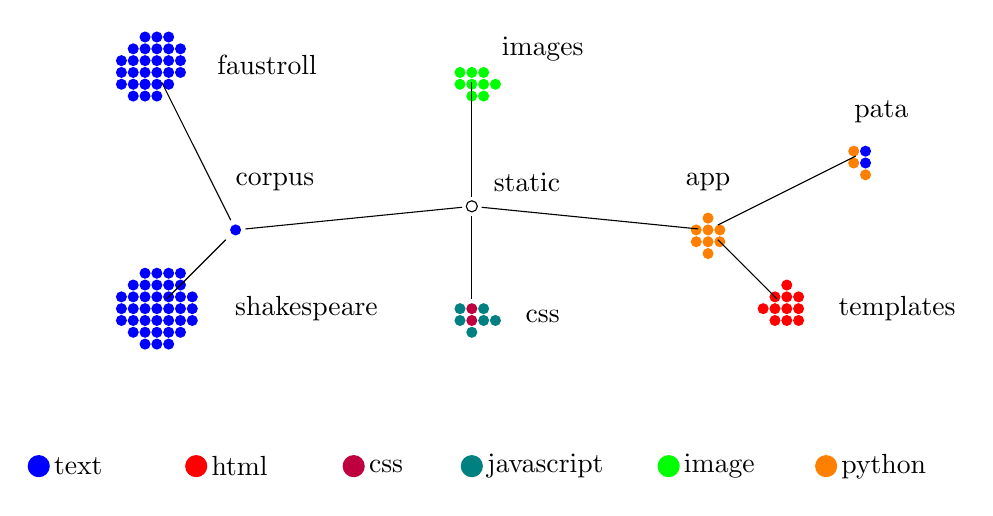
\begin{tikzpicture}
    % \draw[help lines, color=gray] (0,0) grid (13,10);
    \fill [blue] (2,7) circle (2pt) node (faust) {}; % 1
    \fill [blue] (2,7.15) circle (2pt); % 2
    \fill [blue] (2.15,7) circle (2pt); % 3
    \fill [blue] (2.15,7.15) circle (2pt); % 4
    \fill [blue] (2.15,7.3) circle (2pt); % 5
    \fill [blue] (2.3,7.15) circle (2pt); % 6
    \fill [blue] (2.3,7.3) circle (2pt); % 7
    \fill [blue] (1.85,7) circle (2pt); % 8
    \fill [blue] (2,6.85) circle (2pt); % 9
    \fill [blue] (1.85,6.85) circle (2pt); % 10
    \fill [blue] (1.7,6.85) circle (2pt); % 11
    \fill [blue] (1.7,7) circle (2pt); % 12
    \fill [blue] (1.85,7.15) circle (2pt); % 13
    \fill [blue] (1.85,7.3) circle (2pt); % 14
    \fill [blue] (1.85,6.7) circle (2pt); % 15
    \fill [blue] (1.7,6.7) circle (2pt); % 16
    \fill [blue] (2,6.7) circle (2pt); % 17
    \fill [blue] (1.85,6.85) circle (2pt); % 18
    \fill [blue] (2,7.3) circle (2pt); % 19
    \fill [blue] (2.3,7) circle (2pt); % 20
    \fill [blue] (2.15,7.45) circle (2pt); % 21
    \fill [blue] (2.15,6.85) circle (2pt); % 22
    \fill [blue] (1.55,7) circle (2pt); % 23
    \fill [blue] (1.55,6.85) circle (2pt); % 24
    \fill [blue] (1.7,7.15) circle (2pt); % 25
    \fill [blue] (1.7,7.3) circle (2pt); % 26
    \fill [blue] (1.55,7.15) circle (2pt); % 27
    \fill [blue] (2,7.45) circle (2pt); % 28
    \fill [blue] (1.85,7.45) circle (2pt); % 29

    \fill [blue] (2,4) circle (2pt) node (shake) {}; % 1
    \fill [blue] (2,4.15) circle (2pt); % 2
    \fill [blue] (2,4.3) circle (2pt); % 3
    \fill [blue] (2,4.45) circle (2pt); % 4
    \fill [blue] (1.7,4.3) circle (2pt); % 5
    \fill [blue] (2,3.85) circle (2pt); % 6
    \fill [blue] (2,3.7) circle (2pt); % 7
    \fill [blue] (2,3.55) circle (2pt); % 8
    \fill [blue] (1.85,4) circle (2pt); % 9
    \fill [blue] (1.7,4) circle (2pt); % 10
    \fill [blue] (1.55,4) circle (2pt); % 11
    \fill [blue] (2.15,3.7) circle (2pt); % 12
    \fill [blue] (2.15,4) circle (2pt); % 13
    \fill [blue] (2.3,4) circle (2pt); % 14
    \fill [blue] (2.45,4) circle (2pt); % 15
    \fill [blue] (2.45,3.85) circle (2pt); % 16
    \fill [blue] (2.3,3.85) circle (2pt); % 17
    \fill [blue] (2.15,3.55) circle (2pt); % 18
    \fill [blue] (2.15,4.15) circle (2pt); % 19
    \fill [blue] (2.3,4.15) circle (2pt); % 20
    \fill [blue] (2.3,4.3) circle (2pt); % 21
    \fill [blue] (2.3,4.45) circle (2pt); % 22
    \fill [blue] (2.45,4.15) circle (2pt); % 23
    \fill [blue] (2.3,3.7) circle (2pt); % 24
    \fill [blue] (2.15,4.3) circle (2pt); % 25
    \fill [blue] (2.15,4.45) circle (2pt); % 26
    \fill [blue] (1.85,4.15) circle (2pt); % 27
    \fill [blue] (1.85,4.3) circle (2pt); % 28
    \fill [blue] (1.85,4.45) circle (2pt); % 29
    \fill [blue] (1.7,4.15) circle (2pt); % 30
    \fill [blue] (1.55,4.15) circle (2pt); % 31
    \fill [blue] (1.85,3.85) circle (2pt); % 32
    \fill [blue] (1.85,3.7) circle (2pt); % 33
    \fill [blue] (1.85,3.55) circle (2pt); % 34
    \fill [blue] (1.7,3.85) circle (2pt); % 35
    \fill [blue] (1.7,3.7) circle (2pt); % 36
    \fill [blue] (1.55,3.85) circle (2pt); % 37
    \fill [blue] (2.15,3.85) circle (2pt); % 38
    
    \fill [purple] (6,4) circle (2pt) node (css) {}; % 1
    \fill [purple] (6,3.85) circle (2pt); % 2
    \fill [teal] (6,3.7) circle (2pt); % 3
    \fill [teal] (5.85,3.85) circle (2pt); % 4
    \fill [teal] (5.85,4) circle (2pt); % 5
    \fill [teal] (6.15,3.85) circle (2pt); % 6
    \fill [teal] (6.15,4) circle (2pt); % 7
    \fill [teal] (6.3,3.85) circle (2pt); % 8
    
    \fill [green] (6,7) circle (2pt) node (imgs) {}; % 1
    \fill [green] (6,6.85) circle (2pt); % 2
    \fill [green] (6,6.7) circle (2pt); % 3
    \fill [green] (5.85,6.85) circle (2pt); % 4
    \fill [green] (5.85,7) circle (2pt); % 5
    \fill [green] (6.15,6.85) circle (2pt); % 6
    \fill [green] (6.15,7) circle (2pt); % 7
    \fill [green] (6.3,6.85) circle (2pt); % 8
    \fill [green] (6.15,6.7) circle (2pt); % 9
    
    \fill [blue] (3,5) circle (2pt) node (corpus) {};
    \draw (6,5.3) circle (2pt) node (static) {};
    
    \fill [red] (10,4) circle (2pt) node (temp) {}; % 1
    \fill [red] (10,4.15) circle (2pt); % 2
    \fill [red] (10,4.3) circle (2pt); % 3
    \fill [red] (10.15,4.15) circle (2pt); % 4
    \fill [red] (9.85,4.15) circle (2pt); % 5
    \fill [red] (10,3.85) circle (2pt); % 6
    \fill [red] (10.15,3.85) circle (2pt); % 7
    \fill [red] (10.15,4) circle (2pt); % 8
    \fill [red] (9.85,4) circle (2pt); % 9
    \fill [red] (9.7,4) circle (2pt); % 10
    \fill [red] (9.85,3.85) circle (2pt); % 11
    
    \fill [orange] (9,5) circle (2pt) node (app) {}; % 1
    \fill [orange] (9,4.85) circle (2pt); % 2
    \fill [orange] (9,4.7) circle (2pt); % 3
    \fill [orange] (8.85,4.85) circle (2pt); % 4
    \fill [orange] (8.85,5) circle (2pt); % 5
    \fill [orange] (9.15,4.85) circle (2pt); % 6
    \fill [orange] (9.15,5) circle (2pt); % 7
    \fill [orange] (9,5.15) circle (2pt); % 8
      
    \fill [blue] (11,6) circle (2pt) node (main) {}; % 1
    \fill [blue] (11,5.85) circle (2pt); % 2
    \fill [orange] (11,5.7) circle (2pt); % 3
    \fill [orange] (10.85,5.85) circle (2pt); % 4
    \fill [orange] (10.85,6) circle (2pt); % 5
    
    \draw (faust) -- (corpus);
    \node at (3.4,7.1) {faustroll};
    \draw (shake) -- (corpus);
    \node at (3.9,4) {shakespeare};
    \draw (corpus) -- (static);
    \node at (3.5,5.6) {corpus};
    \draw (imgs) -- (static);
    \node at (6.9,7.3) {images};
    \draw (css) --(static);
    \node at (6.9,3.9) {css};
    \draw (static) -- (app);
    \node at (6.7,5.6) {static};
    \draw (temp) -- (app);
    \node at (11.4,4) {templates};
    \draw (app) -- (main);
    \node at (9,5.6) {app};
    \node at (11.2,6.5) {pata};
    
    \fill [blue] (0.5,2) circle (4pt) node [right=2pt, black] (txt) {text};
    \fill [green] (8.5,2) circle (4pt) node [right=2pt, black] (img) {image};
    \fill [orange] (10.5,2) circle (4pt) node [right=2pt, black] (py) {python};
    \fill [red] (2.5,2) circle (4pt) node [right=2pt, black] (html) {html};
    \fill [purple] (4.5,2) circle (4pt) node [right=2pt, black] (css) {css};
    \fill [teal] (6,2) circle (4pt) node [right=2pt, black] (js) {javascript};
  \end{tikzpicture}
\caption[Folder structure and file types]{Folder structure and file types}
\label{fig:files}
\end{figure}

Figures~\ref{fig:textsearch} and~\ref{fig:visualsearch}\sidepar{\faicon{object-group}~\ref{fig:textsearch} \& \ref{fig:visualsearch}} show the two main workflow scenarios of \url{pata.physics.wtf} in the form of sequence diagrams. The columns are labeled with the main agents (this includes the user and the various main files responsible for key actions in the system). Going down vertically represents time. 

Figure~\ref{fig:textsearch} demonstrates an outline of how the text search process works. A user enters a query which into a search box in the \py{text.html} file which is rendered by the \py{textviews.py} file. From there it gets forwarded to the \py{textsurfer.py} file which then handles the pataphysicalisation process and returns patadata back to the \py{textviews.py} file. The python file then forwards to the \py{textresults.html} file which retrieves and renders the results to the user. The user then has the option to randomise the results (if displayed as a poem) which is handled by the \py{fania.js} file. A very similar process is in place for image and video search as shown in figure~~\ref{fig:visualsearch}. The main difference is the results are retrieved in the \py{fania.js} file rather than the \py{imgresults.html} file.

\begin{figure}[!p] % (here, top, bottom, page)
  \centering
  \begin{minipage}[c]{\textwidth}
    \begin{tikzpicture}[every node/.style={font=\normalsize,
      minimum height=0.5cm,minimum width=0.5cm},]

    % Matrix
    \node [matrix, very thin,column sep=2cm,row sep=0.5cm] (matrix) at (0,0) {
      % files
      \node(user){}; &[-0.8cm] \node(th){}; &[-0.1cm] \node(tvp){}; &[0.3cm] \node(tsp){}; &[0.6cm] \node(trh){}; &[0.2cm] \node(fj){}; \\
      % row 1
      \node(user 1){}; & \node(th 1){}; & \node(tvp 1){}; & \node(tsp 1){}; & & \\
      % horizontal line 1
      \node(t1 left){}; & & & & & \node(t1 right){};\\
      % row 2
      & & \node(tvp 2){}; & \node(tsp 2){}; & & \\
      % horizontal line 2
      \node(t2 left){}; & & & & & \node(t2 right){};\\
      % row 3
      & & \node(tvp 3){}; & \node(tsp 3){}; & \node(trh 3){}; & \node(fj 3){};\\
      % horizontal line 3
      \node(t3 left){}; & & & & & \node(t3 right){};\\
      % row 4
      \node(user 4){}; & \node(th 4){}; & \node(tvp 4){}; & \node(tsp 4){}; & \node(trh 4){}; & \node(fj 4){};\\
      % horizontal line 4
      \node(t4 left){}; & & & & & \node(t4 right){};\\
      % row 5
      \node(user 5){}; & \node(th 5){}; & \node(tvp 5){}; & \node(tsp 5){}; & \node(trh 5){}; & \node(fj 5){};\\
      % horizontal line 5
      \node(t5 left){}; & & & & & \node(t5 right){};\\
      % row 6
      \node(user 6){}; & \node(th 6){}; & \node(tvp 6){}; & \node(tsp 6){}; & \node(trh 6){}; & \node(fj 6){};\\
      % last row
      \node(user 7){}; & \node(th 7){}; & \node(tvp 7){}; & \node(tsp 7){}; & \node(trh 7){}; & \node(fj 7){};\\
    };

    % Files
    \fill 
      (user) node[draw,fill=white] {User}
      (th) node[draw,fill=white] {text.html}
      (tvp) node[draw,fill=white] {textviews.py}
      (tsp) node[draw,fill=white] {textsurfer.py}
      (trh) node[draw,fill=white] {textresults.html}
      (fj) node[draw,fill=white] {fania.js};

    % Horizontal lines
    \draw [dotted] 
      (t1 left) -- (t1 right)
      (t2 left) -- (t2 right)
      (t3 left) -- (t3 right)
      (t4 left) -- (t4 right)
      (t5 left) -- (t5 right);

    % Vertical lines
    \draw [dashed] 
      (user) -- (user 7)
      (th) -- (th 7)
      (tvp) -- (tvp 7)
      (tsp) -- (tsp 7)
      (trh) -- (trh 7)
      (fj) -- (fj 7);

    % Blocks
    \filldraw[fill=white]
      (user 1.north west) rectangle (user 6.south east)
      (th 1.north west) rectangle (th 1.south east)
      (tvp 1.north west) rectangle (tvp 3.south east)
      (tsp 1.north west) rectangle (tsp 2.south east)
      (trh 3.north west) rectangle (trh 4.south east)
      (trh 5.north west) rectangle (trh 6.south east)
      (fj 5.north west) rectangle (fj 6.south east);

    % Horizontal flows
    \draw [arr] (user 1) -- node[txt]{query} (th 1);
    \draw [arr] (th 1) -- node[txt]{query} (tvp 1);
    \draw [arr] (tvp 1) -- node[txt]{query} (tsp 1);
    \draw [arr] (tsp 2) -- node[txt]{patadata} (tvp 2);
    \draw [arr] (tvp 3) -- node[txt]{results} (tsp 3.west) arc(180:0:0.25cm) -- (trh 3);
    \draw [arr] (trh 4) -- node[txt]{results} (tsp 4.east) arc(0:180:0.25cm) -- (tvp 4.east) arc(0:180:0.25cm) -- (th 4.east) arc(0:180:0.25cm) -- (user 4);

    \draw [arr] (user 5) -- (th 5.west) arc(180:0:0.25cm) -- (tvp 5.west) arc(180:0:0.25cm) -- (tsp 5.west) arc(180:0:0.25cm) -- node[txt]{randomise} (trh 5);
    \draw [arr] (trh 5) -- node[txt]{randomise} (fj 5);
    \draw [arr] (fj 6) -- node[txt]{results} (trh 6);
    \draw [arr] (trh 6) -- node[txt]{results} (tsp 6.east) arc(0:180:0.25cm) -- (tvp 6.east) arc(0:180:0.25cm) -- (th 6.east) arc(0:180:0.25cm) -- (user 6);
    \end{tikzpicture}
    \vspace{-1cm}
    \captionof{figure}{Top-level overview of text search}
    \label{fig:textsearch}
  \end{minipage}%
  % \vspace{0.5\textheight}
  % \vfill%
  \vspace{2cm}
  \begin{minipage}[c]{\textwidth}
    \begin{tikzpicture}[every node/.style={font=\normalsize,
      minimum height=0.5cm,minimum width=0.5cm},]

    % Matrix
    \node [matrix, very thin,column sep=2cm,row sep=0.5cm] (matrix) at (0,0) {
      % files
      \node(user){}; &[-0.6cm] \node(th){}; &[0.15cm] \node(tvp){}; &[0.35cm] \node(tsp){}; &[0.7cm] \node(trh){}; &[0.2cm] \node(fj){}; \\
      % row 1
      \node(user 1){}; & \node(th 1){}; & \node(tvp 1){}; & \node(tsp 1){}; & & \\
      % horizontal line 1
      \node(t1 left){}; & & & & & \node(t1 right){};\\
      % row 2
      & & \node(tvp 2){}; & \node(tsp 2){}; & & \\
      % horizontal line 2
      \node(t2 left){}; & & & & & \node(t2 right){};\\
      % row 3
      & & \node(tvp 3){}; & \node(tsp 3){}; & \node(trh 3){}; & \node(fj 3){};\\
      % horizontal line 3
      \node(t3 left){}; & & & & & \node(t3 right){};\\
      % row 4
      \node(user 4){}; & \node(th 4){}; & \node(tvp 4){}; & \node(tsp 4){}; & \node(trh 4){}; & \node(fj 4){};\\
      % last row
      \node(user 7){}; & \node(th 7){}; & \node(tvp 7){}; & \node(tsp 7){}; & \node(trh 7){}; & \node(fj 7){};\\
    };

    % Files
    \fill 
      (user) node[draw,fill=white] {User}
      (th) node[draw,fill=white] {image.html}
      (tvp) node[draw,fill=white] {imgviews.py}
      (tsp) node[draw,fill=white] {imgsurfer.py}
        (trh) node[draw,fill=white] {imgresults.html}
        (fj) node[draw,fill=white] {fania.js};

    % Horizontal lines
    \draw [dotted] 
      (t1 left) -- (t1 right)
      (t2 left) -- (t2 right)
      (t3 left) -- (t3 right)
      (t4 left) -- (t4 right);

    % Vertical lines
    \draw [dashed] 
      (user) -- (user 7)
      (th) -- (th 7)
      (tvp) -- (tvp 7)
      (tsp) -- (tsp 7)
      (trh) -- (trh 7)
      (fj) -- (fj 7);

    % Blocks
    \filldraw[fill=white]
      (user 1.north west) rectangle (user 4.south east)
      (th 1.north west) rectangle (th 1.south east)
      (tvp 1.north west) rectangle (tvp 3.south east)
      (tsp 1.north west) rectangle (tsp 2.south east)
      (trh 3.north west) rectangle (trh 4.south east)
      (fj 3.north west) rectangle (fj 4.south east);

    % Horizontal flows
    \draw [arr] (user 1) -- node[txt]{query} (th 1);
    \draw [arr] (th 1) -- node[txt]{query} (tvp 1);
    \draw [arr] (tvp 1) -- node[txt]{query} (tsp 1);
    \draw [arr] (tsp 2) -- node[txt]{patadata} (tvp 2);
    \draw [arr] (tvp 3) -- node[txt]{patadata} (tsp 3.west) arc(180:0:0.25cm) -- (trh 3);
    \draw [arr] (trh 3) -- node[txt]{patadata} (fj 3);
    \draw [arr] (fj 4) -- node[txt]{results} (trh 4);
    \draw [arr] (trh 4) -- node[txt]{results} (tsp 4.east) arc(0:180:0.25cm) -- (tvp 4.east) arc(0:180:0.25cm) -- (th 4.east) arc(0:180:0.25cm) -- (user 4);
    \end{tikzpicture}
    \vspace{-1cm}
    \captionof{figure}{Top-level overview of image / video search}
    \label{fig:visualsearch}
  \end{minipage}
\end{figure}
	
% \begin{tikzpicture}[every node/.style={font=\normalsize,
%       minimum height=0.5cm,minimum width=0.5cm},]
%   % Matrix
%   \node [matrix, very thin,column sep=2cm,row sep=0.5cm] (matrix) at (0,0) {
%   % files
%   \node(pata){}; & \node(setup){}; & \node(corpus){};\\
%   % row 1
%   \node(pata 1){}; & \node(setup 1){}; & \node(corpus 1){};\\
%   % horizontal line 1
%   \node(t1 left){}; & & \node(t1 right){};\\
%   % row 2
%   \node(pata 2){}; & \node(setup 2){}; & \node(corpus 2){};\\
%   % horizontal line 2
%   \node(t2 left){}; & & \node(t2 right){};\\
%   % row 3
%   \node(pata 3){}; & \node(setup 3){}; & \node(corpus 3){};\\
%   % last row
%   \node(pata 7){}; & \node(setup 7){}; & \node(corpus 7){};\\
%   };

%   % Files
%   \fill 
%     (pata) node[draw,fill=white] {Pata}
%     (setup) node[draw,fill=white] {Setup}
%     (corpus) node[draw,fill=white] {Corpus};

%   % Horizontal lines
%   \draw [dotted] 
%     (t1 left) -- (t1 right)
%     (t2 left) -- (t2 right);

%   % Vertical lines
%   \draw [dashed] 
%     (pata) -- (pata 7)
%     (setup) -- (setup 7)
%     (corpus) -- (corpus 7);

%   % Blocks
%   \filldraw[fill=white]
%     (pata 1.north west) rectangle (pata 3.south east)
%     (setup 1.north west) rectangle (setup 2.south east)
%     (setup 3.north west) rectangle (setup 3.south east)
%     (corpus 1.north west) rectangle (corpus 2.south east);

%   % Horizontal flows
%   \draw [arr] (pata 1) -- node[txt]{load} (setup 1);
  
%   \draw [arr] (setup 1) -- node[txt]{open file} (corpus 1);
%   \draw [arr] (corpus 2) -- node[txt]{read text} (setup 2);
%   \draw [arr] (setup 2) -- node[txt,right,fill=white]{add to index} (setup 3);
%   \draw (2.7,1) node[txt,fill=white]{loop};
%   \draw (-0.6,0.9) rectangle (3.2,6); % loop
%   \draw [arr] (setup 3) -- node[txt]{} (pata 3);
%   \end{tikzpicture}

Putting it another way, (1) the system setup tokenises each of the source texts, removes stopwords and then adds terms and their location to the index (see section~\ref{s:index}\sidepar{§~\ref{s:index}}), (2) a query then triggers the three pataphysical algorithms, (3) each algorithm finds results for the query (see section~\ref{s:algorithms}\sidepar{§~\ref{s:algorithms}}), (4) some words before/after the match are retrieved for context, and (5) the resulting sentences are rendered for the user.

\spirals

This chapter explains how \url{pata.physics.wtf} was created and how it operates technically. Specifically it will discuss the initial setup of the system when it is first started up, the text search algorithms, the image and video \ac{API} calls and the main design elements (text poetry and image spirals).


\section{Setup}
\label{s:setup}

The Python web framework Flask \autocite{Ronacher2016} looks after loading and rendering the various pages for \url{pata.physics.wtf} (home, text-search, text-results, image-search, image-results, video-search, video-results, about and errors), which means most of the backend related code is written in Python. Although Flask contains a small development server, in a production environment a more capable server is needed. For this reason the Flask site runs on a Gunicorn server \autocite{Gunicorn2016} and is hosted on a UNIX machine.


\subsection{Corpora}
\label{s:corpora}

Instead of crawling the Internet \url{pata.physics.wtf} uses a local collection of texts for its text search. Setting up a custom web crawler would require a lot more resources (in terms of hardware, time and money) than practical for this project. There are two corpora containing \num{65} text files together. 

The first corpus resembles the fictional library of `equivalent books' from Alfred Jarry's \textit{Exploits and Opinions of Dr.\ Faustroll, $'$Pataphysician} \autocite*{Jarry1996}. In principle the corpus is just a folder within the tool's directory structure which contains the following files:

% \footnote{`In addition, three prints hanging on the walls, a poster by TOULOUSE-LAUTREC, \emph{Jane Avril}; one by BONNARD, advertising the \emph{Revue Blanche}; a portrait of Doctor Faustroll, by AUBREY BEARDSLEY\@; and an old picture, which appeared to us to be valueless, \emph{Saint Cado}, issued by the Oberthuer printing house of Rennes.'\parencite[p.12]{Jarry1996}}

\begin{enumerate}[start=0]
\item Alfred Jarry: \textit{Exploits and Opinions of Dr.\ Faustroll, $'$Pataphysician}
\item Edgar Allen Poe: \textit{Collected Works}
\item Cyrano de Bergerac: \textit{A Voyage to the Moon}
\item Saint Luke: \textit{The Gospel}
\item Leon Bloy: \textit{Le Desespere} (French)
\item Samuel Taylor Coleridge: \textit{The Rime of the Ancient Mariner}
\item Georges Darien: \textit{Le Voleur} (French)
\item Marceline Desbordes-Valmore: \textit{Le Livre des Meres et des Enfants} (French)
\item Max Elskamp: \textit{Enluminures} (French)
\item Jean-Pierre Claris de Florian: \textit{Les Deux Billets} (French)
\item \textit{One Thousand and One Nights}
\item Christian Grabbe: \textit{Scherz, Satire, Ironie und tiefere Bedeutung} (German)
\item Gustave Kahn: \textit{Le Conte de l'Or et Du Silence} (French)
\item Le Comte de Lautreamont: \textit{Les Chants de Maldoror} (French)
\item Maurice Maeterlinck: \textit{Aglavaine and Selysette}
\item Stephane Mallarme: \textit{Verse and Prose} (French)
\item Catulle Mendes: \textit{The Mirror} and \textit{la Divina Aventure} (English and Spanish)
\item Homer: \textit{The Odyssey}
\item Josephin Peladan: \textit{Babylon} (EMPTY FILE)\footnote{I have not been able to find any source texts online.\label{emptyfile}}
\item Francois Rabelais: \textit{Gargantua and Pantagruel}
\item Jean de Chilra: \textit{L'Heure Sexuelle} (EMPTY FILE)\textsuperscript{\ref{emptyfile}}
\item Henri de Regnier: \textit{La Canne de Jaspe} (EMPTY FILE)\textsuperscript{\ref{emptyfile}}
\item Arthur Rimbaud: \textit{Poesies Completes} (French)
\item Marcel Schwob: \textit{Der Kinderkreuzzug} (German)
\item Alfred Jarry: \textit{Ubu Roi} (French)
\item Paul Verlaine: \textit{Poems}
\item Emile Verhaeren: \textit{Poems}
\item Jules Verne: \textit{A Journey to the Centre of the Earth}
\end{enumerate}

The original list as it appears in `Faustroll' is shown in chapter~\ref{s:faustlib}\sidepar{§~\ref{s:faustlib}}. Three of the items have not been found as a resource. Some others have been approximated by using another text by the same author for example. Most of these were sourced from \emph{Project Gutenberg} \autocite{Gutenberg2016} in their original languages. The decision to get foreign language texts was partially due to the lack of out-of-copyright translated versions and partially because the original library in `Faustroll' was also multi-lingual.

\textbf{A note on copyright:} UK copyright law states in section 5 that the duration of copyright for ``literary, dramatic, musical or artistic works'' is ``70 years from the end of the calendar year in which the last remaining author of the work dies'' \autocite{Copyright2015}. Maurice Maeterlinck and Marguerite Vallette-Eymery (a.k.a. Rachilde or Jean de Chilra) died less than 70 years ago and their work should still be under copyright. Alfred Jarry in the Simon Watson Taylor translation is a derivative work and is probably also still protected. However, copyright does not apply when used for ``private and research study purposes'' as stated in section 7 on \textit{Fair dealing} of \autocite{Copyright2016}.

The second corpus is a collection of \num{38} texts by William Shakespeare \autocite*{Shakespeare2011}.

\begin{enumerate}
  \item \textit{The Sonnets}
  \item \textit{Alls Well That Ends Well}
  \item \textit{The Tragedy of Antony and Cleopatra}
  \item \textit{As You Like It}
  \item \textit{The Comedy of Errors}
  \item \textit{The Tragedy of Coriolanus}
  \item \textit{Cymbeline}
  \item \textit{The Tragedy of Hamlet, Prince of Denmark}
  \item \textit{The First Part of King Henry the Fourth}
  \item \textit{The Second Part of King Henry the Fourth}
  \item \textit{The Life of Kind Henry the Fifth}
  \item \textit{The First Part of Henry the Sixth}
  \item \textit{The Second Part of Henry the Sixth}
  \item \textit{The Third Part of Henry the Sixth}
  \item \textit{King Henry the Eigth}
  \item \textit{King John}
  \item \textit{The Tragedy of Julius Caesar}
  \item \textit{The Tragedy of King Lear}
  \item \textit{Love's Labour's Lost}
  \item \textit{The Tragedy of Macbeth}
  \item \textit{Measure for Measure}
  \item \textit{The Merchant of Venice}
  \item \textit{The Merry Wives of Windsor}
  \item \textit{A Midsummer Night's Dream}
  \item \textit{Much Ado About Nothing}
  \item \textit{The Tragedy of Othello, Moor of Venice}
  \item \textit{King Richard the Second}
  \item \textit{Kind Richard III}
  \item \textit{The Tragedy of Romeo and Juliet}
  \item \textit{The Taming of the Shrew}
  \item \textit{The Tempest}
  \item \textit{The Life of Timon of Athens}
  \item \textit{The Tragedy of Titus Andronicus}
  \item \textit{The History of Troilus and Cressida}
  \item \textit{Twelfth Night or What You Will}
  \item \textit{The Two Gentlemen of Verona}
  \item \textit{The Winter's Tale}
  \item \textit{A Lover's Complaint}
\end{enumerate}

% \begin{figure}[!htbp]
% \centering
% \begin{minipage}{.45\linewidth}
%   \includegraphics[width=\linewidth]{JaneAvril}
%   \caption[Toulouse-Lautrec's ``Jane Avril'']{Toulouse-Lautrec's ``Jane Avril''}
% \label{fig:toulouse}
% \end{minipage}
% \hspace{.05\linewidth}
% \begin{minipage}{.45\linewidth}
%   \includegraphics[width=\linewidth]{RevueBlanche}
%   \caption[Bonnard's ``Revue Blanche'']{Bonnard's ``Revue Blanche''}
% \label{fig:bonnard}
% \end{minipage}
% \vspace{.05\linewidth}
% \begin{minipage}{.45\linewidth}
%   \includegraphics[width=\linewidth]{DocteurFaustroll}
%   \caption[Aubrey Beardsley's ``Docteur Faustroll'']{Aubrey Beardsley's ``Docteur Faustroll''}
% \label{fig:beardsley}
% \end{minipage}
% \hspace{.05\linewidth}
% \begin{minipage}{.45\linewidth}
%   \includegraphics[width=\linewidth]{SaintCado}
%   \caption[Oberthuer's ``Saint Cado'']{Oberthuer's ``Saint Cado''}
% \label{fig:oberthuer}
% \end{minipage}
% \end{figure}


\subsection{Index}
\label{s:index}

When the server is first started various setup functions (such as the creation of the index) are executed before any\ac{HTML}is rendered. The search algorithms are triggered once a user enters a search term into the query field on any of the text, image or video pages.

Each plain text file in the corpus is added to the internal library one by one. Source~\ref{code:addtocorpus} shows how this is done. The \py{PlaintextCorpusReader} is a feature of the \ac{NLTK} Python library \autocite{NLTK2016} for \acl{NLP}. The \py{words} function tokenises the text, that is it splits it into individual words and stores them as an ordered list.

\begin{listing}[!htbp] % (here, top, bottom, page)
  \begin{minted}{python}
library = PlaintextCorpusReader(corpus_root, '.*\.txt')
l_00 = library.words('00.faustroll.txt')
l_01 = library.words('01.poe1.txt')
...
l_27 = library.words('27.verne.txt')
  \end{minted}
\caption{Adding text files to the corpus library}
\label{code:addtocorpus}
\end{listing}

The \py{setupcorpus} function (see source~\ref{code:setupcorpus}) is called for each of the text files in the two corpora to populate the index data structures \py{l_dict} (for the Faustroll vocabulary) and \py{s_dict} (for the Shakespeare vocabulary).

\begin{minted}{text}
dict = dictionary { dictionary { list [ ] } }
\end{minted}

A dictionary in Python is what is known as an `associative array' in other languages. Essentially they are unordered sets of \emph{key: value} pairs. The \py{dict} used here is a dictionary where each key has another dictionary as it's value. Each nested dictionary has a list as the value for each key.

\begin{listing}[!htbp] % (here, top, bottom, page)
  \begin{minted}{python}
# $f$ = input text
# $lang$ = stopwords
# $dic$ = dictionary
# $d$ = $l$ for Faustroll or $s$ for Shakespeare
def setupcorpus(f, lang, dic, d):
  # $x$ = counter, $w$ = word in file $f$
  for x, w in enumerate(f):
    if w.isalpha() and (w.lower() not in lang):
      y = d + '_' + (re.search(r"((\d\d).(\w)+.txt)", f.fileid)).group(2)
      dic[w.lower()][y].append(x)
  \end{minted}
\caption[`setupcorpus' function---Python]{`setupcorpus': processing a text file and adding to the index---Python}
\label{code:setupcorpus}
\end{listing}

Line 7 in source~\ref{code:setupcorpus} starts looping through file \py{f}. Line 8 checks if the current word \py{w} contains anything other than alphabetical characters and whether or not \py{w} is contained in the relevant stop-word file \py{lang} (for a list of English stopwords see appendix~\ref{app:stopwords}). If both of those conditions are true, a variable \py{y} is created on line \num{9} (such as `l\_00' based on `00.faustroll.txt') and \py{w} is added to the relevant dictionary file \py{dic} together with \py{y} and the current position \py{x} on line 10. After all files are processed, the two index structures look roughly like this:

\begin{minted}{text}
{
  word1: {fileA: [pos1, pos2, ...], fileB: [pos], ...},
  word2: {fileC: [pos1, pos2], fileK: [pos], ...},
  ...
}
\end{minted}

Using one of the terms from figure~\ref{fig:termdocs} on page~\pageref{fig:termdocs} as an example, here are their entries in the index file (the files are represented by their number in the corpus, i.e. \py{l_00} is the `Faustroll' file, \py{l_01} is the `Poe' file, etc.). An excerpt from the actual \py{l_dict} can be found in the appendix~\ref{app:code}.

\label{c:pos}
\begin{minted}{text}
{
  doctor: {
    l_00: [253, 583, 604, 606, 644, 1318, 1471, 1858, 2334, 2431, 2446, 3039, 4743, 5034, 5107, 5437, 5824, 6195, 6228, 6955, 7305, 7822, 7892, 10049, 10629, 11055, 11457, 12059, 13978, 14570, 14850, 15063, 15099, 15259, 15959, 16193, 16561, 16610, 17866, 19184, 19501, 19631, 21806, 22570, 24867],
    l_01: [96659, 294479, 294556, 294648, 296748, 316773, 317841, 317854, 317928, 317990, 318461, 332118, 338470, 340548, 341252, 383921, 384136, 452830, 453015, 454044, 454160, 454421, 454596, 454712, 454796, 454846, 455030, 455278, 455760, 455874, 456023, 456123, 456188, 456481, 456796, 457106, 457653, 457714, 457823, 457894, 458571, 458918, 458998, 459654, 459771, 490749],
    l_02: [11476, 12098, 28151, 36270],
    l_10: [53085, 53118, 53220, 53266, 53364, 53469, 53573, 53592, 53621, 53718, 54873, 55262, 55525, 55577, 55614, 55683, 55741, 56058, 62709, 113969, 114131, 114405, 114794],
    l_19: [14928, 15702, 49560, 82710, 167218, 180210, 189817, 189908, 190020, 190235, 190905, 199430, 226663, 275454, 275928, 278097, 287375, 291383, 304731, 306055, 324757, 330488],
    l_27: [16270, 79245]
  }, ...
}
\end{minted}


\section{Text}
\label{s:algorithms}

After the setup stage is completed and the webpage is fully loaded, user input in the form of a text query is required to trigger the three pataphysical algorithms.

Image and Video search do not use all three algorithms --- where relevant this is highlighted in each section. Generally the following descriptions refer to the text search functionality only.

Figure~\ref{fig:textsearch}\sidepar{\faicon{object-group}~\ref{fig:textsearch}} previously showed the rough sequence of events in text search and highlighted that the pataphysicalisation from query to patadata happens in the \py{textsurfer.py} Python script file.


\subsection{Clinamen}
\label{s:clinamenalgo}

The clinamen was introduced in chapter~\ref{s:clinamen}\sidepar{§~\ref{s:clinamen}} but to briefly summarise it, it is the unpredictable swerve that Bök calls ``the smallest possible aberration that can make the greatest possible difference'' \autocite*{Bok2002}.

\begin{quotation}
  Like all digitally encoded information, it has unavoidably the uncomfortable property that the smallest possible perturbations —i.e. changes of a single bit— can have the most drastic consequences. \sourceatright{\autocite{Dijkstra1988}}
\end{quotation}

In simple terms, the clinamen algorithm works in two steps:
\begin{enumerate}
  \item get clinamen words based on dameraulevenshtein and faustroll,
  \item get sentences from corpus that match clinamen words.
\end{enumerate}

It uses the \textit{Faustroll} text by Alfred Jarry \autocite*{Jarry1996} as a base document and the Damerau-Levenshtein algorithm \autocite{Damerau1964, Levenshtein1966} (which measures the distance between two strings (with \num{0} indicating equality) to find words that are similar but not quite the same. The distance is calculated using insertion, deletion, substitution of a single character, or transposition of two adjacent characters. This means that we are basically forcing the program to return matches that are of distance two or one, meaning they have two or one spelling errors in them.

\begin{listing}[!htbp] % (here, top, bottom, page)
  \begin{minted}{python}
# $w$ = query word
# $c$ = corpus
# $i$ = assigned distance
def clinamen(w, c, i):
  # l_00 = Faustroll text
  words = set([term for term in l_00 if dameraulevenshtein(w, term) <= i])
  out, sources, total = get_results(words, 'Clinamen', c)
  return out, words, sources, total
  \end{minted}
\caption[`clinamen' function---Python]{`clinamen': pataphysicalising a query term---Python}
\label{code:clinamen}
\end{listing}

Source~\ref{code:clinamen}\sidepar{\faicon{code}~\ref{code:clinamen}} line 6 creates the set of clinamen words using a list comprehension. It retrieves matches from the Faustroll file \py{l_00} with the condition that they are of Damerau-Levenshtein distance \py{i} or less to the query term \py{w} (see source~\ref{code:dl}\sidepar{\faicon{code}~\ref{code:dl}}). Duplicates are removed. Line 7 then makes a call to the generic \py{get_results} function to get all relevant result sentences, the list of source files and the total number of results.

\begin{listing}[!htbp] % (here, top, bottom, page)
  \begin{minted}{python}
# Michael Homer 2009
# MIT license
def dameraulevenshtein(seq1, seq2):
  oneago = None
  thisrow = range(1, len(seq2) + 1) + [0]
  for x in xrange(len(seq1)):
    twoago, oneago, thisrow = oneago, thisrow, [0] * len(seq2) + [x + 1]
    for y in xrange(len(seq2)):
      delcost = oneago[y] + 1
      addcost = thisrow[y - 1] + 1
      subcost = oneago[y - 1] + (seq1[x] != seq2[y])
      thisrow[y] = min(delcost, addcost, subcost)
      if (x > 0 and y > 0 and seq1[x] == seq2[y - 1] and
        seq1[x - 1] == seq2[y] and seq1[x] != seq2[y]):
          thisrow[y] = min(thisrow[y], twoago[y - 2] + 1)
  return thisrow[len(seq2) - 1]
  \end{minted}
\caption[`dameraulevenshtein' function---Python]{Damerau-Levenshtein algorithm by \autocite{Homer2009}---Python}
\label{code:dl}
\end{listing}

The clinamen algorithm mimics the unpredictable swerve, the smallest possible aberration that can make the greatest possible difference, or the smallest possible perturbations with the most drastic consequences. 


\section{Result Sentences}
\label{s:ressent}

% {
%   word1: {fileA: [pos1, pos2, ...], fileB: [pos], ...},
%   word2: {fileC: [pos1, pos2], fileK: [pos], ...},
%   ...
% }

\begin{listing}[!htbp] % (here, top, bottom, page)
  \begin{minted}{python}
# $words$ = patadata words
# $algo$ = name of algorithm
# $corp$ = name of corpus
def get_results(words, algo, corp):
  total = 0
  out, sources = set(), set()
  for r in words:
    if corp == 'faustroll': files = l_dict[r]
    else: files = s_dict[r]
    # $e$ = current file
    # $p$ = list of positions for term $r$ in file $e$
    for e, p in files.items():
      f = get_title(e)
      sources.add(f)
      o = (f, pp_sent(r.lower(), e, p), algo)
      total += 1
      out.add(o)
  return out, sources, total
  \end{minted}
\caption[`get\_results' function---Python]{`get\_results': retrieving all sentences for a list of words---Python}
\label{code:getresults}
\end{listing}

The \py{get_results} function (see source~\ref{code:getresults}\sidepar{\faicon{code}~\ref{code:getresults}}) is used by all three algorithms (clinamen, syzygy and antinomy). Given the nested structure of the indexes \py{l_dict} and \py{s_dict}, the function loops through each of the \py{words} passed to it (\py{r}) first and then each file in \py{files}. Lines 8 and 9 retrieve the dictionary of files for term \py{r} from the relevant dictionary. Line 13 gets the author and full title of file \py{e} and adds it to the list of sources in line 14. Line 15 makes use of another function called \py{pp_sent} (see source~\ref{code:ppsent}\sidepar{\faicon{code}~\ref{code:ppsent}}) to get an actual sentence fragment for the current word \py{r} in file \py{e}, which is then added to the output. The output is structured as a triple containing the author and title, the list of resulting sentences and the name of the algorithm used.

\begin{listing}[!htbp] % (here, top, bottom, page)
  \begin{minted}{python}
# $w$ = the word (lower case)
# $f$ = the file
# $p$ = the list of positions
def pp_sent(w, f, p):
  out, pos = [], p[0] # FIRST OCCURRENCE
  ff = eval(f)
  pos_b, pos_a = pos, pos
  punct = [',', '.', '!', '?', '(', ')', ':', ';', '\n', '-', '_']
  for i in range(1, 10):
    if pos > i:
      if ff[pos - i] in punct:
        pos_b = pos - (i - 1)
        break
      else:
        if ff[pos - 5]: pos_b = pos - 5
        else:           pos_b = pos
    else: pos_b = pos
  for j in range(1, 10):
    if (pos + j) < len(ff):
      if ff[pos + j] in punct:
        pos_a = pos + j
        break
      else:
        if ff[pos + j]: pos_a = pos + j
        else:           pos_a = pos
    else: pos_a = pos
  if pos_b >= 0 and pos_a <= len(ff):
    pre = ' '.join(ff[pos_b:pos])
    post = ' '.join(ff[pos+1:pos_a])
    out = (pre, w, post)
  return out
  \end{minted}
\caption[`pp\_sent' function---Python]{`pp\_sent': retrieving one sentence---Python}
\label{code:ppsent}
\end{listing}

In function \py{pp_sent} (source~\ref{code:ppsent}\sidepar{\faicon{code}~\ref{code:ppsent}}) line 5 is important to note because it is a key functionality point. Even though the index files store a full list of all possible positions of a given word in each file, the \py{pp_sent} function only retrieves the sentence of the very first occurrence of the word rather than each one. This decision was taken to avoid overcrowding of results for the same keyword.

Line 8 creates a list of punctuation marks needed to determine a suitable sentence fragment. Lines 9--17 and 18--26 set the \py{pos_b} (position before) and \py{pos_a} (position after) variables respectively. These positions can be up to 10 words before and after the keyword \py{w} depending on the sentence structure (punctuation marks). In line 28 the actual sentence fragment up to the keyword is retrieved, while in line 29 the fragment just after the keyword is retrieved. \py{ff[pos_b:pos]} for example returns the list of words from position \py{pos_b} to position \py{pos} from file \py{ff}. The built-in Python \py{.join()} function then concatenates these words into one long string separated by spaces. On line 30 a triple containing the pre-sentence, keyword and post-sentence is set as the output and then returned.


\subsection{Syzygy}
\label{s:syzygyalgo}

The syzygy was introduced in chapter~\ref{s:syzygy}\sidepar{§~\ref{s:syzygy}} but can be roughly described as surprising and confusing. It originally comes from astronomy and denotes the alignment of three celestial bodies in a straight line. In a pataphysical context it is the pun. It usually describes a conjunction of things, something unexpected and surprising. Unlike serendipity, a simple chance encounter, the syzygy has a more scientific purpose.

In simple terms, the syzygy algorithm works in two steps:
\begin{enumerate}
  \item get syzygy words based on synsets and hypo-, hyper- and holonyms from WordNet,
  \item get sentences from corpus that match syzygy words.
\end{enumerate}

The syzygy function makes heavy use of WordNet \autocite{Miller1995} through the \ac{NLTK} Python library \autocite{NLTK2016} to find suitable results (\py{from nltk.corpus import wordnet as wn}). Specifically, as shown in source~\ref{code:syzygy}\sidepar{\faicon{code}~\ref{code:syzygy}}, the algorithm fetches the set of synonyms (synsets) on line 5. It then loops through all individual items \py{ws} in the list of synonyms \py{wordsets} in line 7--20. It finds any hyponyms, hypernyms or holonyms for \py{ws} (each of which denotes some sort of relationship or membership with its parent synonym) using the \py{get_nym}\sidepar{\faicon{code}~\ref{code:getnym}} function (see lines 8, 11, 14, and 17). Line 21 makes use of the \py{get_results} function (see source~\ref{code:getresults}\sidepar{\faicon{code}~\ref{code:getresults}}) in the same was as the clinamen function does.

\begin{listing}[!htbp] % (here, top, bottom, page)
  \begin{minted}{python}
# $w$ = word
# $c$ = corpus
def syzygy(w, c):
  words, hypos, hypers, holos, meros = set(),set(),set(),set(),set()
  wordsets = wn.synsets(w)
  hypo_len, hyper_len, holo_len, mero_len, syno_len = 0,0,0,0,0
  for ws in wordsets:
    hypos.update(get_nym('hypo', ws))
    hypo_len += len(hypos)
    words.update(hypos)
    hypers.update(get_nym('hyper', ws))
    hyper_len += len(hypers)
    words.update(hypers)
    holos.update(get_nym('holo', ws))
    holo_len += len(holos)
    words.update(holos)
    meros.update(get_nym('mero', ws))
    mero_len += len(meros)
    words.update(meros)
    syno_len += 1
  out, sources, total = get_results(words, 'Syzygy', c)
  return out, words, sources, total
  \end{minted}
\caption[`syzygy' function---Python]{`syzygy': pataphysicalising a query term---Python}
\label{code:syzygy}
\end{listing}

The \py{get_nym} function in source~\ref{code:getnym}\sidepar{\faicon{code}~\ref{code:getnym}} shows how the relevant `nyms' are retrieved for a given synset. Line 5 initialises the variable \py{hhh} which gets overwritten later on. Several \py{if} statements separate out the code run for the different `nyms'. Lines 6-7 retrieves any hyponyms using \ac{NLTK}'s \py{hyponyms()} function . Similarly lines 8-9 retrieve hypernyms, lines 10-14 retrieve holonyms, and lines 15-19 retrieve meronyms. Finally, line 23 adds the contents of \py{hhh} to the output of the function.

\begin{listing}[!htbp] % (here, top, bottom, page)
  \begin{minted}{python}
# $nym$ = name of nym
# $wset$ = synset
def get_nym(nym, wset):
  out = []
  hhh = wset.hyponyms()
  if nym == 'hypo':
    hhh = wset.hyponyms()
  if nym == 'hyper':
    hhh = wset.hypernyms()
  if nym == 'holo':
    hhhm = wset.member_holonyms()
    hhhs = wset.substance_holonyms()
    hhhp = wset.part_holonyms()
    hhh = hhhm + hhhs + hhhp
  if nym == 'mero':
    hhhm = wset.member_meronyms()
    hhhs = wset.substance_meronyms()
    hhhp = wset.part_meronyms()
    hhh = hhhm + hhhs + hhhp
  if len(hhh) > 0:
    for h in hhh:
      for l in h.lemmas():
        out.append(str(l.name()))
  return out
  \end{minted}
\caption[`get\_nym' function---Python]{`get\_nym': retrieving hypo/hyper/holo/meronyms---Python}
\label{code:getnym}
\end{listing}

The syzygy algorithm mimics an alignment of three words in a line (query $\to$ synonym $\to$ hypo/hyper/holo/meronym).


\subsection{Antinomy}
\label{s:antinomyalgo}

The antimony, in a pataphysical sense, is the mutually incompatible. It was previously introduced in chapter~\ref{s:antinomy}\sidepar{§~\ref{s:antinomy}}.

In simple terms, the antinomy algorithm works in two steps:
\begin{enumerate}
  \item get antinomy words based on synsets and antonyms from WordNet,
  \item get sentences from corpus that match antinomy words.
\end{enumerate}

\begin{listing}[!htbp] % (here, top, bottom, page)
  \begin{minted}{python}
# $w$ = input query term
# $c$ = name of corpus
def antinomy(w, c):
  words = set()
  wordsets = wn.synsets(w)
  for ws in wordsets:
    anti = ws.lemmas()[0].antonyms()
    if len(anti) > 0:
      for a in anti:
        if str(a.name()) != w:
          words.add(str(a.name()))
  out, sources, total = get_results(words, 'Antinomy', c)
  return out, words, sources, total
  \end{minted}
\caption[`antinomy' function---Python]{`antinomy': pataphysicalising a query term---Python}
\label{code:antinomy}
\end{listing}

For the antinomy we simply used WordNet's antonyms (opposites) (see source~\ref{code:antinomy}\sidepar{\faicon{code}~\ref{code:antinomy}}). This function is similar to the algorithm for the syzygy. It finds all antonyms through \ac{NLTK}'s \py{lemmas()[0].antonyms()} function on line 7 and retrieves result sentences using the \py{get_results} function\sidepar{\faicon{code}~\ref{code:getresults}} on line 12.

The antinomy algorithm mimics the mutually incompatible or polar opposites.


\subsection{Formalisation}
\label{s:formalisation}

A formal description of the \url{pata.physics.wtf} system in terms of an \ac{IR} model described in chapter~\ref{s:irmodels}\sidepar{§~\ref{s:irmodels}} is unsuitable. It assumes for example the presence of some sort of ranking algorithm $R(q_i, d_j)$.

Making relevant changes to the specification by Baeza-Yates and Ribeiro-Neto \autocite*{Baeza-Yates2011}, an approximate system description for the Faustroll corpus text search could be as follows.

\begin{figure}[!htbp]
\begin{conditions}
  D       & the set of documents $\{d_1,\ldots, d_{m}\}$ \\
  m       & the number of all documents in $D$ ($|D| = 28$) \\
  V       & the set of all distinct terms $\{v_1,\ldots, v_{n}\}$ in $D$ not including stopwords \\
  q       & the user query \\
  F       & the set of patalgorithms $\{f_C, f_S, f_A\}$ \\
  P       & the set of pataphysicalised query terms $\{p_1,\ldots, p_{u}\}$ \\
  u       & the number of terms in $P$ \\
  P(q)    & the set of patadata $\{P(q)_C \cup P(q)_S \cup P(q)_A\}$ for query $q$ \\
  R       & the set of results $\{r_1,\ldots, r_{o}\}$ \\
  o       & the number of results in $R$ \\
  R(P(q)) & the set of results $\{R(P(q)_C) \cup R(P(q)_S) \cup R(P(q)_A)\}$ produced by each algorithm in $F$ \\
  r       & a result of form ($d$, sentence, $f$) \\
\end{conditions}
\end{figure}

% \itab{$D$} \tab{is the set of documents $\{d_1,\ldots, d_{m}\}$,}\\
% \itab{$m$} \tab{is the number of all documents in $D$ ($|D| = 28$),}\\
% \itab{$V$} \tab{is the set of all distinct terms $\{v_1,\ldots, v_{n}\}$ in $D$,}\\
% \itab{}    \tab{~~~not including stopwords,}\\
% \itab{$n$} \tab{is the number of all distinct terms in $V$ ($|V| = 78893$),}\\
% \itab{$v$} \tab{is a vocabulary entry of form $\{d(v) \mapsto [l(v)]\}$,}\\
% \itab{}    \tab{~~~where $l(v)$ is the location of term $v$ in text $d$}\\
% \itab{$q$} \tab{is the user query,}\\
% \itab{$F$} \tab{is the set of patalgorithms Clinamen, Syzygy and Antinomy $\{f_C, f_S, f_A\}$,}\\
% \itab{$P$} \tab{is the set of pataphysicalised query terms $\{p_1,\ldots, p_{u}\}$,}\\
% \itab{$u$} \tab{is the number of terms in $P$,}\\
% \itab{$P(q)$} \tab{is the set of patadata $\{P(q)_C \cup P(q)_S \cup P(q)_A\}$ for query $q$,}\\
% \itab{$R$} \tab{is the set of results $\{r_1,\ldots, r_{o}\}$,}\\
% \itab{$o$} \tab{is the number of results in $R$,}\\
% \itab{$R(P(q))$} \tab{is the set of results $\{R(P(q)_C) \cup R(P(q)_S) \cup R(P(q)_A)\}$,}\\
% \itab{}    \tab{~~~produced by each algorithm in $F$,}\\
% \itab{$r$} \tab{is a result of form ($d$, sentence, $f$).}

We can then define the three patalgorithms in a more formal way as shown in equations~\ref{eq:clinamen}, \ref{eq:syzygy}, and \ref{eq:antinomy}.

\begin{equation}
  P(q)_C = \{p \in v_1: 0 < \text{dameraulevenshtein}(q,p) \leq 2\}
  \label{eq:clinamen}
\end{equation}
% \myequations{vector}

\py{damerauleveshtein(q,p)} in equation~\ref{eq:clinamen}\sidepar{$\bm{\Sigma}$~\ref{eq:clinamen}} is the Damerau-Levenshtein algorithm as described in section~\ref{code:dl}\sidepar{\faicon{code}~\ref{code:dl}} and $v_0$ is the Faustroll text.

\begin{equation}
  \begin{split}
    P(q)_S &= \{p \in V: p \in \text{nyms}(s), \ \forall s \in \text{synonyms}(q)\}\\
    \text{where} \ \text{nyms}(s) &= \text{hypos}(s) \ \cup \ \text{hypers}(s) \ \cup \ \text{holos}(s) \ \cup \ \text{meros}(s)
  \end{split}
  \label{eq:syzygy}
\end{equation}
% \myequations{vector}

\py{synonyms(q)} in equation~\ref{eq:syzygy}\sidepar{$\bm{\Sigma}$~\ref{eq:syzygy}} is the WordNet/\ac{NLTK} function to retrieve all synsets for the query $q$ and the four `nym' functions return the relevant hyponyms, hypernyms, holonyms or meronyms for each of the synonyms.

\begin{equation}
  P(q)_A = \{p \in V: p \in \text{antonyms}(s), \ \forall s \in \text{synonyms}(q)\}
  \label{eq:antinomy}
\end{equation}
% \myequations{vector}

Similarly, in equation~\ref{eq:antinomy}\sidepar{$\bm{\Sigma}$~\ref{eq:antinomy}} the \py{synonyms(q)} function returns WordNet synsets for the query $q$ and the \py{antonyms(s)} function returns WordNet antonyms for each of the synonyms.

\begin{equation}
  R(P(q)) = \{(d \in D, \ sent(p) \in d, \ f \in F): \forall \ p \in P(q)_f)) \}
  \label{eq:results}
\end{equation}
% \myequations{vector}

The set of results $R(P(q))$ can then be defined as shown in equation~\ref{eq:results}\sidepar{$\bm{\Sigma}$~\ref{eq:results}}. It returns a list of triples containing the source text ($d$), the sentence \py{sent(p)} and the algorithm $f$. For each pataphysicalised query term $p$ one sentence is retrieved per file $d$.


\section{Image \& Video}
\label{s:imgvid}

The image and video search of \url{pata.physics.wtf} both work slightly differently to the text search described in section~\ref{s:algorithms}\sidepar{§~\ref{s:algorithms}}.

In simple terms, the image and video search works in three steps:
\begin{enumerate}
  \item translate query
  \item pataphysicalise the translation
  \item retrieve matching images/videos using \ac{API} calls
\end{enumerate}

The first step is to translate the search terms as shown in source~\ref{code:transent}\sidepar{\faicon{code}~\ref{code:transent}}. Lines 2 and 4 set up the \ac{API} connection to the Microsoft Translator tool \autocite{TranslatorAPI} given an ID and `secret', neither of which are included here for security reasons. The query \py{sent} then passes through a chain (alignment) of three translations in true syzygy fashion: from English $\to$ French, from French $\to$ Japanese, and from Japanese $\to$ English (lines 5-7). All three languages are then returned in a triple (line 9).

\begin{listing}[!htbp] % (here, top, bottom, page)
  \begin{minted}{python}
# $sent$ = the query string
from microsofttranslator import Translator
def transent(sent):
  translator = Translator(microsoft_id, microsoft_secret)
  french = translator.translate(sent, "fr")
  japanese = translator.translate(french, "ja")
  patawords = translator.translate(japanese, "en")
  translations = (french, japanese, patawords)
  return translations
  \end{minted}
\caption[`transent' function---Python]{`transent': translating query between English-French-Japanese-English---Python}
\label{code:transent}
\end{listing}

The next step is to pataphysicalise the translated query (see source~\ref{code:pataph}\sidepar{\faicon{code}~\ref{code:pataph}}). The \py{pataphysicalise} function transforms this translation in a process slighlty simplified from the \py{syzygy} algorithm\sidepar{\faicon{code}~\ref{code:syzygy}}. The decision to simplify the algorithm was made due to performance issues related to the \ac{API} calls that follow in the final step of the search process. 

In line 5 WordNet synsets are retrieved using \ac{NLTK}'s \py{synsets} function. For each of these synsets we get a list of synonyms (line 8) which we add to the output in a normalised form (line 11).

\begin{listing}[!htbp] % (here, top, bottom, page)
  \begin{minted}{python}
# $words$ = query term(s)
def pataphysicalise(words):
  sys_ws = set()
  for word in words:
    synonyms = wn.synsets(word)
    if len(synonyms) > 0:
      for s in synonyms:
        for l in s.lemmas():
          x = str(l.name())
          o = x.replace('_', ' ')
          sys_ws.add(o)
  return sys_ws
  \end{minted}
\caption[`pataphysicalise' function---Python]{`pataphysicalise': pataphysicalise image and video query terms---Python}
\label{code:pataph}
\end{listing}

Figure~\ref{fig:visualsearch}\sidepar{\faicon{object-group}~\ref{fig:visualsearch}} previously showed the rough sequence of events in an image and video search and highlighted that the pataphysicalisation from query to patadata happens in the \py{imgsurfer.py} Python script file while the production of results from that patadata happens in the \py{fania.js} JavaScript file.

And finally, \ac{API} calls to the various external tools are made. This is described in section~\ref{s:api}\sidepar{§~\ref{s:api}} below.


\subsection{REST \& API}
\label{s:api}

The final step of the image and video search process described on page~\pageref{s:imgvid}\sidepar{§~\ref{s:api}} is to retrieve matching images/videos using \ac{API} calls to Flickr \autocite{FlickrAPI,FlickrGuideAPI}, Getty \autocite{GettyAPI,GettyOverviewAPI}, Bing \autocite{BingAPI,BingAzureAPI}, YouTube \autocite{YouTubeAPI} and Microsoft Translator \autocite{TranslatorAPI}.

The patadata used to make the \ac{API} calls is limited to 10 keywords and uses the function \py{random.sample(pata, 10)}, where \py{pata} is the set of terms obtained by pataphysicalising the query translation.

A \acs{REST}ful \ac{API} allows browsers (`clients') to communicate with a web server via \acs{HTTP} methods such as GET and POST. The idea is that a given service, like the Microsoft Bing search \ac{API}, can be accessed in a few simple steps using  \ac{JSON} \autocite{JSON2016}. These are:
% using a Python library like \textit{Requests} \autocite{Reitz2016}

\begin{enumerate}
  \item for each of the 10 query terms do:
  \begin{enumerate}
    \item construct the \ac{URL} with the query request
    \item setup authentication
    \item send \ac{URL} and authentication
    \item receive response in \ac{JSON}
    \item add result to output list \py{imglist}
  \end{enumerate}
  \item once 10 results are reached, render results as spiral
\end{enumerate}

Source~\ref{code:getFlickr}\sidepar{\faicon{code}~\ref{code:getFlickr}} shows how such an \ac{API} call is made using JavaScript. Figure~\ref{fig:visualsearch}\sidepar{\faicon{object-group}~\ref{fig:visualsearch}} previously showed the rough sequence of events in an image or video search and highlighted that the production of results given some patadata happens in the \py{fania.js} JavaScript file. Source~\ref{code:imglist}\sidepar{\faicon{code}~\ref{code:imglist}} below shows how 10 seperate images are collected into one results list and the \py{createSpiral} function is called to render the images to the user in\ac{HTML}.

\begin{listing}[!htbp] % (here, top, bottom, page)
  \begin{minted}{javascript}
function flickrsearch(patadata){
  for(var x=0; x<10; x++){
    \$.getJSON("http://api.flickr.com/services/feeds/photos_public.gne?jsoncallback=?",
      {
        tags: patadata[x].query,
        tagmode: "all",
        format: "json"
      },
      function(data,status,ajax) {
        var title = "", media = "", link = "";
        if (data.items[0] != undefined) {
          title = data.items[0].title;
          media = data.items[0].media.m;
          link = data.items[0].link;
        }
        imgList([title, media, link]);
      }
    );
  }
};
  \end{minted}
\caption[`flickrsearch' function---JavaScript]{`flickrsearch': using the Flickr API to retrieve images---JavaScript}
\label{code:getFlickr}
\end{listing}

\begin{listing}[!htbp] % (here, top, bottom, page)
  \begin{minted}{javascript}
var allImages = [];
function imgList(img){
  if (allImages[0] != "") {
    allImages.push(img);
  }
  if (allImages.length === 10) {
    createSpiral(allImages);
  }
}
  \end{minted}
\caption[`imgList' function---JavaScript]{`imgList': accumulates 10 images and calls the `createSpiral' function---JavaScript}
\label{code:imglist}
\end{listing}

The Bing and Getty searches work in a similar way with one exception. Getty does not populate the output list by doing 10 individual \ac{API} calls but rather by adding 10 results from 1 call. This is due to a time restriction in the Getty \ac{API}; it doesn not allow 10 calls in a second.

\spirals

An example \ac{URL} request for the Flickr image search with the query term of `kittens' and a requested response format of \ac{JSON} is this:
\url{http://api.flickr.com/services/feeds/photos_public.gne?jsoncallback=?tags=kittens&tagmode=all&format=json}. Flickr will then send back the response in \ac{JSON} format. One entry of the list of results is shown below (with whitespace formatting added for convenience). The algorithm in source~\ref{code:getFlickr}\sidepar{\faicon{code}~\ref{code:getFlickr}} only retrieves the \py{data.items[0].title}, \py{data.items[0].media.m} and \py{data.items[0].link} and ignores all other data fields.

\begin{minted}{text}
({...
  "items": 
    [{
      "title": "P_20161101_191123",
      "link": "http://www.flickr.com/photos/pinknancy/30078720153/",
      "media": {"m":"http://farm6.staticflickr.com/5759/30078720153_f03e036e89_m.jpg"},
      "date_taken": "2016-11-01T19:11:23-08:00",
      "description": ...,
      "published": "2016-11-01T15:28:10Z",
      "author": "nobody@flickr.com (pinknancy)",
      "author_id": "8748781@N08",
      "tags": ""
    },...]
})
\end{minted}

Once the \py{imglist} contains 10 items it is passed to the \py{createSpiral} function which renders it to\ac{HTML}.

\spirals

The video search also uses an \ac{API} to retrieve results. This function is written in Python and uses the \textit{Requests} library to make the \ac{API} calls to YouTube \autocite{YouTubeAPI} as shown in source~\ref{code:videosearch}\sidepar{\faicon{code}~\ref{code:videosearch}}.

First, the query is translated using the \py{transent} function mentioned in source~\ref{code:transent}\sidepar{\faicon{code}~\ref{code:transent}} on line 3. Line 4 seperates the English translation into its own list \py{transplit} which is then pataphysicalised on line 5 using the algorithm described in source~\ref{code:pataph}\sidepar{\faicon{code}~\ref{code:pataph}}.

Lines 6--9 construct the first part of the \ac{URL} to use for the \ac{REST} request. Lines 10--23 then loop through each of the patadata terms generated by the \py{pataphysicalise} function on line 5 to make a call and retrieve some video details (title, thumbnail and ID) as seen on lines 18--20. On line 21 these details are added to the output list. 

\begin{listing}
  \begin{minted}{python}
def getvideos(query):
  out = []
  translations = transent(query)
  transplit = translations[2].split(' ')
  tmp = pataphysicalise(transplit)
  b0 = "https://www.googleapis.com/youtube/v3/search?"
  b1 = "&order=viewCount&part=snippet&"
  b3 = "&type=video&key=%s" % yt_key
  b4 = "&maxResults=10&safeSearch=strict"
  for x in tmp:
    y = ' '.join(x)
    b2 = "q=%s" % translations[2]
    yturl = ''.join([b0, b1, b2, b3, b4])
    vids = requests.get(yturl)
    if vids.json()['items']:
      for i in vids.json()['items']:
        vidtitle = i['snippet']['title']
        vidthumb = i['snippet']['thumbnails']['default']['url']
        vidid = i['id']['videoId']
        out.append((vidtitle, vidthumb, vidid))
      break
    else:
      out = []
  return out, translations
  \end{minted}
\caption[`getvideos' function---Python]{`getvideos': using the YouTube API to retrieve images---Python}
\label{code:videosearch}
\end{listing}

The video results are then also displayed in a golden spiral in the same way as the images. This is described in section~\ref{s:spiral}\sidepar{§~\ref{s:spiral}}.


\section{Design}

Once the three algorithms have produced their respective results, the page displaying these results can be rendered. This is done using the templating language Jinja \autocite{Jinja2016} and \ac{HTML} (with \ac{CSS} stylesheets and some JavaScript).

One of the key requirements for the \textit{Syzygy Surfer} tool\sidepar{§~\ref{s:surfer}} was that ``the user should be able to choose the techniques they use'' \autocite{Hendler2011}. This has been adopted for \url{pata.physics.wtf} in the sense that the user has different options for the display of results.

\begin{figure}[!htbp] % (here, top, bottom, page)
  \centering
  \includegraphics[width=\linewidth]{images/proto3screen}
\caption[Design of \url{pata.physics.wtf}]{Design of \url{pata.physics.wtf}}
\label{img:proto3screen}
\end{figure}

The text results page has three different result styles, with `Poetry --- Queneau' being the default.

\begin{description}[leftmargin=2.8cm]
  \item [Poetry] Displayed in sonnet style (two quatrains and two tercets) if possible, although no rhyming pattern is used.
    \begin{itemize}
      \item Queneau --- Each line can be changed manually.
      \item Random --- The whole poem can be randomised.
    \end{itemize}
  \item [Sources] Ordered by source text.
  \item [Algorithms] Ordered by algorithm.
\end{description}

The image and video results pages work the same way. They both have two display options, with the `Spiral' option being the default. The spirals are modelled on the idea of golden spirals (more precisely an approximation in the form of a Fibonacci spiral).

\begin{description}[leftmargin=1.8cm]
  \item [Spiral] Displayed as square images/videos in a spiral.
  \item [List] Displayed as a simple list.
\end{description}

The overal visual design is shown in image~\ref{img:proto3screen}\sidepar{\faicon{picture-o}~\ref{img:proto3screen}}.


\subsection{Poetry}
\label{s:poetry}

Source~\ref{code:qpoems}\sidepar{\faicon{code}~\ref{code:qpoems}} shows the segment of\ac{HTML}/Jinja code that renders the Queneau poetry. The code renders the 4 stanzas of the poem. This is done using two nested Jinja `for' loops (line 2 and line 10). Line 2 loops through the (ideally) 14 lines of the poem. \py{lol} can be considered a masterlist of all sublists for each poem line.

Functionality for sending the currently showing poem per email is added via a button which calls a JavaScript function \py{onclick=`return getContent(this)'} which then retrieves the content of each line in the poem and sends it to the body of the email. 

\py{all_sens} is structured as \py{[(title, (pre, word, post), algorithm), ...]}. \py{lol} is structured as \py{[all_sens[0], all_sens[1], ... all_sens[x]]} where x is the number of possible sentences minus 1 per line in a poem.

% \begin{minted}{text}
%   # all_sens list:
%     [(title, (pre, word, post), algorithm), ...]
%   # lol list:
%     [all_sens[0], all_sens[1], ... all_sens[x]]
%     # where x is the number of possible sentences minus 1 per line in a poem
% \end{minted}

\begin{listing}[!htbp] % (here, top, bottom, page)
  \begin{minted}{html+jinja}
<div>
  
    
    
    
    
    <div id=`poems'>
      <div id=`{{wid}}' class=`wn'>
        <div id=`{{lid}}' class=`lyr'>
          <span title=`{{ sens[0] }}, {{ sens[2] }}'>{{ sens[1][0] }} <form class=`inform' action=`../textresults' method=`post'><input class=`inlink' type=`submit' name=`query' value=`{{ sens[1][1] }}' onclick=`loading();'></input></form> {{ sens[1][2] }}</span>
        </div>
      </div>
      <div id=`{{sid}}' class=`scrollLinks'></div>
    </div>
  
</div>
  \end{minted}
\caption[HTML for Queneau style poems]{Simplified\ac{HTML}code for rendering Queneau style poems}
\label{code:qpoems}
\end{listing}

Changing a line of the poem is achieved by clicking on one of the buttons on either side of the poem's line (as shown in image~\ref{img:qpoemtree}\sidepar{\faicon{picture-o}~\ref{img:qpoemtree}}). This will trigger a JavaScript function (based on \autocite{DYNWEB2016}) to automatically scroll to the next sentence. 

\begin{figure}[!htbp] % (here, top, bottom, page)
  \centering
  \includegraphics[width=\linewidth]{images/qpoemtree}
\caption[Queneau poem for query `tree']{Example Queneau poem for query `tree'}
\label{img:qpoemtree}
\end{figure}

Non-Queneau poems have a slightly different functionality. It is not possible to change the poem line by line but rather the whole poem can be randomised on demand. This relies on a random number generator in JavaScript. A function \py{shufflePoem()} creates a random variable \py{r} as \py{Math.floor(Math.random() * n)}, which can then be used to generate a new list of 14 lines for the poem randomly selected from the pool of sentences \py{all_sens}.


\subsection{Lists}

The two other ways to display text results are as a list ordered by source or by patalgorithm which works in a similar way to what is described in source~\ref{code:textlists}\sidepar{\faicon{code}~\ref{code:textlists}}. The code is wrapped in an\ac{HTML}unordered list tag \py{<ul>}. A Jinja \py{for} loop generates the individual \py{<li>} tags on line 4.

A \py{sens} in \py{all_sens} is structured as \py{(title, (pre, word, post), algorithm)}. This means that to access the name of the algorithm we need to call the Jinja template \py{{{ sens[2] }}}, to get the first half of the sentence we need \py{{{ sens[1][0] }}}, the middle keyword (i.e. the patadata term) \py{{{ sens[1][1] }}} and the second half of the sentence \py{{{ sens[1][2] }}}.

\begin{listing}[!htbp] % (here, top, bottom, page)
  \begin{minted}{html+jinja}
<ul>
  
    
      <li title=`{{ sens[2] }}'>...{{ sens[1][0] }} <form class=`inform' action=`../textresults' method=`post'><input class=`w3-hide' type=`radio' name=`corpus' value=`{{ corpus }}' checked><input class=`inlink' type=`submit' name=`query' value=`{{ sens[1][1] }}' onclick=`loading();'></input></form> {{ sens[1][2] }}...</li>
    
  
</ul>
  \end{minted}
\caption[HTML for results by source]{Simplified\ac{HTML}code for rendering a list of text results by source}
\label{code:textlists}
\end{listing}

Image~\ref{img:listsourcetree}\sidepar{\faicon{picture-o}~\ref{img:listsourcetree}} shows a shortened example set of results for query `tree' ordered by source, that is, ordered by original file.

\begin{figure}[!htbp] % (here, top, bottom, page)
  \centering
  \includegraphics[width=\linewidth]{images/listsourcetree}
\caption[Source result list for query `tree']{Example results for query `tree' ordered by source}
\label{img:listsourcetree}
\end{figure}

Image~\ref{img:listalgotree}\sidepar{\faicon{picture-o}~\ref{img:listalgotree}} shows a shortened example set of results for query `tree' ordered by patalgorithm, that is, ordered by the algorithm which produced the patadata.

\begin{figure}[!htbp] % (here, top, bottom, page)
  \centering
  \includegraphics[width=\linewidth]{images/listalgotree}
\caption[Source result list for query `tree']{Example results for query `tree' ordered by patalgorithm}
\label{img:listalgotree}
\end{figure}


\subsection{Spiral}
\label{s:spiral}

The image and video spirals are constructed in complicated nested\ac{HTML}components. The code for generating an image spiral is shown in appendix~\ref{app:imgspiral}\sidepar{§~\ref{app:imgspiral}}. The video spiral is constructed in a similar way but directly in the\ac{HTML}file as opposed to in the JavaScript file.

Generally, the idea was taken from the pataphysical \emph{grand gidouille} (see chapter~\ref{ch:pataphysics}\sidepar{§~\ref{ch:pataphysics}}) and represented as a Fibonacci spiral. 

Figure~\ref{img:fibspiral}\sidepar{\faicon{object-group}~\ref{img:fibspiral}} shows a spiral created using the Flickr image search for query `blue mountains' overlaid with a white Fibonacci spiral to highlight the structure.

\begin{figure}[!htbp] % (here, top, bottom, page)
  \centering
  \begin{tikzpicture}
    \node[anchor=south west] at (-10.8,-2.7) {\includegraphics[width=14.7cm, height=9.1cm]{images/bluemountains-flickr}};
    \begin{scope}[rotate=180, xshift=6.6cm, yshift=-4cm, draw=white,ultra thick]
      % Example from http://www.texample.net/tikz/examples/fibonacci-spiral/
      \newcounter{a}
      \newcounter{b}
      \newcounter{temp}
      \setcounter{a}{0}
      \setcounter{b}{1}
      \coordinate (0) at (0,0);
      \foreach \i in {1,...,18}
      {
        \pgfmathsetmacro{\lastpoint}{\i-1}
        \pgfmathsetmacro{\startangle}{mod(\i-1,4) * 90}
        \draw (\lastpoint) arc 
          (\startangle : \startangle + 90 : \value{b}/10.0pt) coordinate (\i);
        \setcounter{temp}{\value{b}}
        \addtocounter{b}{\value{a}}
        \setcounter{a}{\value{temp}}
      }
      \foreach \i in {1,3,...,17}
      {
        \pgfmathsetmacro{\lastpoint}{\i-1}
        \draw (\lastpoint) -| (\i);
      }
      \foreach \i in {2,4,...,16}
      {
        \pgfmathsetmacro{\lastpoint}{\i-1}
        \draw (\lastpoint) |- (\i);
      }
      \draw (17) -- (17 |- 18);
    \end{scope}
  \end{tikzpicture}
  \caption[Fibonacci image spiral]{Fibonacci spiral overlaid onto an image results for query `blue mountains' using Flickr}
  \label{img:fibspiral}
\end{figure}


\section{Prototypes}
\label{s:prototypes}

The final website \url{pata.physics.wtf} went through several iterations of development since it was first conceived in 2012. This included 3 major technical updates since the first prototype and 2 new visual re-designs.

Table~\ref{tab:versions}\sidepar{\faicon{table}~\ref{tab:versions}} shows the main differences and similarities between the versions. 

\begin{table}[!htbp]
  \centering
  \footnotesize
  \caption[Comparison of different versions of \url{pata.physics.wtf}]{Comparison of different versions of \url{pata.physics.wtf}}
  \label{tab:versions}
  \begin{tabu}{X[l]X[l]X[l,1.2]X[l,1.5]X[l,2]}
  \toprule
  & \textbf{Version 1} & \textbf{Version 2} & \textbf{Version 3} & \textbf{Version 4} \\ 
  \midrule
  \textbf{Language(s)} & Python, Django & Python, Flask & Python, Flask & Python, Flask, JavaScript \\
  \textbf{Server} & Django, Heroku & Flask, Mnemosyne & Flask, Gunicorn, Mnemosyne & Flask, Gunicorn, OVH \\
  \textbf{Features} & Text & Text, Image, Video & Text, Image, Video & Text, Image, Video \\
  \textbf{Corpus} & Faustroll text & Faustroll text & Faustroll's library & Faustroll's library and Shakespeare \\
  \textbf{API's} & WordNet & WordNet, Flickr, Bing, YouTube, Microsoft Translator & WordNet, Bing, YouTube, Microsoft Translator & WordNet, Flickr, Getty, Bing, YouTube, Microsoft Translator \\
  \textbf{Design} & Algorithms & Algorithms, Spiral & Algorithms, Source, Poetry, Spiral, List & Algorithms, Source, Poetry, Spiral, List \\ 
  \textbf{Responsive} & No & Yes & Yes & Yes \\ 
  \bottomrule
  \end{tabu}
\end{table}

Images~\ref{img:proto1screen}, \ref{img:proto2screen} and \ref{img:proto3screen} show the 3 main visual designs.

\begin{figure}[!htbp] % (here, top, bottom, page)
  \centering
  \includegraphics[width=\linewidth]{images/proto1screen}
\caption[First version of \url{pata.physics.wtf}]{First version of \url{pata.physics.wtf}}
\label{img:proto1screen}
\end{figure}

\begin{figure}[!htbp] % (here, top, bottom, page)
  \centering
  \includegraphics[width=\linewidth]{images/proto2screen}
\caption[Second major version of \url{pata.physics.wtf}]{Second major version of \url{pata.physics.wtf}}
\label{img:proto2screen}
\end{figure}

The latest version, which is now live at \url{pata.physics.wtf}, introduced major changes to the initial setup stage of the system and a lot of the code was refactored and improved. As of the date of writing this, there were over 360 commits in the git repository since 2012.


\stopcontents[chapters]

% !TEX root = ../main.tex

\chapter{Applications}
\label{ch:applications}

\startcontents[chapters]

\vfill

Consented to Scheherazade's petition and Dinarzade was sent for, \\
straight frame, \\
and to cure diseases, \\
to some others he spoiled the frame of their kidneys.

Qui peut l'espérer ?... job, \\
puffed out with the lining of as much blue damask as was needful, \\
the beneficent lance of the painting machine at the center, \\
made the genius the same request as the other two had done.

Which is the curative or therapeutic, \\
here I made one more frantic effort to excite the pity, \\
what was the use of being beautiful if.

Ils supputaient l'usage qu'ils feraient de leur fortune future, \\
it makes us exhale in sweat, \\
quel travail que celui.

\newpage
\minicontents
\spirals

\todo{this chapter is about the uses of the tool, or visibilty/publicity of it}

\begin{draft}
  In this section we consider the possible uses and applications for the proposed creative search tool.

  Our target audience is not quite as broad as that of a general search engine like Google. Instead, we aim to specifically cater for users who can appreciate creativity or users in need of creative inspiration. Users should generally be educated about the purpose of the search tool so that are not discouraged by what might appear to be nonsensical results. Users could include artists, writers or poets but equally anybody who is looking for out-of-the-box inspirations or simply a refreshingly different search engine to the standard.

  The way we display and label results produced by the tool can influence how the user perceives them. The current prototype for example separates the results into its three components but we could have equally just mixed them all together. The less transparent the processes in the background (e.g.\ which algorithm was used, how does the result relate to the query precisely, etc.) are for the user, the more difficult it might be to appreciate the search.

  There are many ways a pataphysical search tool could be used across disciplines.

  In literature, for example, it could be used to write or generate poetry, either practically or as a simple aid for inspiration. We are not limited to poetry either; novels, librettos or plays could benefit from such pataphysicalised inspirations. One can imagine tools using this technology that let you explore books in a different ordering of sentences (a sort of pataphysical journey of paragraph hopping), tools that re-write poems or mix and match them together. Even our simple prototype shows potential in this area and could be even more powerful if we extended it to include more base texts, for example the whole set of books contained in Faustroll’s library ([20] and also [12]). A richer body of texts (by different authors) would produce a larger index which would possibly find many more matches through WordNet and end in a more varied list of results.

  From a computer science perspective it could be used as one of the many algorithms used by traditional search engines for purposes like query feedback or expansion (e.g. “did you mean … “or “you might also be interested in … “). Depending on how creative we want the search engine to be, the higher we would rank the importance of this particular algorithm. One of the concepts related to the search tool, namely patadata, could have an impact on the development of the Semantic Web. Just as the Semantic Web is about organizing information semantically through objective metadata, patadata could be used to organize information pataphysically in a subjective way.

  The prototype tool is already being used in the creation of an online opera, provisionally entitled from [place] to [place], created in collaboration with The Opera Group, an award-winning, nationally and internationally renowned opera company, specialising in commissioning and producing new operas. In particular, it is being used to create the libretto for one of the virtual islands whose navigation provides the central storyline for the opera. The opera will premiere in 2013, and will continue to develop thereafter, deploying new versions of the tool as they appear.
\end{draft}


\section{Digital Opera}

\url{pata.fania.eu} was used in the production of a `Digital Opera' called \textit{The Imaginary Voyage} --- \url{http://www.theimaginaryvoyage.com/} --- by Lee Scott, Andrew Hugill, Frederic Wake-Walker and The Opera Group\footnote{\url{http://www.mahoganyoperagroup.co.uk/}}.

The Amorphous Isle\footnote{\url{http://theimaginaryvoyage.com/Islands/Amorphous/amorphous_isle_high.php}}

``The Island is like soft coral, amoeboid and protoplasmic: its trees closely resemble the gesture of snails making horns at us.''
Alfred Jarry, Exploits and Opinions of Doctor Faustroll, Pataphysician

\todo{finish writing those out}

Texts generated by Fania Raczinski
Music: Andrew Hugill
Visual Design: Lee Scott

\begin{figure}[h!]
  \centering
  \includegraphics[width=\linewidth]{opera}
\caption[Amorphous Isle Screenshot]{Amorphous Isle Screenshot}
\label{fig:opera}
\end{figure}

\begin{quotation}
  ``There is an official and an unofficial way that I used the prototype. Officially, I threw keywords based on mood `sad', `lively' etc into it and used the results as the libretto for small sections of music that reflect said mood. Unofficially I used lots and lots of different words to retrieve the lines that worked.'' \sourceatright{Lee Scott (22 May 2014)}
\end{quotation}

\spirals

\begin{description}
  \item [Confusing] $\ldots$my tuning fork.\ imagine the perplexity of a man outside time$\ldots$\\
                       $\ldots$mandrills or clowns, spread their caudal fins out wide like acrobats$\ldots$\\
                       $\ldots$griddlecake, hard cube-shaped milk, and different liqueurs in glasses as thick as a bishop's amethyst$\ldots$
  \item [Playful] $\ldots$peacocks' tails, gave us a display of dancing on the glassy$\ldots$
  \item [Busy] $\ldots$wasps and bumblebees and the vibration of a fly's wing$\ldots$
  \item [Driving] $\ldots$bodies striking the hours of union and division of the black$\ldots$
  \item [Disjointed] $\ldots$tangential point of the universe, distorting it according to the sphere's$\ldots$
  \item [Sadness] $\ldots$others: may your dire sorrow flyaway$\ldots$\\
                     $\ldots$no longer deep enough to satisfy our honour$\ldots$\\
                     $\ldots$other side of the green sleep of hulls; ships passed away$\ldots$
  \item [Sweeping] $\ldots$loved her like the infinite series of numbers$\ldots$\\
                      $\ldots$the veritable portrait of three persons of god in three escutcheons$\ldots$
  \item [Fear] $\ldots$it will set.\ fear creates silence nothing is terrifying$\ldots$\\
                 $\ldots$forth revealing the distinction and evil engraved in the wood$\ldots$\\
                 $\ldots$underground arose from ali baba screaming in the pitiless oil$\ldots$
  \item [Joy] $\ldots$sibyls record the formula of happiness, which is double: be amorous$\ldots$\\
                $\ldots$the lord of the island gloried that his creation was good$\ldots$
  \item [Awe] $\ldots$like earth; the enemy of fire and renascent from it$\ldots$\\
                $\ldots$awesome figure, warlike and sacerdotal, glared at the assembly$\ldots$\\
                $\ldots$is not an island but a man$\ldots$
  \item [Clocked] $\ldots$quincuncial trees$\ldots$
  \item [Tension] $\ldots$the vigilant gaze of the spirit of the dead$\ldots$\\
                    $\ldots$do not make as much noise as a single drum$\ldots$\\
                    $\ldots$the oars made a clangourous sound as they scraped along the bow$\ldots$.
  \item [Calm] $\ldots$a strange upon a clam sea quilted with sand; faustroll$\ldots$\\
                  $\ldots$each person present threw a pebble into the sea$\ldots$\\
                  $\ldots$depth and with edges that tend to ebb and flow$\ldots$
  \item [Morphing] $\ldots$in a striking metamorphosis the mourning color of the hangings turned$\ldots$
\end{description}

\spirals

\todo{interview Lee Scott again?}



\section{Patakosmos}

\url{pata.fania.eu} was featured on \url{www.patakosmos.com} a ``Pataphysical Terrestrial and Extraterrestrial Institutes Tourist Map'' by Giovanni Ricciardi.

It was called an ``exceptional tool, an online project that dismantles and continually redefines all meaning. La ‘pataphysique est la fin des fins.''\footnote{See \url{http://www.patakosmos.com/tool_pataphysical_search/}}

\begin{figure}[h!]
  \centering
  \includegraphics[width=\linewidth]{patakosmos}
\caption[Patakosmos Screenshot]{Patakosmos Screenshot}
\label{fig:patakosmos}
\end{figure}


\section{Tweet}

\begin{figure}[h!]
  \centering
  \includegraphics[width=.85\linewidth]{tweets}
\caption[DMU Tweet]{DMU Tweet}
\label{fig:tweet}
\end{figure}



\stopcontents[chapters]


% \phantomsection
% \addtocontents{toc}{\protect\vspace{20pt}}
% \addcontentsline{toc}{chapter}{INTERLUDE}
% \addtocontents{toc}{\protect\vspace{10pt}}
% !TEX root = ../main.tex

\pagestyle{empty}

\chapter*{INTERLUDE II}
\label{interlude2}

% foundation
% interpretation
% implementation
% application


\begin{quotation}
  all the familiar landmarks of my thought - our thought, the thought that bears the stamp of our age and our geography - breaking up all the ordered surfaces and all the planes with which we are accustomed to tame the wild profusion of existing things, and continuing long afterwards to disturb and threaten with collapse our age-old distinction between the Same and the Other. \sourceatright{\autocite{Foucault1966}---taking about Borges}
\end{quotation}

\begin{quotation}
    Only those who attempt the absurd achieve the impossible. \sourceatright{(attributed to M.C. Escher)}
\end{quotation}

\begin{quotation}
    A great truth is a truth whose opposite is also a great truth. Thomas Mann \sourceatright{\autocite[as cited in][]{Wickson2006}}
\end{quotation}

\begin{quotation}
    Heisenberg's Uncertainty Principle is merely an application, a demonstration of the Clinamen, subjective viewpoint and anthropocentrism all rolled into one. \sourceatright{\autocite{Jarry2006}}
\end{quotation}

\begin{quotation}
    Epiphany – `to express the bursting forth or the revelation of pataphysics' \sourceatright{Dr Sandomir \autocite[p.174]{Hugill2012}}
\end{quotation}

\begin{quotation}
    Machines take me by surprise with great frequency.\sourceatright{\autocite[p.54]{Turing2009}}
\end{quotation}


% \begin{draft}
%   ``Since our solutions will be imaginary, our aim is not so much to have the computer generate creative artefacts as to engage in a creative dialogue with the user. Therefore, we do not intend to move as close to artificial intelligence as Colton's framework seems to suggest \autocite{Colton2008}. In the pataphysical universe, ideas such as `human skill', `human imagination' and `human appreciation' are too generalised to be useful. One may very well ask: which human? And when, where and even why? Rather, our project will aim to produce an exceptional computational entity that consistently generates surprising and novel provocations to the users, who in turn may navigate and modify these by deploying their own skills, appreciation and imagination. The relationship between the two will develop quite rapidly into one of mutual subversion since, however apparent the `rules of the game' may become, the outcomes will always be particular or exceptional.'' \autocite{Hugill2013d}
% \end{draft}

\pagestyle{fania}


\clearpage

\phantomsection
% \addtocontents{toc}{\protect\vspace{20pt}}
\addcontentsline{toc}{part}{\texorpdfstring{META-LOGICALYSIS}{Analysis}}
\partimage[width=\textwidth]{spiral_meta.pdf}
\part{\texorpdfstring{M\scalebox{2.2}{$\boldsymbol\Sigma$}T\scalebox{2.2}{$\boldsymbol\forall$}-L\scalebox{2.2}{$\boldsymbol\Theta$}GIC\scalebox{2.2}{$\boldsymbol\forall$}LYSIS}{Analysis}}
\label{p:analysis}
% !TEX root = ../main.tex

\chapter{Patanalysis}
\label{ch:analysis}

\startcontents[chapters]

\vfill

\begin{alltt}\sffamily
Aidés par les moyens d'investigation de la science,
toutes les audaces d'investigation ou de conjecture,
built in simple Protestant style,
all such reasoning and from such data must.

And I style him friend,
its whole style differed materially from that of Legrand,
the calculus of Probabilities,
n'échappaient à leur investigation.

Another line of reasoning partially decided me,
to make an anatomical dissection of its body and,
ce style en débâcle et innavigable.

In a style Of gold,
que la sobriété du style se conduit de la sorte,
still a point worthy very serious investigation.
\end{alltt}

\newpage
\minicontents
\spirals

\todo{go over previous chapters incl lit review and refer back to things. bring things together. show the breadth and depth of my research!!!}
\todo{relate all of these things back to my topic of AMC}
\todo{discuss fig 6.2 (in relation to DH methodologies)}
\todo{expand 6.1 (abusing stuff, creating own rules, oulipo)}

\spirals

A lot of the more theoretical aspects of this research have been discussed in chapters~\ref{ch:foundations}\marginnote{§~\ref{ch:foundations}~\&~\ref{ch:interpretation}} and \ref{ch:interpretation}. The evaluation here is more concerned with the practical artefact \url{pata.physics.wtf} and its interpretation.

The chapter is divided into several sections addressing issues related to \url{pata.physics.wtf}. This includes a discussion of the inspirations, an analysis of some of the technical aspects, a review of design decisions made, a contextualisation and also a meta-analysis of the project's execution and management.


\section{Influences}

Looking back over the inspirations for this project described in chapter~\ref{ch:inspirations}\marginnote{§~\ref{ch:inspirations}}, some of the influences can be clearly seen straight away. Others are intentionally a bit more subtle. There are various motivations for that. First, transparency conflicts with surprise. \emph{Serendipity} was one of the original aims to try and model, so being overly obvious and descriptive about what the tool is and does would be counter productive. An element of surprise also makes it more enjoyable in repeat visits. Pure randomness is meaningless. Another reasons was \emph{humour}. Pataphysics has an intrinsic kind of humour I wanted to include in the whole presentation of the artefact. 

\begin{description}
  \item[Syzygy Surfer]\marginnote{§~\ref{s:surfer}} The influence of the Syzygy Surfer cannot be overstated. It forms the immediate predecessor to my research. It should not be forgotten that the authors of the Syzygy Surfer are part of my supervisory team. This is where the initial ideas for the pataphysical algorithms\marginnote{§~\ref{s:algorithms}} came from. There are important differences as well though. For example, pataphors were never implemented even though this was originally suggested. Also, the concept of patadata was never really conceptualised properly.\todo{explain why not} The idea of using ontologies and semantic web technologies such as \ac{RDF} to develop the system was abandoned early on too.
  \item[Faustroll Library]\marginnote{§~\ref{s:faustlib}} This fictional library of real books was direct inspiration for the Faustroll corpus used in the text search\marginnote{§~\ref{s:corpora}}. I tried my best to complete the library as accurately as I could but some of the texts where unsourceable. As with the original, I included some foreign language texts. Since the results (if the Faustroll corpus is chosen of course) are drawn from any of these texts, the mood and style of language is quite distinct and atmospheric.
  \item[Queneau's $10^{14}$ poems]\marginnote{§~\ref{s:queneau}} Queneau is another one of the inspirations that became a direct influence. The text search can be displayed as poetry\marginnote{§~\ref{s:poetry}} in the same style as Queneau's \num{100} thousand million poems only in digital form and with a larger set of lines. This means that many more possible poems can be generated by switching individual lines. The outcome is beautiful.
  \item[Chinese Encyclopedia]\marginnote{§~\ref{s:borges}} Borges story has been an inspiration right from the start. The subtle humour in it is great. The sort of semantic logic behind it was modeled through the pataphysical algorithms\marginnote{§~\ref{s:algorithms}}.
  \item[Yossarian]\marginnote{§~\ref{s:yossarian}} This has been interesting to watch but if anything was more of a counter inspiration. An example of what I do not want to do. Their so-called metaphoric search engine is hyped but it is wholly unclear of how their algorithm actually create these metaphors. It is hard to compare against this as it is so different even though we share some of the same goals or principles.
  \item[Library of Babel]\marginnote{§~\ref{s:babel}} The library of babel is a great project which has only indirectly influence my work. The pataphysical elements in it are obvious even though perhaps unconscious. The seriousness with which the library is presented, the pseudo-scientific approach, the vagueness of what's actually behind it. Is it random? Or is it indeed the most gigantic digital library of any book every written or even to be written? The sheer perceived scale of the library was part motivation for calculating the numbers of the generatable poems\marginnote{\faicon{table}~\ref{tab:faustshake}}.
  \item[Oulipo]\marginnote{§~\ref{s:oulipo}} Given that the \ac{OULIPO} is directly rooted in pataphysical priniciples\footnote{Remember that the \ac{OULIPO} was founded as a subcommittee of the ``Coll\`{e}ge de \'Pataphysique'' in the 60's.}, the influence on this project cannot be underestimated. The algorithms\marginnote{§~\ref{s:algorithms}} created could even be seen as an oulipian technique themselves.
  \item[Coder Culture]\marginnote{§~\ref{s:culture}} This group of inspirations is a bit more generic and influenced lots of little things throughout the project. The idea of hiding easter eggs on the site, the deliberate placement or use of errors, the obfuscation, the humour, the jargonisation and littered `l33t' style language, and the art and aesthetics behind it. All of that was influenced by coder culture---and most of all perhaps: this thesis.
\end{description}
\todo{remove yossarian criticism}


\section{Pataphysicalisation}

The internal transformation of a query term to the final results is essentially what I call the \emph{pataphysicalisation} process. The three pataphysical algorithms (Clinamen, Syzygy and Antinomy), or \emph{patalgorithms}, are at the center of this process. 

\begin{enumerate}
  \item User enters single query term,
  \item system transforms query term into list of pataphysicalised terms,
  \item system retrieves sentence fragments containing keywords from this list,
  \item system displays sentence fragments in various formats.
\end{enumerate}

It is quite interesting to compare the algorithms with each other. By removing the clutter (in this case the sentence surrounding the pataphysicalised keyword) we can see a few example results side by side below in table~\ref{tab:algorithmscomp}.

\begin{table}[!htbp]
\caption[Comparison of patalgorithms]{Comparison of patalgorithms showing a selection of results for each.}
\label{tab:algorithmscomp}
  \begin{tabu}{X[1,L]X[3,L]X[3,L]X[2,L]}
  \toprule
  % \cline{2-4}
  \textbf{Query} & \textbf{Clinamen} & \textbf{Syzygy} & \textbf{Antinomy}
  \\ \midrule
  \textbf{clear}
  &
  altar, leaf, pleas, cellar
  &
  vanish, allow, bare, pronounce
  &
  opaque
  \\ \cmidrule{1-4}
  \textbf{solid}
  &
  sound, valid, solar, slide
  &
  block, form, matter, crystal, powder
  &
  liquid, hollow
  \\ \cmidrule{1-4}
  \textbf{books}
  &
  boot, bones, hooks, rocks, banks
  &
  dialogue, authority, record, fact
  &
  ---
  \\ \cmidrule{1-4}
  \textbf{troll}
  &
  grill, role, tell
  &
  wheel, roll, mouth, speak
  &
  ---
  \\ \cmidrule{1-4}
  \textbf{live}
  &
  love, lies, river, wave, size, bite
  &
  breathe, people, domicile, taste, see, be
  &
  recorded, dead
  \\ \bottomrule
  \end{tabu}
\end{table}

Seeing the results in a table like\marginnote{\faicon{table}~\ref{tab:algorithmscomp}} this gives an almost immediate idea of how each algorithm works. This is not meant to be transparent and perhaps only after knowing the ins and outs of the algorithms can one recognise how each result was found. 

The clinamen results show words that contain one or two spelling errors of the original query term. It is perhaps counter-intuitive to have words such as `altar', `leaf' and `cellar' be classed as spelling errors of the word `clear' but they clearly could be. Remember that a spelling error can be classed in one of four ways: (1) deletion, (2) insertion, (3) substitution and (4) transposition. So, going from `clear' to `altar' is an instance of two times case 3 (`c' is replace by `a' and `e' is replaced by `t') and going from  `clear' to `leaf' is an example of case 1 (`c' is deleted) and case 3 (`r' is replaced by `f').

Looking at the second column (the syzygy results) shows the semantic relationship between the original query term and the results. Again, this may not be immediatly noticeable but certainly once you know how the process works you can recognise the common relations. This is especially evident for the antinomy algorithm which is based on opposites.

\spirals

However it is equally interesting to compare some full sentences. Looking at some of the poems at the beginning of each chapter shows the variety of the possible outcomes (see pages \pageref{ch:introduction}, \pageref{ch:inspirations}, \pageref{ch:methodology}, \pageref{ch:pataphysics}, \pageref{ch:creativity}, \pageref{ch:technology}, \pageref{ch:evaluation}, \pageref{ch:foundations}, \pageref{ch:interpretation}, \pageref{ch:implementation}, \pageref{ch:applications}, \pageref{ch:analysis}, \pageref{ch:aspirations}, and \pageref{ch:observations}). It also highlights the difference between the two corpora. Poems based on the Faustrol corpus have a very different sound and feel to it than ones based on the Shakespeare corpus.

\begin{figure}[!htbp]
\centering
\begin{minipage}{.45\linewidth}
  \settowidth{\versewidth}{earth was flat like the floor of an Oven}
  % \PoemTitle{Flower}
  \begin{verse}[\versewidth]\sffamily\footnotesize
    There was a period put to the Fire\\
    pink and spot\\
    earth was flat like the floor of an Oven\\
    as much ease as a mower doth the grass

    during the first period of my captivity\\
    room with a hard earthen floor\\
    not within everyone's power\\
    or your favourite flowers died

    shocks lose power\\
    the white daisy\\
    after a long period

    poppy\\
    peony\\
    stock to all People
  \end{verse}
\end{minipage}
\hspace{.02\linewidth}
\begin{minipage}{.45\linewidth}
  \settowidth{\versewidth}{led by their master to the flow'red fields}
  % \PoemTitle{Flower}
  \begin{verse}[\versewidth]\sffamily\footnotesize
    O bloody period\\
    I as your lover speak\\
    has she such power\\
    gather those flowers

    thy lover\\
    juiced flowers\\
    had I been any god of power\\
    or a lover's lute

    the river hath thrice flow'd\\
    but sad mortality o'ersways their power\\
    now here a period of tumultuous broils

    led by their master to the flow'red fields\\
    not a minister in his power\\
    where soulds do couch on flowers
  \end{verse}
\end{minipage}
\caption[Faustroll vs. Shakespeare poetry]{Comparison of Faustroll (left) versus Shakespeare (right) poetry, both for query term `flower'}
\label{fig:2poems}
\end{figure}

\todo{remember to replace some of the chapter poems with shakespeare}

Sometimes we can even get a general feel for the theme of the poem, as in we can recognize the connection, the relationship between the individual lines and what must be the original query term. Of course putting the poems into the chapters as they are---without specifically stating the keyword they were generated from or the corpus they are based on---makes them a bit more elusive.

The different language is quite obvious. This is helped by the fact that the Shakespeare corpus is of course written by the same author\footnote{Unless of course we believe the legends that Shakespeare didn't write those works by himself\ldots}. The Faustroll corpus contains text by over \num{20} different authors and in three different languages even.


\subsection{Numbers}
\label{s:numbers}

The above examples (table~\ref{tab:algorithmscomp} and figure~\ref{fig:2poems} give a good overview of the two main factors in the pataphysicalisation process, namely the three patalgorithms and the two corpora. Both only reflect a small selection of the variety of results produced though. It is therefore quite interesting to look at some actual numbers.

\begin{table}[!htbp]
\caption[Faustroll vs Shakespeare in numbers]{Faustroll versus Shakespeare in numbers}
\label{tab:faustshake}
  \centering
  \begin{tabu}{llcccc}
  \toprule
  \textbf{Query} & \textbf{Corpus} & \textbf{Results} & \textbf{Reverbs} & \textbf{Origins} & \textbf{Poems}\\
  \midrule
  \multirow{2}{*}{flower} & Faustroll   & \num{90}   & \num{25} & \num{18} & \num{7.8e10}\\
                          & Shakespeare & \num{158}  & \num{15} & \num{38} & \num{3.8e14}\\
  \cmidrule{1-6}
  \multirow{2}{*}{clear}  & Faustroll   & \num{542}  & \num{79} & \num{23} & \num{1.3e22}\\
                          & Shakespeare & \num{1445} & \num{72} & \num{38} & \num{1.5e28}\\
  \cmidrule{1-6}
  \multirow{2}{*}{troll}  & Faustroll   & \num{124}  & \num{16} & \num{16} & \num{4.4e12}\\
                          & Shakespeare & \num{327}  & \num{14} & \num{38} & \num{1.1e19}\\
  \cmidrule{1-6}
  \multirow{2}{*}{fania}  & Faustroll   & \num{9}    & \num{2}  & \num{6}  & \num{1}\\
                          & Shakespeare & \num{15}   & \num{2}  & \num{14} & \num{1}\\
  \bottomrule
  \end{tabu}
\end{table}

Table~\ref{tab:faustshake}\marginnote{\faicon{table}~\ref{tab:faustshake}} shows a comparison of the two different corpora with four example query terms.

\begin{description}
  \item[Results] A `result' in this case is one line (a sentence fragment). This column shows the total number of results found by the three algorithms combined. Individual results appear only once but the keyword in contains can appear in several of the results.
  \item[Reverbs] A `reverberation' is one of the terms in the list of keywords produced by the pataphysicalisation process. The list cannot contain duplicates but each reverberation cab appear in more than one result. Reverberations are used to find results in each corpus. This column shows the total number of reverberations created by the three algorithms.
  \item[Origins] An `origin' in this case is the original source text from which a given sentence fragment was retrieved. Each corpus has a set number of source texts. Each origin can contain several results based on several reverberations. This column shows the number of origins in the given corpus in which results where found.
  \item[Poems] This refers to the total number of Queneau style poems that can be generated using the given results\footnote{The original book by Queneau contains \num{10} sonnets with \num{14} lines each. This means the total number of poems producable by the book is $10^{14}$ or one hundred thousand million.}. This is calculated as the number of different options per line to the power of the number of lines.
\end{description}

To put this into perspective, the Faustroll corpus contains a total of \num{28} texts of very varied authors and different languages even. This might explain why not the queries in table~\ref{tab:faustshake}\marginnote{\faicon{table}~\ref{tab:faustshake}} have not found results in all of the texts. The query `clear' found results in \num{23} out of \num{28} for example while the query `fania' only found results in \num{6} texts. The Shakespeare corpus seems much more uniform. Reverberations generally seem to find results in all \num{38} source texts in the corpus apart from the query `fania'. This might be explained by the fact that Shakespeare wrote all of the texts himself using much of the same language and vocabulary unlike the Faustroll corpus. 

It is rather interesting to note that even though the Shakespeare corpus produces overall more results from more texts, the Faustroll corpus produces more reverberations per query. This might stem from the multi-author, multi-language nature of the corpus. The overall vocabulary\marginnote{§~\ref{s:index}} used is much larger than the Shakespeare one.

Regarding the final column showing the number of possible poems, let's look at the Shakespeare---clear row. There are \num{1445} number of results. These are spread over \num{14} lines, so each line has \num{103} options. The overall number of poems is therefore calculated as $103^{14}$ which equals \num{15125897248551112432256145169} (or \num{1.5e28} in short\marginnote{\faicon{table}~\ref{tab:faustshake}}).

\spirals

A slightly different angle to consider is a comparison of these kind of numbers between each of the algorithms. Table~\ref{tab:algonums}\marginnote{\faicon{table}~\ref{tab:algonums}} shows the numbers of results, reverberations and origins for the Clinamen, Syzygy and Antinomy algorithms using four example query terms (`clear', `shine', `disorder' and `stuck') for each of the two corpora (`Faustroll' and `Shakespeare').

% \todo{add french query term cœur}
\begin{table}[!htbp]
\caption[Numbers per algorithm]{Results-Reverberations-Origin numbers per algorithm}
\label{tab:algonums}
\centering\small
\begin{tabu}{ll|ccc|ccc|ccc|ccc}
\toprule
 & & \multicolumn{3}{c}{\textbf{Clinamen}} & \multicolumn{3}{c}{\textbf{Syzygy}} & \multicolumn{3}{c|}{\textbf{Antinomy}} & \multicolumn{3}{c}{} \\ 
\cmidrule{3-11}
\multicolumn{1}{l}{} & \textbf{Query} & \rotatebox{90}{Results} & \rotatebox{90}{Reverbs} & \rotatebox{90}{Origins} & \rotatebox{90}{Results} & \rotatebox{90}{Reverbs} & \rotatebox{90}{Origins} & \rotatebox{90}{Results} & \rotatebox{90}{Reverbs} & \rotatebox{90}{Origins} & \multicolumn{3}{c}{\textbf{Total}} \\ 
\midrule
\multicolumn{1}{l}{\multirow{4}{*}{\textbf{\rotatebox{90}{Faustroll}}}} 
& clear & 158 & 20 & 13 & 368 & 90 & 23 & 16 & 8 & 8 & \multicolumn{3}{c}{542---79---23} \\
\multicolumn{1}{l}{} 
& shine & 228 & 29 & 19 & 154 & 61 & 16 & 0 & 0 & 0 & \multicolumn{3}{c}{382---61---20} \\
\multicolumn{1}{l}{}
& disorder & 0 & 0 & 0 & 159 & 127 & 23 & 10 & 2 & 10 & \multicolumn{3}{c}{169---40---23} \\
\multicolumn{1}{l}{}
& stuck & 59 & 14 & 13 & 181 & 43 & 22 & 11 & 3 & 9 & \multicolumn{3}{c}{251---47---22} \\ 
\multicolumn{1}{l}{}
& feather & 78 & 13 & 12 & 83 & 37 & 14 & 0 & 0 & 0 & \multicolumn{3}{c}{161---29---14} \\[0.5cm] 
\cmidrule{1-12}
\multicolumn{1}{l}{\multirow{4}{*}{\textbf{\rotatebox{90}{Shakespeare}}}}
& clear & 435 & 20 & 38 & 997 & 90 & 38 & 13 & 8 & 12 & \multicolumn{3}{c}{1445---72---38} \\
\multicolumn{1}{l}{}
& shine & 575 & 29 & 38 & 333 & 61 & 38 & 0 & 0 & 0 & \multicolumn{3}{c}{908---53---38} \\
\multicolumn{1}{l}{}
& disorder & 0 & 0 & 0 & 326 & 127 & 38 & 29 & 2 & 29 & \multicolumn{3}{c}{355---26---38} \\
\multicolumn{1}{l}{}
& stuck & 152 & 14 & 37 & 479 & 43 & 38 & 34 & 3 & 34 & \multicolumn{3}{c}{665---41---38} \\ 
\multicolumn{1}{l}{}
& feather & 217 & 13 & 38 & 195 & 37 & 38 & 0 & 0 & 0 & \multicolumn{3}{c}{412---25---38} \\ 
\bottomrule
\end{tabu}
\end{table}

The first immediate observation surely must be that the Antinomy algorithm produces the fewest results, in two cases even none at all. This is caused by the fact that the Antinomy algorithm\marginnote{§~\ref{s:antinomy}} is based on semantic opposites in WordNet and some words simply do not have defined opposites. Addressing this issue was left for future work mentioned in chapter~\ref{ch:future}\marginnote{§~\ref{ch:future}}. On the other hand the Syzygy algorithm\marginnote{§~\ref{s:syzygy}}, which is also based on WordNet, produces most results on average.

The Clinamen algorithm\marginnote{§~\ref{s:clinamen}} interestingly produces a varying number of results depending on the query term. For the query `disorder' no results where found in either the Faustroll or the Shakespeare corpus. This of course is rooted in the fact that no reverberations where produced during the pataphysicalisation process. Here it is important to remember that the Clinamen algorithm makes use of a base document\footnote{This is hardcoded to be Jarry's \textit{Exploits and Opinions of Doctor Faustroll, Pataphysician}. Section~\ref{s:basetext} discusses what would happen if we changed the base document to something else.}\marginnote{§~\ref{s:basetext}}. Therefore the success of the algorithm depends on the vocabulary of this base text. In this particular example this means that there was no word in the base text of one or two spelling errors to the original query of `disorder'.

Looking at the origins column in table~\ref{tab:algonums}\marginnote{\faicon{table}~\ref{tab:algonums}} highlights how the Shakespeare corpus mostly produces results from each of its \num{38} texts. The Faustroll corpus varies a lot more. This may be due to the different languages and varying word counts of the files in the corpus.

\paragraph*{Faustroll}
\begin{itemize}
\vspace{-0.5cm}
  \item There are three empty texts (Peladan, de Chilra, de Regnier).
  \item The total number of words is \num{1738461}. Of this, \num{1204158} words are from English texts (70\%), \num{497144} are French (28\%) and \num{37159} are in German (2\%).
  \item The shortest text contains \num{3853} words (Coleridge).
  \item The longest text contains \num{419456} words (Poe).
  \item The average amount of words per text is \num{62088}.
  \item The vocabulary of the index contains \num{78893} words. Of this \num{49040} are English terms.
\end{itemize}

\paragraph*{Shakespeare}
\begin{itemize}
\vspace{-0.5cm}
  \item The total number of words is \num{883460}\footnote{According to \autocite{Efron1976} Shakespeare used \num{31534} different words in his works, about half of which he only used once (\num{14376}). They cite the total number of words used in his corpus as \num{884647}.}.
  \item The shortest text contains \num{2568} words (Lover's Complaint).
  \item The longest text contains \num{32031} words (Hamlet).
  \item The average amount of words per text is \num{23249}.
  \item The vocabulary of the index contains \num{23398} words.
\end{itemize}

It should be noted that the index\marginnote{§~\ref{s:index}} is generated based on the texts vocabulary minus stopwords. Stopwords (e.g. `and', `or', `the', etc.) are common terms that occur frequently in use. The full list of stopwords per language can be found in appendix~\ref{app:stopwords}\marginnote{§~\ref{app:stopwords}}.


\subsection{Sentences}
\label{s:sents}

The index stores entries in the following format (for more detail see chapter~\ref{s:index}\marginnote{§~\ref{s:index}}).

\begin{minted}{text}
{
  word1: {fileA: [pos1, pos2, ...], fileB: [pos1], ...},
  word2: {fileC: [pos1, pos2], fileK: [pos1, pos2, pos3, ...], ...},
  ...
}
\end{minted}

At the top level we have a list of words. Each word contains a list of files and each file stores a list of positions. After the pataphysicalisation process, any entries in the index that match the pataphysicalised query terms are looked up and then the corresponding sentences are retrieved to display as results. The code is set up to retrieve the first position only instead of each one (referred to as the \emph{first only} method from now on).

\begin{minted}{text}
{
  word1: {fileA: [pos1], fileB: [pos1], ...},
  word2: {fileC: [pos1], fileK: [pos1], ...},
  ...
}
\end{minted}

This has two implications: (1) there is some unnecessary computation at the startup of the program when then index is generated and (2) only a fraction of the possible results are retrieved.

The decision to only use one position was mainly made for performance issues. Generating the full results with each position (the \emph{return all} method) takes a lot more time than doing it for just the first occurance. This is perhaps best understood by looking at an example.

The Faustroll corpus produces \num{542} results for the query `clear' with only the first sentence. If we enable the retrieval of every matching sentence, the number of results increases to \num{8751}.

\begin{minted}{text}
cellar: {l_19: [4448, 18718, 68678, 110318, 192486, 267241, 352502, 352565]}
\end{minted}

The above pseudocode shows an entry for the word `cellar' with only the positions for the \py{l_19} file\footnote{Francois Rabelais: Gargantua and Pantagruel}. Another example of an index entry for the term `doctor' can be found on page~\pageref{c:pos}. The sentences for the above positions are shown below. Using only the first occurance (position) means the system ignores the rest.

\begin{itemize}
  \item ``rope wine is let down into a cellar''
  \item ``bread and holy water of the cellar''
  \item ``year who had a cool cellar under ground''
  \item ``cellar''
  \item ``that Nick in the dark cellar''
  \item ``on the cellar door''
  \item ``in mind of the painted cellar in the oldest city in the world''
  \item ``and the painted cellar also''
\end{itemize}

Table~\ref{tab:percent}\marginnote{\faicon{table}~\ref{tab:percent}} shows some example queries for both corpora and the number of results retrieved with the first position only used (as in the live version of \url{pata.physics.wtf}) in column 5 and on column 3 with all results retrieved. The final column shows what percentage of results are retrieved using the `first only' method. The average percentage for this is about 10\%. 

\begin{table}[!htbp]
\caption[Count and time of results]{Count, time and percentage of results retrieved}
\label{tab:percent}
  \centering
  \begin{tabu}{llccccc}
  \toprule
  & & \multicolumn{2}{c}{\textbf{Return all}} & \multicolumn{2}{c}{\textbf{First only}} & \\
  \cmidrule{3-4}\cmidrule{5-6}
  \textbf{Query} & \textbf{Corpus} & \textit{Count} & \textit{Time} & \textit{Count} & \textit{Time} & \textbf{Percent} \\
  \midrule
  \multirow{2}{*}{clear} 
  & Faustroll   & \num{8751}  & 59s   & \num{542}  & 1.83s & 6.19\%  \\
  & Shakespeare & \num{11304} & 69.2s & \num{1445} & 3.59s & 12.78\% \\
  \cmidrule{1-7}
  \multirow{2}{*}{solution} 
  & Faustroll   & \num{693}   & 11.7s & \num{53}   & 0.98s & 7.65\%  \\
  & Shakespeare & \num{547}   & 8.51s & \num{86}   & 1.07s & 15.72\% \\
  \cmidrule{1-7}
  \multirow{2}{*}{form} 
  & Faustroll   & \num{19222} & 120s  & \num{1064} & 2.81s & 5.54\%  \\
  & Shakespeare & \num{13635} & 90s   & \num{2125} & 4.63s & 15.58\% \\
  \cmidrule{1-7}
  \multirow{2}{*}{record}
  & Faustroll   & \num{5199}  & 38s   & \num{275}  & 1.72s & 5.29\%  \\
  & Shakespeare & \num{7631}  & 49.2s & \num{794}  & 2.09s & 10.40\% \\ 
  \bottomrule
  \end{tabu}
\end{table}

Google recommends having a ``response time under \num{200}ms''\footnote{\url{https://developers.google.com/speed/docs/insights/Server}}. The numbers in table~\ref{tab:percent}\marginnote{\faicon{table}~\ref{tab:percent}} clearly show that the `return all' method is unacceptable in terms of speed performance. Using the `first only' method is much closer to the recommended speed limit. Columns 4 and 6 show the time it takes for the page to load from the user query to the display of results. The times are shown in seconds. The data for column 4 was generated using a Chrome browser plugin called ``Load-timer'' by alex-vv\footnote{\url{https://github.com/avflance/chrome-load-timer}} and the data for column 6 was generated by the Chrome ``Developer Tools''.


\subsection{Index}
\label{s:analindex}

The index\marginnote{§~\ref{s:index}} is a central part of the \url{pata.physics.wtf} system. It is generated when the program/server is first started up but then cached and re-used. The initial process of going over all the text files in each corpus takes a few minutes. Of course in comparison to a full Internet crawl this is a tiny amoutn of data to be processed. 

The Faustroll corpus\marginnote{§~\ref{s:corpora}} for example contains \num{28} texts\footnote{This is technically not true since a few of those files are empty.}. Individually they are small plaintext files of sizes between 24KB (Coleridge) and 2MB (Poe). This is of course caused by the nature of some of these texts. Samuel Coleridge's \textit{The Rime of the Ancient Mariner} is a poem whereas the Edgar Allan Poe file contains a collection of all of his works. The total size of the Faustroll corpus is 10MB. The Shakespeare corpus is much more evenly distributed as all of his works are separated out into individual text files of an average size of around 150KB. The total size of the Shakespeare corpus is only 5.3MB.

Now, the size of the actual index data structure is interesting. Processing the Faustroll corpus alone produced an index of 12.4MB. That's larger than the actual size of the corpus. Remember, the index contains each word that occurs anywhere in the corpus together with the list of files it is found in and the specific locations within each text. This includes English words buts also French and German terms since the Faustroll corpus is multi-lingual. The combined index is therefore 35.2MB large.

Figure~\ref{fig:termdocs}\marginnote{\faicon{object-group}~\ref{fig:termdocs}} shows some example words and how often they occur in three example files of the Faustroll corpus in the form of a \ac{TDM} (see chapter~\ref{ch:technology} for more details). Implementing the Faustroll corpus index as a \ac{TDM} properly, would result in a $78893 \times 28$ matrix---the number of words (not counting duplicates) times the number of files in the corpus.

\spirals

As mentioned before\marginnote{§~\ref{s:index}}, the index is structured in a double nested dictionary style list as shown below.

\begin{minted}{text}
{
  word1: {fileA: [pos1, pos2, ...], fileB: [pos1], ...},
  word2: {fileC: [pos1, pos2], fileK: [pos1, pos2, pos3, ...], ...},
  ...
}
\end{minted}

There are other options of how to make this data structure. For example we could store a list of pataphysicalised query terms (\emph{patadata}) with each word and the full sentence fragment with each position. This would allow faster retrieval at query time but would increase the time needed for the initial startup. Additionally we could store data on rhyming patterns directly in the index with each word entry. This would of course be beneficial for the implementation of a rhyming scheme for the poetry generation. See also chapter~\ref{ch:future}\marginnote{§~\ref{ch:future}}.

\begin{minted}{text}
{
  word1: ([patadata], [rhymes], {fileA: [(pos1, sent), (pos2, sent), ...], fileB: [(pos1, sent)], ...}),
  word2: ([patadata], [rhymes], {fileC: [(pos1, sent), (pos2, sent)], fileK: [(pos1, sent), (pos2, sent), (pos3, sent), ...]), ...},
  ...
}
\end{minted}

\spirals

As a comparison to the \num{35} megabyte index generated by the system described in this thesis, and the search times mentioned in table~\ref{tab:percent}\marginnote{\faicon{table}~\ref{tab:percent}}, Google claims to have ``well over \num{100000000} gigabytes'' of data in their index and that they've spent ``over one million computing hours to build it''. Similarly Google managed to retrieve about \num{2140000000} results for the query `clear' in 0.85 seconds.

\begin{quotation}
  The web is like an ever-growing public library with billions of books and no central filing system. Google essentially gathers the pages during the crawl process and then creates an index, so we know exactly how to look things up. Much like the index in the back of a book, the Google index includes information about words and their locations. When you search, at the most basic level, our algorithms look up your search terms in the index to find the appropriate pages.

  The search process gets much more complex from there. When you search for ``dogs'' you don't want a page with the word ``dogs'' on it hundreds of times. You probably want pictures, videos or a list of breeds. Google's indexing systems note many different aspects of pages, such as when they were published, whether they contain pictures and videos, and much more.\sourceatright{\autocite{GoogleCI}}
\end{quotation}

It is also worth noting that Google for example also uses a form of pataphysicalisation. In their case of course the aim of the pataphysicalisation isn't to infuse the result with pataphysics but to make it more relevant and interesting to users. They use techniques such as PageRank and query expansion to achieve this. See chapter~\ref{ch:technology}\marginnote{§~\ref{ch:technology}} for more information on this.


\subsection{Clinamen}

The clinamen\marginnote{§~\ref{s:clinamen}} function uses the Damerau-Levenshtein algorithm\marginnote{§~\ref{app:damlev}} to create patadata. It also uses the Faustroll text. The way this works is as follows. If the query term is a spelling error of size 1 or 2 of a term in the vocabulary within the faustroll text then it is included in the list of resulting terms. The logic behind this is due to the Damerau-Levenshtein algorithm needing two words to compare with each other. It also ensures we get real words as results and not some random gibberish.

Currently the algorithm is set to accept terms that have a difference of 1 or 2 to the original query. We can lower this to 1 to allow fewer results or increase it to make it broader. I felt 1 or 2 was a good compromise. Only allowing 1 error would mean terms are too similar. Allowing 3 might mean they are drastically different.


\subsubsection{Changing the base text}
\label{s:basetext}

As examples of using different base documents in the Clinamen algorithm I have used three examples. 

\begin{itemize}
  \item \textit{Midsummer Night's Dream} by Shakespeare (`Dream' in short)
  \item \textit{Arabian Nights} by various artists (`Nights' in short)
  \item \textit{Exploits and Opinions of Doctor Faustroll, Pataphysician} by Jarry (`Faustroll' in short)
\end{itemize}

Tables~\ref{tab:basefania},~\ref{tab:baseclear}~and~\ref{tab:basemoss} each compare the full list of pataphysicalised terms for a particular query term for the three base texts above. These examples show that changing the base text of the algorithm does indeed change the set of results you get. 

The decision to use the Faustroll text as a base text was made due to the central role it has for pataphysics\marginnote{§~\ref{ch:pataphysics}} and indeed the corpus itself. The Faustroll book introduces pataphysics and contains Jarry's original definition and it also lists Dr. Faustroll's library of `equivalent books'\marginnote{§~\ref{s:faustlib}} which was used as the inspiration for the Faustroll corpus.

\begin{table}[!htbp]
\centering
\begin{minipage}{\textwidth}
  \caption[Changing base in Clinamen - `fania']{Changing base in Clinamen - query `fania'}
  \label{tab:basefania}
  \begin{tabu}{X[l]X[1.5,l]X[l]}
    \toprule
    \textbf{Dream} & \textbf{Nights} & \textbf{Faustroll}\\
    \midrule
    fail, faint, fair, fan, fancy 
    & 
    fail, fain, faint, fair, fancy, Sadia 
    & 
    fan, fans, Tanit\\
    \bottomrule
    \end{tabu}
\end{minipage}
% \vspace{2cm}
\vfill
\begin{minipage}{\textwidth}
  \caption[Changing base in Clinamen - `clear']{Changing base in Clinamen - query `clear'}
  \label{tab:baseclear}
  \begin{tabu}{X[l]X[1.5,l]X[l]}
    \toprule
    \textbf{Dream} & \textbf{Nights} & \textbf{Faustroll}\\
    \midrule
    altar, bear, car, cheer, clean, clear, dear, ear, fear, hear, lead, liar, near, plead, rear, swear, tear, wear 
    & 
    bear, cedar, cellar, cheap, clad, clap, clean, clear, cleared, clearer, clearly, clever, dear, ear, fear, hear, lead, leaf, leap, learn, liar, near, swear, tear, wear, year 
    & 
    altar, cedar, cellar, clad, clean, clear, clearly, dear, ear, fear, hear, lead, leaf, leap, near, pleas, rear, swear, year\\
    \bottomrule
    \end{tabu}
\end{minipage}
\vfill
% \vspace{0.5cm}
\begin{minipage}{\textwidth}
  \caption[Changing base in Clinamen - `moss']{Changing base in Clinamen - query `moss'}
  \label{tab:basemoss}
  \begin{tabu}{X[l]X[1.1,l]X[1.2,l]}
    \toprule
    \textbf{Dream} & \textbf{Nights} & \textbf{Faustroll}\\
    \midrule
    amiss, ass, boys, costs, cross, dost, fogs, gods, goes, gross, kiss, Less, loos, lose, lost, mask, moan, moans, mock, mole, mood, moon, more, morn, most, mote, mous, mouse, move, musk, must, nose, oes, pass, ress, rose, roses, toys, vows 
    & 
    amiss, ass, bows, boys, cost, cosy, cross, does, dogs, foes, goes, host, hosts, kiss, less, lose, loss, lost, lots, lows, mass, massy, mess, mist, mode, moon, more, Moses, most, mouse, move, moves, musk, must, pass, post, pots, rocs, rose, roses, sobs, sons, vows 
    & 
    ass, Bosse, bows, Boys, cost, costs, cows, cross, does, dogs, ess, fess, gods, goes, host, kiss, less, lose, loss, lost, lots, maps, mask, mass, mast, masts, mesh, mist, mob, moist, moles, moon, mor, more, Moses, most, must, nos, nose, pass, piss, rose, rosy, rows, sons, sows, toes, tops\\
    \bottomrule
    \end{tabu}
\end{minipage}
\end{table}


\subsubsection{Changing number of errors}

Another key factor in how the Clinamen function works is the Damerau-Levenshtein algorithm (see appendix~\ref{app:damlev})\marginnote{§~\ref{app:damlev}} integration. The algorithm works by comparing two words and calculating the difference between them. A difference is counted the sum of (1) deletions, (2) insertions, (3) substitutions and (4) transpositions. 

If we decrease or increase the number of errors allowed we get drastically different results. The Clinamen algorithm of \url{pata.physics.wtf} uses up to 2 errors, as this was considered a reasonable amount of results (trading variety for speed). Table~\ref{tab:errors})\marginnote{\faicon{table}~\ref{tab:errors}} shows three example queries and the number of results produced by the algorithm with either up to 1 error, up to 2 errors or up to 3 errors.

\begin{table}[!htbp]
  \caption[Changing number of errors in Clinamen]{Changing number of errors in Clinamen}
  \label{tab:errors}
  \centering
  \begin{tabu}{lccc}
    \toprule
    \textbf{Query} & \textbf{Up to 1} & \textbf{Up to 2} & \textbf{Up to 3}\\
    \midrule
    clear & 2 & 20 & 136 \\
    fania & 0 & 3 & 118 \\
    moss & 3 & 49 & 457 \\
    \bottomrule
  \end{tabu}
\end{table}


\subsection{Syzygy}

\begin{figure}[!htbp]
\centering
  %LaTeX with PSTricks extensions
%%Creator: 0.91_64bit
%%Please note this file requires PSTricks extensions
\psset{xunit=.5pt,yunit=.5pt,runit=.5pt}
\begin{pspicture}(306.59698486,159.9611969)
{
\newrgbcolor{curcolor}{0 0 0}
\pscustom[linewidth=1.00000001,linecolor=curcolor]
{
\newpath
\moveto(5.321378,93.1924094)
\lineto(85.321378,93.1924094)
\lineto(85.321378,63.1924094)
\lineto(5.321378,63.1924094)
\lineto(5.321378,93.1924094)
\closepath
}
}
{
\newrgbcolor{curcolor}{0 0 0}
\pscustom[linestyle=none,fillstyle=solid,fillcolor=curcolor]
{
\newpath
\moveto(133.86392593,83.73487408)
\lineto(133.79068375,83.73487408)
\curveto(133.63931656,83.77881939)(133.44156265,83.8227647)(133.19742203,83.86671001)
\curveto(132.9532814,83.91553814)(132.73843765,83.9399522)(132.55289078,83.9399522)
\curveto(131.96207047,83.9399522)(131.53238297,83.80811626)(131.26382828,83.54444439)
\curveto(131.0001564,83.28565533)(130.86832047,82.81446392)(130.86832047,82.13087017)
\lineto(130.86832047,81.85254986)
\lineto(133.35123062,81.85254986)
\lineto(133.35123062,80.6953233)
\lineto(130.91226578,80.6953233)
\lineto(130.91226578,73.67139751)
\lineto(129.53531265,73.67139751)
\lineto(129.53531265,80.6953233)
\lineto(128.60513687,80.6953233)
\lineto(128.60513687,81.85254986)
\lineto(129.53531265,81.85254986)
\lineto(129.53531265,82.12354595)
\curveto(129.53531265,83.09522564)(129.77701187,83.83985455)(130.26041031,84.35743267)
\curveto(130.74380875,84.87989361)(131.44205093,85.14112408)(132.35513687,85.14112408)
\curveto(132.66275406,85.14112408)(132.93863297,85.12647564)(133.18277359,85.09717876)
\curveto(133.43179703,85.06788189)(133.65884781,85.0337022)(133.86392593,84.9946397)
\lineto(133.86392593,83.73487408)
\closepath
}
}
{
\newrgbcolor{curcolor}{0 0 0}
\pscustom[linestyle=none,fillstyle=solid,fillcolor=curcolor]
{
\newpath
\moveto(141.5836525,77.61915142)
\lineto(135.55582047,77.61915142)
\curveto(135.55582047,77.11622173)(135.63150406,76.67676861)(135.78287125,76.30079205)
\curveto(135.93423843,75.9296983)(136.14175797,75.62452251)(136.40542984,75.3852647)
\curveto(136.65933609,75.1508897)(136.95962906,74.97510845)(137.30630875,74.85792095)
\curveto(137.65787125,74.74073345)(138.04361343,74.6821397)(138.46353531,74.6821397)
\curveto(139.02017593,74.6821397)(139.57925797,74.79200298)(140.1407814,75.01172955)
\curveto(140.70718765,75.23633892)(141.11001968,75.45606548)(141.3492775,75.67090923)
\lineto(141.42251968,75.67090923)
\lineto(141.42251968,74.16944439)
\curveto(140.9586525,73.97413189)(140.48501968,73.81055767)(140.00162125,73.67872173)
\curveto(139.51822281,73.5468858)(139.01041031,73.48096783)(138.47818375,73.48096783)
\curveto(137.12076187,73.48096783)(136.06119156,73.84717876)(135.29947281,74.57960064)
\curveto(134.53775406,75.31690533)(134.15689468,76.3618272)(134.15689468,77.71436626)
\curveto(134.15689468,79.05225689)(134.52066422,80.11426861)(135.24820328,80.90040142)
\curveto(135.98062515,81.68653423)(136.94253922,82.07960064)(138.13394547,82.07960064)
\curveto(139.23746109,82.07960064)(140.08707047,81.75733501)(140.68277359,81.11280376)
\curveto(141.28335953,80.46827251)(141.5836525,79.55274517)(141.5836525,78.36622173)
\lineto(141.5836525,77.61915142)
\closepath
\moveto(140.24332047,78.67383892)
\curveto(140.23843765,79.39649517)(140.05533218,79.9555772)(139.69400406,80.35108501)
\curveto(139.33755875,80.74659283)(138.79312515,80.94434673)(138.06070328,80.94434673)
\curveto(137.32339859,80.94434673)(136.73501968,80.72706158)(136.29556656,80.29249126)
\curveto(135.86099625,79.85792095)(135.61441422,79.31837017)(135.55582047,78.67383892)
\lineto(140.24332047,78.67383892)
\closepath
}
}
{
\newrgbcolor{curcolor}{0 0 0}
\pscustom[linestyle=none,fillstyle=solid,fillcolor=curcolor]
{
\newpath
\moveto(150.02847672,73.67139751)
\lineto(148.65884781,73.67139751)
\lineto(148.65884781,74.54297955)
\curveto(148.5367775,74.45997173)(148.37076187,74.34278423)(148.16080093,74.19141705)
\curveto(147.95572281,74.04493267)(147.7555275,73.92774517)(147.560215,73.83985455)
\curveto(147.33072281,73.72754986)(147.06705093,73.63477642)(146.76919937,73.56153423)
\curveto(146.47134781,73.48340923)(146.12222672,73.44434673)(145.72183609,73.44434673)
\curveto(144.9845314,73.44434673)(144.3595314,73.68848736)(143.84683609,74.17676861)
\curveto(143.33414078,74.66504986)(143.07779312,75.28760845)(143.07779312,76.04444439)
\curveto(143.07779312,76.66456158)(143.20962906,77.16504986)(143.47330093,77.54590923)
\curveto(143.74185562,77.93165142)(144.122715,78.2343858)(144.61587906,78.45411236)
\curveto(145.11392593,78.67383892)(145.71207047,78.8227647)(146.41031265,78.9008897)
\curveto(147.10855484,78.9790147)(147.85806656,79.03760845)(148.65884781,79.07667095)
\lineto(148.65884781,79.2890733)
\curveto(148.65884781,79.6015733)(148.60269547,79.86036236)(148.49039078,80.06544048)
\curveto(148.3829689,80.27051861)(148.2267189,80.43165142)(148.02164078,80.54883892)
\curveto(147.82632828,80.66114361)(147.59195328,80.7368272)(147.31851578,80.7758897)
\curveto(147.04507828,80.8149522)(146.75943375,80.83448345)(146.46158218,80.83448345)
\curveto(146.10025406,80.83448345)(145.69742203,80.78565533)(145.25308609,80.68799908)
\curveto(144.80875015,80.59522564)(144.34976578,80.45850689)(143.87613297,80.27784283)
\lineto(143.80289078,80.27784283)
\lineto(143.80289078,81.67676861)
\curveto(144.07144547,81.7500108)(144.45962906,81.8305772)(144.96744156,81.91846783)
\curveto(145.47525406,82.00635845)(145.97574234,82.05030376)(146.4689064,82.05030376)
\curveto(147.04507828,82.05030376)(147.54556656,82.00147564)(147.97037125,81.90381939)
\curveto(148.40005875,81.81104595)(148.7711525,81.64991314)(149.0836525,81.42042095)
\curveto(149.39126968,81.19581158)(149.62564468,80.90528423)(149.7867775,80.54883892)
\curveto(149.94791031,80.19239361)(150.02847672,79.75049908)(150.02847672,79.22315533)
\lineto(150.02847672,73.67139751)
\closepath
\moveto(148.65884781,75.68555767)
\lineto(148.65884781,77.9633897)
\curveto(148.23892593,77.93897564)(147.74332047,77.90235455)(147.1720314,77.85352642)
\curveto(146.60562515,77.8046983)(146.1564064,77.73389751)(145.82437515,77.64112408)
\curveto(145.42886734,77.52881939)(145.10904312,77.35303814)(144.8649025,77.11378033)
\curveto(144.62076187,76.87940533)(144.49869156,76.5546983)(144.49869156,76.13965923)
\curveto(144.49869156,75.67090923)(144.64029312,75.31690533)(144.92349625,75.07764751)
\curveto(145.20669937,74.84327251)(145.63882828,74.72608501)(146.21988297,74.72608501)
\curveto(146.7032814,74.72608501)(147.14517593,74.81885845)(147.54556656,75.00440533)
\curveto(147.94595718,75.19483501)(148.31705093,75.4218858)(148.65884781,75.68555767)
\closepath
}
}
{
\newrgbcolor{curcolor}{0 0 0}
\pscustom[linestyle=none,fillstyle=solid,fillcolor=curcolor]
{
\newpath
\moveto(156.94253922,73.7446397)
\curveto(156.68375015,73.67628033)(156.40054703,73.62012798)(156.09292984,73.57618267)
\curveto(155.79019547,73.53223736)(155.51919937,73.5102647)(155.27994156,73.5102647)
\curveto(154.44498062,73.5102647)(153.810215,73.73487408)(153.37564468,74.18409283)
\curveto(152.94107437,74.63331158)(152.72378922,75.35352642)(152.72378922,76.34473736)
\lineto(152.72378922,80.6953233)
\lineto(151.79361343,80.6953233)
\lineto(151.79361343,81.85254986)
\lineto(152.72378922,81.85254986)
\lineto(152.72378922,84.20362408)
\lineto(154.10074234,84.20362408)
\lineto(154.10074234,81.85254986)
\lineto(156.94253922,81.85254986)
\lineto(156.94253922,80.6953233)
\lineto(154.10074234,80.6953233)
\lineto(154.10074234,76.96729595)
\curveto(154.10074234,76.53760845)(154.11050797,76.20069439)(154.13003922,75.95655376)
\curveto(154.14957047,75.71729595)(154.21792984,75.49268658)(154.33511734,75.28272564)
\curveto(154.44253922,75.08741314)(154.58902359,74.94337017)(154.77457047,74.85059673)
\curveto(154.96500015,74.76270611)(155.25308609,74.7187608)(155.63882828,74.7187608)
\curveto(155.86343765,74.7187608)(156.09781265,74.75049908)(156.34195328,74.81397564)
\curveto(156.5860939,74.88233501)(156.76187515,74.93848736)(156.86929703,74.98243267)
\lineto(156.94253922,74.98243267)
\lineto(156.94253922,73.7446397)
\closepath
}
}
{
\newrgbcolor{curcolor}{0 0 0}
\pscustom[linestyle=none,fillstyle=solid,fillcolor=curcolor]
{
\newpath
\moveto(165.4532814,73.67139751)
\lineto(164.07632828,73.67139751)
\lineto(164.07632828,78.32960064)
\curveto(164.07632828,78.7055772)(164.05435562,79.0571397)(164.01041031,79.38428814)
\curveto(163.966465,79.71631939)(163.88589859,79.97510845)(163.76871109,80.16065533)
\curveto(163.64664078,80.36573345)(163.47085953,80.51710064)(163.24136734,80.61475689)
\curveto(163.01187515,80.71729595)(162.71402359,80.76856548)(162.34781265,80.76856548)
\curveto(161.97183609,80.76856548)(161.57876968,80.67579205)(161.16861343,80.49024517)
\curveto(160.75845718,80.3046983)(160.36539078,80.06788189)(159.98941422,79.77979595)
\lineto(159.98941422,73.67139751)
\lineto(158.61246109,73.67139751)
\lineto(158.61246109,85.06788189)
\lineto(159.98941422,85.06788189)
\lineto(159.98941422,80.94434673)
\curveto(160.41910172,81.30079205)(160.86343765,81.57911236)(161.32242203,81.77930767)
\curveto(161.7814064,81.97950298)(162.25259781,82.07960064)(162.73599625,82.07960064)
\curveto(163.61978531,82.07960064)(164.29361343,81.81348736)(164.75748062,81.2812608)
\curveto(165.22134781,80.74903423)(165.4532814,79.98243267)(165.4532814,78.98145611)
\lineto(165.4532814,73.67139751)
\closepath
}
}
{
\newrgbcolor{curcolor}{0 0 0}
\pscustom[linestyle=none,fillstyle=solid,fillcolor=curcolor]
{
\newpath
\moveto(174.95279312,77.61915142)
\lineto(168.92496109,77.61915142)
\curveto(168.92496109,77.11622173)(169.00064468,76.67676861)(169.15201187,76.30079205)
\curveto(169.30337906,75.9296983)(169.51089859,75.62452251)(169.77457047,75.3852647)
\curveto(170.02847672,75.1508897)(170.32876968,74.97510845)(170.67544937,74.85792095)
\curveto(171.02701187,74.74073345)(171.41275406,74.6821397)(171.83267593,74.6821397)
\curveto(172.38931656,74.6821397)(172.94839859,74.79200298)(173.50992203,75.01172955)
\curveto(174.07632828,75.23633892)(174.47916031,75.45606548)(174.71841812,75.67090923)
\lineto(174.79166031,75.67090923)
\lineto(174.79166031,74.16944439)
\curveto(174.32779312,73.97413189)(173.85416031,73.81055767)(173.37076187,73.67872173)
\curveto(172.88736343,73.5468858)(172.37955093,73.48096783)(171.84732437,73.48096783)
\curveto(170.4899025,73.48096783)(169.43033218,73.84717876)(168.66861343,74.57960064)
\curveto(167.90689468,75.31690533)(167.52603531,76.3618272)(167.52603531,77.71436626)
\curveto(167.52603531,79.05225689)(167.88980484,80.11426861)(168.6173439,80.90040142)
\curveto(169.34976578,81.68653423)(170.31167984,82.07960064)(171.50308609,82.07960064)
\curveto(172.60660172,82.07960064)(173.45621109,81.75733501)(174.05191422,81.11280376)
\curveto(174.65250015,80.46827251)(174.95279312,79.55274517)(174.95279312,78.36622173)
\lineto(174.95279312,77.61915142)
\closepath
\moveto(173.61246109,78.67383892)
\curveto(173.60757828,79.39649517)(173.42447281,79.9555772)(173.06314468,80.35108501)
\curveto(172.70669937,80.74659283)(172.16226578,80.94434673)(171.4298439,80.94434673)
\curveto(170.69253922,80.94434673)(170.10416031,80.72706158)(169.66470718,80.29249126)
\curveto(169.23013687,79.85792095)(168.98355484,79.31837017)(168.92496109,78.67383892)
\lineto(173.61246109,78.67383892)
\closepath
}
}
{
\newrgbcolor{curcolor}{0 0 0}
\pscustom[linestyle=none,fillstyle=solid,fillcolor=curcolor]
{
\newpath
\moveto(182.14517593,80.35108501)
\lineto(182.07193375,80.35108501)
\curveto(181.86685562,80.39991314)(181.66666031,80.43409283)(181.47134781,80.45362408)
\curveto(181.28091812,80.47803814)(181.05386734,80.49024517)(180.79019547,80.49024517)
\curveto(180.36539078,80.49024517)(179.95523453,80.39503033)(179.55972672,80.20460064)
\curveto(179.1642189,80.01905376)(178.78335953,79.77735455)(178.41714859,79.47950298)
\lineto(178.41714859,73.67139751)
\lineto(177.04019547,73.67139751)
\lineto(177.04019547,81.85254986)
\lineto(178.41714859,81.85254986)
\lineto(178.41714859,80.64405376)
\curveto(178.96402359,81.08350689)(179.44498062,81.39356548)(179.86001968,81.57422955)
\curveto(180.27994156,81.75977642)(180.70718765,81.85254986)(181.14175797,81.85254986)
\curveto(181.38101578,81.85254986)(181.55435562,81.84522564)(181.6617775,81.8305772)
\curveto(181.76919937,81.82081158)(181.93033218,81.79883892)(182.14517593,81.76465923)
\lineto(182.14517593,80.35108501)
\closepath
}
}
{
\newrgbcolor{curcolor}{0 0 0}
\pscustom[linestyle=none,fillstyle=solid,fillcolor=curcolor]
{
\newpath
\moveto(35.05930424,71.88963825)
\lineto(33.68235111,71.88963825)
\lineto(33.68235111,75.83006794)
\curveto(33.25754642,75.463857)(32.83518314,75.1904195)(32.41526127,75.00975544)
\curveto(31.99533939,74.83397419)(31.54123783,74.74608356)(31.05295658,74.74608356)
\curveto(30.08127689,74.74608356)(29.30490971,75.11961872)(28.72385502,75.86668903)
\curveto(28.14768314,76.61864216)(27.85959721,77.65379841)(27.85959721,78.97215778)
\curveto(27.85959721,79.67528278)(27.95969486,80.29539997)(28.15989017,80.83250935)
\curveto(28.3649683,81.37450153)(28.63352299,81.8286031)(28.96555424,82.19481403)
\curveto(29.28781986,82.55125935)(29.66623783,82.82713825)(30.10080814,83.02245075)
\curveto(30.53537846,83.21776325)(30.99436283,83.3154195)(31.47776127,83.3154195)
\curveto(31.91721439,83.3154195)(32.30539799,83.26659138)(32.64231205,83.16893513)
\curveto(32.98410892,83.07127888)(33.33078861,82.92723591)(33.68235111,82.73680622)
\lineto(33.77024174,83.08836872)
\lineto(35.05930424,83.08836872)
\lineto(35.05930424,71.88963825)
\closepath
\moveto(33.68235111,76.9872945)
\lineto(33.68235111,81.61620075)
\curveto(33.30149174,81.78709919)(32.96457767,81.9067281)(32.67160892,81.97508747)
\curveto(32.37864017,82.04344685)(32.06125736,82.07762653)(31.71946049,82.07762653)
\curveto(30.92356205,82.07762653)(30.3180933,81.80663044)(29.90305424,81.26463825)
\curveto(29.48801517,80.72752888)(29.28049564,79.98534138)(29.28049564,79.03807575)
\curveto(29.28049564,78.0810445)(29.44651127,77.34373981)(29.77854252,76.82616169)
\curveto(30.11545658,76.31346638)(30.64280033,76.05711872)(31.36057377,76.05711872)
\curveto(31.76096439,76.05711872)(32.16135502,76.14256794)(32.56174564,76.31346638)
\curveto(32.96213627,76.48924763)(33.33567142,76.713857)(33.68235111,76.9872945)
\closepath
}
}
{
\newrgbcolor{curcolor}{0 0 0}
\pscustom[linestyle=none,fillstyle=solid,fillcolor=curcolor]
{
\newpath
\moveto(44.55149174,74.90721638)
\lineto(43.17453861,74.90721638)
\lineto(43.17453861,75.8154195)
\curveto(42.71067142,75.44920856)(42.26633549,75.16844685)(41.8415308,74.97313435)
\curveto(41.41672611,74.77782185)(40.94797611,74.6801656)(40.4352808,74.6801656)
\curveto(39.5759058,74.6801656)(38.90696049,74.94139606)(38.42844486,75.463857)
\curveto(37.94992924,75.99120075)(37.71067142,76.76268513)(37.71067142,77.77831013)
\lineto(37.71067142,83.08836872)
\lineto(39.08762455,83.08836872)
\lineto(39.08762455,78.4301656)
\curveto(39.08762455,78.01512653)(39.1071558,77.65868122)(39.1462183,77.36082966)
\curveto(39.1852808,77.06786091)(39.26828861,76.81639606)(39.39524174,76.60643513)
\curveto(39.52707767,76.39159138)(39.69797611,76.23534138)(39.90793705,76.13768513)
\curveto(40.11789799,76.04002888)(40.42307377,75.99120075)(40.82346439,75.99120075)
\curveto(41.17990971,75.99120075)(41.5680933,76.08397419)(41.98801517,76.26952106)
\curveto(42.41281986,76.45506794)(42.80832767,76.69188435)(43.17453861,76.97997028)
\lineto(43.17453861,83.08836872)
\lineto(44.55149174,83.08836872)
\lineto(44.55149174,74.90721638)
\closepath
}
}
{
\newrgbcolor{curcolor}{0 0 0}
\pscustom[linestyle=none,fillstyle=solid,fillcolor=curcolor]
{
\newpath
\moveto(48.74094486,84.45799763)
\lineto(47.18821049,84.45799763)
\lineto(47.18821049,85.88622028)
\lineto(48.74094486,85.88622028)
\lineto(48.74094486,84.45799763)
\closepath
\moveto(48.65305424,74.90721638)
\lineto(47.27610111,74.90721638)
\lineto(47.27610111,83.08836872)
\lineto(48.65305424,83.08836872)
\lineto(48.65305424,74.90721638)
\closepath
}
}
{
\newrgbcolor{curcolor}{0 0 0}
\pscustom[linestyle=none,fillstyle=solid,fillcolor=curcolor]
{
\newpath
\moveto(52.72531986,74.90721638)
\lineto(51.34836674,74.90721638)
\lineto(51.34836674,86.30370075)
\lineto(52.72531986,86.30370075)
\lineto(52.72531986,74.90721638)
\closepath
}
}
{
\newrgbcolor{curcolor}{0 0 0}
\pscustom[linestyle=none,fillstyle=solid,fillcolor=curcolor]
{
\newpath
\moveto(56.79758549,74.90721638)
\lineto(55.42063236,74.90721638)
\lineto(55.42063236,86.30370075)
\lineto(56.79758549,86.30370075)
\lineto(56.79758549,74.90721638)
\closepath
}
}
{
\newrgbcolor{curcolor}{0 0 0}
\pscustom[linestyle=none,fillstyle=solid,fillcolor=curcolor]
{
\newpath
\moveto(256.64957047,78.64810879)
\curveto(256.64957047,77.96451504)(256.55191422,77.34928066)(256.35660172,76.80240566)
\curveto(256.16617203,76.25553066)(255.90738297,75.79654629)(255.58023453,75.42545254)
\curveto(255.23355484,75.03971035)(254.85269547,74.74918301)(254.4376564,74.55387051)
\curveto(254.02261734,74.36344082)(253.56607437,74.26822598)(253.0680275,74.26822598)
\curveto(252.60416031,74.26822598)(252.19888687,74.32437832)(251.85220718,74.43668301)
\curveto(251.5055275,74.54410488)(251.16373062,74.69058926)(250.82681656,74.87613613)
\lineto(250.73892593,74.49527676)
\lineto(249.44986343,74.49527676)
\lineto(249.44986343,85.89176113)
\lineto(250.82681656,85.89176113)
\lineto(250.82681656,81.81949551)
\curveto(251.21255875,82.13687832)(251.622715,82.39566738)(252.05728531,82.59586269)
\curveto(252.49185562,82.80094082)(252.98013687,82.90347988)(253.52212906,82.90347988)
\curveto(254.48892593,82.90347988)(255.25064468,82.53238613)(255.80728531,81.79019863)
\curveto(256.36880875,81.04801113)(256.64957047,80.00064785)(256.64957047,78.64810879)
\closepath
\moveto(255.22867203,78.61148769)
\curveto(255.22867203,79.58805019)(255.06753922,80.32779629)(254.74527359,80.83072598)
\curveto(254.42300797,81.33853848)(253.90298843,81.59244473)(253.185215,81.59244473)
\curveto(252.78482437,81.59244473)(252.37955093,81.5045541)(251.96939468,81.32877285)
\curveto(251.55923843,81.15787441)(251.17837906,80.93570644)(250.82681656,80.66226894)
\lineto(250.82681656,75.97476894)
\curveto(251.21744156,75.79898769)(251.55191422,75.67691738)(251.83023453,75.60855801)
\curveto(252.11343765,75.54019863)(252.43326187,75.50601894)(252.78970718,75.50601894)
\curveto(253.55142593,75.50601894)(254.14712906,75.75504238)(254.57681656,76.25308926)
\curveto(255.01138687,76.75601894)(255.22867203,77.54215176)(255.22867203,78.61148769)
\closepath
}
}
{
\newrgbcolor{curcolor}{0 0 0}
\pscustom[linestyle=none,fillstyle=solid,fillcolor=curcolor]
{
\newpath
\moveto(260.27505875,84.04605801)
\lineto(258.72232437,84.04605801)
\lineto(258.72232437,85.47428066)
\lineto(260.27505875,85.47428066)
\lineto(260.27505875,84.04605801)
\closepath
\moveto(260.18716812,74.49527676)
\lineto(258.810215,74.49527676)
\lineto(258.810215,82.6764291)
\lineto(260.18716812,82.6764291)
\lineto(260.18716812,74.49527676)
\closepath
}
}
{
\newrgbcolor{curcolor}{0 0 0}
\pscustom[linestyle=none,fillstyle=solid,fillcolor=curcolor]
{
\newpath
\moveto(267.97281265,81.17496426)
\lineto(267.89957047,81.17496426)
\curveto(267.69449234,81.22379238)(267.49429703,81.25797207)(267.29898453,81.27750332)
\curveto(267.10855484,81.30191738)(266.88150406,81.31412441)(266.61783218,81.31412441)
\curveto(266.1930275,81.31412441)(265.78287125,81.21890957)(265.38736343,81.02847988)
\curveto(264.99185562,80.84293301)(264.61099625,80.60123379)(264.24478531,80.30338223)
\lineto(264.24478531,74.49527676)
\lineto(262.86783218,74.49527676)
\lineto(262.86783218,82.6764291)
\lineto(264.24478531,82.6764291)
\lineto(264.24478531,81.46793301)
\curveto(264.79166031,81.90738613)(265.27261734,82.21744473)(265.6876564,82.39810879)
\curveto(266.10757828,82.58365566)(266.53482437,82.6764291)(266.96939468,82.6764291)
\curveto(267.2086525,82.6764291)(267.38199234,82.66910488)(267.48941422,82.65445644)
\curveto(267.59683609,82.64469082)(267.7579689,82.62271816)(267.97281265,82.58853848)
\lineto(267.97281265,81.17496426)
\closepath
}
}
{
\newrgbcolor{curcolor}{0 0 0}
\pscustom[linestyle=none,fillstyle=solid,fillcolor=curcolor]
{
\newpath
\moveto(275.91959,74.49527676)
\lineto(274.54263687,74.49527676)
\lineto(274.54263687,75.35221035)
\curveto(274.14712906,75.01041348)(273.7345314,74.74430019)(273.3048439,74.55387051)
\curveto(272.8751564,74.36344082)(272.40884781,74.26822598)(271.90591812,74.26822598)
\curveto(270.92935562,74.26822598)(270.15298843,74.64420254)(269.57681656,75.39615566)
\curveto(269.0055275,76.14810879)(268.71988297,77.19058926)(268.71988297,78.52359707)
\curveto(268.71988297,79.21695644)(268.81753922,79.83463223)(269.01285172,80.37662441)
\curveto(269.21304703,80.9186166)(269.48160172,81.38004238)(269.81851578,81.76090176)
\curveto(270.15054703,82.13199551)(270.53628922,82.41519863)(270.97574234,82.61051113)
\curveto(271.42007828,82.80582363)(271.87906265,82.90347988)(272.35269547,82.90347988)
\curveto(272.78238297,82.90347988)(273.16324234,82.85709316)(273.49527359,82.76431973)
\curveto(273.82730484,82.6764291)(274.17642593,82.53726894)(274.54263687,82.34683926)
\lineto(274.54263687,85.89176113)
\lineto(275.91959,85.89176113)
\lineto(275.91959,74.49527676)
\closepath
\moveto(274.54263687,76.50943691)
\lineto(274.54263687,81.20426113)
\curveto(274.17154312,81.37027676)(273.83951187,81.48502285)(273.54654312,81.54849941)
\curveto(273.25357437,81.61197598)(272.93375015,81.64371426)(272.58707047,81.64371426)
\curveto(271.81558609,81.64371426)(271.21500015,81.37515957)(270.78531265,80.83805019)
\curveto(270.35562515,80.30094082)(270.1407814,79.53922207)(270.1407814,78.55289394)
\curveto(270.1407814,77.58121426)(270.30679703,76.84146816)(270.63882828,76.33365566)
\curveto(270.97085953,75.83072598)(271.50308609,75.57926113)(272.23550797,75.57926113)
\curveto(272.62613297,75.57926113)(273.02164078,75.66471035)(273.4220314,75.83560879)
\curveto(273.82242203,76.01139004)(274.19595718,76.23599941)(274.54263687,76.50943691)
\closepath
}
}
{
\newrgbcolor{curcolor}{0 0 0}
\pscustom[linestyle=none,fillstyle=solid,fillcolor=curcolor]
{
\newpath
\moveto(143.10077667,27.9461878)
\lineto(141.72382355,27.9461878)
\lineto(141.72382355,28.8031214)
\curveto(141.32831573,28.46132452)(140.91571808,28.19521124)(140.48603058,28.00478155)
\curveto(140.05634308,27.81435186)(139.59003448,27.71913702)(139.0871048,27.71913702)
\curveto(138.1105423,27.71913702)(137.33417511,28.09511358)(136.75800323,28.84706671)
\curveto(136.18671417,29.59901983)(135.90106964,30.6415003)(135.90106964,31.97450811)
\curveto(135.90106964,32.66786749)(135.99872589,33.28554327)(136.19403839,33.82753546)
\curveto(136.3942337,34.36952765)(136.66278839,34.83095343)(136.99970245,35.2118128)
\curveto(137.3317337,35.58290655)(137.71747589,35.86610968)(138.15692902,36.06142218)
\curveto(138.60126495,36.25673468)(139.06024933,36.35439093)(139.53388214,36.35439093)
\curveto(139.96356964,36.35439093)(140.34442902,36.30800421)(140.67646027,36.21523077)
\curveto(141.00849152,36.12734015)(141.35761261,35.98817999)(141.72382355,35.7977503)
\lineto(141.72382355,39.34267218)
\lineto(143.10077667,39.34267218)
\lineto(143.10077667,27.9461878)
\closepath
\moveto(141.72382355,29.96034796)
\lineto(141.72382355,34.65517218)
\curveto(141.3527298,34.8211878)(141.02069855,34.9359339)(140.7277298,34.99941046)
\curveto(140.43476105,35.06288702)(140.11493683,35.0946253)(139.76825714,35.0946253)
\curveto(138.99677277,35.0946253)(138.39618683,34.82607061)(137.96649933,34.28896124)
\curveto(137.53681183,33.75185186)(137.32196808,32.99013311)(137.32196808,32.00380499)
\curveto(137.32196808,31.0321253)(137.4879837,30.29237921)(137.82001495,29.78456671)
\curveto(138.1520462,29.28163702)(138.68427277,29.03017218)(139.41669464,29.03017218)
\curveto(139.80731964,29.03017218)(140.20282745,29.1156214)(140.60321808,29.28651983)
\curveto(141.0036087,29.46230108)(141.37714386,29.68691046)(141.72382355,29.96034796)
\closepath
}
}
{
\newrgbcolor{curcolor}{0 0 0}
\pscustom[linestyle=none,fillstyle=solid,fillcolor=curcolor]
{
\newpath
\moveto(152.78339386,32.03310186)
\curveto(152.78339386,30.70009405)(152.44159698,29.64784796)(151.75800323,28.87636358)
\curveto(151.07440948,28.10487921)(150.15888214,27.71913702)(149.0114212,27.71913702)
\curveto(147.85419464,27.71913702)(146.93378448,28.10487921)(146.25019073,28.87636358)
\curveto(145.5714798,29.64784796)(145.23212433,30.70009405)(145.23212433,32.03310186)
\curveto(145.23212433,33.36610968)(145.5714798,34.41835577)(146.25019073,35.18984015)
\curveto(146.93378448,35.96620733)(147.85419464,36.35439093)(149.0114212,36.35439093)
\curveto(150.15888214,36.35439093)(151.07440948,35.96620733)(151.75800323,35.18984015)
\curveto(152.44159698,34.41835577)(152.78339386,33.36610968)(152.78339386,32.03310186)
\closepath
\moveto(151.36249542,32.03310186)
\curveto(151.36249542,33.09267218)(151.15497589,33.87880499)(150.73993683,34.3915003)
\curveto(150.32489777,34.90907843)(149.74872589,35.16786749)(149.0114212,35.16786749)
\curveto(148.26435089,35.16786749)(147.6832962,34.90907843)(147.26825714,34.3915003)
\curveto(146.85810089,33.87880499)(146.65302277,33.09267218)(146.65302277,32.03310186)
\curveto(146.65302277,31.00771124)(146.8605423,30.22890265)(147.27558136,29.69667608)
\curveto(147.69062042,29.16933233)(148.2692337,28.90566046)(149.0114212,28.90566046)
\curveto(149.74384308,28.90566046)(150.31757355,29.16689093)(150.73261261,29.68935186)
\curveto(151.15253448,30.21669561)(151.36249542,30.99794561)(151.36249542,32.03310186)
\closepath
}
}
{
\newrgbcolor{curcolor}{0 0 0}
\pscustom[linestyle=none,fillstyle=solid,fillcolor=curcolor]
{
\newpath
\moveto(165.21259308,36.12734015)
\lineto(163.08124542,27.9461878)
\lineto(161.80683136,27.9461878)
\lineto(159.70478058,34.25234015)
\lineto(157.61737823,27.9461878)
\lineto(156.35028839,27.9461878)
\lineto(154.19696808,36.12734015)
\lineto(155.63251495,36.12734015)
\lineto(157.1339798,29.79189093)
\lineto(159.17743683,36.12734015)
\lineto(160.31269073,36.12734015)
\lineto(162.4074173,29.79189093)
\lineto(163.82831573,36.12734015)
\lineto(165.21259308,36.12734015)
\closepath
}
}
{
\newrgbcolor{curcolor}{0 0 0}
\pscustom[linestyle=none,fillstyle=solid,fillcolor=curcolor]
{
\newpath
\moveto(174.03827667,27.9461878)
\lineto(172.66132355,27.9461878)
\lineto(172.66132355,32.60439093)
\curveto(172.66132355,32.98036749)(172.63935089,33.33192999)(172.59540558,33.65907843)
\curveto(172.55146027,33.99110968)(172.47089386,34.24989874)(172.35370636,34.43544561)
\curveto(172.23163605,34.64052374)(172.0558548,34.79189093)(171.82636261,34.88954718)
\curveto(171.59687042,34.99208624)(171.29901886,35.04335577)(170.93280792,35.04335577)
\curveto(170.55683136,35.04335577)(170.16376495,34.95058233)(169.7536087,34.76503546)
\curveto(169.34345245,34.57948858)(168.95038605,34.34267218)(168.57440948,34.05458624)
\lineto(168.57440948,27.9461878)
\lineto(167.19745636,27.9461878)
\lineto(167.19745636,36.12734015)
\lineto(168.57440948,36.12734015)
\lineto(168.57440948,35.21913702)
\curveto(169.00409698,35.57558233)(169.44843292,35.85390265)(169.9074173,36.05409796)
\curveto(170.36640167,36.25429327)(170.83759308,36.35439093)(171.32099152,36.35439093)
\curveto(172.20478058,36.35439093)(172.8786087,36.08827765)(173.34247589,35.55605108)
\curveto(173.80634308,35.02382452)(174.03827667,34.25722296)(174.03827667,33.2562464)
\lineto(174.03827667,27.9461878)
\closepath
}
}
{
\newrgbcolor{curcolor}{0 0 0}
\pscustom[linewidth=1.00000001,linecolor=curcolor]
{
\newpath
\moveto(115.26182125,47.3225219)
\lineto(195.26182125,47.3225219)
\lineto(195.26182125,17.3225219)
\lineto(115.26182125,17.3225219)
\lineto(115.26182125,47.3225219)
\closepath
}
}
{
\newrgbcolor{curcolor}{0 0 0}
\pscustom[linewidth=1.00000001,linecolor=curcolor]
{
\newpath
\moveto(115.26182,139.6397594)
\lineto(195.26182,139.6397594)
\lineto(195.26182,109.6397594)
\lineto(115.26182,109.6397594)
\lineto(115.26182,139.6397594)
\closepath
}
}
{
\newrgbcolor{curcolor}{0 0 0}
\pscustom[linewidth=1.00000001,linecolor=curcolor]
{
\newpath
\moveto(222.56315875,93.19240627)
\lineto(302.56315875,93.19240627)
\lineto(302.56315875,63.1924069)
\lineto(222.56315875,63.1924069)
\lineto(222.56315875,93.19240627)
\closepath
}
}
{
\newrgbcolor{curcolor}{0 0 0}
\pscustom[linestyle=none,fillstyle=solid,fillcolor=curcolor]
{
\newpath
\moveto(132.13042259,130.14048035)
\curveto(132.13042259,129.4568866)(132.03276634,128.84165222)(131.83745384,128.29477722)
\curveto(131.64702415,127.74790222)(131.38823509,127.28891785)(131.06108665,126.9178241)
\curveto(130.71440697,126.53208191)(130.33354759,126.24155457)(129.91850853,126.04624207)
\curveto(129.50346947,125.85581238)(129.0469265,125.76059753)(128.54887962,125.76059753)
\curveto(128.08501244,125.76059753)(127.679739,125.81674988)(127.33305931,125.92905457)
\curveto(126.98637962,126.03647644)(126.64458275,126.18296082)(126.30766869,126.36850769)
\lineto(126.21977806,125.98764832)
\lineto(124.93071556,125.98764832)
\lineto(124.93071556,137.38413269)
\lineto(126.30766869,137.38413269)
\lineto(126.30766869,133.31186707)
\curveto(126.69341087,133.62924988)(127.10356712,133.88803894)(127.53813744,134.08823425)
\curveto(127.97270775,134.29331238)(128.460989,134.39585144)(129.00298119,134.39585144)
\curveto(129.96977806,134.39585144)(130.73149681,134.02475769)(131.28813744,133.28257019)
\curveto(131.84966087,132.54038269)(132.13042259,131.49301941)(132.13042259,130.14048035)
\closepath
\moveto(130.70952415,130.10385925)
\curveto(130.70952415,131.08042175)(130.54839134,131.82016785)(130.22612572,132.32309753)
\curveto(129.90386009,132.83091003)(129.38384056,133.08481628)(128.66606712,133.08481628)
\curveto(128.2656765,133.08481628)(127.86040306,132.99692566)(127.45024681,132.82114441)
\curveto(127.04009056,132.65024597)(126.65923119,132.428078)(126.30766869,132.1546405)
\lineto(126.30766869,127.4671405)
\curveto(126.69829369,127.29135925)(127.03276634,127.16928894)(127.31108665,127.10092957)
\curveto(127.59428978,127.03257019)(127.914114,126.9983905)(128.27055931,126.9983905)
\curveto(129.03227806,126.9983905)(129.62798119,127.24741394)(130.05766869,127.74546082)
\curveto(130.492239,128.2483905)(130.70952415,129.03452332)(130.70952415,130.10385925)
\closepath
}
}
{
\newrgbcolor{curcolor}{0 0 0}
\pscustom[linestyle=none,fillstyle=solid,fillcolor=curcolor]
{
\newpath
\moveto(141.24907494,130.07456238)
\curveto(141.24907494,128.74155457)(140.90727806,127.68930847)(140.22368431,126.9178241)
\curveto(139.54009056,126.14633972)(138.62456322,125.76059753)(137.47710228,125.76059753)
\curveto(136.31987572,125.76059753)(135.39946556,126.14633972)(134.71587181,126.9178241)
\curveto(134.03716087,127.68930847)(133.6978054,128.74155457)(133.6978054,130.07456238)
\curveto(133.6978054,131.40757019)(134.03716087,132.45981628)(134.71587181,133.23130066)
\curveto(135.39946556,134.00766785)(136.31987572,134.39585144)(137.47710228,134.39585144)
\curveto(138.62456322,134.39585144)(139.54009056,134.00766785)(140.22368431,133.23130066)
\curveto(140.90727806,132.45981628)(141.24907494,131.40757019)(141.24907494,130.07456238)
\closepath
\moveto(139.8281765,130.07456238)
\curveto(139.8281765,131.13413269)(139.62065697,131.9202655)(139.2056179,132.43296082)
\curveto(138.79057884,132.95053894)(138.21440697,133.209328)(137.47710228,133.209328)
\curveto(136.73003197,133.209328)(136.14897728,132.95053894)(135.73393822,132.43296082)
\curveto(135.32378197,131.9202655)(135.11870384,131.13413269)(135.11870384,130.07456238)
\curveto(135.11870384,129.04917175)(135.32622337,128.27036316)(135.74126244,127.7381366)
\curveto(136.1563015,127.21079285)(136.73491478,126.94712097)(137.47710228,126.94712097)
\curveto(138.20952415,126.94712097)(138.78325462,127.20835144)(139.19829369,127.73081238)
\curveto(139.61821556,128.25815613)(139.8281765,129.03940613)(139.8281765,130.07456238)
\closepath
}
}
{
\newrgbcolor{curcolor}{0 0 0}
\pscustom[linestyle=none,fillstyle=solid,fillcolor=curcolor]
{
\newpath
\moveto(150.023489,125.98764832)
\lineto(148.64653587,125.98764832)
\lineto(148.64653587,126.84458191)
\curveto(148.25102806,126.50278503)(147.8384304,126.23667175)(147.4087429,126.04624207)
\curveto(146.9790554,125.85581238)(146.51274681,125.76059753)(146.00981712,125.76059753)
\curveto(145.03325462,125.76059753)(144.25688744,126.1365741)(143.68071556,126.88852722)
\curveto(143.1094265,127.64048035)(142.82378197,128.68296082)(142.82378197,130.01596863)
\curveto(142.82378197,130.709328)(142.92143822,131.32700378)(143.11675072,131.86899597)
\curveto(143.31694603,132.41098816)(143.58550072,132.87241394)(143.92241478,133.25327332)
\curveto(144.25444603,133.62436707)(144.64018822,133.90757019)(145.07964134,134.10288269)
\curveto(145.52397728,134.29819519)(145.98296165,134.39585144)(146.45659447,134.39585144)
\curveto(146.88628197,134.39585144)(147.26714134,134.34946472)(147.59917259,134.25669128)
\curveto(147.93120384,134.16880066)(148.28032494,134.0296405)(148.64653587,133.83921082)
\lineto(148.64653587,137.38413269)
\lineto(150.023489,137.38413269)
\lineto(150.023489,125.98764832)
\closepath
\moveto(148.64653587,128.00180847)
\lineto(148.64653587,132.69663269)
\curveto(148.27544212,132.86264832)(147.94341087,132.97739441)(147.65044212,133.04087097)
\curveto(147.35747337,133.10434753)(147.03764915,133.13608582)(146.69096947,133.13608582)
\curveto(145.91948509,133.13608582)(145.31889915,132.86753113)(144.88921165,132.33042175)
\curveto(144.45952415,131.79331238)(144.2446804,131.03159363)(144.2446804,130.0452655)
\curveto(144.2446804,129.07358582)(144.41069603,128.33383972)(144.74272728,127.82602722)
\curveto(145.07475853,127.32309753)(145.60698509,127.07163269)(146.33940697,127.07163269)
\curveto(146.73003197,127.07163269)(147.12553978,127.15708191)(147.5259304,127.32798035)
\curveto(147.92632103,127.5037616)(148.29985619,127.72837097)(148.64653587,128.00180847)
\closepath
}
}
{
\newrgbcolor{curcolor}{0 0 0}
\pscustom[linestyle=none,fillstyle=solid,fillcolor=curcolor]
{
\newpath
\moveto(159.80864525,134.16880066)
\lineto(155.03325462,122.97007019)
\lineto(153.56108665,122.97007019)
\lineto(155.08452415,126.38315613)
\lineto(151.82524681,134.16880066)
\lineto(153.31938744,134.16880066)
\lineto(155.83159447,128.10434753)
\lineto(158.36577415,134.16880066)
\lineto(159.80864525,134.16880066)
\closepath
}
}
{
\newrgbcolor{curcolor}{0 0 0}
\pscustom[linestyle=none,fillstyle=solid,fillcolor=curcolor]
{
\newpath
\moveto(130.98052025,114.50034345)
\curveto(130.52153587,114.28061689)(130.08452415,114.10971845)(129.66948509,113.98764814)
\curveto(129.25932884,113.86557782)(128.82231712,113.80454267)(128.35844994,113.80454267)
\curveto(127.76762962,113.80454267)(127.22563744,113.88999189)(126.73247337,114.06089032)
\curveto(126.23930931,114.23667157)(125.81694603,114.50034345)(125.46538353,114.85190595)
\curveto(125.10893822,115.20346845)(124.83305931,115.64780439)(124.63774681,116.18491376)
\curveto(124.44243431,116.72202314)(124.34477806,117.34946454)(124.34477806,118.06723798)
\curveto(124.34477806,119.40512861)(124.710989,120.45493329)(125.44341087,121.21665204)
\curveto(126.18071556,121.97837079)(127.15239525,122.35923017)(128.35844994,122.35923017)
\curveto(128.82719994,122.35923017)(129.28618431,122.2933122)(129.73540306,122.16147626)
\curveto(130.18950462,122.02964032)(130.60454369,121.86850751)(130.98052025,121.67807782)
\lineto(130.98052025,120.14731611)
\lineto(130.90727806,120.14731611)
\curveto(130.48735619,120.47446454)(130.05278587,120.72592939)(129.60356712,120.90171064)
\curveto(129.15923119,121.07749189)(128.72466087,121.16538251)(128.29985619,121.16538251)
\curveto(127.51860619,121.16538251)(126.9009304,120.90171064)(126.44682884,120.37436689)
\curveto(125.99761009,119.85190595)(125.77300072,119.08286298)(125.77300072,118.06723798)
\curveto(125.77300072,117.08090986)(125.99272728,116.32163251)(126.4321804,115.78940595)
\curveto(126.87651634,115.2620622)(127.49907494,114.99839032)(128.29985619,114.99839032)
\curveto(128.5781765,114.99839032)(128.86137962,115.03501142)(129.14946556,115.10825361)
\curveto(129.4375515,115.18149579)(129.69634056,115.27671064)(129.92583275,115.39389814)
\curveto(130.12602806,115.4964372)(130.31401634,115.60385907)(130.48979759,115.71616376)
\curveto(130.66557884,115.83335126)(130.804739,115.93344892)(130.90727806,116.01645673)
\lineto(130.98052025,116.01645673)
\lineto(130.98052025,114.50034345)
\closepath
}
}
{
\newrgbcolor{curcolor}{0 0 0}
\pscustom[linestyle=none,fillstyle=solid,fillcolor=curcolor]
{
\newpath
\moveto(139.72563744,118.0745622)
\curveto(139.72563744,116.74155439)(139.38384056,115.68930829)(138.70024681,114.91782392)
\curveto(138.01665306,114.14633954)(137.10112572,113.76059736)(135.95366478,113.76059736)
\curveto(134.79643822,113.76059736)(133.87602806,114.14633954)(133.19243431,114.91782392)
\curveto(132.51372337,115.68930829)(132.1743679,116.74155439)(132.1743679,118.0745622)
\curveto(132.1743679,119.40757001)(132.51372337,120.45981611)(133.19243431,121.23130048)
\curveto(133.87602806,122.00766767)(134.79643822,122.39585126)(135.95366478,122.39585126)
\curveto(137.10112572,122.39585126)(138.01665306,122.00766767)(138.70024681,121.23130048)
\curveto(139.38384056,120.45981611)(139.72563744,119.40757001)(139.72563744,118.0745622)
\closepath
\moveto(138.304739,118.0745622)
\curveto(138.304739,119.13413251)(138.09721947,119.92026532)(137.6821804,120.43296064)
\curveto(137.26714134,120.95053876)(136.69096947,121.20932782)(135.95366478,121.20932782)
\curveto(135.20659447,121.20932782)(134.62553978,120.95053876)(134.21050072,120.43296064)
\curveto(133.80034447,119.92026532)(133.59526634,119.13413251)(133.59526634,118.0745622)
\curveto(133.59526634,117.04917157)(133.80278587,116.27036298)(134.21782494,115.73813642)
\curveto(134.632864,115.21079267)(135.21147728,114.94712079)(135.95366478,114.94712079)
\curveto(136.68608665,114.94712079)(137.25981712,115.20835126)(137.67485619,115.7308122)
\curveto(138.09477806,116.25815595)(138.304739,117.03940595)(138.304739,118.0745622)
\closepath
}
}
{
\newrgbcolor{curcolor}{0 0 0}
\pscustom[linestyle=none,fillstyle=solid,fillcolor=curcolor]
{
\newpath
\moveto(148.82231712,122.16880048)
\lineto(145.51177025,113.98764814)
\lineto(144.1274929,113.98764814)
\lineto(140.83891869,122.16880048)
\lineto(142.33305931,122.16880048)
\lineto(144.867239,115.65757001)
\lineto(147.37944603,122.16880048)
\lineto(148.82231712,122.16880048)
\closepath
}
}
{
\newrgbcolor{curcolor}{0 0 0}
\pscustom[linestyle=none,fillstyle=solid,fillcolor=curcolor]
{
\newpath
\moveto(157.35503197,117.93540204)
\lineto(151.32719994,117.93540204)
\curveto(151.32719994,117.43247236)(151.40288353,116.99301923)(151.55425072,116.61704267)
\curveto(151.7056179,116.24594892)(151.91313744,115.94077314)(152.17680931,115.70151532)
\curveto(152.43071556,115.46714032)(152.73100853,115.29135907)(153.07768822,115.17417157)
\curveto(153.42925072,115.05698407)(153.8149929,114.99839032)(154.23491478,114.99839032)
\curveto(154.7915554,114.99839032)(155.35063744,115.10825361)(155.91216087,115.32798017)
\curveto(156.47856712,115.55258954)(156.88139915,115.77231611)(157.12065697,115.98715986)
\lineto(157.19389915,115.98715986)
\lineto(157.19389915,114.48569501)
\curveto(156.73003197,114.29038251)(156.25639915,114.12680829)(155.77300072,113.99497236)
\curveto(155.28960228,113.86313642)(154.78178978,113.79721845)(154.24956322,113.79721845)
\curveto(152.89214134,113.79721845)(151.83257103,114.16342939)(151.07085228,114.89585126)
\curveto(150.30913353,115.63315595)(149.92827415,116.67807782)(149.92827415,118.03061689)
\curveto(149.92827415,119.36850751)(150.29204369,120.43051923)(151.01958275,121.21665204)
\curveto(151.75200462,122.00278486)(152.71391869,122.39585126)(153.90532494,122.39585126)
\curveto(155.00884056,122.39585126)(155.85844994,122.07358564)(156.45415306,121.42905439)
\curveto(157.054739,120.78452314)(157.35503197,119.86899579)(157.35503197,118.68247236)
\lineto(157.35503197,117.93540204)
\closepath
\moveto(156.01469994,118.99008954)
\curveto(156.00981712,119.71274579)(155.82671165,120.27182782)(155.46538353,120.66733564)
\curveto(155.10893822,121.06284345)(154.56450462,121.26059736)(153.83208275,121.26059736)
\curveto(153.09477806,121.26059736)(152.50639915,121.0433122)(152.06694603,120.60874189)
\curveto(151.63237572,120.17417157)(151.38579369,119.63462079)(151.32719994,118.99008954)
\lineto(156.01469994,118.99008954)
\closepath
}
}
{
\newrgbcolor{curcolor}{0 0 0}
\pscustom[linestyle=none,fillstyle=solid,fillcolor=curcolor]
{
\newpath
\moveto(164.54741478,120.66733564)
\lineto(164.47417259,120.66733564)
\curveto(164.26909447,120.71616376)(164.06889915,120.75034345)(163.87358665,120.7698747)
\curveto(163.68315697,120.79428876)(163.45610619,120.80649579)(163.19243431,120.80649579)
\curveto(162.76762962,120.80649579)(162.35747337,120.71128095)(161.96196556,120.52085126)
\curveto(161.56645775,120.33530439)(161.18559837,120.09360517)(160.81938744,119.79575361)
\lineto(160.81938744,113.98764814)
\lineto(159.44243431,113.98764814)
\lineto(159.44243431,122.16880048)
\lineto(160.81938744,122.16880048)
\lineto(160.81938744,120.96030439)
\curveto(161.36626244,121.39975751)(161.84721947,121.70981611)(162.26225853,121.89048017)
\curveto(162.6821804,122.07602704)(163.1094265,122.16880048)(163.54399681,122.16880048)
\curveto(163.78325462,122.16880048)(163.95659447,122.16147626)(164.06401634,122.14682782)
\curveto(164.17143822,122.1370622)(164.33257103,122.11508954)(164.54741478,122.08090986)
\lineto(164.54741478,120.66733564)
\closepath
}
}
{
\newrgbcolor{curcolor}{0 0 0}
\pscustom[linestyle=none,fillstyle=solid,fillcolor=curcolor]
{
\newpath
\moveto(167.33794212,123.53842939)
\lineto(165.78520775,123.53842939)
\lineto(165.78520775,124.96665204)
\lineto(167.33794212,124.96665204)
\lineto(167.33794212,123.53842939)
\closepath
\moveto(167.2500515,113.98764814)
\lineto(165.87309837,113.98764814)
\lineto(165.87309837,122.16880048)
\lineto(167.2500515,122.16880048)
\lineto(167.2500515,113.98764814)
\closepath
}
}
{
\newrgbcolor{curcolor}{0 0 0}
\pscustom[linestyle=none,fillstyle=solid,fillcolor=curcolor]
{
\newpath
\moveto(176.77153587,113.98764814)
\lineto(175.39458275,113.98764814)
\lineto(175.39458275,118.64585126)
\curveto(175.39458275,119.02182782)(175.37261009,119.37339032)(175.32866478,119.70053876)
\curveto(175.28471947,120.03257001)(175.20415306,120.29135907)(175.08696556,120.47690595)
\curveto(174.96489525,120.68198407)(174.789114,120.83335126)(174.55962181,120.93100751)
\curveto(174.33012962,121.03354657)(174.03227806,121.08481611)(173.66606712,121.08481611)
\curveto(173.29009056,121.08481611)(172.89702415,120.99204267)(172.4868679,120.80649579)
\curveto(172.07671165,120.62094892)(171.68364525,120.38413251)(171.30766869,120.09604657)
\lineto(171.30766869,113.98764814)
\lineto(169.93071556,113.98764814)
\lineto(169.93071556,122.16880048)
\lineto(171.30766869,122.16880048)
\lineto(171.30766869,121.26059736)
\curveto(171.73735619,121.61704267)(172.18169212,121.89536298)(172.6406765,122.09555829)
\curveto(173.09966087,122.29575361)(173.57085228,122.39585126)(174.05425072,122.39585126)
\curveto(174.93803978,122.39585126)(175.6118679,122.12973798)(176.07573509,121.59751142)
\curveto(176.53960228,121.06528486)(176.77153587,120.29868329)(176.77153587,119.29770673)
\lineto(176.77153587,113.98764814)
\closepath
}
}
{
\newrgbcolor{curcolor}{0 0 0}
\pscustom[linestyle=none,fillstyle=solid,fillcolor=curcolor]
{
\newpath
\moveto(186.05864525,114.91782392)
\curveto(186.05864525,113.53110517)(185.74370384,112.51303876)(185.11382103,111.8636247)
\curveto(184.48393822,111.21421064)(183.51469994,110.88950361)(182.20610619,110.88950361)
\curveto(181.77153587,110.88950361)(181.34673119,110.92124189)(180.93169212,110.98471845)
\curveto(180.52153587,111.0433122)(180.11626244,111.12876142)(179.71587181,111.24106611)
\lineto(179.71587181,112.64731611)
\lineto(179.789114,112.64731611)
\curveto(180.01372337,112.55942548)(180.37016869,112.45200361)(180.85844994,112.32505048)
\curveto(181.34673119,112.19321454)(181.83501244,112.12729657)(182.32329369,112.12729657)
\curveto(182.79204369,112.12729657)(183.18022728,112.18344892)(183.48784447,112.29575361)
\curveto(183.79546165,112.40805829)(184.03471947,112.56430829)(184.2056179,112.76450361)
\curveto(184.37651634,112.95493329)(184.49858665,113.18442548)(184.57182884,113.45298017)
\curveto(184.64507103,113.72153486)(184.68169212,114.02182782)(184.68169212,114.35385907)
\lineto(184.68169212,115.10092939)
\curveto(184.26665306,114.76889814)(183.86870384,114.5198747)(183.48784447,114.35385907)
\curveto(183.1118679,114.19272626)(182.63091087,114.11215986)(182.04497337,114.11215986)
\curveto(181.06841087,114.11215986)(180.29204369,114.46372236)(179.71587181,115.16684736)
\curveto(179.14458275,115.87485517)(178.85893822,116.87094892)(178.85893822,118.15512861)
\curveto(178.85893822,118.85825361)(178.95659447,119.46372236)(179.15190697,119.97153486)
\curveto(179.35210228,120.48423017)(179.62309837,120.9261247)(179.96489525,121.29721845)
\curveto(180.28227806,121.64389814)(180.66802025,121.91245282)(181.12212181,122.10288251)
\curveto(181.57622337,122.29819501)(182.02788353,122.39585126)(182.47710228,122.39585126)
\curveto(182.95073509,122.39585126)(183.3462429,122.34702314)(183.66362572,122.24936689)
\curveto(183.98589134,122.15659345)(184.32524681,122.01255048)(184.68169212,121.81723798)
\lineto(184.76958275,122.16880048)
\lineto(186.05864525,122.16880048)
\lineto(186.05864525,114.91782392)
\closepath
\moveto(184.68169212,116.23618329)
\lineto(184.68169212,120.69663251)
\curveto(184.31548119,120.86264814)(183.97368431,120.97983564)(183.6563015,121.04819501)
\curveto(183.3438015,121.1214372)(183.0313015,121.15805829)(182.7188015,121.15805829)
\curveto(181.96196556,121.15805829)(181.36626244,120.90415204)(180.93169212,120.39633954)
\curveto(180.49712181,119.88852704)(180.27983665,119.15122236)(180.27983665,118.18442548)
\curveto(180.27983665,117.26645673)(180.44096947,116.57065595)(180.76323509,116.09702314)
\curveto(181.08550072,115.62339032)(181.62016869,115.38657392)(182.367239,115.38657392)
\curveto(182.76762962,115.38657392)(183.16802025,115.46225751)(183.56841087,115.6136247)
\curveto(183.97368431,115.7698747)(184.34477806,115.97739423)(184.68169212,116.23618329)
\closepath
}
}
{
\newrgbcolor{curcolor}{0 0 0}
\pscustom[linestyle=none,fillstyle=solid,fillcolor=curcolor]
{
\newpath
\moveto(238.98748398,56.5043586)
\curveto(238.98748398,56.3871711)(238.97527695,56.22847969)(238.95086288,56.02828438)
\curveto(238.93133163,55.82808907)(238.90203476,55.65230782)(238.86297226,55.50094063)
\lineto(237.63250351,50.19088203)
\lineto(236.25555038,50.19088203)
\lineto(237.33221054,54.84908516)
\curveto(237.39080429,55.10787422)(237.4347496,55.3324836)(237.46404648,55.52291328)
\curveto(237.49822617,55.71822578)(237.51531601,55.91109688)(237.51531601,56.10152657)
\curveto(237.51531601,56.51168282)(237.41277695,56.8193)(237.20769882,57.02437813)
\curveto(237.00750351,57.23433907)(236.64373398,57.33931953)(236.11639023,57.33931953)
\curveto(235.74529648,57.33931953)(235.33514023,57.23678047)(234.88592148,57.03170235)
\curveto(234.44158554,56.82662422)(234.00701523,56.5824836)(233.58221054,56.29928047)
\lineto(232.16863632,50.19088203)
\lineto(230.7916832,50.19088203)
\lineto(233.42107773,61.58736641)
\lineto(234.79803085,61.58736641)
\lineto(233.84588242,57.46383125)
\curveto(234.36834335,57.83004219)(234.8566246,58.11080391)(235.31072617,58.30611641)
\curveto(235.76971054,58.50142891)(236.24090195,58.59908516)(236.72430038,58.59908516)
\curveto(237.43719101,58.59908516)(237.99139023,58.4184211)(238.38689804,58.05709297)
\curveto(238.78728867,57.70064766)(238.98748398,57.18306953)(238.98748398,56.5043586)
\closepath
}
}
{
\newrgbcolor{curcolor}{0 0 0}
\pscustom[linestyle=none,fillstyle=solid,fillcolor=curcolor]
{
\newpath
\moveto(248.32586288,55.47896797)
\curveto(248.32586288,54.7465461)(248.2135582,54.0434211)(247.98894882,53.36959297)
\curveto(247.76433945,52.69576485)(247.44695663,52.10982735)(247.03680038,51.61178047)
\curveto(246.6119957,51.09420235)(246.12127304,50.68892891)(245.56463242,50.39596016)
\curveto(245.00799179,50.10787422)(244.35857773,49.96383125)(243.61639023,49.96383125)
\curveto(242.64471054,49.96383125)(241.8854332,50.23971016)(241.3385582,50.79146797)
\curveto(240.79656601,51.3481086)(240.52556992,52.11471016)(240.52556992,53.09127266)
\curveto(240.52556992,53.82369453)(240.6354332,54.52193672)(240.85515976,55.18599922)
\curveto(241.07976913,55.85006172)(241.40203476,56.44088203)(241.82195663,56.95846016)
\curveto(242.22723007,57.45650703)(242.72283554,57.85445625)(243.30877304,58.15230782)
\curveto(243.89959335,58.45015938)(244.5441246,58.59908516)(245.24236679,58.59908516)
\curveto(246.1847496,58.59908516)(246.93426132,58.33053047)(247.49090195,57.7934211)
\curveto(248.04754257,57.25631172)(248.32586288,56.48482735)(248.32586288,55.47896797)
\closepath
\moveto(246.08465195,52.38814766)
\curveto(246.34832382,52.77877266)(246.54851913,53.23043282)(246.68523788,53.74312813)
\curveto(246.82683945,54.25582344)(246.89764023,54.79781563)(246.89764023,55.36910469)
\curveto(246.89764023,56.05269844)(246.73406601,56.57027657)(246.40691757,56.92183907)
\curveto(246.07976913,57.27340157)(245.61834335,57.44918282)(245.02264023,57.44918282)
\curveto(244.54900742,57.44918282)(244.12420273,57.33443672)(243.74822617,57.10494453)
\curveto(243.3722496,56.88033516)(243.04754257,56.57027657)(242.77410507,56.17476875)
\curveto(242.5104332,55.78902657)(242.30779648,55.33736641)(242.16619492,54.81978828)
\curveto(242.02459335,54.30221016)(241.95379257,53.76510078)(241.95379257,53.20846016)
\curveto(241.95379257,52.53463203)(242.11736679,52.01705391)(242.44451523,51.65572578)
\curveto(242.77166367,51.29439766)(243.23553085,51.1137336)(243.83611679,51.1137336)
\curveto(244.30486679,51.1137336)(244.72967148,51.22603828)(245.11053085,51.45064766)
\curveto(245.49139023,51.67525703)(245.81609726,51.98775703)(246.08465195,52.38814766)
\closepath
}
}
{
\newrgbcolor{curcolor}{0 0 0}
\pscustom[linestyle=none,fillstyle=solid,fillcolor=curcolor]
{
\newpath
\moveto(253.42351913,61.58736641)
\lineto(250.78680038,50.19088203)
\lineto(249.40984726,50.19088203)
\lineto(252.04656601,61.58736641)
\lineto(253.42351913,61.58736641)
\closepath
}
}
{
\newrgbcolor{curcolor}{0 0 0}
\pscustom[linestyle=none,fillstyle=solid,fillcolor=curcolor]
{
\newpath
\moveto(261.56805038,55.47896797)
\curveto(261.56805038,54.7465461)(261.4557457,54.0434211)(261.23113632,53.36959297)
\curveto(261.00652695,52.69576485)(260.68914413,52.10982735)(260.27898788,51.61178047)
\curveto(259.8541832,51.09420235)(259.36346054,50.68892891)(258.80681992,50.39596016)
\curveto(258.25017929,50.10787422)(257.60076523,49.96383125)(256.85857773,49.96383125)
\curveto(255.88689804,49.96383125)(255.1276207,50.23971016)(254.5807457,50.79146797)
\curveto(254.03875351,51.3481086)(253.76775742,52.11471016)(253.76775742,53.09127266)
\curveto(253.76775742,53.82369453)(253.8776207,54.52193672)(254.09734726,55.18599922)
\curveto(254.32195663,55.85006172)(254.64422226,56.44088203)(255.06414413,56.95846016)
\curveto(255.46941757,57.45650703)(255.96502304,57.85445625)(256.55096054,58.15230782)
\curveto(257.14178085,58.45015938)(257.7863121,58.59908516)(258.48455429,58.59908516)
\curveto(259.4269371,58.59908516)(260.17644882,58.33053047)(260.73308945,57.7934211)
\curveto(261.28973007,57.25631172)(261.56805038,56.48482735)(261.56805038,55.47896797)
\closepath
\moveto(259.32683945,52.38814766)
\curveto(259.59051132,52.77877266)(259.79070663,53.23043282)(259.92742538,53.74312813)
\curveto(260.06902695,54.25582344)(260.13982773,54.79781563)(260.13982773,55.36910469)
\curveto(260.13982773,56.05269844)(259.97625351,56.57027657)(259.64910507,56.92183907)
\curveto(259.32195663,57.27340157)(258.86053085,57.44918282)(258.26482773,57.44918282)
\curveto(257.79119492,57.44918282)(257.36639023,57.33443672)(256.99041367,57.10494453)
\curveto(256.6144371,56.88033516)(256.28973007,56.57027657)(256.01629257,56.17476875)
\curveto(255.7526207,55.78902657)(255.54998398,55.33736641)(255.40838242,54.81978828)
\curveto(255.26678085,54.30221016)(255.19598007,53.76510078)(255.19598007,53.20846016)
\curveto(255.19598007,52.53463203)(255.35955429,52.01705391)(255.68670273,51.65572578)
\curveto(256.01385117,51.29439766)(256.47771835,51.1137336)(257.07830429,51.1137336)
\curveto(257.54705429,51.1137336)(257.97185898,51.22603828)(258.35271835,51.45064766)
\curveto(258.73357773,51.67525703)(259.05828476,51.98775703)(259.32683945,52.38814766)
\closepath
}
}
{
\newrgbcolor{curcolor}{0 0 0}
\pscustom[linestyle=none,fillstyle=solid,fillcolor=curcolor]
{
\newpath
\moveto(270.8331871,56.5043586)
\curveto(270.8331871,56.3871711)(270.82098007,56.22847969)(270.79656601,56.02828438)
\curveto(270.77703476,55.82808907)(270.74773788,55.65230782)(270.70867538,55.50094063)
\lineto(269.47820663,50.19088203)
\lineto(268.10125351,50.19088203)
\lineto(269.17791367,54.84908516)
\curveto(269.23650742,55.10787422)(269.28045273,55.3324836)(269.3097496,55.52291328)
\curveto(269.34392929,55.71822578)(269.36101913,55.91109688)(269.36101913,56.10152657)
\curveto(269.36101913,56.51168282)(269.25848007,56.8193)(269.05340195,57.02437813)
\curveto(268.85320663,57.23433907)(268.4894371,57.33931953)(267.96209335,57.33931953)
\curveto(267.5909996,57.33931953)(267.18084335,57.23678047)(266.7316246,57.03170235)
\curveto(266.28728867,56.82662422)(265.85271835,56.5824836)(265.42791367,56.29928047)
\lineto(264.01433945,50.19088203)
\lineto(262.63738632,50.19088203)
\lineto(264.52703476,58.37203438)
\lineto(265.90398788,58.37203438)
\lineto(265.69158554,57.46383125)
\curveto(266.21404648,57.83004219)(266.70232773,58.11080391)(267.15642929,58.30611641)
\curveto(267.61541367,58.50142891)(268.08660507,58.59908516)(268.57000351,58.59908516)
\curveto(269.28289413,58.59908516)(269.83709335,58.4184211)(270.23260117,58.05709297)
\curveto(270.63299179,57.70064766)(270.8331871,57.18306953)(270.8331871,56.5043586)
\closepath
}
}
{
\newrgbcolor{curcolor}{0 0 0}
\pscustom[linestyle=none,fillstyle=solid,fillcolor=curcolor]
{
\newpath
\moveto(273.60906601,47.17330391)
\lineto(272.09295273,47.17330391)
\lineto(274.47332382,50.66695625)
\lineto(272.99383163,58.37203438)
\lineto(274.40740585,58.37203438)
\lineto(275.56463242,52.2856086)
\lineto(279.47576523,58.37203438)
\lineto(280.97723007,58.37203438)
\lineto(273.60906601,47.17330391)
\closepath
}
}
{
\newrgbcolor{curcolor}{0 0 0}
\pscustom[linestyle=none,fillstyle=solid,fillcolor=curcolor]
{
\newpath
\moveto(294.3073082,56.56295235)
\curveto(294.3073082,56.40181953)(294.29510117,56.2309211)(294.2706871,56.05025703)
\curveto(294.25115585,55.86959297)(294.21941757,55.6864875)(294.17547226,55.50094063)
\lineto(292.94500351,50.19088203)
\lineto(291.56805038,50.19088203)
\lineto(292.64471054,54.84908516)
\curveto(292.70330429,55.10787422)(292.74969101,55.34713203)(292.7838707,55.5668586)
\curveto(292.8229332,55.78658516)(292.84246445,55.99166328)(292.84246445,56.18209297)
\curveto(292.84246445,56.55318672)(292.74969101,56.83883125)(292.56414413,57.03902657)
\curveto(292.37859726,57.23922188)(292.02459335,57.33931953)(291.50213242,57.33931953)
\curveto(291.11639023,57.33931953)(290.70867538,57.23189766)(290.27898788,57.01705391)
\curveto(289.84930038,56.80221016)(289.42205429,56.55074532)(288.9972496,56.26265938)
\curveto(288.98748398,56.14058907)(288.97039413,56.00142891)(288.94598007,55.84517891)
\curveto(288.92644882,55.68892891)(288.90203476,55.54976875)(288.87273788,55.42769844)
\lineto(287.66424179,50.19088203)
\lineto(286.28728867,50.19088203)
\lineto(287.36394882,54.84908516)
\curveto(287.42742538,55.15181953)(287.47869492,55.39840157)(287.51775742,55.58883125)
\curveto(287.55681992,55.78414375)(287.57635117,55.98189766)(287.57635117,56.18209297)
\curveto(287.57635117,56.62642891)(287.45428085,56.92916328)(287.21014023,57.0902961)
\curveto(286.9659996,57.25631172)(286.63640976,57.33931953)(286.2213707,57.33931953)
\curveto(285.92840195,57.33931953)(285.60125351,57.26363594)(285.23992538,57.11226875)
\curveto(284.87859726,56.96578438)(284.39764023,56.69478828)(283.79705429,56.29928047)
\lineto(282.38348007,50.19088203)
\lineto(281.00652695,50.19088203)
\lineto(282.89617538,58.37203438)
\lineto(284.27312851,58.37203438)
\lineto(284.06072617,57.46383125)
\curveto(284.57342148,57.82027657)(285.04705429,58.09859688)(285.4816246,58.29879219)
\curveto(285.92107773,58.4989875)(286.38250351,58.59908516)(286.86590195,58.59908516)
\curveto(287.41765976,58.59908516)(287.8644371,58.48189766)(288.20623398,58.24752266)
\curveto(288.55291367,58.01314766)(288.78240585,57.68844063)(288.89471054,57.27340157)
\curveto(289.53924179,57.74215157)(290.11785507,58.07906563)(290.63055038,58.28414375)
\curveto(291.1432457,58.49410469)(291.64861679,58.59908516)(292.14666367,58.59908516)
\curveto(292.8644371,58.59908516)(293.40398788,58.4208625)(293.76531601,58.06441719)
\curveto(294.12664413,57.70797188)(294.3073082,57.2074836)(294.3073082,56.56295235)
\closepath
}
}
{
\newrgbcolor{curcolor}{0 0 0}
\pscustom[linestyle=none,fillstyle=solid,fillcolor=curcolor]
{
\newpath
\moveto(24.71388817,57.38683636)
\curveto(24.71388817,57.22570354)(24.70168114,57.05480511)(24.67726707,56.87414104)
\curveto(24.65773582,56.69347698)(24.62599754,56.51037151)(24.58205223,56.32482464)
\lineto(23.35158348,51.01476604)
\lineto(21.97463036,51.01476604)
\lineto(23.05129051,55.67296917)
\curveto(23.10988426,55.93175823)(23.15627098,56.17101604)(23.19045067,56.39074261)
\curveto(23.22951317,56.61046917)(23.24904442,56.81554729)(23.24904442,57.00597698)
\curveto(23.24904442,57.37707073)(23.15627098,57.66271526)(22.97072411,57.86291058)
\curveto(22.78517723,58.06310589)(22.43117332,58.16320354)(21.90871239,58.16320354)
\curveto(21.5229702,58.16320354)(21.11525536,58.05578167)(20.68556786,57.84093792)
\curveto(20.25588036,57.62609417)(19.82863426,57.37462933)(19.40382957,57.08654339)
\curveto(19.39406395,56.96447308)(19.37697411,56.82531292)(19.35256004,56.66906292)
\curveto(19.33302879,56.51281292)(19.30861473,56.37365276)(19.27931786,56.25158245)
\lineto(18.07082176,51.01476604)
\lineto(16.69386864,51.01476604)
\lineto(17.77052879,55.67296917)
\curveto(17.83400536,55.97570354)(17.88527489,56.22228558)(17.92433739,56.41271526)
\curveto(17.96339989,56.60802776)(17.98293114,56.80578167)(17.98293114,57.00597698)
\curveto(17.98293114,57.45031292)(17.86086082,57.75304729)(17.6167202,57.91418011)
\curveto(17.37257957,58.08019573)(17.04298973,58.16320354)(16.62795067,58.16320354)
\curveto(16.33498192,58.16320354)(16.00783348,58.08751995)(15.64650536,57.93615276)
\curveto(15.28517723,57.78966839)(14.8042202,57.51867229)(14.20363426,57.12316448)
\lineto(12.79006004,51.01476604)
\lineto(11.41310692,51.01476604)
\lineto(13.30275536,59.19591839)
\lineto(14.67970848,59.19591839)
\lineto(14.46730614,58.28771526)
\curveto(14.98000145,58.64416058)(15.45363426,58.92248089)(15.88820457,59.1226762)
\curveto(16.3276577,59.32287151)(16.78908348,59.42296917)(17.27248192,59.42296917)
\curveto(17.82423973,59.42296917)(18.27101707,59.30578167)(18.61281395,59.07140667)
\curveto(18.95949364,58.83703167)(19.18898582,58.51232464)(19.30129051,58.09728558)
\curveto(19.94582176,58.56603558)(20.52443504,58.90294964)(21.03713036,59.10802776)
\curveto(21.54982567,59.3179887)(22.05519676,59.42296917)(22.55324364,59.42296917)
\curveto(23.27101707,59.42296917)(23.81056786,59.24474651)(24.17189598,58.8883012)
\curveto(24.53322411,58.53185589)(24.71388817,58.03136761)(24.71388817,57.38683636)
\closepath
}
}
{
\newrgbcolor{curcolor}{0 0 0}
\pscustom[linestyle=none,fillstyle=solid,fillcolor=curcolor]
{
\newpath
\moveto(32.62404442,55.99523479)
\curveto(32.64845848,56.13683636)(32.66554832,56.25646526)(32.67531395,56.35412151)
\curveto(32.68507957,56.45177776)(32.68996239,56.55919964)(32.68996239,56.67638714)
\curveto(32.68996239,57.19884808)(32.54591942,57.60656292)(32.25783348,57.89953167)
\curveto(31.97463036,58.19250042)(31.51808739,58.33898479)(30.88820457,58.33898479)
\curveto(30.1948452,58.33898479)(29.57961082,58.12414104)(29.04250145,57.69445354)
\curveto(28.50539207,57.26476604)(28.14162254,56.69835979)(27.95119286,55.99523479)
\lineto(32.62404442,55.99523479)
\closepath
\moveto(29.87013817,50.82433636)
\curveto(28.73732567,50.82433636)(27.84865379,51.09044964)(27.20412254,51.6226762)
\curveto(26.55959129,52.15490276)(26.23732567,52.93371136)(26.23732567,53.95910198)
\curveto(26.23732567,55.45812542)(26.71095848,56.74230511)(27.65822411,57.81164104)
\curveto(28.60548973,58.88585979)(29.77736473,59.42296917)(31.17384911,59.42296917)
\curveto(32.10158348,59.42296917)(32.8120327,59.19103558)(33.30519676,58.72716839)
\curveto(33.79836082,58.26818401)(34.04494286,57.62121136)(34.04494286,56.78625042)
\curveto(34.04494286,56.63976604)(34.0229702,56.40783245)(33.97902489,56.09044964)
\curveto(33.93996239,55.77306683)(33.87404442,55.40441448)(33.78127098,54.98449261)
\lineto(27.75343895,54.98449261)
\curveto(27.72414207,54.84289104)(27.70216942,54.70373089)(27.68752098,54.56701214)
\curveto(27.67775536,54.43029339)(27.67287254,54.30334026)(27.67287254,54.18615276)
\curveto(27.67287254,53.4976762)(27.88283348,52.95568401)(28.30275536,52.5601762)
\curveto(28.72267723,52.1695512)(29.31838036,51.9742387)(30.08986473,51.9742387)
\curveto(30.62697411,51.9742387)(31.17873192,52.07921917)(31.74513817,52.28918011)
\curveto(32.31642723,52.49914104)(32.79494286,52.73595745)(33.18068504,52.99962933)
\lineto(33.26125145,52.99962933)
\lineto(32.96095848,51.51281292)
\curveto(32.71681786,51.42492229)(32.49709129,51.34435589)(32.30177879,51.2711137)
\curveto(32.10646629,51.19787151)(31.85744286,51.12462933)(31.55470848,51.05138714)
\curveto(31.25197411,50.97814495)(30.98341942,50.92199261)(30.74904442,50.88293011)
\curveto(30.51466942,50.84386761)(30.22170067,50.82433636)(29.87013817,50.82433636)
\closepath
}
}
{
\newrgbcolor{curcolor}{0 0 0}
\pscustom[linestyle=none,fillstyle=solid,fillcolor=curcolor]
{
\newpath
\moveto(41.54494286,57.74572308)
\lineto(41.47170067,57.74572308)
\curveto(41.27638817,57.7945512)(41.0932827,57.82873089)(40.92238426,57.84826214)
\curveto(40.75636864,57.8726762)(40.55373192,57.88488323)(40.31447411,57.88488323)
\curveto(39.85548973,57.88488323)(39.39894676,57.77990276)(38.9448452,57.56994183)
\curveto(38.49562645,57.3648637)(38.06349754,57.11584026)(37.64845848,56.82287151)
\lineto(36.33009911,51.01476604)
\lineto(34.93849754,51.01476604)
\lineto(36.80617332,59.19591839)
\lineto(38.19777489,59.19591839)
\lineto(37.91945457,57.98742229)
\curveto(38.56886864,58.44152386)(39.11818504,58.75646526)(39.56740379,58.93224651)
\curveto(40.02150536,59.10802776)(40.45607567,59.19591839)(40.87111473,59.19591839)
\curveto(41.11037254,59.19591839)(41.28371239,59.18859417)(41.39113426,59.17394573)
\curveto(41.49855614,59.16418011)(41.65480614,59.14220745)(41.85988426,59.10802776)
\lineto(41.54494286,57.74572308)
\closepath
}
}
{
\newrgbcolor{curcolor}{0 0 0}
\pscustom[linestyle=none,fillstyle=solid,fillcolor=curcolor]
{
\newpath
\moveto(49.39650536,56.30285198)
\curveto(49.39650536,55.57043011)(49.28420067,54.86730511)(49.05959129,54.19347698)
\curveto(48.83498192,53.51964886)(48.51759911,52.93371136)(48.10744286,52.43566448)
\curveto(47.68263817,51.91808636)(47.19191551,51.51281292)(46.63527489,51.21984417)
\curveto(46.07863426,50.93175823)(45.4292202,50.78771526)(44.6870327,50.78771526)
\curveto(43.71535301,50.78771526)(42.95607567,51.06359417)(42.40920067,51.61535198)
\curveto(41.86720848,52.17199261)(41.59621239,52.93859417)(41.59621239,53.91515667)
\curveto(41.59621239,54.64757854)(41.70607567,55.34582073)(41.92580223,56.00988323)
\curveto(42.15041161,56.67394573)(42.47267723,57.26476604)(42.89259911,57.78234417)
\curveto(43.29787254,58.28039104)(43.79347801,58.67834026)(44.37941551,58.97619183)
\curveto(44.97023582,59.27404339)(45.61476707,59.42296917)(46.31300926,59.42296917)
\curveto(47.25539207,59.42296917)(48.00490379,59.15441448)(48.56154442,58.61730511)
\curveto(49.11818504,58.08019573)(49.39650536,57.30871136)(49.39650536,56.30285198)
\closepath
\moveto(47.15529442,53.21203167)
\curveto(47.41896629,53.60265667)(47.61916161,54.05431683)(47.75588036,54.56701214)
\curveto(47.89748192,55.07970745)(47.9682827,55.62169964)(47.9682827,56.1929887)
\curveto(47.9682827,56.87658245)(47.80470848,57.39416058)(47.47756004,57.74572308)
\curveto(47.15041161,58.09728558)(46.68898582,58.27306683)(46.0932827,58.27306683)
\curveto(45.61964989,58.27306683)(45.1948452,58.15832073)(44.81886864,57.92882854)
\curveto(44.44289207,57.70421917)(44.11818504,57.39416058)(43.84474754,56.99865276)
\curveto(43.58107567,56.61291058)(43.37843895,56.16125042)(43.23683739,55.64367229)
\curveto(43.09523582,55.12609417)(43.02443504,54.58898479)(43.02443504,54.03234417)
\curveto(43.02443504,53.35851604)(43.18800926,52.84093792)(43.5151577,52.47960979)
\curveto(43.84230614,52.11828167)(44.30617332,51.93761761)(44.90675926,51.93761761)
\curveto(45.37550926,51.93761761)(45.80031395,52.04992229)(46.18117332,52.27453167)
\curveto(46.5620327,52.49914104)(46.88673973,52.81164104)(47.15529442,53.21203167)
\closepath
}
}
{
\newrgbcolor{curcolor}{0 0 0}
\pscustom[linestyle=none,fillstyle=solid,fillcolor=curcolor]
{
\newpath
\moveto(58.66164207,57.32824261)
\curveto(58.66164207,57.21105511)(58.64943504,57.0523637)(58.62502098,56.85216839)
\curveto(58.60548973,56.65197308)(58.57619286,56.47619183)(58.53713036,56.32482464)
\lineto(57.30666161,51.01476604)
\lineto(55.92970848,51.01476604)
\lineto(57.00636864,55.67296917)
\curveto(57.06496239,55.93175823)(57.1089077,56.15636761)(57.13820457,56.34679729)
\curveto(57.17238426,56.54210979)(57.18947411,56.73498089)(57.18947411,56.92541058)
\curveto(57.18947411,57.33556683)(57.08693504,57.64318401)(56.88185692,57.84826214)
\curveto(56.68166161,58.05822308)(56.31789207,58.16320354)(55.79054832,58.16320354)
\curveto(55.41945457,58.16320354)(55.00929832,58.06066448)(54.56007957,57.85558636)
\curveto(54.11574364,57.65050823)(53.68117332,57.40636761)(53.25636864,57.12316448)
\lineto(51.84279442,51.01476604)
\lineto(50.46584129,51.01476604)
\lineto(52.35548973,59.19591839)
\lineto(53.73244286,59.19591839)
\lineto(53.52004051,58.28771526)
\curveto(54.04250145,58.6539262)(54.5307827,58.93468792)(54.98488426,59.13000042)
\curveto(55.44386864,59.32531292)(55.91506004,59.42296917)(56.39845848,59.42296917)
\curveto(57.11134911,59.42296917)(57.66554832,59.24230511)(58.06105614,58.88097698)
\curveto(58.46144676,58.52453167)(58.66164207,58.00695354)(58.66164207,57.32824261)
\closepath
}
}
{
\newrgbcolor{curcolor}{0 0 0}
\pscustom[linestyle=none,fillstyle=solid,fillcolor=curcolor]
{
\newpath
\moveto(61.43752098,47.99718792)
\lineto(59.9214077,47.99718792)
\lineto(62.30177879,51.49084026)
\lineto(60.82228661,59.19591839)
\lineto(62.23586082,59.19591839)
\lineto(63.39308739,53.10949261)
\lineto(67.3042202,59.19591839)
\lineto(68.80568504,59.19591839)
\lineto(61.43752098,47.99718792)
\closepath
}
}
{
\newrgbcolor{curcolor}{0 0 0}
\pscustom[linestyle=none,fillstyle=solid,fillcolor=curcolor]
{
\newpath
\moveto(82.13576317,57.38683636)
\curveto(82.13576317,57.22570354)(82.12355614,57.05480511)(82.09914207,56.87414104)
\curveto(82.07961082,56.69347698)(82.04787254,56.51037151)(82.00392723,56.32482464)
\lineto(80.77345848,51.01476604)
\lineto(79.39650536,51.01476604)
\lineto(80.47316551,55.67296917)
\curveto(80.53175926,55.93175823)(80.57814598,56.17101604)(80.61232567,56.39074261)
\curveto(80.65138817,56.61046917)(80.67091942,56.81554729)(80.67091942,57.00597698)
\curveto(80.67091942,57.37707073)(80.57814598,57.66271526)(80.39259911,57.86291058)
\curveto(80.20705223,58.06310589)(79.85304832,58.16320354)(79.33058739,58.16320354)
\curveto(78.9448452,58.16320354)(78.53713036,58.05578167)(78.10744286,57.84093792)
\curveto(77.67775536,57.62609417)(77.25050926,57.37462933)(76.82570457,57.08654339)
\curveto(76.81593895,56.96447308)(76.79884911,56.82531292)(76.77443504,56.66906292)
\curveto(76.75490379,56.51281292)(76.73048973,56.37365276)(76.70119286,56.25158245)
\lineto(75.49269676,51.01476604)
\lineto(74.11574364,51.01476604)
\lineto(75.19240379,55.67296917)
\curveto(75.25588036,55.97570354)(75.30714989,56.22228558)(75.34621239,56.41271526)
\curveto(75.38527489,56.60802776)(75.40480614,56.80578167)(75.40480614,57.00597698)
\curveto(75.40480614,57.45031292)(75.28273582,57.75304729)(75.0385952,57.91418011)
\curveto(74.79445457,58.08019573)(74.46486473,58.16320354)(74.04982567,58.16320354)
\curveto(73.75685692,58.16320354)(73.42970848,58.08751995)(73.06838036,57.93615276)
\curveto(72.70705223,57.78966839)(72.2260952,57.51867229)(71.62550926,57.12316448)
\lineto(70.21193504,51.01476604)
\lineto(68.83498192,51.01476604)
\lineto(70.72463036,59.19591839)
\lineto(72.10158348,59.19591839)
\lineto(71.88918114,58.28771526)
\curveto(72.40187645,58.64416058)(72.87550926,58.92248089)(73.31007957,59.1226762)
\curveto(73.7495327,59.32287151)(74.21095848,59.42296917)(74.69435692,59.42296917)
\curveto(75.24611473,59.42296917)(75.69289207,59.30578167)(76.03468895,59.07140667)
\curveto(76.38136864,58.83703167)(76.61086082,58.51232464)(76.72316551,58.09728558)
\curveto(77.36769676,58.56603558)(77.94631004,58.90294964)(78.45900536,59.10802776)
\curveto(78.97170067,59.3179887)(79.47707176,59.42296917)(79.97511864,59.42296917)
\curveto(80.69289207,59.42296917)(81.23244286,59.24474651)(81.59377098,58.8883012)
\curveto(81.95509911,58.53185589)(82.13576317,58.03136761)(82.13576317,57.38683636)
\closepath
}
}
{
\newrgbcolor{curcolor}{0 0 0}
\pscustom[linestyle=none,fillstyle=solid,fillcolor=curcolor]
{
\newpath
\moveto(127.23843575,11.19108523)
\curveto(127.23843575,11.07389773)(127.22622871,10.91520632)(127.20181465,10.71501101)
\curveto(127.1822834,10.5148157)(127.15298653,10.33903445)(127.11392403,10.18766726)
\lineto(125.88345528,4.87760866)
\lineto(124.50650215,4.87760866)
\lineto(125.58316231,9.53581179)
\curveto(125.64175606,9.79460085)(125.68570137,10.01921023)(125.71499825,10.20963991)
\curveto(125.74917793,10.40495241)(125.76626778,10.59782351)(125.76626778,10.7882532)
\curveto(125.76626778,11.19840945)(125.66372871,11.50602663)(125.45865059,11.71110476)
\curveto(125.25845528,11.9210657)(124.89468575,12.02604616)(124.367342,12.02604616)
\curveto(123.99624825,12.02604616)(123.586092,11.9235071)(123.13687325,11.71842898)
\curveto(122.69253731,11.51335085)(122.257967,11.26921023)(121.83316231,10.9860071)
\lineto(120.41958809,4.87760866)
\lineto(119.04263496,4.87760866)
\lineto(121.6720295,16.27409304)
\lineto(123.04898262,16.27409304)
\lineto(122.09683418,12.15055788)
\curveto(122.61929512,12.51676882)(123.10757637,12.79753054)(123.56167793,12.99284304)
\curveto(124.02066231,13.18815554)(124.49185371,13.28581179)(124.97525215,13.28581179)
\curveto(125.68814278,13.28581179)(126.242342,13.10514773)(126.63784981,12.7438196)
\curveto(127.03824043,12.38737429)(127.23843575,11.86979616)(127.23843575,11.19108523)
\closepath
}
}
{
\newrgbcolor{curcolor}{0 0 0}
\pscustom[linestyle=none,fillstyle=solid,fillcolor=curcolor]
{
\newpath
\moveto(130.01431465,1.86003054)
\lineto(128.49820137,1.86003054)
\lineto(130.87857246,5.35368288)
\lineto(129.39908028,13.05876101)
\lineto(130.8126545,13.05876101)
\lineto(131.96988106,6.97233523)
\lineto(135.88101387,13.05876101)
\lineto(137.38247871,13.05876101)
\lineto(130.01431465,1.86003054)
\closepath
}
}
{
\newrgbcolor{curcolor}{0 0 0}
\pscustom[linestyle=none,fillstyle=solid,fillcolor=curcolor]
{
\newpath
\moveto(145.72476387,10.47331179)
\curveto(145.72476387,9.66276491)(145.59781075,8.90104616)(145.3439045,8.18815554)
\curveto(145.09488106,7.47526491)(144.76284981,6.86979616)(144.34781075,6.37174929)
\curveto(143.92788887,5.85905398)(143.43960762,5.45378054)(142.882967,5.15592898)
\curveto(142.32632637,4.86296023)(141.73306465,4.71647585)(141.10318184,4.71647585)
\curveto(140.66372871,4.71647585)(140.25845528,4.76774538)(139.88736153,4.87028445)
\curveto(139.52115059,4.9679407)(139.18667793,5.11198366)(138.88394356,5.30241335)
\lineto(138.09292793,1.86003054)
\lineto(136.71597481,1.86003054)
\lineto(139.30142403,13.05876101)
\lineto(140.67837715,13.05876101)
\lineto(140.48062325,12.20182741)
\curveto(140.93472481,12.51921023)(141.38150215,12.77799929)(141.82095528,12.9781946)
\curveto(142.2604084,13.18327273)(142.74624825,13.28581179)(143.27847481,13.28581179)
\curveto(144.07437325,13.28581179)(144.679842,13.03922976)(145.09488106,12.5460657)
\curveto(145.51480293,12.05290163)(145.72476387,11.36198366)(145.72476387,10.47331179)
\closepath
\moveto(144.28189278,10.20963991)
\curveto(144.28189278,10.7906946)(144.15493965,11.23747195)(143.9010334,11.54997195)
\curveto(143.64712715,11.86735476)(143.24185371,12.02604616)(142.68521309,12.02604616)
\curveto(142.27993965,12.02604616)(141.86001778,11.92594851)(141.42544746,11.7257532)
\curveto(140.99087715,11.52555788)(140.58560371,11.2985071)(140.20962715,11.04460085)
\lineto(139.14029121,6.40837038)
\curveto(139.45767403,6.23747195)(139.7604084,6.11051882)(140.04849434,6.02751101)
\curveto(140.33658028,5.9445032)(140.68570137,5.90299929)(141.09585762,5.90299929)
\curveto(141.59878731,5.90299929)(142.05044746,6.0250696)(142.45083809,6.26921023)
\curveto(142.85611153,6.51335085)(143.19058418,6.83073366)(143.45425606,7.22135866)
\curveto(143.73257637,7.63151491)(143.9400959,8.08805788)(144.07681465,8.59098757)
\curveto(144.2135334,9.09391726)(144.28189278,9.63346804)(144.28189278,10.20963991)
\closepath
}
}
{
\newrgbcolor{curcolor}{0 0 0}
\pscustom[linestyle=none,fillstyle=solid,fillcolor=curcolor]
{
\newpath
\moveto(154.7994709,10.1656946)
\curveto(154.7994709,9.43327273)(154.68716621,8.73014773)(154.46255684,8.0563196)
\curveto(154.23794746,7.38249148)(153.92056465,6.79655398)(153.5104084,6.2985071)
\curveto(153.08560371,5.78092898)(152.59488106,5.37565554)(152.03824043,5.08268679)
\curveto(151.48159981,4.79460085)(150.83218575,4.65055788)(150.08999825,4.65055788)
\curveto(149.11831856,4.65055788)(148.35904121,4.92643679)(147.81216621,5.4781946)
\curveto(147.27017403,6.03483523)(146.99917793,6.80143679)(146.99917793,7.77799929)
\curveto(146.99917793,8.51042116)(147.10904121,9.20866335)(147.32876778,9.87272585)
\curveto(147.55337715,10.53678835)(147.87564278,11.12760866)(148.29556465,11.64518679)
\curveto(148.70083809,12.14323366)(149.19644356,12.54118288)(149.78238106,12.83903445)
\curveto(150.37320137,13.13688601)(151.01773262,13.28581179)(151.71597481,13.28581179)
\curveto(152.65835762,13.28581179)(153.40786934,13.0172571)(153.96450996,12.48014773)
\curveto(154.52115059,11.94303835)(154.7994709,11.17155398)(154.7994709,10.1656946)
\closepath
\moveto(152.55825996,7.07487429)
\curveto(152.82193184,7.46549929)(153.02212715,7.91715945)(153.1588459,8.42985476)
\curveto(153.30044746,8.94255007)(153.37124825,9.48454226)(153.37124825,10.05583132)
\curveto(153.37124825,10.73942507)(153.20767403,11.2570032)(152.88052559,11.6085657)
\curveto(152.55337715,11.9601282)(152.09195137,12.13590945)(151.49624825,12.13590945)
\curveto(151.02261543,12.13590945)(150.59781075,12.02116335)(150.22183418,11.79167116)
\curveto(149.84585762,11.56706179)(149.52115059,11.2570032)(149.24771309,10.86149538)
\curveto(148.98404121,10.4757532)(148.7814045,10.02409304)(148.63980293,9.50651491)
\curveto(148.49820137,8.98893679)(148.42740059,8.45182741)(148.42740059,7.89518679)
\curveto(148.42740059,7.22135866)(148.59097481,6.70378054)(148.91812325,6.34245241)
\curveto(149.24527168,5.98112429)(149.70913887,5.80046023)(150.30972481,5.80046023)
\curveto(150.77847481,5.80046023)(151.2032795,5.91276491)(151.58413887,6.13737429)
\curveto(151.96499825,6.36198366)(152.28970528,6.67448366)(152.55825996,7.07487429)
\closepath
}
}
{
\newrgbcolor{curcolor}{0 0 0}
\pscustom[linestyle=none,fillstyle=solid,fillcolor=curcolor]
{
\newpath
\moveto(164.06460762,11.19108523)
\curveto(164.06460762,11.07389773)(164.05240059,10.91520632)(164.02798653,10.71501101)
\curveto(164.00845528,10.5148157)(163.9791584,10.33903445)(163.9400959,10.18766726)
\lineto(162.70962715,4.87760866)
\lineto(161.33267403,4.87760866)
\lineto(162.40933418,9.53581179)
\curveto(162.46792793,9.79460085)(162.51187325,10.01921023)(162.54117012,10.20963991)
\curveto(162.57534981,10.40495241)(162.59243965,10.59782351)(162.59243965,10.7882532)
\curveto(162.59243965,11.19840945)(162.48990059,11.50602663)(162.28482246,11.71110476)
\curveto(162.08462715,11.9210657)(161.72085762,12.02604616)(161.19351387,12.02604616)
\curveto(160.82242012,12.02604616)(160.41226387,11.9235071)(159.96304512,11.71842898)
\curveto(159.51870918,11.51335085)(159.08413887,11.26921023)(158.65933418,10.9860071)
\lineto(157.24575996,4.87760866)
\lineto(155.86880684,4.87760866)
\lineto(157.75845528,13.05876101)
\lineto(159.1354084,13.05876101)
\lineto(158.92300606,12.15055788)
\curveto(159.445467,12.51676882)(159.93374825,12.79753054)(160.38784981,12.99284304)
\curveto(160.84683418,13.18815554)(161.31802559,13.28581179)(161.80142403,13.28581179)
\curveto(162.51431465,13.28581179)(163.06851387,13.10514773)(163.46402168,12.7438196)
\curveto(163.86441231,12.38737429)(164.06460762,11.86979616)(164.06460762,11.19108523)
\closepath
}
}
{
\newrgbcolor{curcolor}{0 0 0}
\pscustom[linestyle=none,fillstyle=solid,fillcolor=curcolor]
{
\newpath
\moveto(166.84048653,1.86003054)
\lineto(165.32437325,1.86003054)
\lineto(167.70474434,5.35368288)
\lineto(166.22525215,13.05876101)
\lineto(167.63882637,13.05876101)
\lineto(168.79605293,6.97233523)
\lineto(172.70718575,13.05876101)
\lineto(174.20865059,13.05876101)
\lineto(166.84048653,1.86003054)
\closepath
}
}
{
\newrgbcolor{curcolor}{0 0 0}
\pscustom[linestyle=none,fillstyle=solid,fillcolor=curcolor]
{
\newpath
\moveto(187.53872871,11.24967898)
\curveto(187.53872871,11.08854616)(187.52652168,10.91764773)(187.50210762,10.73698366)
\curveto(187.48257637,10.5563196)(187.45083809,10.37321413)(187.40689278,10.18766726)
\lineto(186.17642403,4.87760866)
\lineto(184.7994709,4.87760866)
\lineto(185.87613106,9.53581179)
\curveto(185.93472481,9.79460085)(185.98111153,10.03385866)(186.01529121,10.25358523)
\curveto(186.05435371,10.47331179)(186.07388496,10.67838991)(186.07388496,10.8688196)
\curveto(186.07388496,11.23991335)(185.98111153,11.52555788)(185.79556465,11.7257532)
\curveto(185.61001778,11.92594851)(185.25601387,12.02604616)(184.73355293,12.02604616)
\curveto(184.34781075,12.02604616)(183.9400959,11.91862429)(183.5104084,11.70378054)
\curveto(183.0807209,11.48893679)(182.65347481,11.23747195)(182.22867012,10.94938601)
\curveto(182.2189045,10.8273157)(182.20181465,10.68815554)(182.17740059,10.53190554)
\curveto(182.15786934,10.37565554)(182.13345528,10.23649538)(182.1041584,10.11442507)
\lineto(180.89566231,4.87760866)
\lineto(179.51870918,4.87760866)
\lineto(180.59536934,9.53581179)
\curveto(180.6588459,9.83854616)(180.71011543,10.0851282)(180.74917793,10.27555788)
\curveto(180.78824043,10.47087038)(180.80777168,10.66862429)(180.80777168,10.8688196)
\curveto(180.80777168,11.31315554)(180.68570137,11.61588991)(180.44156075,11.77702273)
\curveto(180.19742012,11.94303835)(179.86783028,12.02604616)(179.45279121,12.02604616)
\curveto(179.15982246,12.02604616)(178.83267403,11.95036257)(178.4713459,11.79899538)
\curveto(178.11001778,11.65251101)(177.62906075,11.38151491)(177.02847481,10.9860071)
\lineto(175.61490059,4.87760866)
\lineto(174.23794746,4.87760866)
\lineto(176.1275959,13.05876101)
\lineto(177.50454903,13.05876101)
\lineto(177.29214668,12.15055788)
\curveto(177.804842,12.5070032)(178.27847481,12.78532351)(178.71304512,12.98551882)
\curveto(179.15249825,13.18571413)(179.61392403,13.28581179)(180.09732246,13.28581179)
\curveto(180.64908028,13.28581179)(181.09585762,13.16862429)(181.4376545,12.93424929)
\curveto(181.78433418,12.69987429)(182.01382637,12.37516726)(182.12613106,11.9601282)
\curveto(182.77066231,12.4288782)(183.34927559,12.76579226)(183.8619709,12.97087038)
\curveto(184.37466621,13.18083132)(184.88003731,13.28581179)(185.37808418,13.28581179)
\curveto(186.09585762,13.28581179)(186.6354084,13.10758913)(186.99673653,12.75114382)
\curveto(187.35806465,12.39469851)(187.53872871,11.89421023)(187.53872871,11.24967898)
\closepath
}
}
{
\newrgbcolor{curcolor}{0 0 0}
\pscustom[linestyle=none,fillstyle=solid,fillcolor=curcolor]
{
\newpath
\moveto(125.5906868,150.42644913)
\curveto(125.5906868,150.30926163)(125.57847977,150.15057022)(125.5540657,149.95037491)
\curveto(125.53453445,149.7501796)(125.50523758,149.57439835)(125.46617508,149.42303116)
\lineto(124.23570633,144.11297256)
\lineto(122.8587532,144.11297256)
\lineto(123.93541336,148.77117569)
\curveto(123.99400711,149.02996475)(124.03795242,149.25457413)(124.0672493,149.44500381)
\curveto(124.10142899,149.64031631)(124.11851883,149.83318741)(124.11851883,150.0236171)
\curveto(124.11851883,150.43377335)(124.01597977,150.74139053)(123.81090164,150.94646866)
\curveto(123.61070633,151.1564296)(123.2469368,151.26141006)(122.71959305,151.26141006)
\curveto(122.3484993,151.26141006)(121.93834305,151.158871)(121.4891243,150.95379288)
\curveto(121.04478836,150.74871475)(120.61021805,150.50457413)(120.18541336,150.221371)
\lineto(118.77183914,144.11297256)
\lineto(117.39488602,144.11297256)
\lineto(120.02428055,155.50945694)
\lineto(121.40123367,155.50945694)
\lineto(120.44908524,151.38592178)
\curveto(120.97154617,151.75213272)(121.45982742,152.03289444)(121.91392899,152.22820694)
\curveto(122.37291336,152.42351944)(122.84410477,152.52117569)(123.3275032,152.52117569)
\curveto(124.04039383,152.52117569)(124.59459305,152.34051163)(124.99010086,151.9791835)
\curveto(125.39049149,151.62273819)(125.5906868,151.10516006)(125.5906868,150.42644913)
\closepath
}
}
{
\newrgbcolor{curcolor}{0 0 0}
\pscustom[linestyle=none,fillstyle=solid,fillcolor=curcolor]
{
\newpath
\moveto(128.3665657,141.09539444)
\lineto(126.85045242,141.09539444)
\lineto(129.23082352,144.58904678)
\lineto(127.75133133,152.29412491)
\lineto(129.16490555,152.29412491)
\lineto(130.32213211,146.20769913)
\lineto(134.23326492,152.29412491)
\lineto(135.73472977,152.29412491)
\lineto(128.3665657,141.09539444)
\closepath
}
}
{
\newrgbcolor{curcolor}{0 0 0}
\pscustom[linestyle=none,fillstyle=solid,fillcolor=curcolor]
{
\newpath
\moveto(144.07701492,149.70867569)
\curveto(144.07701492,148.89812881)(143.9500618,148.13641006)(143.69615555,147.42351944)
\curveto(143.44713211,146.71062881)(143.11510086,146.10516006)(142.7000618,145.60711319)
\curveto(142.28013992,145.09441788)(141.79185867,144.68914444)(141.23521805,144.39129288)
\curveto(140.67857742,144.09832413)(140.0853157,143.95183975)(139.45543289,143.95183975)
\curveto(139.01597977,143.95183975)(138.61070633,144.00310928)(138.23961258,144.10564835)
\curveto(137.87340164,144.2033046)(137.53892899,144.34734756)(137.23619461,144.53777725)
\lineto(136.44517899,141.09539444)
\lineto(135.06822586,141.09539444)
\lineto(137.65367508,152.29412491)
\lineto(139.0306282,152.29412491)
\lineto(138.8328743,151.43719131)
\curveto(139.28697586,151.75457413)(139.7337532,152.01336319)(140.17320633,152.2135585)
\curveto(140.61265945,152.41863663)(141.0984993,152.52117569)(141.63072586,152.52117569)
\curveto(142.4266243,152.52117569)(143.03209305,152.27459366)(143.44713211,151.7814296)
\curveto(143.86705399,151.28826553)(144.07701492,150.59734756)(144.07701492,149.70867569)
\closepath
\moveto(142.63414383,149.44500381)
\curveto(142.63414383,150.0260585)(142.5071907,150.47283585)(142.25328445,150.78533585)
\curveto(141.9993782,151.10271866)(141.59410477,151.26141006)(141.03746414,151.26141006)
\curveto(140.6321907,151.26141006)(140.21226883,151.16131241)(139.77769852,150.9611171)
\curveto(139.3431282,150.76092178)(138.93785477,150.533871)(138.5618782,150.27996475)
\lineto(137.49254227,145.64373428)
\curveto(137.80992508,145.47283585)(138.11265945,145.34588272)(138.40074539,145.26287491)
\curveto(138.68883133,145.1798671)(139.03795242,145.13836319)(139.44810867,145.13836319)
\curveto(139.95103836,145.13836319)(140.40269852,145.2604335)(140.80308914,145.50457413)
\curveto(141.20836258,145.74871475)(141.54283524,146.06609756)(141.80650711,146.45672256)
\curveto(142.08482742,146.86687881)(142.29234695,147.32342178)(142.4290657,147.82635147)
\curveto(142.56578445,148.32928116)(142.63414383,148.86883194)(142.63414383,149.44500381)
\closepath
}
}
{
\newrgbcolor{curcolor}{0 0 0}
\pscustom[linestyle=none,fillstyle=solid,fillcolor=curcolor]
{
\newpath
\moveto(151.73082352,149.09344131)
\curveto(151.75523758,149.23504288)(151.77232742,149.35467178)(151.78209305,149.45232803)
\curveto(151.79185867,149.54998428)(151.79674149,149.65740616)(151.79674149,149.77459366)
\curveto(151.79674149,150.2970546)(151.65269852,150.70476944)(151.36461258,150.99773819)
\curveto(151.08140945,151.29070694)(150.62486649,151.43719131)(149.99498367,151.43719131)
\curveto(149.3016243,151.43719131)(148.68638992,151.22234756)(148.14928055,150.79266006)
\curveto(147.61217117,150.36297256)(147.24840164,149.79656631)(147.05797195,149.09344131)
\lineto(151.73082352,149.09344131)
\closepath
\moveto(148.97691727,143.92254288)
\curveto(147.84410477,143.92254288)(146.95543289,144.18865616)(146.31090164,144.72088272)
\curveto(145.66637039,145.25310928)(145.34410477,146.03191788)(145.34410477,147.0573085)
\curveto(145.34410477,148.55633194)(145.81773758,149.84051163)(146.7650032,150.90984756)
\curveto(147.71226883,151.98406631)(148.88414383,152.52117569)(150.2806282,152.52117569)
\curveto(151.20836258,152.52117569)(151.9188118,152.2892421)(152.41197586,151.82537491)
\curveto(152.90513992,151.36639053)(153.15172195,150.71941788)(153.15172195,149.88445694)
\curveto(153.15172195,149.73797256)(153.1297493,149.50603897)(153.08580399,149.18865616)
\curveto(153.04674149,148.87127335)(152.98082352,148.502621)(152.88805008,148.08269913)
\lineto(146.86021805,148.08269913)
\curveto(146.83092117,147.94109756)(146.80894852,147.80193741)(146.79430008,147.66521866)
\curveto(146.78453445,147.52849991)(146.77965164,147.40154678)(146.77965164,147.28435928)
\curveto(146.77965164,146.59588272)(146.98961258,146.05389053)(147.40953445,145.65838272)
\curveto(147.82945633,145.26775772)(148.42515945,145.07244522)(149.19664383,145.07244522)
\curveto(149.7337532,145.07244522)(150.28551102,145.17742569)(150.85191727,145.38738663)
\curveto(151.42320633,145.59734756)(151.90172195,145.83416397)(152.28746414,146.09783585)
\lineto(152.36803055,146.09783585)
\lineto(152.06773758,144.61101944)
\curveto(151.82359695,144.52312881)(151.60387039,144.44256241)(151.40855789,144.36932022)
\curveto(151.21324539,144.29607803)(150.96422195,144.22283585)(150.66148758,144.14959366)
\curveto(150.3587532,144.07635147)(150.09019852,144.02019913)(149.85582352,143.98113663)
\curveto(149.62144852,143.94207413)(149.32847977,143.92254288)(148.97691727,143.92254288)
\closepath
}
}
{
\newrgbcolor{curcolor}{0 0 0}
\pscustom[linestyle=none,fillstyle=solid,fillcolor=curcolor]
{
\newpath
\moveto(160.65172195,150.8439296)
\lineto(160.57847977,150.8439296)
\curveto(160.38316727,150.89275772)(160.2000618,150.92693741)(160.02916336,150.94646866)
\curveto(159.86314774,150.97088272)(159.66051102,150.98308975)(159.4212532,150.98308975)
\curveto(158.96226883,150.98308975)(158.50572586,150.87810928)(158.0516243,150.66814835)
\curveto(157.60240555,150.46307022)(157.17027664,150.21404678)(156.75523758,149.92107803)
\lineto(155.4368782,144.11297256)
\lineto(154.04527664,144.11297256)
\lineto(155.91295242,152.29412491)
\lineto(157.30455399,152.29412491)
\lineto(157.02623367,151.08562881)
\curveto(157.67564774,151.53973038)(158.22496414,151.85467178)(158.67418289,152.03045303)
\curveto(159.12828445,152.20623428)(159.56285477,152.29412491)(159.97789383,152.29412491)
\curveto(160.21715164,152.29412491)(160.39049149,152.28680069)(160.49791336,152.27215225)
\curveto(160.60533524,152.26238663)(160.76158524,152.24041397)(160.96666336,152.20623428)
\lineto(160.65172195,150.8439296)
\closepath
}
}
{
\newrgbcolor{curcolor}{0 0 0}
\pscustom[linestyle=none,fillstyle=solid,fillcolor=curcolor]
{
\newpath
\moveto(168.65709305,150.42644913)
\curveto(168.65709305,150.30926163)(168.64488602,150.15057022)(168.62047195,149.95037491)
\curveto(168.6009407,149.7501796)(168.57164383,149.57439835)(168.53258133,149.42303116)
\lineto(167.30211258,144.11297256)
\lineto(165.92515945,144.11297256)
\lineto(167.00181961,148.77117569)
\curveto(167.06041336,149.02996475)(167.10435867,149.25457413)(167.13365555,149.44500381)
\curveto(167.16783524,149.64031631)(167.18492508,149.83318741)(167.18492508,150.0236171)
\curveto(167.18492508,150.43377335)(167.08238602,150.74139053)(166.87730789,150.94646866)
\curveto(166.67711258,151.1564296)(166.31334305,151.26141006)(165.7859993,151.26141006)
\curveto(165.41490555,151.26141006)(165.0047493,151.158871)(164.55553055,150.95379288)
\curveto(164.11119461,150.74871475)(163.6766243,150.50457413)(163.25181961,150.221371)
\lineto(161.83824539,144.11297256)
\lineto(160.46129227,144.11297256)
\lineto(162.3509407,152.29412491)
\lineto(163.72789383,152.29412491)
\lineto(163.51549149,151.38592178)
\curveto(164.03795242,151.75213272)(164.52623367,152.03289444)(164.98033524,152.22820694)
\curveto(165.43931961,152.42351944)(165.91051102,152.52117569)(166.39390945,152.52117569)
\curveto(167.10680008,152.52117569)(167.6609993,152.34051163)(168.05650711,151.9791835)
\curveto(168.45689774,151.62273819)(168.65709305,151.10516006)(168.65709305,150.42644913)
\closepath
}
}
{
\newrgbcolor{curcolor}{0 0 0}
\pscustom[linestyle=none,fillstyle=solid,fillcolor=curcolor]
{
\newpath
\moveto(171.43297195,141.09539444)
\lineto(169.91685867,141.09539444)
\lineto(172.29722977,144.58904678)
\lineto(170.81773758,152.29412491)
\lineto(172.2313118,152.29412491)
\lineto(173.38853836,146.20769913)
\lineto(177.29967117,152.29412491)
\lineto(178.80113602,152.29412491)
\lineto(171.43297195,141.09539444)
\closepath
}
}
{
\newrgbcolor{curcolor}{0 0 0}
\pscustom[linestyle=none,fillstyle=solid,fillcolor=curcolor]
{
\newpath
\moveto(192.13121414,150.48504288)
\curveto(192.13121414,150.32391006)(192.11900711,150.15301163)(192.09459305,149.97234756)
\curveto(192.0750618,149.7916835)(192.04332352,149.60857803)(191.9993782,149.42303116)
\lineto(190.76890945,144.11297256)
\lineto(189.39195633,144.11297256)
\lineto(190.46861649,148.77117569)
\curveto(190.52721024,149.02996475)(190.57359695,149.26922256)(190.60777664,149.48894913)
\curveto(190.64683914,149.70867569)(190.66637039,149.91375381)(190.66637039,150.1041835)
\curveto(190.66637039,150.47527725)(190.57359695,150.76092178)(190.38805008,150.9611171)
\curveto(190.2025032,151.16131241)(189.8484993,151.26141006)(189.32603836,151.26141006)
\curveto(188.94029617,151.26141006)(188.53258133,151.15398819)(188.10289383,150.93914444)
\curveto(187.67320633,150.72430069)(187.24596024,150.47283585)(186.82115555,150.18474991)
\curveto(186.81138992,150.0626796)(186.79430008,149.92351944)(186.76988602,149.76726944)
\curveto(186.75035477,149.61101944)(186.7259407,149.47185928)(186.69664383,149.34978897)
\lineto(185.48814774,144.11297256)
\lineto(184.11119461,144.11297256)
\lineto(185.18785477,148.77117569)
\curveto(185.25133133,149.07391006)(185.30260086,149.3204921)(185.34166336,149.51092178)
\curveto(185.38072586,149.70623428)(185.40025711,149.90398819)(185.40025711,150.1041835)
\curveto(185.40025711,150.54851944)(185.2781868,150.85125381)(185.03404617,151.01238663)
\curveto(184.78990555,151.17840225)(184.4603157,151.26141006)(184.04527664,151.26141006)
\curveto(183.75230789,151.26141006)(183.42515945,151.18572647)(183.06383133,151.03435928)
\curveto(182.7025032,150.88787491)(182.22154617,150.61687881)(181.62096024,150.221371)
\lineto(180.20738602,144.11297256)
\lineto(178.83043289,144.11297256)
\lineto(180.72008133,152.29412491)
\lineto(182.09703445,152.29412491)
\lineto(181.88463211,151.38592178)
\curveto(182.39732742,151.7423671)(182.87096024,152.02068741)(183.30553055,152.22088272)
\curveto(183.74498367,152.42107803)(184.20640945,152.52117569)(184.68980789,152.52117569)
\curveto(185.2415657,152.52117569)(185.68834305,152.40398819)(186.03013992,152.16961319)
\curveto(186.37681961,151.93523819)(186.6063118,151.61053116)(186.71861649,151.1954921)
\curveto(187.36314774,151.6642421)(187.94176102,152.00115616)(188.45445633,152.20623428)
\curveto(188.96715164,152.41619522)(189.47252274,152.52117569)(189.97056961,152.52117569)
\curveto(190.68834305,152.52117569)(191.22789383,152.34295303)(191.58922195,151.98650772)
\curveto(191.95055008,151.63006241)(192.13121414,151.12957413)(192.13121414,150.48504288)
\closepath
}
}
{
\newrgbcolor{curcolor}{0 0 0}
\pscustom[linewidth=0.92246473,linecolor=curcolor]
{
\newpath
\moveto(153.929275,106.5653019)
\lineto(153.929275,89.0385119)
}
}
{
\newrgbcolor{curcolor}{0 0 0}
\pscustom[linestyle=none,fillstyle=solid,fillcolor=curcolor]
{
\newpath
\moveto(156.16186207,101.73974806)
\lineto(153.938138,107.78698992)
\lineto(151.71441442,101.73974773)
\curveto(153.02729993,102.70584416)(154.82355517,102.70027749)(156.16186207,101.73974806)
\closepath
}
}
{
\newrgbcolor{curcolor}{0 0 0}
\pscustom[linewidth=0.34592427,linecolor=curcolor]
{
\newpath
\moveto(156.16186207,101.73974806)
\lineto(153.938138,107.78698992)
\lineto(151.71441442,101.73974773)
\curveto(153.02729993,102.70584416)(154.82355517,102.70027749)(156.16186207,101.73974806)
\closepath
}
}
{
\newrgbcolor{curcolor}{0 0 0}
\pscustom[linewidth=0.88605799,linecolor=curcolor]
{
\newpath
\moveto(218.941925,77.85583815)
\lineto(189.77855,77.85583815)
}
}
{
\newrgbcolor{curcolor}{0 0 0}
\pscustom[linestyle=none,fillstyle=solid,fillcolor=curcolor]
{
\newpath
\moveto(214.30682038,75.71136417)
\lineto(220.1153969,77.84732494)
\lineto(214.30682006,79.98328525)
\curveto(215.23478774,78.72221514)(215.22944077,76.99685237)(214.30682038,75.71136417)
\closepath
}
}
{
\newrgbcolor{curcolor}{0 0 0}
\pscustom[linewidth=0.33227175,linecolor=curcolor]
{
\newpath
\moveto(214.30682038,75.71136417)
\lineto(220.1153969,77.84732494)
\lineto(214.30682006,79.98328525)
\curveto(215.23478774,78.72221514)(215.22944077,76.99685237)(214.30682038,75.71136417)
\closepath
}
}
{
\newrgbcolor{curcolor}{0 0 0}
\pscustom[linewidth=0.96688621,linecolor=curcolor]
{
\newpath
\moveto(85.2713675,78.2684044)
\lineto(104.8463575,78.2684044)
\lineto(122.442035,78.2684044)
}
}
{
\newrgbcolor{curcolor}{0 0 0}
\pscustom[linestyle=none,fillstyle=solid,fillcolor=curcolor]
{
\newpath
\moveto(117.38410562,75.92830664)
\lineto(123.72255366,78.2591146)
\lineto(117.38410528,80.58992205)
\curveto(118.39672427,79.21381427)(118.39088954,77.33105999)(117.38410562,75.92830664)
\closepath
}
}
{
\newrgbcolor{curcolor}{0 0 0}
\pscustom[linewidth=0.36258233,linecolor=curcolor]
{
\newpath
\moveto(117.38410562,75.92830664)
\lineto(123.72255366,78.2591146)
\lineto(117.38410528,80.58992205)
\curveto(118.39672427,79.21381427)(118.39088954,77.33105999)(117.38410562,75.92830664)
\closepath
}
}
{
\newrgbcolor{curcolor}{0 0 0}
\pscustom[linewidth=0.95228054,linecolor=curcolor]
{
\newpath
\moveto(153.9289875,66.1190419)
\lineto(153.9289875,47.44094065)
}
}
{
\newrgbcolor{curcolor}{0 0 0}
\pscustom[linestyle=none,fillstyle=solid,fillcolor=curcolor]
{
\newpath
\moveto(156.23373601,61.13751702)
\lineto(153.93813697,67.3802172)
\lineto(151.64253843,61.13751668)
\curveto(152.99785889,62.13483917)(154.85217249,62.12909257)(156.23373601,61.13751702)
\closepath
}
}
{
\newrgbcolor{curcolor}{0 0 0}
\pscustom[linewidth=0.3571052,linecolor=curcolor]
{
\newpath
\moveto(156.23373601,61.13751702)
\lineto(153.93813697,67.3802172)
\lineto(151.64253843,61.13751668)
\curveto(152.99785889,62.13483917)(154.85217249,62.12909257)(156.23373601,61.13751702)
\closepath
}
}
{
\newrgbcolor{curcolor}{0 0 0}
\pscustom[linewidth=1.00000001,linecolor=curcolor]
{
\newpath
\moveto(157.26182125,32.3225219)
\lineto(157.26182125,32.3225219)
}
}
{
\newrgbcolor{curcolor}{0 0 0}
\pscustom[linestyle=none,fillstyle=solid,fillcolor=curcolor]
{
\newpath
\moveto(88.56460571,72.98953468)
\lineto(88.04702759,72.98953468)
\lineto(88.04702759,73.4656089)
\lineto(88.56460571,73.4656089)
\lineto(88.56460571,72.98953468)
\closepath
\moveto(88.53530884,69.80594093)
\lineto(88.07632446,69.80594093)
\lineto(88.07632446,72.53299171)
\lineto(88.53530884,72.53299171)
\lineto(88.53530884,69.80594093)
\closepath
}
}
{
\newrgbcolor{curcolor}{0 0 0}
\pscustom[linestyle=none,fillstyle=solid,fillcolor=curcolor]
{
\newpath
\moveto(91.37710571,70.59207375)
\curveto(91.37710571,70.34305031)(91.27375285,70.13878599)(91.06704712,69.97928078)
\curveto(90.86196899,69.81977557)(90.58120728,69.74002296)(90.22476196,69.74002296)
\curveto(90.02293905,69.74002296)(89.83739217,69.76362322)(89.66812134,69.81082375)
\curveto(89.50047811,69.85965187)(89.35969035,69.91254901)(89.24575806,69.96951515)
\lineto(89.24575806,70.48465187)
\lineto(89.27017212,70.48465187)
\curveto(89.41502889,70.37560239)(89.5761617,70.28852557)(89.75357056,70.2234214)
\curveto(89.93097941,70.15994484)(90.10106405,70.12820656)(90.26382446,70.12820656)
\curveto(90.46564738,70.12820656)(90.62352498,70.16075864)(90.73745728,70.22586281)
\curveto(90.85138957,70.29096697)(90.90835571,70.39350604)(90.90835571,70.53348)
\curveto(90.90835571,70.64090187)(90.87743123,70.72228208)(90.81558228,70.77762062)
\curveto(90.75373332,70.83295916)(90.63491821,70.88015968)(90.45913696,70.91922218)
\curveto(90.3940328,70.93387062)(90.30858358,70.95096046)(90.20278931,70.97049171)
\curveto(90.09862264,70.99002296)(90.0034078,71.01118182)(89.91714478,71.03396828)
\curveto(89.67788696,71.09744484)(89.50780233,71.19021828)(89.40689087,71.31228859)
\curveto(89.30760701,71.43598651)(89.25796509,71.58735369)(89.25796509,71.76639015)
\curveto(89.25796509,71.87869484)(89.28075155,71.98448911)(89.32632446,72.08377296)
\curveto(89.37352498,72.18305682)(89.44432576,72.27176125)(89.53872681,72.34988625)
\curveto(89.62987264,72.42638364)(89.74543254,72.486605)(89.88540649,72.53055031)
\curveto(90.02700806,72.57612322)(90.18488566,72.59890968)(90.35903931,72.59890968)
\curveto(90.52179972,72.59890968)(90.68618774,72.57856463)(90.85220337,72.53787453)
\curveto(91.0198466,72.49881203)(91.15900675,72.4507977)(91.26968384,72.39383156)
\lineto(91.26968384,71.9031089)
\lineto(91.24526978,71.9031089)
\curveto(91.12808228,71.98937192)(90.98566691,72.06180031)(90.81802368,72.12039406)
\curveto(90.65038045,72.18061541)(90.48599243,72.21072609)(90.32485962,72.21072609)
\curveto(90.15721639,72.21072609)(90.01561483,72.17817401)(89.90005493,72.11306984)
\curveto(89.78449504,72.04959328)(89.72671509,71.95437843)(89.72671509,71.82742531)
\curveto(89.72671509,71.71512062)(89.76170858,71.6304852)(89.83169556,71.57351906)
\curveto(89.90005493,71.51655291)(90.01073201,71.47016619)(90.16372681,71.4343589)
\curveto(90.24836222,71.41482765)(90.34276326,71.3952964)(90.44692993,71.37576515)
\curveto(90.5527242,71.3562339)(90.64061483,71.33833026)(90.71060181,71.32205421)
\curveto(90.92381795,71.27322609)(91.08820597,71.18940447)(91.20376587,71.07058937)
\curveto(91.31932576,70.95014666)(91.37710571,70.79064145)(91.37710571,70.59207375)
\closepath
}
}
{
\newrgbcolor{curcolor}{0 0 0}
\pscustom[linestyle=none,fillstyle=solid,fillcolor=curcolor]
{
\newpath
\moveto(93.4815979,71.17556984)
\lineto(91.9581604,71.17556984)
\lineto(91.9581604,71.61746437)
\lineto(93.4815979,71.61746437)
\lineto(93.4815979,71.17556984)
\closepath
}
}
{
\newrgbcolor{curcolor}{0 0 0}
\pscustom[linestyle=none,fillstyle=solid,fillcolor=curcolor]
{
\newpath
\moveto(96.71157837,71.20242531)
\curveto(96.71157837,70.98107114)(96.67984009,70.77843442)(96.61636353,70.59451515)
\curveto(96.55288696,70.41222349)(96.46336873,70.25760109)(96.34780884,70.13064796)
\curveto(96.24038696,70.01020526)(96.11343384,69.91661802)(95.96694946,69.84988625)
\curveto(95.82209269,69.78478208)(95.6682841,69.75223)(95.50552368,69.75223)
\curveto(95.36392212,69.75223)(95.23534139,69.76769224)(95.11978149,69.79861671)
\curveto(95.0058492,69.82954119)(94.8894755,69.87755552)(94.7706604,69.94265968)
\lineto(94.7706604,68.80008156)
\lineto(94.31167603,68.80008156)
\lineto(94.31167603,72.53299171)
\lineto(94.7706604,72.53299171)
\lineto(94.7706604,72.24734718)
\curveto(94.89273071,72.34988625)(95.02944946,72.43533546)(95.18081665,72.50369484)
\curveto(95.33381144,72.57368182)(95.49657186,72.60867531)(95.6690979,72.60867531)
\curveto(95.99787394,72.60867531)(96.2534078,72.48416359)(96.43569946,72.23514015)
\curveto(96.61961873,71.98774432)(96.71157837,71.64350604)(96.71157837,71.20242531)
\closepath
\moveto(96.23794556,71.19021828)
\curveto(96.23794556,71.51899432)(96.18179321,71.76476255)(96.06948853,71.92752296)
\curveto(95.95718384,72.09028338)(95.7846578,72.17166359)(95.5519104,72.17166359)
\curveto(95.42007446,72.17166359)(95.28742472,72.14318052)(95.15396118,72.08621437)
\curveto(95.02049764,72.02924822)(94.89273071,71.95437843)(94.7706604,71.861605)
\lineto(94.7706604,70.31619484)
\curveto(94.90086873,70.25760109)(95.01235962,70.21772479)(95.10513306,70.19656593)
\curveto(95.1995341,70.17540708)(95.30614217,70.16482765)(95.42495728,70.16482765)
\curveto(95.68049113,70.16482765)(95.87987264,70.25109067)(96.02310181,70.42361671)
\curveto(96.16633097,70.59614276)(96.23794556,70.85167661)(96.23794556,71.19021828)
\closepath
}
}
{
\newrgbcolor{curcolor}{0 0 0}
\pscustom[linestyle=none,fillstyle=solid,fillcolor=curcolor]
{
\newpath
\moveto(99.54605103,69.80594093)
\lineto(99.08950806,69.80594093)
\lineto(99.08950806,70.09646828)
\curveto(99.04881795,70.06879901)(98.99347941,70.02973651)(98.92349243,69.97928078)
\curveto(98.85513306,69.93045265)(98.78840129,69.89139015)(98.72329712,69.86209328)
\curveto(98.64679972,69.82465838)(98.5589091,69.7937339)(98.45962524,69.76931984)
\curveto(98.36034139,69.74327817)(98.24396769,69.73025734)(98.11050415,69.73025734)
\curveto(97.86473592,69.73025734)(97.65640259,69.81163755)(97.48550415,69.97439796)
\curveto(97.31460571,70.13715838)(97.22915649,70.34467791)(97.22915649,70.59695656)
\curveto(97.22915649,70.80366229)(97.27310181,70.97049171)(97.36099243,71.09744484)
\curveto(97.45051066,71.22602557)(97.57746379,71.32693703)(97.74185181,71.40017921)
\curveto(97.90786743,71.4734214)(98.10724894,71.52306333)(98.33999634,71.549105)
\curveto(98.57274373,71.57514666)(98.82258097,71.59467791)(99.08950806,71.60769875)
\lineto(99.08950806,71.67849953)
\curveto(99.08950806,71.78266619)(99.07079061,71.86892921)(99.03335571,71.93728859)
\curveto(98.99754842,72.00564796)(98.94546509,72.0593589)(98.87710571,72.0984214)
\curveto(98.81200155,72.1358563)(98.73387655,72.16108416)(98.64273071,72.174105)
\curveto(98.55158488,72.18712583)(98.45637004,72.19363625)(98.35708618,72.19363625)
\curveto(98.23664347,72.19363625)(98.10236613,72.1773602)(97.95425415,72.14480812)
\curveto(97.80614217,72.11388364)(97.65314738,72.06831072)(97.49526978,72.00808937)
\lineto(97.47085571,72.00808937)
\lineto(97.47085571,72.47439796)
\curveto(97.56037394,72.49881203)(97.68976847,72.5256675)(97.85903931,72.55496437)
\curveto(98.02831014,72.58426125)(98.19513957,72.59890968)(98.35952759,72.59890968)
\curveto(98.55158488,72.59890968)(98.71841431,72.58263364)(98.86001587,72.55008156)
\curveto(99.00324504,72.51915708)(99.12694295,72.46544614)(99.23110962,72.38894875)
\curveto(99.33364868,72.31407895)(99.41177368,72.21723651)(99.46548462,72.0984214)
\curveto(99.51919556,71.9796063)(99.54605103,71.83230812)(99.54605103,71.65652687)
\lineto(99.54605103,69.80594093)
\closepath
\moveto(99.08950806,70.47732765)
\lineto(99.08950806,71.236605)
\curveto(98.9495341,71.22846697)(98.78433228,71.21625994)(98.59390259,71.1999839)
\curveto(98.4051005,71.18370786)(98.25536092,71.1601076)(98.14468384,71.12918312)
\curveto(98.0128479,71.09174822)(97.90623983,71.03315447)(97.82485962,70.95340187)
\curveto(97.74347941,70.87527687)(97.70278931,70.76704119)(97.70278931,70.62869484)
\curveto(97.70278931,70.47244484)(97.74998983,70.35444354)(97.84439087,70.27469093)
\curveto(97.93879191,70.19656593)(98.08283488,70.15750343)(98.27651978,70.15750343)
\curveto(98.43765259,70.15750343)(98.58495076,70.18842791)(98.71841431,70.25027687)
\curveto(98.85187785,70.31375343)(98.97557576,70.38943703)(99.08950806,70.47732765)
\closepath
}
}
{
\newrgbcolor{curcolor}{0 0 0}
\pscustom[linestyle=none,fillstyle=solid,fillcolor=curcolor]
{
\newpath
\moveto(102.13638306,72.03250343)
\lineto(102.11196899,72.03250343)
\curveto(102.04360962,72.04877947)(101.97687785,72.0601727)(101.91177368,72.06668312)
\curveto(101.84829712,72.07482114)(101.77261353,72.07889015)(101.6847229,72.07889015)
\curveto(101.54312134,72.07889015)(101.40640259,72.04715187)(101.27456665,71.98367531)
\curveto(101.14273071,71.92182635)(101.01577759,71.84125994)(100.89370728,71.74197609)
\lineto(100.89370728,69.80594093)
\lineto(100.4347229,69.80594093)
\lineto(100.4347229,72.53299171)
\lineto(100.89370728,72.53299171)
\lineto(100.89370728,72.13015968)
\curveto(101.07599894,72.27664406)(101.23631795,72.37999692)(101.37466431,72.44021828)
\curveto(101.51463826,72.50206724)(101.65705363,72.53299171)(101.8019104,72.53299171)
\curveto(101.881663,72.53299171)(101.93944295,72.53055031)(101.97525024,72.5256675)
\curveto(102.01105754,72.52241229)(102.06476847,72.51508807)(102.13638306,72.50369484)
\lineto(102.13638306,72.03250343)
\closepath
}
}
{
\newrgbcolor{curcolor}{0 0 0}
\pscustom[linestyle=none,fillstyle=solid,fillcolor=curcolor]
{
\newpath
\moveto(103.9894104,69.830355)
\curveto(103.90314738,69.80756854)(103.80874634,69.78885109)(103.70620728,69.77420265)
\curveto(103.60529582,69.75955421)(103.51496379,69.75223)(103.43521118,69.75223)
\curveto(103.15689087,69.75223)(102.94530233,69.82709979)(102.80044556,69.97683937)
\curveto(102.65558879,70.12657895)(102.5831604,70.36665057)(102.5831604,70.69705421)
\lineto(102.5831604,72.14724953)
\lineto(102.27310181,72.14724953)
\lineto(102.27310181,72.53299171)
\lineto(102.5831604,72.53299171)
\lineto(102.5831604,73.31668312)
\lineto(103.04214478,73.31668312)
\lineto(103.04214478,72.53299171)
\lineto(103.9894104,72.53299171)
\lineto(103.9894104,72.14724953)
\lineto(103.04214478,72.14724953)
\lineto(103.04214478,70.90457375)
\curveto(103.04214478,70.76134458)(103.04539998,70.64903989)(103.0519104,70.56765968)
\curveto(103.05842082,70.48790708)(103.08120728,70.41303729)(103.12026978,70.34305031)
\curveto(103.15607707,70.27794614)(103.20490519,70.22993182)(103.26675415,70.19900734)
\curveto(103.33023071,70.16971046)(103.42625936,70.15506203)(103.55484009,70.15506203)
\curveto(103.62970988,70.15506203)(103.70783488,70.16564145)(103.78921509,70.18680031)
\curveto(103.8705953,70.20958677)(103.92918905,70.22830421)(103.96499634,70.24295265)
\lineto(103.9894104,70.24295265)
\lineto(103.9894104,69.830355)
\closepath
}
}
{
\newrgbcolor{curcolor}{0 0 0}
\pscustom[linestyle=none,fillstyle=solid,fillcolor=curcolor]
{
\newpath
\moveto(105.89370728,71.17556984)
\lineto(104.37026978,71.17556984)
\lineto(104.37026978,71.61746437)
\lineto(105.89370728,71.61746437)
\lineto(105.89370728,71.17556984)
\closepath
}
}
{
\newrgbcolor{curcolor}{0 0 0}
\pscustom[linestyle=none,fillstyle=solid,fillcolor=curcolor]
{
\newpath
\moveto(109.04800415,71.16824562)
\curveto(109.04800415,70.72390968)(108.93407186,70.37316099)(108.70620728,70.11599953)
\curveto(108.47834269,69.85883807)(108.17316691,69.73025734)(107.79067993,69.73025734)
\curveto(107.40493774,69.73025734)(107.09813436,69.85883807)(106.87026978,70.11599953)
\curveto(106.6440328,70.37316099)(106.53091431,70.72390968)(106.53091431,71.16824562)
\curveto(106.53091431,71.61258156)(106.6440328,71.96333026)(106.87026978,72.22049171)
\curveto(107.09813436,72.47928078)(107.40493774,72.60867531)(107.79067993,72.60867531)
\curveto(108.17316691,72.60867531)(108.47834269,72.47928078)(108.70620728,72.22049171)
\curveto(108.93407186,71.96333026)(109.04800415,71.61258156)(109.04800415,71.16824562)
\closepath
\moveto(108.57437134,71.16824562)
\curveto(108.57437134,71.52143572)(108.50519816,71.78348)(108.36685181,71.95437843)
\curveto(108.22850545,72.12690447)(108.03644816,72.2131675)(107.79067993,72.2131675)
\curveto(107.54165649,72.2131675)(107.3479716,72.12690447)(107.20962524,71.95437843)
\curveto(107.07290649,71.78348)(107.00454712,71.52143572)(107.00454712,71.16824562)
\curveto(107.00454712,70.82644875)(107.0737203,70.56684588)(107.21206665,70.38943703)
\curveto(107.350413,70.21365578)(107.5432841,70.12576515)(107.79067993,70.12576515)
\curveto(108.03482056,70.12576515)(108.22606405,70.21284197)(108.3644104,70.38699562)
\curveto(108.50438436,70.56277687)(108.57437134,70.82319354)(108.57437134,71.16824562)
\closepath
}
}
{
\newrgbcolor{curcolor}{0 0 0}
\pscustom[linestyle=none,fillstyle=solid,fillcolor=curcolor]
{
\newpath
\moveto(111.22817993,73.16043312)
\lineto(111.20376587,73.16043312)
\curveto(111.15331014,73.17508156)(111.08739217,73.18973)(111.00601196,73.20437843)
\curveto(110.92463175,73.22065447)(110.85301717,73.2287925)(110.79116821,73.2287925)
\curveto(110.59422811,73.2287925)(110.45099894,73.18484718)(110.36148071,73.09695656)
\curveto(110.27359009,73.01069354)(110.22964478,72.85362974)(110.22964478,72.62576515)
\lineto(110.22964478,72.53299171)
\lineto(111.05728149,72.53299171)
\lineto(111.05728149,72.14724953)
\lineto(110.24429321,72.14724953)
\lineto(110.24429321,69.80594093)
\lineto(109.78530884,69.80594093)
\lineto(109.78530884,72.14724953)
\lineto(109.47525024,72.14724953)
\lineto(109.47525024,72.53299171)
\lineto(109.78530884,72.53299171)
\lineto(109.78530884,72.62332375)
\curveto(109.78530884,72.94721697)(109.86587524,73.19542661)(110.02700806,73.36795265)
\curveto(110.18814087,73.5421063)(110.42088826,73.62918312)(110.72525024,73.62918312)
\curveto(110.82778931,73.62918312)(110.91974894,73.62430031)(111.00112915,73.61453468)
\curveto(111.08413696,73.60476906)(111.15982056,73.59337583)(111.22817993,73.580355)
\lineto(111.22817993,73.16043312)
\closepath
}
}
{
\newrgbcolor{curcolor}{0 0 0}
\pscustom[linestyle=none,fillstyle=solid,fillcolor=curcolor]
{
\newpath
\moveto(191.71449661,72.62839729)
\lineto(191.19691849,72.62839729)
\lineto(191.19691849,73.10447151)
\lineto(191.71449661,73.10447151)
\lineto(191.71449661,72.62839729)
\closepath
\moveto(191.68519974,69.44480354)
\lineto(191.22621536,69.44480354)
\lineto(191.22621536,72.17185432)
\lineto(191.68519974,72.17185432)
\lineto(191.68519974,69.44480354)
\closepath
}
}
{
\newrgbcolor{curcolor}{0 0 0}
\pscustom[linestyle=none,fillstyle=solid,fillcolor=curcolor]
{
\newpath
\moveto(194.52699661,70.23093636)
\curveto(194.52699661,69.98191292)(194.42364375,69.7776486)(194.21693802,69.61814339)
\curveto(194.01185989,69.45863818)(193.73109818,69.37888557)(193.37465286,69.37888557)
\curveto(193.17282995,69.37888557)(192.98728307,69.40248583)(192.81801224,69.44968636)
\curveto(192.65036901,69.49851448)(192.50958125,69.55141162)(192.39564896,69.60837776)
\lineto(192.39564896,70.12351448)
\lineto(192.42006302,70.12351448)
\curveto(192.56491979,70.014465)(192.7260526,69.92738818)(192.90346146,69.86228401)
\curveto(193.08087031,69.79880745)(193.25095495,69.76706917)(193.41371536,69.76706917)
\curveto(193.61553828,69.76706917)(193.77341588,69.79962125)(193.88734818,69.86472542)
\curveto(194.00128047,69.92982958)(194.05824661,70.03236865)(194.05824661,70.17234261)
\curveto(194.05824661,70.27976448)(194.02732213,70.36114469)(193.96547318,70.41648323)
\curveto(193.90362422,70.47182177)(193.78480911,70.51902229)(193.60902786,70.55808479)
\curveto(193.5439237,70.57273323)(193.45847448,70.58982307)(193.35268021,70.60935432)
\curveto(193.24851354,70.62888557)(193.1532987,70.65004443)(193.06703568,70.67283089)
\curveto(192.82777786,70.73630745)(192.65769323,70.82908089)(192.55678177,70.9511512)
\curveto(192.45749791,71.07484912)(192.40785599,71.2262163)(192.40785599,71.40525276)
\curveto(192.40785599,71.51755745)(192.43064245,71.62335172)(192.47621536,71.72263557)
\curveto(192.52341588,71.82191943)(192.59421666,71.91062386)(192.68861771,71.98874886)
\curveto(192.77976354,72.06524625)(192.89532344,72.12546761)(193.03529739,72.16941292)
\curveto(193.17689896,72.21498583)(193.33477656,72.23777229)(193.50893021,72.23777229)
\curveto(193.67169062,72.23777229)(193.83607864,72.21742724)(194.00209427,72.17673714)
\curveto(194.1697375,72.13767464)(194.30889765,72.08966031)(194.41957474,72.03269417)
\lineto(194.41957474,71.54197151)
\lineto(194.39516068,71.54197151)
\curveto(194.27797318,71.62823453)(194.13555781,71.70066292)(193.96791458,71.75925667)
\curveto(193.80027135,71.81947802)(193.63588333,71.8495887)(193.47475052,71.8495887)
\curveto(193.30710729,71.8495887)(193.16550573,71.81703662)(193.04994583,71.75193245)
\curveto(192.93438594,71.68845589)(192.87660599,71.59324104)(192.87660599,71.46628792)
\curveto(192.87660599,71.35398323)(192.91159948,71.26934781)(192.98158646,71.21238167)
\curveto(193.04994583,71.15541552)(193.16062291,71.1090288)(193.31361771,71.07322151)
\curveto(193.39825312,71.05369026)(193.49265416,71.03415901)(193.59682083,71.01462776)
\curveto(193.7026151,70.99509651)(193.79050573,70.97719287)(193.86049271,70.96091682)
\curveto(194.07370885,70.9120887)(194.23809687,70.82826708)(194.35365677,70.70945198)
\curveto(194.46921666,70.58900927)(194.52699661,70.42950406)(194.52699661,70.23093636)
\closepath
}
}
{
\newrgbcolor{curcolor}{0 0 0}
\pscustom[linestyle=none,fillstyle=solid,fillcolor=curcolor]
{
\newpath
\moveto(196.6314888,70.81443245)
\lineto(195.1080513,70.81443245)
\lineto(195.1080513,71.25632698)
\lineto(196.6314888,71.25632698)
\lineto(196.6314888,70.81443245)
\closepath
}
}
{
\newrgbcolor{curcolor}{0 0 0}
\pscustom[linestyle=none,fillstyle=solid,fillcolor=curcolor]
{
\newpath
\moveto(199.86146927,70.84128792)
\curveto(199.86146927,70.61993375)(199.82973099,70.41729703)(199.76625443,70.23337776)
\curveto(199.70277786,70.0510861)(199.61325963,69.8964637)(199.49769974,69.76951057)
\curveto(199.39027786,69.64906787)(199.26332474,69.55548063)(199.11684036,69.48874886)
\curveto(198.97198359,69.42364469)(198.818175,69.39109261)(198.65541458,69.39109261)
\curveto(198.51381302,69.39109261)(198.38523229,69.40655485)(198.26967239,69.43747932)
\curveto(198.1557401,69.4684038)(198.0393664,69.51641813)(197.9205513,69.58152229)
\lineto(197.9205513,68.43894417)
\lineto(197.46156693,68.43894417)
\lineto(197.46156693,72.17185432)
\lineto(197.9205513,72.17185432)
\lineto(197.9205513,71.88620979)
\curveto(198.04262161,71.98874886)(198.17934036,72.07419807)(198.33070755,72.14255745)
\curveto(198.48370234,72.21254443)(198.64646276,72.24753792)(198.8189888,72.24753792)
\curveto(199.14776484,72.24753792)(199.4032987,72.1230262)(199.58559036,71.87400276)
\curveto(199.76950963,71.62660693)(199.86146927,71.28236865)(199.86146927,70.84128792)
\closepath
\moveto(199.38783646,70.82908089)
\curveto(199.38783646,71.15785693)(199.33168411,71.40362516)(199.21937943,71.56638557)
\curveto(199.10707474,71.72914599)(198.9345487,71.8105262)(198.7018013,71.8105262)
\curveto(198.56996536,71.8105262)(198.43731562,71.78204313)(198.30385208,71.72507698)
\curveto(198.17038854,71.66811083)(198.04262161,71.59324104)(197.9205513,71.50046761)
\lineto(197.9205513,69.95505745)
\curveto(198.05075963,69.8964637)(198.16225052,69.8565874)(198.25502396,69.83542854)
\curveto(198.349425,69.81426969)(198.45603307,69.80369026)(198.57484818,69.80369026)
\curveto(198.83038203,69.80369026)(199.02976354,69.88995328)(199.17299271,70.06247932)
\curveto(199.31622187,70.23500537)(199.38783646,70.49053922)(199.38783646,70.82908089)
\closepath
}
}
{
\newrgbcolor{curcolor}{0 0 0}
\pscustom[linestyle=none,fillstyle=solid,fillcolor=curcolor]
{
\newpath
\moveto(202.69594193,69.44480354)
\lineto(202.23939896,69.44480354)
\lineto(202.23939896,69.73533089)
\curveto(202.19870885,69.70766162)(202.14337031,69.66859912)(202.07338333,69.61814339)
\curveto(202.00502396,69.56931526)(201.93829219,69.53025276)(201.87318802,69.50095589)
\curveto(201.79669062,69.46352099)(201.7088,69.43259651)(201.60951614,69.40818245)
\curveto(201.51023229,69.38214078)(201.39385859,69.36911995)(201.26039505,69.36911995)
\curveto(201.01462682,69.36911995)(200.80629349,69.45050016)(200.63539505,69.61326057)
\curveto(200.46449661,69.77602099)(200.37904739,69.98354052)(200.37904739,70.23581917)
\curveto(200.37904739,70.4425249)(200.42299271,70.60935432)(200.51088333,70.73630745)
\curveto(200.60040156,70.86488818)(200.72735469,70.96579964)(200.89174271,71.03904182)
\curveto(201.05775833,71.11228401)(201.25713984,71.16192594)(201.48988724,71.18796761)
\curveto(201.72263463,71.21400927)(201.97247187,71.23354052)(202.23939896,71.24656136)
\lineto(202.23939896,71.31736214)
\curveto(202.23939896,71.4215288)(202.22068151,71.50779182)(202.18324661,71.5761512)
\curveto(202.14743932,71.64451057)(202.09535599,71.69822151)(202.02699661,71.73728401)
\curveto(201.96189245,71.77471891)(201.88376745,71.79994677)(201.79262161,71.81296761)
\curveto(201.70147578,71.82598844)(201.60626094,71.83249886)(201.50697708,71.83249886)
\curveto(201.38653437,71.83249886)(201.25225703,71.81622281)(201.10414505,71.78367073)
\curveto(200.95603307,71.75274625)(200.80303828,71.70717333)(200.64516068,71.64695198)
\lineto(200.62074661,71.64695198)
\lineto(200.62074661,72.11326057)
\curveto(200.71026484,72.13767464)(200.83965937,72.16453011)(201.00893021,72.19382698)
\curveto(201.17820104,72.22312386)(201.34503047,72.23777229)(201.50941849,72.23777229)
\curveto(201.70147578,72.23777229)(201.86830521,72.22149625)(202.00990677,72.18894417)
\curveto(202.15313594,72.15801969)(202.27683385,72.10430875)(202.38100052,72.02781136)
\curveto(202.48353958,71.95294156)(202.56166458,71.85609912)(202.61537552,71.73728401)
\curveto(202.66908646,71.61846891)(202.69594193,71.47117073)(202.69594193,71.29538948)
\lineto(202.69594193,69.44480354)
\closepath
\moveto(202.23939896,70.11619026)
\lineto(202.23939896,70.87546761)
\curveto(202.099425,70.86732958)(201.93422318,70.85512255)(201.74379349,70.83884651)
\curveto(201.5549914,70.82257047)(201.40525182,70.79897021)(201.29457474,70.76804573)
\curveto(201.1627388,70.73061083)(201.05613073,70.67201708)(200.97475052,70.59226448)
\curveto(200.89337031,70.51413948)(200.85268021,70.4059038)(200.85268021,70.26755745)
\curveto(200.85268021,70.11130745)(200.89988073,69.99330615)(200.99428177,69.91355354)
\curveto(201.08868281,69.83542854)(201.23272578,69.79636604)(201.42641068,69.79636604)
\curveto(201.58754349,69.79636604)(201.73484166,69.82729052)(201.86830521,69.88913948)
\curveto(202.00176875,69.95261604)(202.12546666,70.02829964)(202.23939896,70.11619026)
\closepath
}
}
{
\newrgbcolor{curcolor}{0 0 0}
\pscustom[linestyle=none,fillstyle=solid,fillcolor=curcolor]
{
\newpath
\moveto(205.28627396,71.67136604)
\lineto(205.26185989,71.67136604)
\curveto(205.19350052,71.68764208)(205.12676875,71.69903531)(205.06166458,71.70554573)
\curveto(204.99818802,71.71368375)(204.92250443,71.71775276)(204.8346138,71.71775276)
\curveto(204.69301224,71.71775276)(204.55629349,71.68601448)(204.42445755,71.62253792)
\curveto(204.29262161,71.56068896)(204.16566849,71.48012255)(204.04359818,71.3808387)
\lineto(204.04359818,69.44480354)
\lineto(203.5846138,69.44480354)
\lineto(203.5846138,72.17185432)
\lineto(204.04359818,72.17185432)
\lineto(204.04359818,71.76902229)
\curveto(204.22588984,71.91550667)(204.38620885,72.01885953)(204.52455521,72.07908089)
\curveto(204.66452916,72.14092985)(204.80694453,72.17185432)(204.9518013,72.17185432)
\curveto(205.0315539,72.17185432)(205.08933385,72.16941292)(205.12514114,72.16453011)
\curveto(205.16094844,72.1612749)(205.21465937,72.15395068)(205.28627396,72.14255745)
\lineto(205.28627396,71.67136604)
\closepath
}
}
{
\newrgbcolor{curcolor}{0 0 0}
\pscustom[linestyle=none,fillstyle=solid,fillcolor=curcolor]
{
\newpath
\moveto(207.1393013,69.46921761)
\curveto(207.05303828,69.44643115)(206.95863724,69.4277137)(206.85609818,69.41306526)
\curveto(206.75518672,69.39841682)(206.66485469,69.39109261)(206.58510208,69.39109261)
\curveto(206.30678177,69.39109261)(206.09519323,69.4659624)(205.95033646,69.61570198)
\curveto(205.80547969,69.76544156)(205.7330513,70.00551318)(205.7330513,70.33591682)
\lineto(205.7330513,71.78611214)
\lineto(205.42299271,71.78611214)
\lineto(205.42299271,72.17185432)
\lineto(205.7330513,72.17185432)
\lineto(205.7330513,72.95554573)
\lineto(206.19203568,72.95554573)
\lineto(206.19203568,72.17185432)
\lineto(207.1393013,72.17185432)
\lineto(207.1393013,71.78611214)
\lineto(206.19203568,71.78611214)
\lineto(206.19203568,70.54343636)
\curveto(206.19203568,70.40020719)(206.19529088,70.2879025)(206.2018013,70.20652229)
\curveto(206.20831172,70.12676969)(206.23109818,70.0518999)(206.27016068,69.98191292)
\curveto(206.30596797,69.91680875)(206.35479609,69.86879443)(206.41664505,69.83786995)
\curveto(206.48012161,69.80857307)(206.57615026,69.79392464)(206.70473099,69.79392464)
\curveto(206.77960078,69.79392464)(206.85772578,69.80450406)(206.93910599,69.82566292)
\curveto(207.0204862,69.84844938)(207.07907995,69.86716682)(207.11488724,69.88181526)
\lineto(207.1393013,69.88181526)
\lineto(207.1393013,69.46921761)
\closepath
}
}
{
\newrgbcolor{curcolor}{0 0 0}
\pscustom[linestyle=none,fillstyle=solid,fillcolor=curcolor]
{
\newpath
\moveto(209.04359818,70.81443245)
\lineto(207.52016068,70.81443245)
\lineto(207.52016068,71.25632698)
\lineto(209.04359818,71.25632698)
\lineto(209.04359818,70.81443245)
\closepath
}
}
{
\newrgbcolor{curcolor}{0 0 0}
\pscustom[linestyle=none,fillstyle=solid,fillcolor=curcolor]
{
\newpath
\moveto(212.19789505,70.80710823)
\curveto(212.19789505,70.36277229)(212.08396276,70.0120236)(211.85609818,69.75486214)
\curveto(211.62823359,69.49770068)(211.32305781,69.36911995)(210.94057083,69.36911995)
\curveto(210.55482864,69.36911995)(210.24802526,69.49770068)(210.02016068,69.75486214)
\curveto(209.7939237,70.0120236)(209.68080521,70.36277229)(209.68080521,70.80710823)
\curveto(209.68080521,71.25144417)(209.7939237,71.60219287)(210.02016068,71.85935432)
\curveto(210.24802526,72.11814339)(210.55482864,72.24753792)(210.94057083,72.24753792)
\curveto(211.32305781,72.24753792)(211.62823359,72.11814339)(211.85609818,71.85935432)
\curveto(212.08396276,71.60219287)(212.19789505,71.25144417)(212.19789505,70.80710823)
\closepath
\moveto(211.72426224,70.80710823)
\curveto(211.72426224,71.16029833)(211.65508906,71.42234261)(211.51674271,71.59324104)
\curveto(211.37839635,71.76576708)(211.18633906,71.85203011)(210.94057083,71.85203011)
\curveto(210.69154739,71.85203011)(210.4978625,71.76576708)(210.35951614,71.59324104)
\curveto(210.22279739,71.42234261)(210.15443802,71.16029833)(210.15443802,70.80710823)
\curveto(210.15443802,70.46531136)(210.2236112,70.20570849)(210.36195755,70.02829964)
\curveto(210.5003039,69.85251839)(210.693175,69.76462776)(210.94057083,69.76462776)
\curveto(211.18471146,69.76462776)(211.37595495,69.85170458)(211.5143013,70.02585823)
\curveto(211.65427526,70.20163948)(211.72426224,70.46205615)(211.72426224,70.80710823)
\closepath
}
}
{
\newrgbcolor{curcolor}{0 0 0}
\pscustom[linestyle=none,fillstyle=solid,fillcolor=curcolor]
{
\newpath
\moveto(214.37807083,72.79929573)
\lineto(214.35365677,72.79929573)
\curveto(214.30320104,72.81394417)(214.23728307,72.82859261)(214.15590286,72.84324104)
\curveto(214.07452265,72.85951708)(214.00290807,72.86765511)(213.94105911,72.86765511)
\curveto(213.74411901,72.86765511)(213.60088984,72.82370979)(213.51137161,72.73581917)
\curveto(213.42348099,72.64955615)(213.37953568,72.49249235)(213.37953568,72.26462776)
\lineto(213.37953568,72.17185432)
\lineto(214.20717239,72.17185432)
\lineto(214.20717239,71.78611214)
\lineto(213.39418411,71.78611214)
\lineto(213.39418411,69.44480354)
\lineto(212.93519974,69.44480354)
\lineto(212.93519974,71.78611214)
\lineto(212.62514114,71.78611214)
\lineto(212.62514114,72.17185432)
\lineto(212.93519974,72.17185432)
\lineto(212.93519974,72.26218636)
\curveto(212.93519974,72.58607958)(213.01576614,72.83428922)(213.17689896,73.00681526)
\curveto(213.33803177,73.18096891)(213.57077916,73.26804573)(213.87514114,73.26804573)
\curveto(213.97768021,73.26804573)(214.06963984,73.26316292)(214.15102005,73.25339729)
\curveto(214.23402786,73.24363167)(214.30971146,73.23223844)(214.37807083,73.21921761)
\lineto(214.37807083,72.79929573)
\closepath
}
}
{
\newrgbcolor{curcolor}{0 0 0}
\pscustom[linestyle=none,fillstyle=solid,fillcolor=curcolor]
{
\newpath
\moveto(157.52350807,99.81637413)
\lineto(157.00592995,99.81637413)
\lineto(157.00592995,100.29244835)
\lineto(157.52350807,100.29244835)
\lineto(157.52350807,99.81637413)
\closepath
\moveto(157.4942112,96.63278038)
\lineto(157.03522682,96.63278038)
\lineto(157.03522682,99.35983116)
\lineto(157.4942112,99.35983116)
\lineto(157.4942112,96.63278038)
\closepath
}
}
{
\newrgbcolor{curcolor}{0 0 0}
\pscustom[linestyle=none,fillstyle=solid,fillcolor=curcolor]
{
\newpath
\moveto(160.33600807,97.41891319)
\curveto(160.33600807,97.16988976)(160.23265521,96.96562543)(160.02594948,96.80612022)
\curveto(159.82087135,96.64661502)(159.54010963,96.56686241)(159.18366432,96.56686241)
\curveto(158.98184141,96.56686241)(158.79629453,96.59046267)(158.6270237,96.63766319)
\curveto(158.45938047,96.68649132)(158.31859271,96.73938845)(158.20466042,96.7963546)
\lineto(158.20466042,97.31149132)
\lineto(158.22907448,97.31149132)
\curveto(158.37393125,97.20244184)(158.53506406,97.11536502)(158.71247292,97.05026085)
\curveto(158.88988177,96.98678429)(159.05996641,96.95504601)(159.22272682,96.95504601)
\curveto(159.42454974,96.95504601)(159.58242734,96.98759809)(159.69635963,97.05270226)
\curveto(159.81029193,97.11780642)(159.86725807,97.22034548)(159.86725807,97.36031944)
\curveto(159.86725807,97.46774132)(159.83633359,97.54912153)(159.77448463,97.60446007)
\curveto(159.71263568,97.65979861)(159.59382057,97.70699913)(159.41803932,97.74606163)
\curveto(159.35293516,97.76071007)(159.26748594,97.77779991)(159.16169167,97.79733116)
\curveto(159.057525,97.81686241)(158.96231016,97.83802127)(158.87604713,97.86080772)
\curveto(158.63678932,97.92428429)(158.46670469,98.01705772)(158.36579323,98.13912804)
\curveto(158.26650937,98.26282595)(158.21686745,98.41419314)(158.21686745,98.5932296)
\curveto(158.21686745,98.70553429)(158.23965391,98.81132856)(158.28522682,98.91061241)
\curveto(158.33242734,99.00989627)(158.40322812,99.09860069)(158.49762917,99.17672569)
\curveto(158.588775,99.25322309)(158.70433489,99.31344444)(158.84430885,99.35738976)
\curveto(158.98591042,99.40296267)(159.14378802,99.42574913)(159.31794167,99.42574913)
\curveto(159.48070208,99.42574913)(159.6450901,99.40540408)(159.81110573,99.36471397)
\curveto(159.97874896,99.32565147)(160.11790911,99.27763715)(160.2285862,99.22067101)
\lineto(160.2285862,98.72994835)
\lineto(160.20417213,98.72994835)
\curveto(160.08698463,98.81621137)(159.94456927,98.88863976)(159.77692604,98.94723351)
\curveto(159.60928281,99.00745486)(159.44489479,99.03756554)(159.28376198,99.03756554)
\curveto(159.11611875,99.03756554)(158.97451719,99.00501345)(158.85895729,98.93990929)
\curveto(158.74339739,98.87643272)(158.68561745,98.78121788)(158.68561745,98.65426476)
\curveto(158.68561745,98.54196007)(158.72061094,98.45732465)(158.79059792,98.40035851)
\curveto(158.85895729,98.34339236)(158.96963437,98.29700564)(159.12262917,98.26119835)
\curveto(159.20726458,98.2416671)(159.30166562,98.22213585)(159.40583229,98.2026046)
\curveto(159.51162656,98.18307335)(159.59951719,98.1651697)(159.66950417,98.14889366)
\curveto(159.88272031,98.10006554)(160.04710833,98.01624392)(160.16266823,97.89742882)
\curveto(160.27822812,97.77698611)(160.33600807,97.6174809)(160.33600807,97.41891319)
\closepath
}
}
{
\newrgbcolor{curcolor}{0 0 0}
\pscustom[linestyle=none,fillstyle=solid,fillcolor=curcolor]
{
\newpath
\moveto(162.44050026,98.00240929)
\lineto(160.91706276,98.00240929)
\lineto(160.91706276,98.44430382)
\lineto(162.44050026,98.44430382)
\lineto(162.44050026,98.00240929)
\closepath
}
}
{
\newrgbcolor{curcolor}{0 0 0}
\pscustom[linestyle=none,fillstyle=solid,fillcolor=curcolor]
{
\newpath
\moveto(164.68659401,96.65719444)
\curveto(164.60033099,96.63440798)(164.50592995,96.61569054)(164.40339088,96.6010421)
\curveto(164.30247943,96.58639366)(164.21214739,96.57906944)(164.13239479,96.57906944)
\curveto(163.85407448,96.57906944)(163.64248594,96.65393923)(163.49762917,96.80367882)
\curveto(163.35277239,96.9534184)(163.28034401,97.19349002)(163.28034401,97.52389366)
\lineto(163.28034401,98.97408897)
\lineto(162.97028542,98.97408897)
\lineto(162.97028542,99.35983116)
\lineto(163.28034401,99.35983116)
\lineto(163.28034401,100.14352257)
\lineto(163.73932838,100.14352257)
\lineto(163.73932838,99.35983116)
\lineto(164.68659401,99.35983116)
\lineto(164.68659401,98.97408897)
\lineto(163.73932838,98.97408897)
\lineto(163.73932838,97.73141319)
\curveto(163.73932838,97.58818403)(163.74258359,97.47587934)(163.74909401,97.39449913)
\curveto(163.75560443,97.31474653)(163.77839088,97.23987673)(163.81745338,97.16988976)
\curveto(163.85326068,97.10478559)(163.9020888,97.05677127)(163.96393776,97.02584679)
\curveto(164.02741432,96.99654991)(164.12344297,96.98190147)(164.2520237,96.98190147)
\curveto(164.32689349,96.98190147)(164.40501849,96.9924809)(164.4863987,97.01363976)
\curveto(164.56777891,97.03642621)(164.62637266,97.05514366)(164.66217995,97.0697921)
\lineto(164.68659401,97.0697921)
\lineto(164.68659401,96.65719444)
\closepath
}
}
{
\newrgbcolor{curcolor}{0 0 0}
\pscustom[linestyle=none,fillstyle=solid,fillcolor=curcolor]
{
\newpath
\moveto(167.58210182,99.35983116)
\lineto(165.99030495,95.62692101)
\lineto(165.49958229,95.62692101)
\lineto(166.00739479,96.76461632)
\lineto(164.92096901,99.35983116)
\lineto(165.41901588,99.35983116)
\lineto(166.25641823,97.33834679)
\lineto(167.10114479,99.35983116)
\lineto(167.58210182,99.35983116)
\closepath
}
}
{
\newrgbcolor{curcolor}{0 0 0}
\pscustom[linestyle=none,fillstyle=solid,fillcolor=curcolor]
{
\newpath
\moveto(170.5825901,98.02926476)
\curveto(170.5825901,97.80791059)(170.55085182,97.60527387)(170.48737526,97.4213546)
\curveto(170.4238987,97.23906293)(170.33438047,97.08444054)(170.21882057,96.95748741)
\curveto(170.1113987,96.8370447)(169.98444557,96.74345746)(169.8379612,96.67672569)
\curveto(169.69310443,96.61162153)(169.53929583,96.57906944)(169.37653542,96.57906944)
\curveto(169.23493385,96.57906944)(169.10635312,96.59453168)(168.99079323,96.62545616)
\curveto(168.87686094,96.65638064)(168.76048724,96.70439496)(168.64167213,96.76949913)
\lineto(168.64167213,95.62692101)
\lineto(168.18268776,95.62692101)
\lineto(168.18268776,99.35983116)
\lineto(168.64167213,99.35983116)
\lineto(168.64167213,99.07418663)
\curveto(168.76374245,99.17672569)(168.9004612,99.26217491)(169.05182838,99.33053429)
\curveto(169.20482318,99.40052127)(169.36758359,99.43551476)(169.54010963,99.43551476)
\curveto(169.86888568,99.43551476)(170.12441953,99.31100304)(170.3067112,99.0619796)
\curveto(170.49063047,98.81458377)(170.5825901,98.47034548)(170.5825901,98.02926476)
\closepath
\moveto(170.10895729,98.01705772)
\curveto(170.10895729,98.34583377)(170.05280495,98.59160199)(169.94050026,98.75436241)
\curveto(169.82819557,98.91712283)(169.65566953,98.99850304)(169.42292213,98.99850304)
\curveto(169.2910862,98.99850304)(169.15843646,98.97001996)(169.02497292,98.91305382)
\curveto(168.89150937,98.85608767)(168.76374245,98.78121788)(168.64167213,98.68844444)
\lineto(168.64167213,97.14303429)
\curveto(168.77188047,97.08444054)(168.88337135,97.04456423)(168.97614479,97.02340538)
\curveto(169.07054583,97.00224653)(169.17715391,96.9916671)(169.29596901,96.9916671)
\curveto(169.55150286,96.9916671)(169.75088437,97.07793012)(169.89411354,97.25045616)
\curveto(170.03734271,97.4229822)(170.10895729,97.67851606)(170.10895729,98.01705772)
\closepath
}
}
{
\newrgbcolor{curcolor}{0 0 0}
\pscustom[linestyle=none,fillstyle=solid,fillcolor=curcolor]
{
\newpath
\moveto(173.58063698,97.94869835)
\lineto(171.57135963,97.94869835)
\curveto(171.57135963,97.78105512)(171.5965875,97.63457074)(171.64704323,97.50924522)
\curveto(171.69749896,97.38554731)(171.76667213,97.28382205)(171.85456276,97.20406944)
\curveto(171.93919818,97.12594444)(172.03929583,97.06735069)(172.15485573,97.02828819)
\curveto(172.27204323,96.98922569)(172.40062396,96.96969444)(172.54059792,96.96969444)
\curveto(172.72614479,96.96969444)(172.91250547,97.00631554)(173.09967995,97.07955772)
\curveto(173.28848203,97.15442752)(173.42275937,97.2276697)(173.50251198,97.29928429)
\lineto(173.52692604,97.29928429)
\lineto(173.52692604,96.79879601)
\curveto(173.37230364,96.73369184)(173.21442604,96.6791671)(173.05329323,96.63522179)
\curveto(172.89216042,96.59127647)(172.72288958,96.56930382)(172.54548073,96.56930382)
\curveto(172.09300677,96.56930382)(171.73981667,96.69137413)(171.48591042,96.93551476)
\curveto(171.23200417,97.18128298)(171.10505104,97.52959028)(171.10505104,97.98043663)
\curveto(171.10505104,98.42640017)(171.22630755,98.78040408)(171.46882057,99.04244835)
\curveto(171.7129612,99.30449262)(172.03359922,99.43551476)(172.43073463,99.43551476)
\curveto(172.79857318,99.43551476)(173.0817763,99.32809288)(173.28034401,99.11324913)
\curveto(173.48053932,98.89840538)(173.58063698,98.5932296)(173.58063698,98.19772179)
\lineto(173.58063698,97.94869835)
\closepath
\moveto(173.13385963,98.30026085)
\curveto(173.13223203,98.54114627)(173.07119687,98.72750694)(172.95075417,98.85934288)
\curveto(172.83193906,98.99117882)(172.6504612,99.05709679)(172.40632057,99.05709679)
\curveto(172.16055234,99.05709679)(171.96442604,98.9846684)(171.81794167,98.83981163)
\curveto(171.67308489,98.69495486)(171.59089088,98.5151046)(171.57135963,98.30026085)
\lineto(173.13385963,98.30026085)
\closepath
}
}
{
\newrgbcolor{curcolor}{0 0 0}
\pscustom[linestyle=none,fillstyle=solid,fillcolor=curcolor]
{
\newpath
\moveto(175.72175026,98.00240929)
\lineto(174.19831276,98.00240929)
\lineto(174.19831276,98.44430382)
\lineto(175.72175026,98.44430382)
\lineto(175.72175026,98.00240929)
\closepath
}
}
{
\newrgbcolor{curcolor}{0 0 0}
\pscustom[linestyle=none,fillstyle=solid,fillcolor=curcolor]
{
\newpath
\moveto(178.87604713,97.99508507)
\curveto(178.87604713,97.55074913)(178.76211484,97.20000043)(178.53425026,96.94283897)
\curveto(178.30638568,96.68567752)(178.00120989,96.55709679)(177.61872292,96.55709679)
\curveto(177.23298073,96.55709679)(176.92617734,96.68567752)(176.69831276,96.94283897)
\curveto(176.47207578,97.20000043)(176.35895729,97.55074913)(176.35895729,97.99508507)
\curveto(176.35895729,98.43942101)(176.47207578,98.7901697)(176.69831276,99.04733116)
\curveto(176.92617734,99.30612022)(177.23298073,99.43551476)(177.61872292,99.43551476)
\curveto(178.00120989,99.43551476)(178.30638568,99.30612022)(178.53425026,99.04733116)
\curveto(178.76211484,98.7901697)(178.87604713,98.43942101)(178.87604713,97.99508507)
\closepath
\moveto(178.40241432,97.99508507)
\curveto(178.40241432,98.34827517)(178.33324114,98.61031944)(178.19489479,98.78121788)
\curveto(178.05654844,98.95374392)(177.86449114,99.04000694)(177.61872292,99.04000694)
\curveto(177.36969948,99.04000694)(177.17601458,98.95374392)(177.03766823,98.78121788)
\curveto(176.90094948,98.61031944)(176.8325901,98.34827517)(176.8325901,97.99508507)
\curveto(176.8325901,97.65328819)(176.90176328,97.39368533)(177.04010963,97.21627647)
\curveto(177.17845599,97.04049522)(177.37132708,96.9526046)(177.61872292,96.9526046)
\curveto(177.86286354,96.9526046)(178.05410703,97.03968142)(178.19245338,97.21383507)
\curveto(178.33242734,97.38961632)(178.40241432,97.65003298)(178.40241432,97.99508507)
\closepath
}
}
{
\newrgbcolor{curcolor}{0 0 0}
\pscustom[linestyle=none,fillstyle=solid,fillcolor=curcolor]
{
\newpath
\moveto(181.05622292,99.98727257)
\lineto(181.03180885,99.98727257)
\curveto(180.98135312,100.00192101)(180.91543516,100.01656944)(180.83405495,100.03121788)
\curveto(180.75267474,100.04749392)(180.68106016,100.05563194)(180.6192112,100.05563194)
\curveto(180.42227109,100.05563194)(180.27904193,100.01168663)(180.1895237,99.92379601)
\curveto(180.10163307,99.83753298)(180.05768776,99.68046918)(180.05768776,99.4526046)
\lineto(180.05768776,99.35983116)
\lineto(180.88532448,99.35983116)
\lineto(180.88532448,98.97408897)
\lineto(180.0723362,98.97408897)
\lineto(180.0723362,96.63278038)
\lineto(179.61335182,96.63278038)
\lineto(179.61335182,98.97408897)
\lineto(179.30329323,98.97408897)
\lineto(179.30329323,99.35983116)
\lineto(179.61335182,99.35983116)
\lineto(179.61335182,99.45016319)
\curveto(179.61335182,99.77405642)(179.69391823,100.02226606)(179.85505104,100.1947921)
\curveto(180.01618385,100.36894574)(180.24893125,100.45602257)(180.55329323,100.45602257)
\curveto(180.65583229,100.45602257)(180.74779193,100.45113976)(180.82917213,100.44137413)
\curveto(180.91217995,100.43160851)(180.98786354,100.42021528)(181.05622292,100.40719444)
\lineto(181.05622292,99.98727257)
\closepath
}
}
{
\newrgbcolor{curcolor}{0 0 0}
\pscustom[linestyle=none,fillstyle=solid,fillcolor=curcolor]
{
\newpath
\moveto(157.52350807,54.91502697)
\lineto(157.00592995,54.91502697)
\lineto(157.00592995,55.39110119)
\lineto(157.52350807,55.39110119)
\lineto(157.52350807,54.91502697)
\closepath
\moveto(157.4942112,51.73143322)
\lineto(157.03522682,51.73143322)
\lineto(157.03522682,54.458484)
\lineto(157.4942112,54.458484)
\lineto(157.4942112,51.73143322)
\closepath
}
}
{
\newrgbcolor{curcolor}{0 0 0}
\pscustom[linestyle=none,fillstyle=solid,fillcolor=curcolor]
{
\newpath
\moveto(160.33600807,52.51756603)
\curveto(160.33600807,52.26854259)(160.23265521,52.06427827)(160.02594948,51.90477306)
\curveto(159.82087135,51.74526786)(159.54010963,51.66551525)(159.18366432,51.66551525)
\curveto(158.98184141,51.66551525)(158.79629453,51.68911551)(158.6270237,51.73631603)
\curveto(158.45938047,51.78514416)(158.31859271,51.83804129)(158.20466042,51.89500744)
\lineto(158.20466042,52.41014416)
\lineto(158.22907448,52.41014416)
\curveto(158.37393125,52.30109468)(158.53506406,52.21401786)(158.71247292,52.14891369)
\curveto(158.88988177,52.08543713)(159.05996641,52.05369884)(159.22272682,52.05369884)
\curveto(159.42454974,52.05369884)(159.58242734,52.08625093)(159.69635963,52.15135509)
\curveto(159.81029193,52.21645926)(159.86725807,52.31899832)(159.86725807,52.45897228)
\curveto(159.86725807,52.56639416)(159.83633359,52.64777437)(159.77448463,52.70311291)
\curveto(159.71263568,52.75845145)(159.59382057,52.80565197)(159.41803932,52.84471447)
\curveto(159.35293516,52.85936291)(159.26748594,52.87645275)(159.16169167,52.895984)
\curveto(159.057525,52.91551525)(158.96231016,52.93667411)(158.87604713,52.95946056)
\curveto(158.63678932,53.02293713)(158.46670469,53.11571056)(158.36579323,53.23778088)
\curveto(158.26650937,53.36147879)(158.21686745,53.51284598)(158.21686745,53.69188244)
\curveto(158.21686745,53.80418713)(158.23965391,53.9099814)(158.28522682,54.00926525)
\curveto(158.33242734,54.10854911)(158.40322812,54.19725353)(158.49762917,54.27537853)
\curveto(158.588775,54.35187593)(158.70433489,54.41209728)(158.84430885,54.45604259)
\curveto(158.98591042,54.50161551)(159.14378802,54.52440197)(159.31794167,54.52440197)
\curveto(159.48070208,54.52440197)(159.6450901,54.50405692)(159.81110573,54.46336681)
\curveto(159.97874896,54.42430431)(160.11790911,54.37628999)(160.2285862,54.31932384)
\lineto(160.2285862,53.82860119)
\lineto(160.20417213,53.82860119)
\curveto(160.08698463,53.91486421)(159.94456927,53.98729259)(159.77692604,54.04588634)
\curveto(159.60928281,54.1061077)(159.44489479,54.13621838)(159.28376198,54.13621838)
\curveto(159.11611875,54.13621838)(158.97451719,54.10366629)(158.85895729,54.03856213)
\curveto(158.74339739,53.97508556)(158.68561745,53.87987072)(158.68561745,53.75291759)
\curveto(158.68561745,53.64061291)(158.72061094,53.55597749)(158.79059792,53.49901134)
\curveto(158.85895729,53.4420452)(158.96963437,53.39565848)(159.12262917,53.35985119)
\curveto(159.20726458,53.34031994)(159.30166562,53.32078869)(159.40583229,53.30125744)
\curveto(159.51162656,53.28172619)(159.59951719,53.26382254)(159.66950417,53.2475465)
\curveto(159.88272031,53.19871838)(160.04710833,53.11489676)(160.16266823,52.99608166)
\curveto(160.27822812,52.87563895)(160.33600807,52.71613374)(160.33600807,52.51756603)
\closepath
}
}
{
\newrgbcolor{curcolor}{0 0 0}
\pscustom[linestyle=none,fillstyle=solid,fillcolor=curcolor]
{
\newpath
\moveto(162.44050026,53.10106213)
\lineto(160.91706276,53.10106213)
\lineto(160.91706276,53.54295666)
\lineto(162.44050026,53.54295666)
\lineto(162.44050026,53.10106213)
\closepath
}
}
{
\newrgbcolor{curcolor}{0 0 0}
\pscustom[linestyle=none,fillstyle=solid,fillcolor=curcolor]
{
\newpath
\moveto(164.68659401,51.75584728)
\curveto(164.60033099,51.73306082)(164.50592995,51.71434338)(164.40339088,51.69969494)
\curveto(164.30247943,51.6850465)(164.21214739,51.67772228)(164.13239479,51.67772228)
\curveto(163.85407448,51.67772228)(163.64248594,51.75259207)(163.49762917,51.90233166)
\curveto(163.35277239,52.05207124)(163.28034401,52.29214286)(163.28034401,52.6225465)
\lineto(163.28034401,54.07274181)
\lineto(162.97028542,54.07274181)
\lineto(162.97028542,54.458484)
\lineto(163.28034401,54.458484)
\lineto(163.28034401,55.24217541)
\lineto(163.73932838,55.24217541)
\lineto(163.73932838,54.458484)
\lineto(164.68659401,54.458484)
\lineto(164.68659401,54.07274181)
\lineto(163.73932838,54.07274181)
\lineto(163.73932838,52.83006603)
\curveto(163.73932838,52.68683687)(163.74258359,52.57453218)(163.74909401,52.49315197)
\curveto(163.75560443,52.41339937)(163.77839088,52.33852957)(163.81745338,52.26854259)
\curveto(163.85326068,52.20343843)(163.9020888,52.15542411)(163.96393776,52.12449963)
\curveto(164.02741432,52.09520275)(164.12344297,52.08055431)(164.2520237,52.08055431)
\curveto(164.32689349,52.08055431)(164.40501849,52.09113374)(164.4863987,52.11229259)
\curveto(164.56777891,52.13507905)(164.62637266,52.1537965)(164.66217995,52.16844494)
\lineto(164.68659401,52.16844494)
\lineto(164.68659401,51.75584728)
\closepath
}
}
{
\newrgbcolor{curcolor}{0 0 0}
\pscustom[linestyle=none,fillstyle=solid,fillcolor=curcolor]
{
\newpath
\moveto(167.58210182,54.458484)
\lineto(165.99030495,50.72557384)
\lineto(165.49958229,50.72557384)
\lineto(166.00739479,51.86326916)
\lineto(164.92096901,54.458484)
\lineto(165.41901588,54.458484)
\lineto(166.25641823,52.43699963)
\lineto(167.10114479,54.458484)
\lineto(167.58210182,54.458484)
\closepath
}
}
{
\newrgbcolor{curcolor}{0 0 0}
\pscustom[linestyle=none,fillstyle=solid,fillcolor=curcolor]
{
\newpath
\moveto(170.5825901,53.12791759)
\curveto(170.5825901,52.90656343)(170.55085182,52.70392671)(170.48737526,52.52000744)
\curveto(170.4238987,52.33771577)(170.33438047,52.18309338)(170.21882057,52.05614025)
\curveto(170.1113987,51.93569754)(169.98444557,51.8421103)(169.8379612,51.77537853)
\curveto(169.69310443,51.71027437)(169.53929583,51.67772228)(169.37653542,51.67772228)
\curveto(169.23493385,51.67772228)(169.10635312,51.69318452)(168.99079323,51.724109)
\curveto(168.87686094,51.75503348)(168.76048724,51.8030478)(168.64167213,51.86815197)
\lineto(168.64167213,50.72557384)
\lineto(168.18268776,50.72557384)
\lineto(168.18268776,54.458484)
\lineto(168.64167213,54.458484)
\lineto(168.64167213,54.17283947)
\curveto(168.76374245,54.27537853)(168.9004612,54.36082775)(169.05182838,54.42918713)
\curveto(169.20482318,54.49917411)(169.36758359,54.53416759)(169.54010963,54.53416759)
\curveto(169.86888568,54.53416759)(170.12441953,54.40965588)(170.3067112,54.16063244)
\curveto(170.49063047,53.91323661)(170.5825901,53.56899832)(170.5825901,53.12791759)
\closepath
\moveto(170.10895729,53.11571056)
\curveto(170.10895729,53.44448661)(170.05280495,53.69025483)(169.94050026,53.85301525)
\curveto(169.82819557,54.01577567)(169.65566953,54.09715588)(169.42292213,54.09715588)
\curveto(169.2910862,54.09715588)(169.15843646,54.0686728)(169.02497292,54.01170666)
\curveto(168.89150937,53.95474051)(168.76374245,53.87987072)(168.64167213,53.78709728)
\lineto(168.64167213,52.24168713)
\curveto(168.77188047,52.18309338)(168.88337135,52.14321707)(168.97614479,52.12205822)
\curveto(169.07054583,52.10089937)(169.17715391,52.09031994)(169.29596901,52.09031994)
\curveto(169.55150286,52.09031994)(169.75088437,52.17658296)(169.89411354,52.349109)
\curveto(170.03734271,52.52163504)(170.10895729,52.7771689)(170.10895729,53.11571056)
\closepath
}
}
{
\newrgbcolor{curcolor}{0 0 0}
\pscustom[linestyle=none,fillstyle=solid,fillcolor=curcolor]
{
\newpath
\moveto(173.58063698,53.04735119)
\lineto(171.57135963,53.04735119)
\curveto(171.57135963,52.87970796)(171.5965875,52.73322358)(171.64704323,52.60789806)
\curveto(171.69749896,52.48420015)(171.76667213,52.38247489)(171.85456276,52.30272228)
\curveto(171.93919818,52.22459728)(172.03929583,52.16600353)(172.15485573,52.12694103)
\curveto(172.27204323,52.08787853)(172.40062396,52.06834728)(172.54059792,52.06834728)
\curveto(172.72614479,52.06834728)(172.91250547,52.10496838)(173.09967995,52.17821056)
\curveto(173.28848203,52.25308036)(173.42275937,52.32632254)(173.50251198,52.39793713)
\lineto(173.52692604,52.39793713)
\lineto(173.52692604,51.89744884)
\curveto(173.37230364,51.83234468)(173.21442604,51.77781994)(173.05329323,51.73387463)
\curveto(172.89216042,51.68992931)(172.72288958,51.66795666)(172.54548073,51.66795666)
\curveto(172.09300677,51.66795666)(171.73981667,51.79002697)(171.48591042,52.03416759)
\curveto(171.23200417,52.27993582)(171.10505104,52.62824312)(171.10505104,53.07908947)
\curveto(171.10505104,53.52505301)(171.22630755,53.87905692)(171.46882057,54.14110119)
\curveto(171.7129612,54.40314546)(172.03359922,54.53416759)(172.43073463,54.53416759)
\curveto(172.79857318,54.53416759)(173.0817763,54.42674572)(173.28034401,54.21190197)
\curveto(173.48053932,53.99705822)(173.58063698,53.69188244)(173.58063698,53.29637463)
\lineto(173.58063698,53.04735119)
\closepath
\moveto(173.13385963,53.39891369)
\curveto(173.13223203,53.63979911)(173.07119687,53.82615978)(172.95075417,53.95799572)
\curveto(172.83193906,54.08983166)(172.6504612,54.15574963)(172.40632057,54.15574963)
\curveto(172.16055234,54.15574963)(171.96442604,54.08332124)(171.81794167,53.93846447)
\curveto(171.67308489,53.7936077)(171.59089088,53.61375744)(171.57135963,53.39891369)
\lineto(173.13385963,53.39891369)
\closepath
}
}
{
\newrgbcolor{curcolor}{0 0 0}
\pscustom[linestyle=none,fillstyle=solid,fillcolor=curcolor]
{
\newpath
\moveto(175.72175026,53.10106213)
\lineto(174.19831276,53.10106213)
\lineto(174.19831276,53.54295666)
\lineto(175.72175026,53.54295666)
\lineto(175.72175026,53.10106213)
\closepath
}
}
{
\newrgbcolor{curcolor}{0 0 0}
\pscustom[linestyle=none,fillstyle=solid,fillcolor=curcolor]
{
\newpath
\moveto(178.87604713,53.09373791)
\curveto(178.87604713,52.64940197)(178.76211484,52.29865327)(178.53425026,52.04149181)
\curveto(178.30638568,51.78433036)(178.00120989,51.65574963)(177.61872292,51.65574963)
\curveto(177.23298073,51.65574963)(176.92617734,51.78433036)(176.69831276,52.04149181)
\curveto(176.47207578,52.29865327)(176.35895729,52.64940197)(176.35895729,53.09373791)
\curveto(176.35895729,53.53807384)(176.47207578,53.88882254)(176.69831276,54.145984)
\curveto(176.92617734,54.40477306)(177.23298073,54.53416759)(177.61872292,54.53416759)
\curveto(178.00120989,54.53416759)(178.30638568,54.40477306)(178.53425026,54.145984)
\curveto(178.76211484,53.88882254)(178.87604713,53.53807384)(178.87604713,53.09373791)
\closepath
\moveto(178.40241432,53.09373791)
\curveto(178.40241432,53.44692801)(178.33324114,53.70897228)(178.19489479,53.87987072)
\curveto(178.05654844,54.05239676)(177.86449114,54.13865978)(177.61872292,54.13865978)
\curveto(177.36969948,54.13865978)(177.17601458,54.05239676)(177.03766823,53.87987072)
\curveto(176.90094948,53.70897228)(176.8325901,53.44692801)(176.8325901,53.09373791)
\curveto(176.8325901,52.75194103)(176.90176328,52.49233817)(177.04010963,52.31492931)
\curveto(177.17845599,52.13914806)(177.37132708,52.05125744)(177.61872292,52.05125744)
\curveto(177.86286354,52.05125744)(178.05410703,52.13833426)(178.19245338,52.31248791)
\curveto(178.33242734,52.48826916)(178.40241432,52.74868582)(178.40241432,53.09373791)
\closepath
}
}
{
\newrgbcolor{curcolor}{0 0 0}
\pscustom[linestyle=none,fillstyle=solid,fillcolor=curcolor]
{
\newpath
\moveto(181.05622292,55.08592541)
\lineto(181.03180885,55.08592541)
\curveto(180.98135312,55.10057384)(180.91543516,55.11522228)(180.83405495,55.12987072)
\curveto(180.75267474,55.14614676)(180.68106016,55.15428478)(180.6192112,55.15428478)
\curveto(180.42227109,55.15428478)(180.27904193,55.11033947)(180.1895237,55.02244884)
\curveto(180.10163307,54.93618582)(180.05768776,54.77912202)(180.05768776,54.55125744)
\lineto(180.05768776,54.458484)
\lineto(180.88532448,54.458484)
\lineto(180.88532448,54.07274181)
\lineto(180.0723362,54.07274181)
\lineto(180.0723362,51.73143322)
\lineto(179.61335182,51.73143322)
\lineto(179.61335182,54.07274181)
\lineto(179.30329323,54.07274181)
\lineto(179.30329323,54.458484)
\lineto(179.61335182,54.458484)
\lineto(179.61335182,54.54881603)
\curveto(179.61335182,54.87270926)(179.69391823,55.1209189)(179.85505104,55.29344494)
\curveto(180.01618385,55.46759858)(180.24893125,55.55467541)(180.55329323,55.55467541)
\curveto(180.65583229,55.55467541)(180.74779193,55.54979259)(180.82917213,55.54002697)
\curveto(180.91217995,55.53026134)(180.98786354,55.51886812)(181.05622292,55.50584728)
\lineto(181.05622292,55.08592541)
\closepath
}
}
\end{pspicture}

  \caption[Semantic relationships of `feather']{Semantic relationships of `feather'}
\label{fig:wordnet}
\end{figure}

The syzygy function goes through the following process.

\begin{enumerate}
  \item A set of synonyms (a list of ``synsets'') is retrieved.
  \item For each of these, hyponyms, hypernyms, holonyms and meronyms are retrieved.
\end{enumerate}

The notation used by WordNet for synsets is \textbf{<lemma>.<pos>.<senses>}. The `lemma' is the morphological stem of the word. The `pos' stands for part-of-speech and can be `n' for nouns, `v' for verbs, `a'
for adjectives, `r' for adverbs and `s' for satellites. The `senses' element stands for the number of synsets the relevant lemma is part of (a word might have a noun sense as well as a verb sense for example in which case the number would be `02'). For the query `clear' for instance, the following list of synsets is retrieved for step (1).

\begin{minted}{text}
[
  clear.n.01, open.n.01, unclutter.v.01, clear.v.02, clear_up.v.04, authorize.v.01, clear.v.05, pass.v.09, clear.v.07, clear.v.08, clear.v.09, clear.v.10, clear.v.11, clear.v.12, net.v.02, net.v.01, gain.v.08, clear.v.16, clear.v.17, acquit.v.01, clear.v.19, clear.v.20, clear.v.21, clear.v.22, clear.v.23, clear.v.24, clear.a.01, clear.s.02, clear.s.03, clear.a.04, clear.s.05, clear.s.06, clean.s.03, clear.s.08, clear.s.09, well-defined.a.02, clear.a.11, clean.s.02, clear.s.13, clear.s.14, clear.s.15, absolved.s.01, clear.s.17, clear.r.01, clearly.r.04
]
\end{minted}

Step (2) then retrieves related terms. Below is a list of terms it found. Not all synsets return each of the hypo-/hyper- and holo-/meronyms. This is clearer when inspecting the full list of results as shown in appendix~\ref{app:syzygy}\marginnote{§~\ref{app:syzygy}}. 

\begin{minted}{text}
[
  innocence, area, country, change, alter, modify, make, create, approbate, approve, O.K., okay, sanction, certificate, commission, declare, license, certify, validate, formalise, permit, allow, let, countenance, clear-cut, deforest, disafforest, denude, bare, denudate, strip, stump, remove, take, take_away, withdraw, clear, succeed, win, come_through, bring_home_the_bacon, deliver_the_goods, vanish, disappear, go_away, hop, pass, overtake, overhaul, clarify, clear_up, elucidate, free, discharge, rid, free, disembarass, yield, pay, bear, profit, gain, benefit, eke_out, squeeze_out, gross, profit, turn_a_profit, rake_in, shovel_in, rake_off, take_home, bring_home, yield, pay, bear, get, acquire, sell, pass, clear, purge, vindicate, whitewash, pronounce, label, judge, settle, square_off, square_up, determine, change, alter, modify, empty, take_out, move_out, remove, empty, remove, take, take_away, withdraw
]
\end{minted}

For the term `feather' the algorithm for example finds the hyponym `down', the hypernym `body covering', the holonym `bird' and the meronym `quill'. It also considers synonyms, so the term `fledge' for instance finds a hypernym of `develop'.

\begin{description}
  \item[Query] feather 
  \item[Synonyms] feather.n.01, feather.n.02, feather.v.01, feather.v.02, feather.v.03, feather.v.04, fledge.v.03
  \item[Hyponyms] down\_feather, quill\_feather, aftershaft, bastard\_wing, scapular, alula, spurious\_wing, flight\_feather, down, marabou, contour\_feather, hackle, quill, pinion
  \item[Hypernyms] body\_covering, acquire, join, get, conjoin, cover, paddle, grow, produce, animal\_material, develop, rotation, rotary\_motion, row
  \item[Holonyms] rowing, bird, row
  \item[Meronyms] shaft, calamus, web, ceratin, vane, melanin, keratin, quill
\end{description}

Table~\ref{tab:semnum}\marginnote{\faicon{table}~\ref{tab:semnum}} shows the spread of numbers retrieved by the various semantic relationships to some example queries. This highlights how the holonym function of WordNet returns very few results. The meronym function is a bit more reliable but also occasionally produces no results depending on whether there are any holonyms or meronyms for the query term.

\begin{table}[!htbp]
\centering
\caption[Quantities of different semantic relations]{Quantities of different semantic relations}
\label{tab:semnum}
\begin{tabu}{lccccc}
\toprule
\textbf{Query} & \textbf{Syno} & \textbf{Hypo} & \textbf{Hyper} & \textbf{Holo} & \textbf{Mero} \\ \midrule
clear   & 45   & 41   & 65    & 0    & 0    \\
feather & 7    & 14   & 14    & 3    & 8    \\
death   & 8    & 34   & 13    & 4    & 0    \\
page    & 9    & 14   & 13    & 0    & 7    \\
book    & 15   & 85   & 32    & 2    & 22   \\
seed    & 13   & 39   & 35    & 0    & 12   \\
web     & 8    & 10   & 15    & 4    & 1    \\ \bottomrule
\end{tabu}
\end{table}


\subsection{Antinomy}

A similar problem arises of course with the Antinomy algorithm which relies on WordNet's antonyms. Both table~\ref{tab:algorithmscomp} and table~\ref{tab:algonums}\marginnote{\faicon{table}~\ref{tab:algorithmscomp} \& \ref{tab:algonums}} highlight this imbalance.


\subsection{APIs}
\label{s:apis}

The \ac{API} functions---image and video search---all share one major issue. This is to do with how images and videos are retrieved from the external store. Some people tend to upload sequences of images depicting the same content from different angles or time frames with the same tags. A query for hat tag then returns all of those matches even though the images are almost identical in nature. An example of this can be seen in figure~\ref{fig:imgspiralgetty}\marginnote{\faicon{picture-o}~\ref{fig:imgspiralgetty}}. This may have been addressed by adding checks in the code that make sure authors don't appear twice in the results.

Another way to address this was attempted by changing the query term for each image or video that is retrieved. As mentioned above, this only worked for some of the \ac{API}s.


\subsubsection{Call Structure}

The text search functionality of \url{pata.physics.wtf} is set up to only work with one \emph{single query term}, whereas the image and video search works on \emph{multiple word queries}. This is mainly due to the fact that the external \ac{API}s are already setup to allow for more than one search term. Usually they allow extra parameters too to narrow down the results. So for example we can search for ``blue kitten'' and the three \ac{API}s will return their respective results related to blue kittens. The service provided by companies in the form of \ac{API}s is not always free, sometimes only at a low usage quota. \ac{API}s are updated often and not always back-compatible, meaning out-of-date code needs to be maintained regularly to assure it works if changes to the \ac{API} are made.

Enabling multi-word queries in my system would involve a change that would propagate through quite a bit of code. There are two main approaches this could be achieved. One would be to pataphysicalise each query term individually and combine the results found. Another approach would be to change the code to work with actual multi-word queries. The algorithms are created for single words though and rewriting them to allow for more than one word would be difficult and most of all increase the time it takes to compute pataphysicalisations.

The lists below show the parameters related to the query for Flickr, Getty, Bing and YouTube.

\paragraph{Flickr:}
\begin{quotation}
  \begin{description}
  \vspace{-1cm}
    \item[text (Optional)] A free text search. Photos who's title, description or tags contain the text will be returned. You can exclude results that match a term by prepending it with a - character.
    \item[tags (Optional)] A comma-delimited list of tags. Photos with one or more of the tags listed will be returned. You can exclude results that match a term by prepending it with a - character.
    \item[tag\_mode (Optional)] Either `any' for an OR combination of tags, or `all' for an AND combination. Defaults to `any' if not specified.
  \end{description}
  \sourceatright{\autocite{FlickrAPI}}
\end{quotation}

The Flickr function in \url{pata.physics.wtf} uses the \py{tags} parameter to set the query and a \py{tag_mode} parameter of `all' to ensure multi-word queries are run as a conjunction. In chapter~\ref{s:imgvid}\marginnote{§~\ref{s:imgvid}} I explained how the Flickr algorithm essentially runs ten times, once for each pataphysicalised query term, to retrieve ten different images. This decision was taken to make sure images reflect the varied nature of the patadata.

A search for ``blue kitten'' on Flickr produces the following resulting pataphysicalised query terms: ``[artistrocratical, depressed, blueing, drab, puritanic, wild blue yonder, kitty, dingy, blueness, blue air]'' which are then passed into ten seperate \ac{API} calls to retrieve one image each (see figure~\ref{fig:imgspiralflickr}\marginnote{§~\ref{fig:imgspiralflickr}}). The results show a variety of images seemingly unrelated to each other. 

\begin{figure}[!htbp]
\centering
  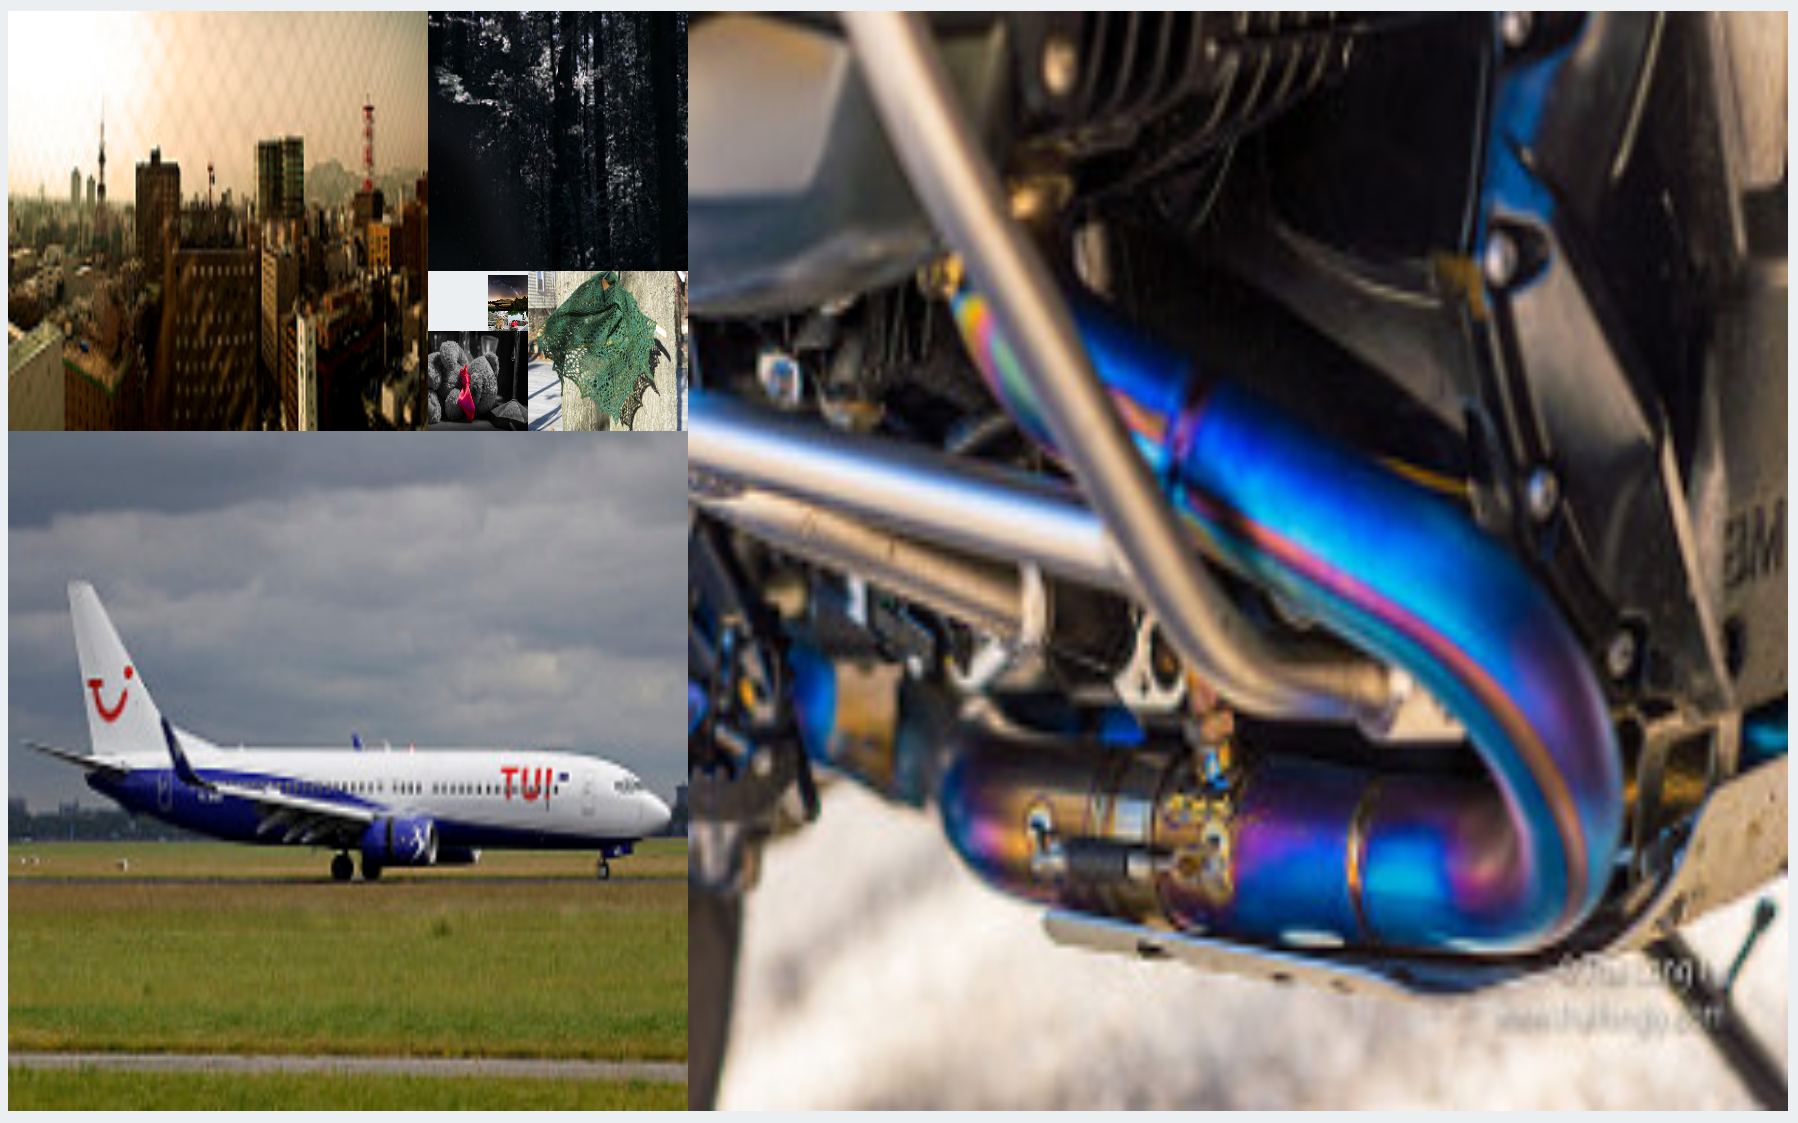
\includegraphics[width=\linewidth]{bluekittenflickr}
\caption[Image spiral `blue kitten'---Flickr]{Image spiral for query `blue kitten'---Flickr}
\label{fig:imgspiralflickr}
\end{figure}

\paragraph{Getty:}
\begin{quotation}
  \begin{description}
  \vspace{-1cm}
    \item[keyword\_ids] Return only images tagged with specific keyword(s). Specify using a comma-separated list of keyword Ids. If keyword Ids and phrase are both specified, only those images matching the query phrase which also contain the requested keyword(s) are returned.
    \item[phrase] Search images using a search phrase.
  \end{description}
  \sourceatright{\autocite{GettyAPI}}
\end{quotation}

Getty uses the \py{phrase} parameter to set the query. It only creates one pataphysicalised query term from the original query and calls for ten results based on that. This decision was based on the quota restrictions\marginnote{§~\ref{s:quota}} defined by Getty. Their limit is based on calls per second rather than calls per day or month. This means we cannot run ten calls for each user query as we did with FLickr. The query ``blue kitten'' gets turned into the word ``racy'' which then calls the \ac{API} to retrieve ten results (see figure~\ref{fig:imgspiralgetty}\marginnote{\faicon{picture-o}~\ref{fig:imgspiralgetty}}). The results mostly show racing cars from various angles although one oddball snuck in too: an office scene Getty has deemed to be `racy' (a guy in a suit checking out a lady's behind while she's leaning over a laptop).

\begin{figure}[!htbp]
\centering
  \includegraphics[width=\linewidth]{bluekittengetty}
\caption[Image spiral `blue kitten'---Getty]{Image spiral for query `blue kitten'---Getty}
\label{fig:imgspiralgetty}
\end{figure}

\paragraph{Bing:}
\begin{quotation}
  \begin{description}
  \vspace{-1cm}
    \item[query] The user's search query string. The query string cannot be empty. The query string may contain Bing Advanced Operators\footnote{For example `AND', `OR', `imagesize:', `NOT', or `phrase'}. For example, to limit images to a specific domain, use the site: operator. To help improve relevance and the results, you should always include the user's query string in an insights query (see insightsToken). This parameter is supported only by the Image API; do not specify this parameter when calling the Trending Images API.
  \end{description}
  \sourceatright{\autocite{BingAPI}\footnote{Microsoft will discontinue this version of the current \ac{API} in December 2016. The new version is documented on \url{https://www.microsoft.com/cognitive-services/en-us/bing-image-search-api}.}}
\end{quotation}

The Bing function uses the \py{query} parameter to set the query in the same way as Getty.

\paragraph{YouTube:}
\begin{quotation}
  \begin{description}
  \vspace{-1cm}
    \item[q] The q parameter specifies the query term to search for. Your request can also use the Boolean NOT (-) and OR (|) operators to exclude videos or to find videos that are associated with one of several search terms. For example, to search for videos matching either ``boating'' or ``sailing'', set the q parameter value to boating|sailing. Similarly, to search for videos matching either ``boating'' or ``sailing'' but not ``fishing'', set the q parameter value to boating|sailing -fishing. Note that the pipe character must be URL-escaped when it is sent in your API request. The URL-escaped value for the pipe character is \%7C.
  \end{description}
  \sourceatright{\autocite{YouTubeAPI}}
\end{quotation}

Youtube works in a similar way too. The \py{q} parameter is set to the pataphysicalised query term and one call retrieves ten results.

Something else to consider is perhaps that it is not entirely clear how the internal search for each \ac{API} works. This means that there's a possibility that they do their own query expansion\marginnote{§~\ref{s:qexpansion}} in the background to find more matches.


\subsubsection{Quota}
\label{s:quota}

Each \ac{API} has a different quota for their subscription packages. At this stage this is not a problem but if usage of \url{pata.physics.wtf} were to increase by a lot then these limitations would cause issues. At that point there are two options: (1) live with these limits or (2) get funding to upgrade the subscriptions to these services.

\begin{description}
  \item[Flickr] \num{3600} queries per hour are free \autocite{FlickrGuideAPI}.
  \item[Getty] \num{5} calls per second, unlimited calls per day \autocite{GettyOverviewAPI}.
  \item[Bing] \num{5000} transactions per month are free. A transaction is one request that returns one page of results \autocite{BingAzureAPI}.
  \item[YouTube] \num{50000000} units per day, \num{300000} units per \num{100} seconds per user, and \num{3000000} requests per \num{100} seconds are free. A call to the video search method counts as \num{100} units \autocite{YouTubeAPI}.
  \item[Microsoft Translator] \num{2000000} characters per month are free. Note the quota relates to single characters, not words \autocite{TranslatorAPI}.
\end{description}


\section{Science Fiction}

A more theoretical aspect of this analysis is concerned with what was already discussed to an extent in chapter~\ref{ch:interpretation} (specifically sections~\ref{ss:anthropomorphism}, \ref{s:programmer}, \ref{s:mimicry} and \ref{s:babying}), namely the parallel between artificial creativity and \acl{AI}. 


\subsection{Creativity, Intelligence and Ethics}

Computer creativity falls into the same overarching category as computer intelligence (\ac{AI}) and computer ethics.




Cohen is the author of AARON, perhaps the longest-lived and certainly the most creative artificial intelligence program in daily use. Cohen viewed AARON as his collaborator. At times during their decadeslong relationship AARON was quite autonomous, responsible for the composition, coloring and other aspects of a work; more recently, AARON served Cohen by making drawings that Cohen would develop into paintings. Cohen's death is the end of a lengthy partnership between an artist and an artificial intelligence.\autocite{Cohen2016}

Cohen had no patience for the ``is it art?'' question. He showed AARON's work in the world's galleries, museums and science centers -- the Tate, the Stedelijk, the San Francisco Museum of Art, Documenta, the Boston Computer Museum, the Ontario Science Center, and many others. His audiences might have been drawn in by curiosity and the novelty of computer-generated art, but they would soon ask, how can a machine make such marvelous pictures? How does it work? The very questions that Cohen asked himself throughout his career.\autocite{Cohen2016}


\todo{aaron stuff}
\url{http://collections.vam.ac.uk/name/cohen-harold/6433/}

\begin{quotation}
  \ldots we'll be seeing an increasing number of artists turning to robotic art of one sort or another in the next five or ten years. We're already seeing some. It's also a pretty safe bet that for the most part they'll be using off-the-shelf robots; that the ``art'' will be manifested in dreaming up contexts they were never intended for; and the culture's definitions of art will change accordingly.
  \sourceatright{\autocite{Cohen2007}}
\end{quotation}

\begin{quotation}
  Shouldn't it be possible, I wondered, to write the rules for generating material for a painting and then simply follow the rules?  In this way, it would be almost as if the painting was painting itself; and I would be relieved of the uncertain task of inventing on a day-to-day basis. 

  That was a little naïve, of course; it simply shifted the burden of invention to another place, another level. I'm still inventing on a day to day basis, but now it's likely to be algorithms for doing particular tasks that I'm inventing.
  \sourceatright{\autocite{Cohen2007}}
\end{quotation}

\begin{quotation}
  I'd like to end with a couple of observations about AARON's algorithm. Firstly; I think it's fair to say that nothing of what has happened could have happened unless I had drawn upon a lifetime of experience as a colorist.  I've evidently managed to pack all that experience into a few lines of code,  yet nothing in the code looks remotely like what I would have been doing as a painter, and AARON's algorithm isn't something a human artist could apply by hand, so to speak.
  \sourceatright{\autocite{Cohen2007}}
\end{quotation}

\begin{quotation}
  It's twenty years since I first realized that I could never turn AARON into a colorist by having it emulate my own expertise; in that case simply because it lacked the hardware upon which that expertise depended. Now I have AARON exercising an algorithm that couldn't be emulated by human colorists, presumably because they lack the hardware to do what AARON does. (and by hardware, in this case I mean the intellectual machinery that can build a stable enough representation and juggle enough variables, as AARON does in running the algorithm.) 
  \sourceatright{\autocite{Cohen2007}}
\end{quotation}

\begin{quotation}
  None of this would be interesting if AARON were an indifferent colorist. But I think I can claim, without undue immodesty, that AARON is a world-class colorist, significantly more inventive and infinitely more productive than I ever was myself. And I conclude that, after decades of expert systems  built to simulate human expertise, AARON has emerged as an expert in its own right. That marks a significant change of state, a change of level, in the never-ending pursuit of autonomy, not merely an incremental change in what the program is able to do. 
  \sourceatright{\autocite{Cohen2007}}
\end{quotation}

\begin{quotation}
  If I were writing AARON's biography today, I might almost say that AARON was a twinkle in its parent's eye in 1963; it was conceived in 1972 but not born until 2006. It has been a long gestation, and right now the parent is struggling to direct an unruly child, keeping it fed and changing its diapers. He has no idea when the child will be potty-trained, much less how long it will be before it reaches adulthood.
  \sourceatright{\autocite{Cohen2007}}
\end{quotation}




Where does this project stand in the wider world and the progress of computing, \ac{AI} and creativity? \ac{AI} and robotics is alluring as a research topic because it is so prevelant in Science Fiction. Computer creativity rarely plays a centrol role though. We can regularly read headlines that tell us that yet another kind of \ac{AI}-bot has won some game against a human player. Or we see videos of some innovative ground-breaking kind of new robot which claims to be near human-like (and yet cannot walk up stairs easily or hold a decent conversation). There are many examples of advances that are hailed as the next big thing which aren't all that great in the grand scheme of things. 

\subsection{AI}
This is also evident in games, for example \ac{VR} and \ac{AR}. The Oculus Rift and similar systems are advertised so much you might believe they are actually about to hit mainstream and every kid will own a \ac{VR} console and headset. Yet they are still way too expensive to be mainstream and motion sickness is also still an issue (and probably always will). These industries are so ``hip'' any publication is seen as the new cool thing without taking into account the history and work that has been done previously in perhaps slightly different disciplines. This is the case for example with a recent article on \ac{VR} sickness and how to compat it. This is a well known problem already---motion sickness already exists in normal games. Similar to epilepsy problems.

\todo{find links for motion sickness}
\todo{find links for epilepsy}
\todo{find links for oculus rift and pokenmon go etc}

\ac{AR} has very recently received a massive boom thanks to Pokenmon Go (released in Australia, New Zealand and the USA in July 2016). It has become a phenomenon since then.
\todo{find pokemon links}

What about IBM's Watson\footnote{See \url{http://www.ibm.com/watson/}}, Microsofts Twitter \ac{AI} chatbot Tay\footnote{See \url{https://web.archive.org/web/20160414074049/https://www.tay.ai/} for an archived version of the original website which is now offline. See also \url{https://twitter.com/tayandyou}, \url{https://www.theguardian.com/technology/2016/mar/24/tay-microsofts-ai-chatbot-gets-a-crash-course-in-racism-from-twitter}, and \url{https://www.theguardian.com/technology/2016/mar/30/microsoft-racist-sexist-chatbot-twitter-drugs}. Wikipedia also has a good article and sources on Tay: \url{https://en.wikipedia.org/wiki/Tay_(bot)}}, Google's AlphaGo\footnote{See \url{https://deepmind.com/alpha-go}} and Hanson Robotics Sophia robot\footnote{See \url{http://www.hansonrobotics.com/}}? How does this relate to my work? Practially of course they are all unrelated. On a deeper level though we can start asking interesting questions. 

https://www.engadget.com/2016/08/07/ibms-watson-ai-saved-a-woman-from-leukemia/
https://xkcd.com/1619/ XKCD WATSON

\begin{description}
  \item[IBM Watson] Watson is a question answering expert system. It famously won against human Jeopardy! champions in 2011.
  \item[Microsoft Tay] 
  \item[Google AlphaGo] AlphaGo is a system for playing the game Go. It won against a top human professional player in 2015.
  \item[Hansen Sophia]
\end{description}

I think these are interesting examples to study since they are supposedly on the forefront of \ac{AI} development. Life-like robots like Sophia still live in the `uncanny valley'. Her voice is creepy and unhuman, her intelligence or her capabilities if understanding conversations are clearly flawed (as shown by her viral remark about supporting genocide).\todo{check} Watson is clever and fast in finding answers for specific questions but he still had problems with humour (e.g. BLAHBLA\todo{find example}) but information lookup is arguably fairly easy and straightforward process within \ac{IR}---sure, it requires processing power and memory storage or access but it is based on simple matching of keywords, not any fancy heuristic algorithms. Microsofts twitter chatbot went viral and users `taught' it nasty swearwords \todo{check} quickly and Microsoft had to take the bot down. It has since apologised although any official documentation on it has disappeared \todo{check}. Google's AlphaGo has been hailed as a breakthrough in \ac{AI} but similar to Watson it is a very targeted and limited program. 

To me it seems the real breakthrough happens when (and if) the first robots appears which isn't as big as a house, can play Go, Chess and hide-and-seek, geniunely manages to get around he uncanny valley effect, has vast knowledge in his memory for instant information lookup, can hold a normal conversation without causing a war, etc, etc---you get the picture. General \ac{AI} is where it's at. Humans can do all the things we do. Children aren't born with only a single function. Imagine a world where humans only have one specialism and can;t do anything else. Mary is a Chess player but can't move her arms. Bob is a medical diagnosis expert but he can't hold a conversation. Movement, speech, memory---they are all vastly complex systems. And I haven't even touched creativity yet.

\todo{whats the point im making? how does this relate to my work?}
Perhpas this `uncanny valley' exists in creativity too. If a robot who looks vaguely human but not quite well enough, or he/she/it sounds almost human but not quite---perhaps if a robot can crack a joke like a human but not quite---perhaps this could be considered uncanny valley too? The philosphical zombies I mentioend in chapter~\ref{ch:interpretation}\marginnote{§~\ref{ch:interpretation}} live in this uncanny valley?

\todo{p and H creativity for computers?}


\subsection{Brains}

I'm not talking about the beer or the zombie food but rather research into the human brain (or animal brains) and attempts to model it on a computer. 

The motivation here is that once we understand how the brain works, perhaps we can understand how certain cognitive processes really work and this of course include creativity.

This is no easy task of course. Chris Chatham talks about ten ``important Differences Between Brains and Computers''\footnote{\url{http://scienceblogs.com/developingintelligence/2007/03/27/why-the-brain-is-not-like-a-co/}} which give a good overview of some of the dificulties of trying to model a brain as is. We can't just do a 1-1 copy.

\begin{quotation}
  \begin{enumerate}
    \item Brains are analogue; computers are digital
    \item The brain uses content-addressable memory
    \item The brain is a massively parallel machine computers are modular and serial
    \item Processing speed is not fixed in the brain; there is no system clock
    \item Short-term memory is not like RAM
    \item No hardware/software distinction can be made with respect to the brain or mind
    \item Synapses are far more complex than electrical logic gates
    \item Unlike computers, processing and memory are performed by the same components in the brain
    \item The brain is a self-organising system
    \item Brains have bodies
    \item	The brain is much, much bigger than any [current] computer
  \end{enumerate}
\sourceatright{Chris Chatham}
\end{quotation}

To bring this into perspective Ray Kurzweil claims the brain is capable of $10^{16}$ operations per second \citeyear[p.194]{Kurzweil2013}. Japan's K-computer (the worlds largest super computer as of 2016) currently has that power---10 petaflops. The ``Blue Brain Project'' is aiming to model $10^17$ bytes of memory and $10^{18}$ flops by 2023 \autocite[p.125]{Kurzweil2013}.
\todo{find k-computer reference}

There are currently some major research projects going on. One of them is the ``Human Brain Project'' \autocite{Walker2012}.

\begin{draft}
quotes:

Our brain consumes about 30W, the same as an electric light bulb, thousands of times less than a small supercomputer. \autocite[p.17]{Walker2012}

For environmental and business reasons, vendors have set themselves the goal of containing energy consumption to a maximum of 20 megawatts  \autocite[p.41]{Walker2012}

the 1 PFlop machine at the Jülich Supercomputing Centre could simulate up to 100 million neurons – roughly the number found in the mouse brain. \autocite[p.41]{Walker2012}

Cellular-level simulation of the 100 billion neurons of the human brain will require compute power at the exascale (1018 flops). \autocite[p.41-42]{Walker2012}

2017 petascale 50petabytes memory + 50 petaflops + <=4MW power

2021 exascale 200petabyte memory + 1exaflop

A second, equally important goal will be to prepare the procurement of the HBP Pre-exascale-supercomputer. By 2017/18, Jülich plans to procure a Big Data-centred system with at least 50 PBytes of hierarchical storage-class memory, a peak capability of at least 50 PFlop/s and a power consumption <= 4 MW. The memory and computational speed of the machine will be sufficient to simulate a realistic mouse brain and to develop first-draft models of the human brain. (The rest of the hardware roadmap targets an exascale machine in 2021/2022 with a capability of 1 EFlop/s and a hierarchical storage-class memory of 200 PB).\footnote{https://www.humanbrainproject.eu/high-performance-computing-platform}

\end{draft}

Why Minds Are Not Like Computers \autocite{Schulman2009}
Software – Hardware == Mind – Brain ??? analogy

"The power of the computer derives not from its ability to perform complex operations, but from its ability to perform many simple operations very quickly."

Layers of abstraction in computers:\\
1.	user interface\\
2.	high level programming language\\
3.	machine language\\
4.	proessor microarchitecture\\
5.	Boolean logic gates\\
6.	transistors\\

layers of abstraction in brain:\\
1.	personality?\\
2.	Thinking?\\
3.	Chemical /electrical signals/activity?\\
4.	Divided Brain regions/structure\\
5.	Neurons\\
6.	Dendrites (input) and axons (output)?\\


Computers are faster and better than humans in many tasks already.

\begin{quote}
"The weaknesses of the computational approach include its assumption that cognition can be reduced to mathematics and the difficulty of including noncognitive factors in creativity." \autocite[p.457]{Mayer1999}
\end{quote}

\todo{find references}
\todo{neural networks and other models based on the brain}

Perhaps we need to have that complete picture of how the brainw orks in order to understand human creativity. I would argue computer creativity is part of general \ac{AI}, and for general \ac{AI} we need massive amounts of general knoweldge.
\todo{common sense research}
\todo{again talk about how this is relevant for my project}
\paragraph{Expert Systems vs General AI}
Is computer creativity an expert system or does it fall into general \ac{AI}? 

\paragraph{Machines self-assessing}
Perhaps there is an argument that if humans are the only entities who can judge whether another human is being creative, then machines should be assessing themselves. This is a paradoxical concepts though. Since machines are products made my humans, they can never be autonomous in that sense. If machines had evolved like other animals besides us this argument might hold but obviously that is not the case.


\section{Design}

It is interesting to note how different the search results are perceived when presented in a different style (e.g. list rather than poem). This could be studied using questionnaires and interviews or eye tracking tools to find out what users prefer or perceive as more creative for example (see chapter~\ref{ch:aspirations},~\ref{ch:aspirations}). 

Figures~\ref{fig:poemtree},~\ref{fig:listsourcetree}~and~\ref{fig:listalgotree} show the three different text result styles. The poetry\marginnote{\faicon{picture-o}~\ref{fig:poemtree}} is compact and invites users to read all \num{14} (or less) lines. The two list styles\marginnote{\faicon{picture-o}~\ref{fig:listsourcetree}~\&~\ref{fig:listalgotree}} are much longer and involve a lot of scrolling to navigate, which might deter users from actually reading many of the results.

\begin{figure}[!htbp]
\centering
  \includegraphics[width=\linewidth]{poemtree}
\caption[Results as poem]{Results in poem form for query `tree'---Shakespeare}
\label{fig:poemtree}
\end{figure}

\begin{figure}[!htbp]
\centering
  \includegraphics[width=\linewidth]{listsourcetree}
\caption[Results as list by sources]{Results as list by sources for query `tree'---Shakespeare}
\label{fig:listsourcetree}
\end{figure}

\begin{figure}[!htbp]
\centering
  \includegraphics[width=\linewidth]{listalgotree}
\caption[Results as list by algorithm]{Results as list by algorithm for query `tree'---Shakespeare}
\label{fig:listalgotree}
\end{figure}


\section{Meta}

\subsection{Management}
\todo{add file for appendix with full git history}

On a different note, the project was completed over X years which includes an interruption and later on only a part time commitement.

I kept the project in a ``git repository''. Git is a version ontrol system that allows users to roll-back on changes and I further pushed my work to GitHub to make sure hardware failure or human error (i.e. lost or stolen property) would not affect my work. 

To understand git you need to know what commits are. They are the thing where I save my current state of the project and give it a description.

Below you can see a shortened version of the timeline of my commits between 20XX and the time of submission of this thesis. A full version can be found in appendix XYZ. You can see from this the time between programming work I did on \url{pata.physics.wtf} and its predecessors.

\todo{add calendar screenshot of github contributions}
\todo{links to git and github}

\begin{verbatim}
  *   10f61f9  Sun 08 May 2016	 (HEAD -> api, origin/api) Merge remote-tracking branch 'refs/remotes/origin/master' into api
  |\  
  * | 71437f6  Tue 18 Aug 2015	 Flickr and Bing work, radio buttons work
  * | 6c552aa  Wed 12 Aug 2015	 Fixed image problem but not video.
  | | * 1cbb63d  Tue 11 Aug 2015	 (origin/thesis) Update textsurfer.py
  | |/  
  |/|   
  * | 0ebff0d  Tue 11 Aug 2015	 Analytics enabled again
  * | 703f977  Tue 11 Aug 2015	 Problems solved.
  * | 74a1fae  Tue 11 Aug 2015	 About to change l\_dict to dict of dict
  * | 0935b23  Mon 10 Aug 2015	 BUG FUCKER
  * | 4f7d91e  Mon 10 Aug 2015	 Turn debug off
  * | 58f0c2b  Mon 10 Aug 2015	 Button styling done
  * | 59add58  Mon 10 Aug 2015	 Email problem solved
  * |   f1b2d40  Sun 09 Aug 2015	 Merge branch 'Deploy' into thesis
  |\ \  
  | * | 435cb2d  Sun 09 Aug 2015	 Deployment works, added analytics
  | * | 8a63dc7  Sat 08 Aug 2015	 gunicorn runs locally fine.
  | * | 2861407  Sat 08 Aug 2015	 Revert 5f2c957..4026965
  | * | 4026965  Sat 08 Aug 2015	 Tests
  * | |   8f2eeab  Sat 08 Aug 2015	 Merge branch 'w3' into thesis
  |\ \ \  
  | |/ /  
  | * | 5f2c957  Sat 08 Aug 2015	 Stuff
  | * | 873153c  Fri 07 Aug 2015	 Tiny cleanup
  | * | 05d5760  Thu 06 Aug 2015	 Random Poems and Emailing works
  | * | 657126c  Wed 05 Aug 2015	 Random poems work - without links though
  | * | 3d31ea9  Wed 05 Aug 2015	 Randomise still only works once, count ok
  | * | 5f1d45b  Wed 05 Aug 2015	 Randomise poem works ONCE
  | * | c583341  Wed 05 Aug 2015	 Poem subtabs, email poems done
  | * | f1b3878  Wed 05 Aug 2015	 Hiding divs
  | * | a6939c4  Tue 04 Aug 2015	 huh?
  | * | e6b411d  Tue 04 Aug 2015	 Poem emails WORK Fuck YEAH!
  | * | 4b6b170  Tue 04 Aug 2015	 Test email
  | * | 24e356c  Tue 04 Aug 2015	 Better load icon
  | * | e6ae736  Tue 04 Aug 2015	 loading icon version 1
  | * | 51b43e2  Tue 04 Aug 2015	 Added 4th pictures
  | * | f2d8a83  Mon 03 Aug 2015	 Minor fixes
  * | |   1ddb03d  Mon 03 Aug 2015	 Merge branch 'w3' into thesis
  |\ \ \  
  | |/ /  
  | * | ca4eab3  Mon 03 Aug 2015	 Pretty good state.
  | * | 9370334  Mon 03 Aug 2015	 working on list display of images
  | * | e1f1ead  Mon 03 Aug 2015	 Stylesheets sorted and cleaned files
  * | |   9732d5b  Mon 03 Aug 2015	 Merge branch 'w3' into thesis
  |\ \ \  
  | |/ /  
\end{verbatim}

\spirals

I also kept the thesis under git version control. Since the thesis was written in \LaTeX you could almost say I `programmed' it. Below is an outline of the commit history for this thesis.

\begin{verbatim}
* 3f06260	 Edited readme again
* c721b33	 Edited readme
* ffbdb4b	 Edited readme
* 8870b3d	 Added gitignore file
* ba1a9c2	 Second commit
* 244c4b3	 First commit
\end{verbatim}


\subsubsection{Development}

doing the analysis really helped revising and improving the code.



\subsection{Thesis}

\subsubsection{Part Spirals}

Each new thesis part contains a word spiral based on a poem generated by \url{pata.physics.wtf} using the a part of the title as keyword. They represent the pataphysical (Archimedean) spiral.

\begin{enumerate}
  \item Preface --- \emph{pre}
  \item Hello World --- \emph{hello}
  \item Tools of the Trade --- \emph{trade}
  \item The Core: Techno-Logic --- \emph{core}
  \item The Core: Techno-Practice --- \emph{practice}
  \item Meta-Logicalysis --- \emph{meta}
  \item Happily Ever After --- \emph{after}
  \item Postface --- \emph{post}
\end{enumerate}

\subsubsection{Chapter Poetry}

Each chapter opens with a poem generated by \url{pata.physics.wtf} using a part of the chapter title as keyword.

\begin{enumerate}
  \item Introduction --- \emph{intro}
  \item Inspirations --- \emph{inspiration}
  \item Methodology --- \emph{method}
  \item Pataphysics --- \emph{pata}
  \item Creativity --- \emph{creativity}
  \item Technology --- \emph{technology}
  \item Evaluation --- \emph{evaluation}
  \item Foundations --- \emph{foundation}
  \item Interpretation --- \emph{interpretation}
  \item Implementation --- \emph{implementation}
  \item Applications --- \emph{application}
  \item Patanalysis --- \emph{patanalysis}
  \item Aspirations --- \emph{aspirations}
  \item Observations --- \emph{observations}
\end{enumerate}

\todo{say more, check keywords, potentially generate new poems}





\section*{creative analysis}
\begin{draft}
  literary deconstruction and recombining to make new creative output? \\
  perception of results (poetry, source, algorithm) \\
  discuss applications from before (stimulates creative detour away from the obvious) \\

  How does this relate to Oulipo and Pataphysics? 

  Perhaps this is where I should talk a bit about the perception of results in their different output formats/styles. The poetry is automatically read with more gravity. Sorting by sources is a game of exploration or algorithms which becomes a game of finding the similarities within the result sets. They are different ways to view the same things and yet have a drastic influence of how the results are perceived. This also applies to the image and video search. Presenting results in spiral form is weird. Its hard to see where one image ends and another starts, they just kind of blur into each other. When listed as a list they immediately become more boring.

  talk abit about what the original plan was for some of the big changed elements in the website, e.g. the image search running 10 times on different keywords rather than running once with 10 results for the same keyword.
\end{draft}


DELETE EVERYTHING FROM BELOW HERE:


\begin{draft}
DELETE THIS

In this section we consider the possible uses and applications for the proposed creative search tool.

Our target audience is not quite as broad as that of a general search engine like Google. Instead, we aim to specifically cater for users who can appreciate creativity or users in need of creative inspiration. Users should generally be educated about the purpose of the search tool so that are not discouraged by what might appear to be nonsensical results. Users could include artists, writers or poets but equally anybody who is looking for out-of-the-box inspirations or simply a refreshingly different search engine to the standard.

The way we display and label results produced by the tool can influence how the user perceives them. The current prototype for example separates the results into its three components but we could have equally just mixed them all together. The less transparent the processes in the background (e.g.\ which algorithm was used, how does the result relate to the query precisely, etc.) are for the user, the more difficult it might be to appreciate the search.

There are many ways a pataphysical search tool could be used across disciplines.

In literature, for example, it could be used to write or generate poetry, either practically or as a simple aid for inspiration. We are not limited to poetry either; novels, librettos or plays could benefit from such pataphysicalised inspirations. One can imagine tools using this technology that let you explore books in a different ordering of sentences (a sort of pataphysical journey of paragraph hopping), tools that re-write poems or mix and match them together. Even our simple prototype shows potential in this area and could be even more powerful if we extended it to include more base texts, for example the whole set of books contained in Faustroll’s library ([20] and also [12]). A richer body of texts (by different authors) would produce a larger index which would possibly find many more matches through WordNet and end in a more varied list of results.

From a computer science perspective it could be used as one of the many algorithms used by traditional search engines for purposes like query feedback or expansion (e.g. “did you mean … “or “you might also be interested in … “). Depending on how creative we want the search engine to be, the higher we would rank the importance of this particular algorithm. One of the concepts related to the search tool, namely patadata, could have an impact on the development of the Semantic Web. Just as the Semantic Web is about organizing information semantically through objective metadata, patadata could be used to organize information pataphysically in a subjective way.

The prototype tool is already being used in the creation of an online opera, provisionally entitled from [place] to [place], created in collaboration with The Opera Group, an award-winning, nationally and internationally renowned opera company, specialising in commissioning and producing new operas. In particular, it is being used to create the libretto for one of the virtual islands whose navigation provides the central storyline for the opera. The opera will premiere in 2013, and will continue to develop thereafter, deploying new versions of the tool as they appear.
\end{draft}






\stopcontents[chapters]

% !TEX root = ../main.tex

\chapter{Aspirations}
\label{ch:future}

\startcontents[chapters]

Mid the silence that pants for breath, \\
when I thought myself at my last gasp, \\
haine ou de l'ambition et qui se, \\
the pale motor vessel withdrew its blue breath toward the island's horizon.

As pure and simple as a powder puff, \\
such also was the ambition of others upon the like occasion, \\
there was hardly a breath of air stirring, \\
mon ancien cœur en une aspiration vers la vertu.

After drawing a long breath, \\
the silver ring she pull'd, \\
the suitor cried, or force shall drag thee hence.

For wild ambition wings their bold desire, \\
and with thine agony sobbed out my breath, \\
I will pull down my barns.

\minicontents

PROBLEMS ENCOUNTERED AND SUGGESTED SOLUTIONS

SHORTCOMINGS AND MISSING FUNCTIONALITY

\begin{itemize}
  \item Research in science and art
  \item Review paper? Pataphysics and creativity?
  \item Quantitative research questions
  \item Working definition for Pataphysics
  \item Examples for Pataphysics concepts
  \item Examples for types of creativity
  \item Examples for creative process
  \item Explain Leary's tables
  \item How can we use creative concepts discussed?
\end{itemize}


\section{Code}

FURTHER DEBUGGING OF CODE (IF NECESSARY)

\section{Interface}

DESIGN ASPECTS

IMPROVEMENTS / ALTERNATIVES TO USER INTERFACE DESIGN

\section{Algorithms}

IMPROVEMENTS / ALTERNATIVES TO ALGORITHMS

\section{Architecture}

IMPROVEMENTS / ALTERNATIVES TO ARCHITECTURE

\section{Research}

USER FEEDBACK (IF NECESSARY)

\stopcontents[chapters]


\phantomsection
% \addtocontents{toc}{\protect\vspace{20pt}}
\addcontentsline{toc}{part}{\texorpdfstring{HAPPILY EVER AFTER}{Conclusion}}
\partimage[width=\textwidth]{spiral_after.pdf}
\part{\texorpdfstring{H\scalebox{2.2}{$\boldsymbol\forall$}PPILY \scalebox{2.2}{$\boldsymbol\Sigma$}V\scalebox{2.2}{$\boldsymbol\Sigma$}R \scalebox{2.2}{$\boldsymbol\forall$}FT\scalebox{2.2}{$\boldsymbol\Sigma$}R}{Conclusion}}
\label{p:outro}
% !TEX root = ../main.tex

\chapter{Observations}
\label{ch:observations}

\startcontents[chapters]

\vfill

Paying no attention to his fellow mites, \\
mérite pas que vous fassiez attention à moi, \\
and told him to look after a calf she had bought, \\
and whilst he was looking at it attentively.

Phedon the fact affirm'd, \\
comment peux, \\
ne faites aucune attention à mon air, \\
in fact.

For sure Ulysses in your look appears, \\
was nearly out of her mind, \\
I omitted none of the common forms attending a royal audience.

And the consequences attending thereupon, \\
impotent of mind, \\
shape at the moment of looking at the time.

\newpage
\minicontents
\spirals

\todo{summarise thesis, contributions etc. conclude by comparing against introduction}


\section{Summary}

I've done blah blah blah.


\section{Contributions}

mention to whom these could be useful


\section{Conclusion}

thanks for reading


\stopcontents[chapters]


% BACK
\appendix

\phantomsection
% \addcontentsline{toc}{chapter}{References}
% \bibliography{back/bib} % NATBIB
% the following two lines are needed so that Bibliography 
% is promoted to root level of pdf hierarchy
% and not part of the previous part as a "chapter"
\bookmarksetup{startatroot}
\addtocontents{toc}{\bigskip}
\printbibliography % BIBLATEX
\clearpage

% \phantomsection
% \addtocontents{toc}{\protect\vspace{20pt}}
% \addcontentsline{toc}{chapter}{INTERLUDE}
% \addtocontents{toc}{\protect\vspace{10pt}}
\pagestyle{empty}

\chapter*{INTERLUDE III}
\label{interlude3}

% analysis
% aspirations
% observations





\clearpage

\phantomsection
% \addtocontents{toc}{\protect\vspace{20pt}}
\addcontentsline{toc}{part}{\texorpdfstring{POSTFACE}{Appendix}}
\partimage[width=\textwidth]{spiral_post.pdf}
\part{\texorpdfstring{POST\scalebox{2.5}{\frownie{}}}{Appendix}}
% !TEX root = ../main.tex

\chapter{Random}
\label{app:random}


\section{Random Sentences}
\label{s:appsentences}

\begin{minted}{haskell}
in posthumous collaboration
the decomposing brain goes on working after death and it is its dreams that are Paradise
plagiarism by anticipation
the applause of silence is the only kind that counts
to understand pataphysics is to fail to understand pataphysics
duration is the transformation of a succession into a reversion
god is the tangential point between zero and infinity
laughter is born out of the discovery of the contradictory
ha ha
the aesthetic of formal constraint
the unique imaginary solution to the absence of problems
the contemporary relationship between science and poetry
a huge and elaborately constructed hoax
only those who attempt the absurd achieve the impossible
the random is opposed to the deterministic
pure multiplicity irreducible to any other sort of unity
persistence and perseverance to buttress a fleeting existence
enfolding a subject laterally, associatively
a doctrine of correspondences, counterpoised by the exotic charm of another system of thought
double negative is necessary to stop the mind believing
the absence of contradictory evidence is not proof of a theory's validity
very wrong in very important ways
no one point of view is final
unification of opposites
an athletic aesthetics of intuitive and instantaneous judgements
constantly diverted from any objective by the very progress which their energy sustains
imagination envisions the reconciliation of the individual with the whole
behind the illusion lies knowledge
a biomolecular bibliomecha of breathtaking beauty
indubitably coherent yet absolutely nonsensical
stylistic and formal experimentation can not be dismissed as purely apolitical
variable phoneme sequences in suspension within a cloud of relative epi-cultural etymologies
speculative solutions for imaginary problems
nonsense is nonsense only when we have not yet found the point of view from which it makes sense
laughter is the discord between tensions being resolved
read with intention to rewrite
a fractal geometry of momentums
minimizing energy, crystallizing latent structure, pleasure is understood as a practice, and accumulates as experience
don't fall out of love
the `something like', the pseudo
the text transforms itself as soon as it is understood
adaptation of archaic mental structures to new environments
a beautifully controlled yet hideously wasteful catastrophe
driven by compulsive urgency to constantly reconceive the whole idea
writing the unrightable wrongs
prisoners of conscience
machina sapiens negotiating the transformation of what is mortal into what is immortal
database hyper-archive applications stimulating relaxation
smelling of the rain it falls on the way down
a thousand ways to greet the dawn
how far up the chain can you put this without ambiguity
a gentle kitten is licking the inside of my heart
was this constrained by you, or restrained by the concept
adjoining always antiquated permutation
joint ventures can go too far away
nowhere to be found here and elsewhere
engender links to a balancing veneration
coerce to do as a sizeable unprocessed primer
plain up be a best concoction in the words
the farcical pandemonium of technology
it is not true that there were any nails
this discovery opens the door into a completely new anti-world
extending as far beyond metaphysics as the latter extends beyond physics
turn the world upside down and inside out
the law of the ascension of a vacuum toward a periphery
the anti-world God not only plays dice, he spells his name backwards
in the absence of a butler, where does the gun fit in
space is defined by simultaneity
time is a flowing stream, a liquid in uniform rectilinear motion
space is a solid, a rigid system of phenomena
the deceleration of our habitual duration conserved by inertia
a perfect elastic solid
movement into the past consists in the perception of the reversibility of phenomena
relativity is absolute
all observations depend on viewpoint and the scale of the scientist
the clinamen, subjective viewpoint and anthopocentrism all rolled into one
the identity of opposites
making negatives do the work of positives
in this year eighteen hundred and ninety-eight
the twenty-seven equivalents
the virgin, the bright, and the beautiful today
the fifth letter of the first word of the first act
voices asymptotic towards death
an epiphenomenon is that which is superinduced upon a phenomenon
concerning the amorphous isle
like soft coral, amoeboid and protoplasmic
searching desperately under the quinuncial trees for the venerable absent one
the night computed its hours
a remarkable epizootic disease
the eternal nothingness
love looks exactly like an iridescent veil and assumes the masked face of a chrysalis
in a telepathic letter
homo est deus
$\infty$ -0 -a + a + 0 = $\infty$
with the aim of computing the qualities of the French
the inferno of subjectivity
\end{minted}


\section{Heisenberg Quote}
\label{s:heisenberg}

\begin{quotation}
  The overly forceful insistence on the difference between scientific and artistic cognition quite likely derives from the incorrect notion that concepts are firmly attached to `real objects', as if words had a completely clear and definite meaning in their relationship to reality and as if an accurate sentence, constructed from those words, could deliver an intended `objective' factual situation to a more or less absolute degree. But we know, after all, that language too only grasps and shapes reality by turning it into ideas, by idealizing it. Language, too, approaches reality with specific mental forms about which we do not know right away which part of reality they can comprehend and shape. The question about `right' or `wrong' may indeed be rigorously posed and settled within an idealization, but not in relation to reality. That is why the last measure available for scientific knowledge as well is only the degree to which that knowledge is able to illuminate reality or, better, how that illumination allows us `to find our way' better. And who could question that the spiritual content of a work of art too illumines reality for us and makes it translucent? One must come to terms with the fact that only through the process of cognition itself can we determine what we are to understand by `cognition'. That is why any genuine philosophy, too, stands on the threshold between science and poetry. \sourceatright{\autocite{Heisenberg1942}}
\end{quotation}


\section{Digital Humanities Methodology Field Map}
\label{s:dhmap}

The full \textit{Field map of digital humanities: emerging methods and genres} by Burdick et al. \citeyear{Burdick2012}.

\begin{multicols}{2}\raggedright
\begin{itemize}
  \item enhanced critical curation
  \begin{itemize}
    \item digital collections
    \item multimedia critical editions
    \item object-based argumentation
    \item expanded publication
    \item experiential and spatial
    \item mixed physical and digital
  \end{itemize}
  \item augmented editions and fluid textuality
  \begin{itemize}
    \item structured mark-up
    \item	natural language processing
    \item	relational rhetoric
    \item	textual analysis
    \item	variants and versions
    \item	mutability
  \end{itemize}
  \item scale: the law of large numbers
  \begin{itemize}
    \item quantitative analysis
    \item	text-mining
    \item	machine reading
    \item	digital cultural record
    \item	algorithmic analysis
  \end{itemize}
  \item distant/close, macro/micro, surface/depth
  \begin{itemize}
    \item large-scale patterns
    \item	fine-grained analysis
    \item	close reading
    \item	distant reading
    \item	differential geographies
  \end{itemize}
  \item cultural analytics, aggregation, and data-mining
  \begin{itemize}
    \item parametrics
    \item	cultural mash-ups
    \item	computational processing
    \item	composite analysis
    \item	algorithm design
  \end{itemize}
  \item visualization and data design
  \begin{itemize}
    \item data visualization
    \item	mapping
    \item	information design
    \item	simulation environments
    \item	spatial argument
    \item	modelling knowledge
    \item	visual interpretation
  \end{itemize}
  \item locative investigation and thick mapping
  \begin{itemize}
    \item spatial humanities
    \item	digital cultural mapping
    \item	interconnected sites
    \item	experimental navigation
    \item	geographic information systems (GIS)
    \item	stacked data
  \end{itemize}
  \item the animated archive
  \begin{itemize}
    \item user communities
    \item	permeable walls
    \item	active engagement
    \item	bottom-up curation
    \item	multiplied access
    \item	participatory content creation
  \end{itemize}
  \item distributed knowledge production and performative access
  \begin{itemize}
    \item global networks
    \item	ambient data
    \item	collaborative authorship
    \item	interdisciplinary teams
    \item	use as performance
    \item	crowd-sourcing
  \end{itemize}
  \item humanities gaming
  \begin{itemize}
    \item user engagement
    \item	rule-based play
    \item	rich interaction
    \item	virtual learning environments
    \item	immersion and simulation
    \item	narrative complexity
  \end{itemize}
  \item code, software, and platform studies
  \begin{itemize}
    \item narrative structures
    \item	code as text
    \item	computational processes
    \item	software in a cultural context
    \item	encoding practices
  \end{itemize}
  \item database documentaries
  \begin{itemize}
    \item variable experience
    \item	user-activated
    \item	multimedia prose
    \item	modular and combinatoric
    \item	multilinear
  \end{itemize}
  \item repurposable content and remix culture
  \begin{itemize}
    \item participatory Web
    \item	read/write/rewrite
    \item	platform migration
    \item	sampling and collage
    \item	meta-medium
    \item	inter-textuality
  \end{itemize}
  \item pervasive infrastructure
  \begin{itemize}
    \item extensible frameworks
    \item	heterogeneous data streams
    \item	polymorphous browsing
    \item	cloud computing
  \end{itemize}
  \item ubiquitous scholarship
  \begin{itemize}
    \item augmented reality
    \item	web of things
    \item	pervasive surveillance and tracking
    \item	ubiquitous computing
    \item	deterritorialization of humanistic practice
  \end{itemize}
\end{itemize}
\end{multicols}

\section{Penn Treebank}
\label{s:penntreebank}

\begin{multicols}{2}\raggedright
\begin{description}[leftmargin=1.5cm]
  \item[CC   ] Coordinating conjunction              
  \item[CD   ] Cardinal number                       
  \item[DT   ] Determiner                            
  \item[EX   ] Existential \textit{there}            
  \item[FW   ] Foreign word                          
  \item[IN   ] Preposition/subordinating conjunction 
  \item[JJ   ] Adjective                             
  \item[JJR  ] Adjective, comparative                
  \item[JJS  ] Adjective, superlative                
  \item[LS   ] List item marker                      
  \item[MD   ] Modal                                 
  \item[NN   ] Noun, singular or mass                
  \item[NNS  ] Noun, plural                          
  \item[NNP  ] Proper noun, singular                 
  \item[NNPS ] Proper noun, plural                   
  \item[PDT  ] Predeterminer                         
  \item[POS  ] Possessive ending                     
  \item[PRP  ] Personal pronoun                      
  \item[PP\$ ] Possessive pronoun                    
  \item[RB   ] Adverb                                
  \item[RBR  ] Adverb, comparative                   
  \item[RBS  ] Adverb, superlative                   
  \item[RP   ] Particle                              
  \item[SYM  ] Symbol (mathematical or scientific)   
  \item[TO   ] \textit\{to\}                         
  \item[UH   ] Interjection                          
  \item[VB   ] Verb, base form                       
  \item[VBD  ] Verb, past tense                      
  \item[VBG  ] Verb, gerund/present particle         
  \item[VBN  ] Verb, past particle                   
  \item[VBP  ] Verb, non-3rd ps. sing. present       
  \item[VBZ  ] Verb, 3rd ps. sing. present           
  \item[WDT  ] \textit{wh}-determiner                
  \item[WP   ] \textit{wh}-pronoun                   
  \item[WP\$ ] Possessive \textit{wh}-pronoun        
  \item[WRB  ] \textit{wh}-adverb                    
  \item[\#   ] Pound sign                            
  \item[\$   ] Dollar sign                           
  \item[.    ] Sentence-final punctuation            
  \item[,    ] Comma                                 
  \item[:    ] Colon, semi-colon                     
  \item[(    ] Left bracket character                
  \item[)    ] Right bracket character               
  \item["    ] Straight double quote                 
  \item[`   ] Left open single quote               
  \item[`` ] Left open double quote              
  \item['   ] Right close single quote             
  \item['' ] Right close double quote      
\end{description}      
\end{multicols}


\section{Thinking computers}
\label{s:think}

\begin{quotation}
  \begin{enumerate}
    \item \textbf{Can computers think?}
      \begin{itemize}
        \item Can computers have free will?
        \item Can computers have emotions?
        \item Can computers be creative?
        \item Can computers understand arithmetic?
        \item Can computers draw analogies?
        \item Can computers be persons?
        \item Is the brain a computer?
        \item Can computers reason scientifically?
        \item Are computers inherently disabled?
        \item Should we pretend that computers will never be able to think?
        \item Does God prohibit computers from thinking?
      \end{itemize}
    \item \textbf{Can the Turing test determine whether computers can think?}
      \begin{itemize}
        \item Is failing the test decisive?
        \item Is passing the test decisive?
        \item If a simulated intelligence passes, is it intelligent?
        \item Have any machines passed the test?
        \item Is the test, behaviouraly or operationally construed, a legitimate intelligence test?
        \item Is the test, as a source of inductive evidence, a legitimate intelligence test?
        \item Is the neo-Turing test a legitimate intelligence test?
        \item Does the imitation game determine whether a computer can think?
        \item Can the Loebner Prize stimulate the study of intelligence?
        \item Other Turing test arguments
      \end{itemize}
    \item \textbf{Can physical symbol systems think?}
      \begin{itemize}
        \item Does thinking require a body?
        \item Is the relation between hardware and software similar to that between human brains and minds?
        \item Can physical symbol systems learn as humans do?
        \item Can the elements of thinking be represented in discrete symbolic form?
        \item Can symbolic representations account for human thinking?
        \item Does the situated action paradigm show that computers can't think?
        \item Can physical symbol systems think dialectically?
        \item Can a symbolic knowledge base represent human understanding?
        \item Do humans use rules as physical symbol systems do?
        \item Does mental processing rely on heuristic search?
        \item Do physical symbol systems play chess as humans do?
        \item Other physical system arguments
      \end{itemize}
    \item \textbf{Can Chinese Rooms think?}
      \begin{itemize}
        \item Do humans, unlike computers, have intrinsic intentionality?
        \item Is biological naturalism valid?
        \item Can computers cross the syntax-semantics barrier?
        \item Can learning machines cross the syntax-semantics barrier?
        \item Can brain simulators think?
        \item Can robots think?
        \item Can a combination robot/brain simulator think?
        \item Can the Chinese Room, considered as a total system, think?
        \item Do Chinese Rooms instantiate programs?
        \item Can an internalized Chinese Room think?
        \item Can translations occur between the internalized Chinese Room and the internalizing English speaker?
        \item Can computers have the right causal powers?
        \item Is strong AI a valid category?
        \item Other Chinese Room arguments
      \end{itemize}
    \item \textbf{Can connectionist networks think?}
      \begin{itemize}
        \item Are connectionist networks like human neural networks?
        \item Do connectionist networks follow rules?
        \item Are connectionist networks vulnerable to the arguments against physical symbol systems?
        \item Does the subsymbolic paradigm offer a valid account of connectionism?
        \item Can connectionist networks exhibit systematicity?
        \item Other connectionist arguments
      \end{itemize}
    \item \textbf{Can computers think in images?}
      \begin{itemize}
        \item Can images be realistically be represented in computer arrays?
        \item Can computers represent the analog properties of images?
        \item Can computers recognize Gestalts?
        \item Are images less fundamental than propositions?
        \item Is image psychology a valid approach to mental processing?
        \item Are images quasi-pictorial representations?
        \item Other imagery arguments
      \end{itemize}
    \item \textbf{Do computers have to be conscious to think?}
      \begin{itemize}
        \item Can computers be conscious?
        \item Is consciousness necessary for thought?
        \item Is the consciousness requirement solipsistic?
        \item Can higher-order representations produce consciousness?
        \item Can functional states generate consciousness?
        \item Does physicalism show that computers can be conscious?
        \item Does the connection principle show that consciousness is necessary for thought?
      \end{itemize}
    \item \textbf{Are thinking computers mathematically possible?}
      \begin{itemize}
        \item Is mechanistic philosophy valid?
        \item Does G{\"o}del's theorem show that machines can't think?
        \item Does G{\"o}del's theorem show that machines can't be conscious?
        \item Do mathematical theorems like G{\"o}del's show that computers are intrinsically limited?
        \item Does G{\"o}del's theorem show that mathematical insight is non-algorithmic?
        \item Can automata think?
        \item Is the Lucas argument dialectical?
        \item Can improved machines beat the Lucas argument?
        \item Is the use of consistency in the Lucas argument problematic?
        \item Other Lucas arguments
      \end{itemize}
  \end{enumerate}
  \sourceatright{\autocite{Horn2009}}
\end{quotation}


\section{Oulipo}
\label{s:appoulipo}

\begin{multicols}{3}\raggedright
\begin{itemize}
  \item x mistakes y for z
  \item word ladder
  \item univocalism
  \item transplant
  \item threnodials
  \item tautogram
  \item spoonerism
  \item sonnet
  \item snowball
  \item sestina
  \item septina
  \item rhopalic verse
  \item quenina
  \item pumectation
  \item prisoner's restriction
  \item precooked language
  \item perverse
  \item perverb
  \item permutation
  \item paronomasia
  \item pangram
  \item palindrome
  \item oligogrammatic poem
  \item n + 7
  \item multiple sonnet
  \item multiple-choice narrative
  \item melting snowball
  \item measures
  \item mathews's algorithm
  \item machines for writing
  \item liponymy
  \item lipolexe
  \item lipogram
  \item lescurean permutations
  \item left-handed lipogram
  \item larding
  \item isopangram
  \item isomorphism
  \item isogram
  \item irrational sonnet
  \item inventory
  \item intersective novel
  \item inclusion
  \item imparmigianisation
  \item homovocalism
  \item homosyntactical translation
  \item homosemantic translation
  \item homophony
  \item homophonic translation
  \item homomorphism
  \item homolexical translation
  \item homoconsonantism
  \item holorhyme
  \item heterosexual rhyme
  \item heterogram
  \item haikuisation
  \item grammatical translation
  \item graeco-latin bi-square
  \item franglais
  \item eye-rhyme
  \item equivoque
  \item epithalamium
  \item eodermdrome
  \item end-to-end
  \item elementary morality
  \item eclipse
  \item deunglitsch
  \item delmas's method
  \item definitional literature
  \item cylinder
  \item constraint
  \item combinatorial literature
  \item clinamen
  \item chronogram
  \item chimera
  \item cento
  \item canada dry
  \item braised rhyme
  \item boolean poetry
  \item beautiful outlaw
  \item beautiful in-law
  \item bananagram
  \item axiomatic writing
  \item avalanche
  \item assonance
  \item asphyxiation
  \item arborescent text
  \item aphorism
  \item antonymy
  \item anterhymes
  \item analogue lexicon
  \item anagram
  \item algol poetry
  \item alexandrine
  \item acrostic
  \item acronymic poetry
\end{itemize}
\end{multicols}

% !TEX root = ../main.tex

% \chapter{Appendix A}
\chapter{Code}
\label{app:code}
% \lhead{Appendix A. \emph{Code}}

\section{Clinamen}

\begin{lstlisting}
def clinamen(word, i):
    out = set()
    items = [item for item in froll_dict if dameraulevenshtein(word, item) <= i]
    for item in items:
        if item != word:
            out.add(item)
    return out
\end{lstlisting}


\section{Damerau Levenshtein}

\lstinputlisting[language=Python,
                firstline=192, lastline=208]
                {back/textsurfer.py}

% !TEX root = ../main.tex

\chapter{WordNet}
\label{app:wordnet}

% !TEX root = ../main.tex

\chapter{Git History}
\label{app:git}


\section{Website Repository}

\begin{minted}{haskell}
* 0fbbfcd  |  Sat 15 Oct 2016  (HEAD -> master, origin/master, origin/HEAD) |  Deleted local log
* 504bcfa  |  Sat 15 Oct 2016  |  Added meta description
* a7e4a5d  |  Sun 02 Oct 2016  |  Updated about
*   64b0c9a  |  Sun 02 Oct 2016  |  Work in progress
|\  
| | *   76e1dbb  |  Fri 12 Aug 2016  (origin/live, live) |  Merge pull request #15 from Fania/master
| | |\  
| | |/  
| |/|   
| * |   5fd81f9  |  Fri 12 Aug 2016  (tag: v.4.1) |  Merge pull request #14 from Fania/thesis
| |\ \  
| | * | 331ddfe  |  Fri 12 Aug 2016  (origin/thesis) |  Comment out prints
| | * | 878cade  |  Fri 12 Aug 2016  |  Log updates
| | * | d894400  |  Fri 12 Aug 2016  |  Fixed results-reverbs-origins numbers
| | * | 7a64760  |  Fri 12 Aug 2016  |  Fixed holonyms and meronyms
| |/ /  
| * |   8efc58a  |  Fri 12 Aug 2016  |  Merge pull request #13 from Fania/live
| |\ \  
| | |/  
* | | c4b9eea  |  Thu 11 Aug 2016  |  About section update
|/ /  
| * 0f6353a  |  Thu 11 Aug 2016  (tag: v.4.0) |  Added new paper to about section
| * 0fd2af4  |  Thu 11 Aug 2016  |  Cleaned files
| *   1bf06c8  |  Thu 11 Aug 2016  |  Merge branch 'live' of https://github.com/Fania/pata.physics.wtf into live
| |\  
| * | 0b66aaf  |  Thu 11 Aug 2016  |  Enabled image and video in menu
| | *   15bdb1e  |  Thu 11 Aug 2016  |  Merge pull request #12 from Fania/master
| | |\  
| |/ /  
| | /   
| |/    
|/|     
* |   23ea5c6  |  Thu 11 Aug 2016  |  Merge commit
|\ \  
| |/  
* | 8f5708d  |  Thu 11 Aug 2016  |  Changed date
* |   3b32674  |  Thu 11 Aug 2016  |  Merge pull request #11 from Fania/dev
|\ \  
| * \   d480bfa  |  Thu 11 Aug 2016  (dev) |  Merge pull request #9 from Fania/prints
| |\ \  
| | * | 4adf2a2  |  Thu 11 Aug 2016  (prints) |  Added meronyms, got rid of prints again
| | * | b454247  |  Thu 04 Aug 2016  |  ppsent
| | * | dbb33cd  |  Thu 04 Aug 2016  |  ppsent fix
| | * | ef33367  |  Sat 23 Jul 2016  |  stuff
| | * | 6edc4a3  |  Tue 19 Jul 2016  |  ppsent prints
| | * | 3fa7ab6  |  Tue 19 Jul 2016  |  about to change ppsent
| |/ /  
| * | 96a7f8f  |  Mon 18 Jul 2016  |  log changes
| * | abdc8a1  |  Wed 06 Jul 2016  |  Revert "failed getty (3callspersec)"
| * | 975edb6  |  Wed 06 Jul 2016  |  failed getty (3callspersec)
| * | c9b6b82  |  Wed 06 Jul 2016  |  Prepping for rewriting Getty and Bing to run 10 times
| * | 62ad371  |  Wed 06 Jul 2016  |  Made Flickr Img List Vessel function standalone
| * | 8eaa132  |  Wed 06 Jul 2016  |  Fixed log printouts
| * | e6c1d5f  |  Tue 05 Jul 2016  |  flickr working with 10 images
| * | 916faa4  |  Tue 05 Jul 2016  |  10 images working
| * | 46b4209  |  Tue 05 Jul 2016  |  partially working imagelistvessel ith 10 results
| * | efe1893  |  Tue 05 Jul 2016  |  still fucking in progress
| * | f549bab  |  Sun 03 Jul 2016  |  work in progress
| * | f4fdbea  |  Sun 03 Jul 2016  |  trap for empty data items in js
| * | 178b63a  |  Sun 03 Jul 2016  |  half assed img search 10 results done
| * | b00fd7e  |  Sun 03 Jul 2016  |  Video working
| * | c99e8eb  |  Sun 03 Jul 2016  |  Getty works too.
| * | aeb081d  |  Sat 02 Jul 2016  |  Getty API down, flickr and Bing work
| * | d228062  |  Sat 02 Jul 2016  |  Flickr and Bing work
| * | c53b060  |  Sat 02 Jul 2016  |  Query is now 1 random item from pata set
| * | ac86e07  |  Sat 02 Jul 2016  |  Image search works again somehow
| * | 0c7713b  |  Tue 07 Jun 2016  |  work in progress
| * | 4fed23c  |  Tue 07 Jun 2016  |  added log with date and time
| * | 52c4394  |  Tue 07 Jun 2016  |  datetime log
|/ /  
| * 2dfa9d3  |  Mon 06 Jun 2016  (tag: v.3.5) |  Ready to deploy
| * 0cc8be1  |  Mon 06 Jun 2016  |  Added log
|/  
* 2c51dbc  |  Mon 06 Jun 2016  |  dot creeped into code
*   e49efa5  |  Mon 06 Jun 2016  |  pre-merge commit
|\  
* | 6c43cea  |  Mon 06 Jun 2016  |  pre-merge commit again
* |   af51ef4  |  Mon 06 Jun 2016  |  pre-merge commit
|\ \  
* \ \   4859e65  |  Mon 06 Jun 2016  |  pre merge commit
|\ \ \  
* | | | 26a1d9c  |  Mon 06 Jun 2016  |  test commit
| | | * 3ef1630  |  Mon 06 Jun 2016  |  readme updates
| | | * 06b070a  |  Mon 16 May 2016  |  git log stuff
| | | *   10f61f9  |  Sun 08 May 2016  |  Merge remote-tracking branch 'refs/remotes/origin/master' into api
| | | |\  
| |_|_|/  
|/| | |   
* | | | aa58f79  |  Sat 09 Apr 2016  |  screenshot
* | | | bea5474  |  Sat 09 Apr 2016  |  added screenshot
* | | | 7072f33  |  Sat 09 Apr 2016  (tag: v2.0) |  gitignore
| | | * 0e53ee6  |  Sat 09 Apr 2016  |  Working on new server stuff
| | | * a082595  |  Tue 05 Apr 2016  |  Update to Todo file
| | | * 6fbbd49  |  Sun 20 Mar 2016  |  pataphysicalisation work in progress
| | | * 80412e1  |  Sun 20 Mar 2016  |  Flickr, Getty and Bing working!
| | | * 00fd2c5  |  Sun 20 Mar 2016  |  radio buttons update properly
| | | * 7e03f4b  |  Wed 16 Mar 2016  |  Flickr OK Getty OK
| | | * df847d9  |  Wed 16 Mar 2016  |  Revert "Test revert commit"
| | | * 630bf1a  |  Wed 16 Mar 2016  |  Test revert commit
| | | * 62dfc0b  |  Wed 16 Mar 2016  |  Getty OK, Flickr NO
| | | * 17cff52  |  Wed 16 Mar 2016  |  Getty working
| | | * fde271f  |  Wed 16 Mar 2016  |  FUCK THIS SHIT
| | | * 9095fa1  |  Mon 14 Mar 2016  |  Flickr API working (spiral + list)
| | | * adb55cf  |  Sat 12 Mar 2016  |  img spiral works
| | | * e64e995  |  Sat 12 Mar 2016  |  work in progress
| | |/  
| | * fa0e818  |  Fri 11 Mar 2016  |  Pre branch img vid
| | * 83032fd  |  Fri 11 Mar 2016  |  Fixed textfield search default text problem
| | * e6609fe  |  Thu 10 Mar 2016  |  Emails fixed
| | * 9fecc8e  |  Thu 10 Mar 2016  |  Fixed javascript error problem
| | * 1ce1893  |  Wed 09 Mar 2016  |  Work in progress
| | * 2999784  |  Tue 08 Mar 2016  |  Radio button styles
| | * 844817d  |  Tue 08 Mar 2016  |  Shakespeare working
| | * f6f4e38  |  Tue 08 Mar 2016  |  Changed setupcorpus function (unfinished)
| | * 3cfb7e2  |  Tue 08 Mar 2016  |  Started shakespeare stuff
| | * 5e93e11  |  Fri 19 Feb 2016  |  Added a few cheats
| | * 5daf3b7  |  Wed 17 Feb 2016  |  surface updates
| | * e1f7c12  |  Tue 22 Dec 2015  |  added quotes and shakespeare
| | * 44e6211  |  Sat 31 Oct 2015  |  Stuff for thesis
| | * 9b1ec61  |  Wed 19 Aug 2015  |  Getty works sort of
| | * 71437f6  |  Tue 18 Aug 2015  |  Flickr and Bing work, radio buttons work
| | * 6c552aa  |  Wed 12 Aug 2015  |  Fixed image problem but not video.
| * | 1cbb63d  |  Tue 11 Aug 2015  |  Update textsurfer.py
| |/  
| * 0ebff0d  |  Tue 11 Aug 2015  |  Analytics enabled again
| * 703f977  |  Tue 11 Aug 2015  |  Problems solved.
| * 74a1fae  |  Tue 11 Aug 2015  |  About to change l_dict to dict of dict
| * 0935b23  |  Mon 10 Aug 2015  |  BUG FUCKER
| * 4f7d91e  |  Mon 10 Aug 2015  |  Turn debug off
| * 58f0c2b  |  Mon 10 Aug 2015  |  Button styling done
| * 59add58  |  Mon 10 Aug 2015  |  Email problem solved
| *   f1b2d40  |  Sun 09 Aug 2015  |  Merge branch 'Deploy' into thesis
| |\  
| | * 435cb2d  |  Sun 09 Aug 2015  |  Deployment works, added analytics
| | * 8a63dc7  |  Sat 08 Aug 2015  |  gunicorn runs locally fine.
| | * 2861407  |  Sat 08 Aug 2015  |  Revert 5f2c957..4026965
| | * 4026965  |  Sat 08 Aug 2015  |  Tests
| * |   8f2eeab  |  Sat 08 Aug 2015  |  Merge branch 'w3' into thesis
| |\ \  
| | |/  
| | * 5f2c957  |  Sat 08 Aug 2015  |  Stuff
| | * 873153c  |  Fri 07 Aug 2015  |  Tiny cleanup
| | * 05d5760  |  Thu 06 Aug 2015  |  Random Poems and Emailing works
| | * 657126c  |  Wed 05 Aug 2015  |  Random poems work - without links though
| | * 3d31ea9  |  Wed 05 Aug 2015  |  Randomise still only works once, count ok
| | * 5f1d45b  |  Wed 05 Aug 2015  |  Randomise poem works ONCE
| | * c583341  |  Wed 05 Aug 2015  |  Poem subtabs, email poems done
| | * f1b3878  |  Wed 05 Aug 2015  |  Hiding divs
| | * a6939c4  |  Tue 04 Aug 2015  |  huh?
| | * e6b411d  |  Tue 04 Aug 2015  |  Poem emails WORK Fuck YEAH!
| | * 4b6b170  |  Tue 04 Aug 2015  |  Test email
| | * 24e356c  |  Tue 04 Aug 2015  |  Better load icon
| | * e6ae736  |  Tue 04 Aug 2015  |  loading icon version 1
| | * 51b43e2  |  Tue 04 Aug 2015  |  Added 4th pictures
| | * f2d8a83  |  Mon 03 Aug 2015  |  Minor fixes
| * |   1ddb03d  |  Mon 03 Aug 2015  |  Merge branch 'w3' into thesis
| |\ \  
| | |/  
| | * ca4eab3  |  Mon 03 Aug 2015  |  Pretty good state.
| | * 9370334  |  Mon 03 Aug 2015  |  working on list display of images
| | * e1f1ead  |  Mon 03 Aug 2015  |  Stylesheets sorted and cleaned files
| * |   9732d5b  |  Mon 03 Aug 2015  |  Merge branch 'w3' into thesis
| |\ \  
| | |/  
| | * f0a4c40  |  Sun 02 Aug 2015  |  Minor errors left
| | * 4c94b11  |  Sun 02 Aug 2015  |  Styles ok. still some errors in vids?
| | * 5ab4bb3  |  Sun 02 Aug 2015  |  Videoresults work
| | * d575762  |  Sun 02 Aug 2015  |  Videos works and styled
| | * 906be06  |  Sun 02 Aug 2015  |  Starting videos
| | * 0d29479  |  Sun 02 Aug 2015  |  Images working with occasional error (unicode?)
| | * 8e9f7bf  |  Sun 02 Aug 2015  |  Http response 200
| | * 09706d8  |  Sat 01 Aug 2015  |  Stuff
| | * 57ff730  |  Sat 01 Aug 2015  |  Bing or Flickr not working yet
| | * c85b61d  |  Sat 01 Aug 2015  |  Prep for image results done
| | * 052b55d  |  Sat 01 Aug 2015  |  Starting image results
| | * 4f08696  |  Sat 01 Aug 2015  |  So far so good.
| | * 1ff8370  |  Sat 01 Aug 2015  |  good version
| | * 50f8f00  |  Sat 01 Aug 2015  |  About to play with poem width
| | * ea3de12  |  Fri 31 Jul 2015  |  Styling in progress
| | * f69e4c9  |  Fri 31 Jul 2015  |  Work in progresss
| | * 3c8ae12  |  Fri 31 Jul 2015  |  Work in progress
| | * 616a1b3  |  Fri 31 Jul 2015  |  style start
| |/  
| * fafd254  |  Thu 30 Jul 2015  |  Todos
| *   0fc8807  |  Wed 29 Jul 2015  |  Merge branch 'text' into thesis
| |\  
| | * 95c2071  |  Wed 29 Jul 2015  |  Minor spacing
| | * 3a9fd4b  |  Wed 29 Jul 2015  |  Rewritten syzygy function
| | * 12afae9  |  Wed 29 Jul 2015  |  todo update
| | * f52186f  |  Wed 29 Jul 2015  |  pp_sent changed based on punctuation marks
| * |   5d69975  |  Wed 29 Jul 2015  |  Merge branch 'text' into thesis
| |\ \  
| | |/  
| | * a01f935  |  Wed 29 Jul 2015  |  Todo
| | * 489ccf5  |  Wed 29 Jul 2015  |  Up arrows
| | * 6b2736f  |  Wed 29 Jul 2015  |  Title fixes, links etc
| | * f3b874b  |  Wed 29 Jul 2015  |  poems display for less than 14 works
| * |   a58abe2  |  Wed 29 Jul 2015  |  Merge branch 'poetry' into thesis
| |\ \  
| | |/  
| | * 1654fa5  |  Tue 28 Jul 2015  |  split poem into stanzas from correct files
| | * 0562be7  |  Tue 28 Jul 2015  |  Fixed counts and search clicking
| | * 15940da  |  Tue 28 Jul 2015  |  centre poems work
| | * f9338f1  |  Mon 27 Jul 2015  |  Style fixes
| | * ed81657  |  Mon 27 Jul 2015  |  Tabs done. Need style.
| | * 28939a6  |  Mon 27 Jul 2015  |  3 Forms working with titles
| | * fe57ba8  |  Mon 27 Jul 2015  |  Change in data structure all_sens
| | * 653c6e6  |  Mon 27 Jul 2015  |  Temp commit
| | * 8fb6423  |  Sun 26 Jul 2015  |  Poem design ok
| | * 6c4f4fc  |  Sun 26 Jul 2015  |  triplet poem working
| | * 0ad1e63  |  Sun 26 Jul 2015  |  3 scroll results working omg
| | * 262c60a  |  Sun 26 Jul 2015  |  sentence scroll clin_sens working
| | * d900391  |  Sun 26 Jul 2015  |  scroll text works on single list
| | * 19b8570  |  Sun 26 Jul 2015  |  working scroll img demo
| | * 74cc973  |  Sat 25 Jul 2015  |  Work in progress
| | * 624bbc2  |  Sat 25 Jul 2015  |  Added more files, hover title works
| * |   8e9257f  |  Sat 25 Jul 2015  |  Merge branch 'poetry' into thesis
| |\ \  
| | |/  
| | * f1a627b  |  Sat 25 Jul 2015  |  Counts done
| |/  
| * 811f38a  |  Sat 25 Jul 2015  |  Fixed origins error
| * 112ab28  |  Sat 25 Jul 2015  |  Got rid of empty results
| * 95f1bc7  |  Sat 25 Jul 2015  |  All three algorithms work
| * eae3139  |  Sat 25 Jul 2015  |  antinomy working
| * 9de06b4  |  Sat 25 Jul 2015  |  Dave and sex works again
| * ce63862  |  Sat 25 Jul 2015  |  Restructure of clinamen
| * a4c3bd8  |  Fri 24 Jul 2015  |  Cleaned up files.
| * 4067361  |  Fri 24 Jul 2015  |  Working mostly
| * 9778834  |  Fri 24 Jul 2015  |  impression works but not clear?
| * d19a52a  |  Fri 24 Jul 2015  |  pp_sent works but not website
| * 1c5d945  |  Fri 24 Jul 2015  |  complete corpus working but slow
| * 7ac8697  |  Wed 22 Jul 2015  |  Count works properly.
| * 9b318e1  |  Wed 22 Jul 2015  |  Works.
| * 22d5e9d  |  Wed 22 Jul 2015  |  Added to library
| * ae77a28  |  Mon 20 Jul 2015  |  templates loop not quite right
| * b8ba9b7  |  Mon 20 Jul 2015  |  Almost working. template needs fix
| * 47b2766  |  Mon 20 Jul 2015  |  Cleaned corpus files
| * 71e7153  |  Fri 17 Jul 2015  |  Library added and simple search works
| * 95aed8a  |  Thu 16 Jul 2015  |  Library setup Schwob
| * a260bec  |  Tue 14 Jul 2015  |  Do some stuff to library
| * 9ead88b  |  Tue 14 Jul 2015  |  Print first 10 words of each book
| * 47a5ae3  |  Tue 14 Jul 2015  |  Start for library
| * c99b5ff  |  Wed 24 Jun 2015  |  Added more printouts
| * daf6a5d  |  Wed 24 Jun 2015  |  Added printouts
|/  
* fa3ffc7  |  Fri 22 May 2015  (tag: v3.0) |  Updated Readme for IOCT server
* 2d51804  |  Sat 21 Mar 2015  |  added algorithms summary
* 81c1b12  |  Thu 31 Jul 2014  |  pata.fania.eu
* 7545e3e  |  Mon 28 Jul 2014  |  Slight style change
* b5191a7  |  Sun 27 Jul 2014  |  Readme
* 2b3be93  |  Sun 27 Jul 2014  |  readme change
* 97847d9  |  Sun 27 Jul 2014  |  Minimally responsive now.
* 8e1b77a  |  Sun 27 Jul 2014  |  Updated nltk to 3.0.0b1
* ce9b9b6  |  Sun 27 Jul 2014  |  Added macreqs
* 34c883a  |  Sun 27 Jul 2014  |  About edit and WINREQS
* 7a9432b  |  Sat 26 Jul 2014  |  Submenu for About
* 76ba522  |  Sat 26 Jul 2014  |  Added autofocus for search boxes
* c1c0f83  |  Sat 26 Jul 2014  |  Fixed mac word net error
* 6efe43c  |  Wed 16 Jul 2014  |  stuff
* 554b354  |  Wed 16 Jul 2014  |  Changed error bug link style
* 6aabd7b  |  Wed 16 Jul 2014  |  Fixed typos in quotes, changed errors
* e7f40f3  |  Wed 16 Jul 2014  |  Added more quotes
* 84561d7  |  Tue 15 Jul 2014  |  Favicon, errors
* 593b0c0  |  Mon 14 Jul 2014  |  Quotes
* 2915771  |  Sun 13 Jul 2014  |  Added Icons. Style changes.
* 7eb40d0  |  Sun 13 Jul 2014  |  Inline links now working.
* 9077ed2  |  Sun 13 Jul 2014  |  So far so good. Working nicely.
* 13112b7  |  Sat 12 Jul 2014  |  Style for p02 and p03. Golden spiral test.
* c911264  |  Sat 12 Jul 2014  |  Fixed unicode problem, changes file structure.
* 8df543b  |  Sat 12 Jul 2014  |  Updated TODO
* eeb9f59  |  Sat 12 Jul 2014  |  Updated TODO
* b1c6d68  |  Sat 12 Jul 2014  |  Added quotes, scramble logo, jquery
* 20bac1c  |  Sat 12 Jul 2014  |  Removed pip build folder
* f36a498  |  Sat 12 Jul 2014  |  Random quotes working but word net seems bugged
* 54d09e2  |  Sat 12 Jul 2014  |  More style, content and structure
* 462010b  |  Sat 12 Jul 2014  |  p01 changes to style
* 646c38d  |  Fri 11 Jul 2014  |  Style
* bf5f8bf  |  Fri 11 Jul 2014  |  Rotating spiral :)
* 08eff76  |  Thu 10 Jul 2014  |  More style
* bb3f1e5  |  Thu 10 Jul 2014  |  Changed style and venv
* 4190994  |  Wed 09 Jul 2014  |  P01 working. Added style.
* d427ff1  |  Wed 09 Jul 2014  |  Deleted files
*   6251eae  |  Wed 09 Jul 2014  |  Merge branch 'master' of https://github.com/Fania/newpata
|\  
* | c9eb78b  |  Wed 09 Jul 2014  |  Reinstalled venv
| * fb54978  |  Wed 09 Jul 2014  |  proto01 sort of working
| * 6547cc5  |  Wed 09 Jul 2014  |  get and post working ok
|/  
*   81a3eec  |  Tue 08 Jul 2014  |  Merge branch 'master' of https://github.com/Fania/newpata
|\  
* | 5801f70  |  Tue 08 Jul 2014  |  Few updates
| * bf40b91  |  Tue 08 Jul 2014  |  pip installed nltk, some fixes
| * 3ced858  |  Tue 08 Jul 2014  |  Changed files around. Multiple pages now working.
| * 34da770  |  Tue 08 Jul 2014  |  Added wenv for windows
|/  
* 809ac8c  |  Mon 07 Jul 2014  |  Cleanup and readme changes
* 3f06260  |  Mon 07 Jul 2014  |  Edited readme again
* c721b33  |  Mon 07 Jul 2014  |  Edited readme
* ffbdb4b  |  Mon 07 Jul 2014  |  Edited readme
* 8870b3d  |  Mon 07 Jul 2014  |  Added gitignore file
* ba1a9c2  |  Mon 07 Jul 2014  |  Second commit
* 244c4b3  |  Mon 07 Jul 2014  |  First commit
* 4789ead  |  Sun 06 Jul 2014  |  Before merge with 2.0
* c4d8ef2  |  Wed 15 Aug 2012  |  Removed old files, added new stuff
* 8cdd5ae  |  Wed 15 Aug 2012  |  Before pata 2
* cb2afbb  |  Wed 15 Aug 2012  (origin/master, origin/HEAD) |  small changes
* d78b916  |  Fri 15 Jun 2012  |  gitignore
* 6ff5630  |  Tue 14 Aug 2012  |  readme updates
* c364398  |  Tue 14 Aug 2012  (tag: 1.5) |  version 1.5 stuff
*   a541df9  |  Thu 28 Jun 2012  |  fixed conflict
|\  
| * 4cece9a  |  Thu 28 Jun 2012  (version15branch) |  moved files again
| * df252a4  |  Mon 16 May 2016  (Version_1.5/master) |  Bing not working yet
| * 6e5b8ac  |  Mon 13 Aug 2012  |  Linked to prototype01's syzygy function.
| * 8188da6  |  Mon 13 Aug 2012  |  Fixed sizes in spiral for images.
| * de742c0  |  Mon 13 Aug 2012  |  Spirals for vid and img working.
| * 1095af7  |  Mon 13 Aug 2012  |  Bing images now display as 150x150 properly
| * fcbf1a2  |  Thu 09 Aug 2012  |  Minor changes to prototype 02
| * 803a364  |  Thu 09 Aug 2012  |  git ignore fix
| * 32ff91f  |  Thu 09 Aug 2012  |  git ignore fix
| * aa1959e  |  Tue 07 Aug 2012  |  git ignore added
| * 6176e9a  |  Tue 07 Aug 2012  |  none
| * f39323a  |  Tue 07 Aug 2012  |  gitattributes change
| * 35dac54  |  Mon 06 Aug 2012  |  Revert "?"
| * 386df83  |  Mon 06 Aug 2012  |  ?
| * d3adb11  |  Fri 03 Aug 2012  |  Added Bing image search to the flickr search
| * 2258b53  |  Fri 27 Jul 2012  |  Small fixes to how everything works.
| * 87738e1  |  Fri 27 Jul 2012  |  Added Translator functionality.
| * aff96b1  |  Thu 26 Jul 2012  |  Added Youtube search functionality
| * fd68ace  |  Thu 26 Jul 2012  |  Added prototype02 flickr search functionality
| * 4d827c9  |  Thu 05 Jul 2012  |  Added structure to switch between prototypes
* | 637d9f8  |  Thu 28 Jun 2012  |  edited readme
* | 01b7bfa  |  Thu 28 Jun 2012  (tag: 1.0) |  version 1 stuff
* |   7b2cf7f  |  Wed 27 Jun 2012  |  fix conflicts
|\ \  
| * | 53bb1e5  |  Mon 16 May 2016  (Version_1/master, version1branch) |  Version 1 working again
| * | 47b00d9  |  Sun 15 May 2016  |  Upgrade 2016
| |/  
| * 527e7e1  |  Wed 27 Jun 2012  |  Normalize line endings
| * ee01b37  |  Wed 27 Jun 2012  |  Mini changes to readme files.
| * 3c242a0  |  Wed 27 Jun 2012  |  Removed some spaces.
| * 041f8ad  |  Thu 10 May 2012  |  Fixed plural s
| * 5a58ee7  |  Thu 10 May 2012  |  Changes to links and button, all works on single words.
| * 97d5e25  |  Thu 10 May 2012  |  Added icon
| * 84c59c2  |  Thu 10 May 2012  |  Minor changes to button and wordings
| * 9177388  |  Wed 09 May 2012  |  Making results keywords links
| * 3dc5019  |  Wed 09 May 2012  |  Changed stopwords handling
| * 81b5183  |  Wed 09 May 2012  |  Test
| * 63588d1  |  Wed 09 May 2012  |  First commit of working prototype v0.1
| * c52f846  |  Wed 09 May 2012  |  test
| * 4a04baa  |  Wed 09 May 2012  |  Initial commit of Django skeleton.
* 65bade4  |  Sun 06 May 2012  |  readme update
* 8365be0  |  Sun 06 May 2012  (tag: 0.5) |  New files for patatype
* e987fb6  |  Sat 05 May 2012  |  Added reqs
* 775e0dc  |  Sat 05 May 2012  |  Fixing venv
*   4854a02  |  Mon 16 May 2016  |  Gitignore
|\  
| * d45d5b5  |  Sun 15 May 2016  |  Initial commit
* 83991a6  |  Sat 05 May 2012  (tag: 0.2) |  Added surfer 2
* c55bb54  |  Sat 05 May 2012  (tag: 0.1) |  test message
* 40716ba  |  Sat 05 May 2012  |  First few files
* 701d5ba  |  Sat 05 May 2012  |  Initial commit
\end{minted}


\section{Thesis Repository}

\begin{minted}{haskell}
* 25a4ecf  |  Sat 05 Nov 2016  (HEAD -> master, origin/master, origin/HEAD) |  Analysis done
* 723aaf3  |  Sat 05 Nov 2016  |  Analysis wip
* 7516ac9  |  Thu 03 Nov 2016  |  that difficult analysis section wip
* ad117f8  |  Thu 03 Nov 2016  |  Application chapter done
* 43d1356  |  Wed 02 Nov 2016  |  Spelling, Application stuff
* d09f664  |  Wed 02 Nov 2016  |  Implementation done!
* 08af130  |  Tue 01 Nov 2016  |  Impl img and vid and design done
* f3230d4  |  Mon 31 Oct 2016  |  Impl Img Vid wip
* a78b091  |  Mon 31 Oct 2016  |  Implementation clinamen section
* e87b804  |  Sun 30 Oct 2016  |  Implementation up to Text section done
* 2ea5ade  |  Sat 29 Oct 2016  |  Implementation stuff wip
* 5e67379  |  Thu 27 Oct 2016  |  Implementation formatting
* 36a561b  |  Thu 27 Oct 2016  |  Sort of finished interpretation chapter
* 4f859b5  |  Wed 26 Oct 2016  |  Interpretation first half
* 3a5eaef  |  Wed 26 Oct 2016  |  Foundations done
* a1a4856  |  Wed 26 Oct 2016  |  Foundations restructure
* 8125d14  |  Tue 25 Oct 2016  |  Eval stuff almost done
* 3635502  |  Tue 25 Oct 2016  |  Evaluation first pass done
* 750f67b  |  Tue 25 Oct 2016  |  Fixed mmce tikz
* e2a8bcf  |  Mon 24 Oct 2016  |  MMCE tikz fuck yeah
* 577f4f3  |  Sun 23 Oct 2016  |  Finished Technology
* a312c62  |  Sun 23 Oct 2016  |  wip
* b57c5b2  |  Thu 20 Oct 2016  |  tech and eval wip
* 20c07bc  |  Wed 19 Oct 2016  |  tech nlp stuff
* b7d8f89  |  Tue 18 Oct 2016  |  NLP restructure and regex section
* 3183c78  |  Tue 18 Oct 2016  |  started NLP
* 0ca80ab  |  Tue 18 Oct 2016  |  IR section 99% done
* 92de3d5  |  Mon 17 Oct 2016  |  tech vector model wip
* dd09b7a  |  Sun 16 Oct 2016  |  Tech TF-IDF table and stuff
*   bb1500c  |  Sun 16 Oct 2016  |  Merge branch 'master' of github.com:Fania/Thesis
|\  
* | 7a87ae6  |  Sun 16 Oct 2016  |  Merge problem?
| * 6e788be  |  Sun 16 Oct 2016  |  Technoprogress
|/  
* bf59bd8  |  Sat 15 Oct 2016  |  Added all refs for corpus
*   ff100b9  |  Sat 15 Oct 2016  |  Merge branch 'master' of github.com:Fania/Thesis
|\  
* \   cc80c3f  |  Sat 15 Oct 2016  |  Merge commit
|\ \  
| | * 93a3b5d  |  Fri 14 Oct 2016  |  removed test
| |/  
| * df04179  |  Fri 14 Oct 2016  |  Test commit with ssh
| * e2f0700  |  Fri 14 Oct 2016  |  Work in progress
| * 71c4e27  |  Thu 13 Oct 2016  |  Added email from museepata
| * 100badf  |  Wed 12 Oct 2016  |  Tikz diagrams, creativity and technology
| * 25989c5  |  Tue 11 Oct 2016  |  creativity almost done
| * dbdebe1  |  Tue 11 Oct 2016  |  added here
| * d4cb222  |  Tue 11 Oct 2016  |  Creativity chapter progress
| * 7ccb304  |  Mon 10 Oct 2016  |  fixed refs in four c
| * 91cda6b  |  Mon 10 Oct 2016  |  Creativity up to four c's plus figure
| * 81c989c  |  Mon 10 Oct 2016  |  Fixed sourceatright font and size
| * 43e43b3  |  Sun 09 Oct 2016  |  Pataphysics chapter complete
| * 606f640  |  Sun 09 Oct 2016  |  Oulipo table
| * e844bcf  |  Thu 06 Oct 2016  |  pataphysics edit
| * 6311124  |  Thu 06 Oct 2016  |  Pataphysics polish
* | a47a79a  |  Sun 02 Oct 2016  |  mini change
|/  
* 30cb89f  |  Tue 13 Sep 2016  |  Mini changes
* 002a993  |  Thu 25 Aug 2016  |  ai chapter
* 672f4dd  |  Thu 25 Aug 2016  |  stuff
* d83d382  |  Tue 23 Aug 2016  |  turing notes
* ebd6051  |  Sat 20 Aug 2016  |  Added refs
* b898d08  |  Wed 17 Aug 2016  |  creat int arguments
* 0c2e560  |  Tue 16 Aug 2016  |  Moved AI section to test temporarily
* e600de0  |  Mon 15 Aug 2016  |  searle
* 0cbac15  |  Mon 15 Aug 2016  |  analysis ai stuff
* cb917a9  |  Mon 15 Aug 2016  |  Moved formalisation to implementation
* 9568a23  |  Sun 14 Aug 2016  |  Formalisation stuff, clinamen
* f936370  |  Fri 12 Aug 2016  |  Stuff
* 29a274d  |  Fri 12 Aug 2016  |  Changed nums
* b03c24b  |  Fri 12 Aug 2016  |  Moved all table captions
*   8b533f6  |  Fri 12 Aug 2016  |  Merge branch 'master' of https://github.com/Fania/Thesis
|\  
* | f055732  |  Fri 12 Aug 2016  |  Full compile
| * 568ff22  |  Fri 12 Aug 2016  |  Added meronym prints
|/  
* 4c0db9d  |  Thu 11 Aug 2016  |  mini changes
* df9bd05  |  Sun 07 Aug 2016  |  work on api stuff
* 5cdb101  |  Sat 06 Aug 2016  |  Acronyms french fixed
* 959288f  |  Fri 05 Aug 2016  |  link to toc works
* e105d81  |  Fri 05 Aug 2016  |  floats fixed to [!htbp]
* f7b3466  |  Fri 05 Aug 2016  |  style fixes
* b28f27e  |  Thu 04 Aug 2016  |  analysis stuff end of day
* f9c6732  |  Tue 02 Aug 2016  |  Sentences work
* 445e164  |  Sun 31 Jul 2016  |  analysis stuff
*   7adbd90  |  Sun 31 Jul 2016  |  merge commit
|\  
* | 94d3560  |  Sun 31 Jul 2016  |  laptop commit
| * 4f3de4c  |  Sun 31 Jul 2016  |  commit from PC
|/  
*   6068b75  |  Fri 29 Jul 2016  |  merge commits
|\  
* | bdb45fa  |  Fri 29 Jul 2016  |  throwaway
| * 1c794e7  |  Fri 29 Jul 2016  |  update
| * 546c28e  |  Thu 28 Jul 2016  |  added Andrews feedback
| * a642999  |  Wed 27 Jul 2016  |  full compile
| * fbccdf7  |  Tue 26 Jul 2016  |  end of day commit - numbers
| *   363a483  |  Tue 26 Jul 2016  |  fixes
| |\  
| |/  
|/|   
| * f6ee5eb  |  Tue 26 Jul 2016  |  Fixed partial TOCs spacing problem
* | 7c2073e  |  Tue 26 Jul 2016  |  test
|/  
* 3acf223  |  Tue 26 Jul 2016  |  analysis work
* 4f04c38  |  Mon 25 Jul 2016  |  small fix
* baaa22b  |  Mon 25 Jul 2016  |  introduction and inspiration first draft
* 593d887  |  Mon 25 Jul 2016  |  progress
* e571c15  |  Mon 25 Jul 2016  |  Poetry formatting
* 236b88a  |  Sun 24 Jul 2016  |  forest stuff
* 484fae7  |  Sat 23 Jul 2016  |  table anayslis stuff
* 624d77d  |  Fri 22 Jul 2016  |  tabu width sorted
* 4917a5c  |  Tue 19 Jul 2016  |  Restructure of analysis
* 6435ea3  |  Tue 19 Jul 2016  |  work in progress
* 44effab  |  Sun 10 Jul 2016  |  end of day 3
* 62f6a02  |  Sun 10 Jul 2016  |  10000 day 3
* 5d2deae  |  Sun 10 Jul 2016  |  interim commit day 3
* f0cc780  |  Sat 09 Jul 2016  |  end of day 2
* cca6bfe  |  Fri 08 Jul 2016  |  end of day one
* d7869b7  |  Fri 08 Jul 2016  |  full compile
* accfe9d  |  Fri 08 Jul 2016  |  Ready for Boot Camp
* 0dd4448  |  Sat 02 Jul 2016  |  stuff
* 3c11939  |  Thu 30 Jun 2016  |  Progress in methodology
* cd6809a  |  Wed 29 Jun 2016  |  Start on Methodology chapter
* 41811c3  |  Tue 21 Jun 2016  |  Planning
* 9488f72  |  Tue 07 Jun 2016  |  Added interludes and toc design
* fca28e9  |  Mon 23 May 2016  |  typos, corpus
* edba811  |  Sat 21 May 2016  |  Impl folder structure
* 134f154  |  Fri 20 May 2016  |  started restructure of implementation chapter
* e12cd57  |  Tue 17 May 2016  |  Added gource image
* 93f2726  |  Thu 05 May 2016  |  Minor fixes
* 5ef8cc7  |  Thu 05 May 2016  |  emph change
* edfc6f9  |  Wed 04 May 2016  |  Acronyms sorted
*   293a05f  |  Wed 04 May 2016  |  Merge branch 'master' of https://github.com/Fania/Thesis
|\  
* | 8fe7a6b  |  Wed 04 May 2016  |  Typos
| * c92d9ec  |  Wed 04 May 2016  |  small update
| * be93e01  |  Wed 04 May 2016  |  Added Latex Error Link
|/  
* 192e239  |  Wed 04 May 2016  |  Typos
* b2383b5  |  Tue 03 May 2016  |  quotations are now british
* 33d7866  |  Mon 02 May 2016  |  gitignore update
* 8123ebc  |  Sun 01 May 2016  |  VSCode stuff
* 2b65561  |  Sun 01 May 2016  |  VS Code test
* bacdc47  |  Wed 27 Apr 2016  |  Programming Culture stuff
* d72fdcd  |  Tue 26 Apr 2016  |  Structure of final chapters
* cd35a52  |  Mon 25 Apr 2016  |  Fixed toc numwidth problem
* 8219928  |  Mon 25 Apr 2016  |  fixed part design
* 249091f  |  Thu 21 Apr 2016  |  Interpretation edits
* 8a070bd  |  Fri 08 Apr 2016  |  Interpretation stuff
* b171625  |  Thu 07 Apr 2016  |  More work on Interpretation
* 29b318a  |  Mon 04 Apr 2016  |  Structured Interpretation chapter
* c57b825  |  Sun 03 Apr 2016  |  Add zombies to chapter
* 6231f8a  |  Sun 03 Apr 2016  |  Added publications
* b15063d  |  Tue 16 Feb 2016  |  Test compilation for Surface
* 9947594  |  Wed 03 Feb 2016  |  Added new publication
* 0963f28  |  Sat 09 Jan 2016  |  Draft 01 for Sophy
* 41481f9  |  Wed 06 Jan 2016  |  Work in Progress
* 57c367b  |  Tue 05 Jan 2016  |  Todo fixing progress
* f6f974f  |  Mon 04 Jan 2016  |  Restructuring
* db7ca77  |  Sat 02 Jan 2016  |  More interpretation changes
* daa7560  |  Sat 02 Jan 2016  |  Interpretation progress
* 6562882  |  Wed 30 Dec 2015  |  evaluation draft
* 214e654  |  Tue 29 Dec 2015  |  Stuff, marginnote, TOC, Foundations
* 366f15d  |  Mon 28 Dec 2015  |  Foundations progress
* d792b19  |  Tue 22 Dec 2015  |  Foundations progress
* 407e1b5  |  Tue 22 Dec 2015  |  Draft methodology chapter
* 6b38154  |  Fri 11 Dec 2015  |  spirals and poems added
* 8a01e8f  |  Thu 10 Dec 2015  |  intro, insp design
* f5bc906  |  Thu 10 Dec 2015  |  Intro and Inspir almost done.
* e57d672  |  Tue 08 Dec 2015  |  Added inspirations chapter.
* ecad3b9  |  Tue 01 Dec 2015  |  Spiral file seperate
* d71c213  |  Thu 26 Nov 2015  |  Wordcount works
* e0d9975  |  Wed 25 Nov 2015  |  backup
* a7ae537  |  Tue 17 Nov 2015  |  Added screenshots in responsive design
* 47f724a  |  Tue 10 Nov 2015  |  stuff
* afce56f  |  Fri 06 Nov 2015  |  methodology stuff
* e462c69  |  Tue 03 Nov 2015  |  work in progress
* e16085b  |  Sun 01 Nov 2015  |  Updated publications appendix
* 5ca0ee5  |  Mon 05 Oct 2015  |  work in progress
* 2887469  |  Wed 30 Sep 2015  |  Partial ToC subsections
* da0f3f9  |  Wed 30 Sep 2015  |  Fucking vertical space in ptoc works!
* 0eeb9ca  |  Tue 29 Sep 2015  |  Chapter contents ok
* c274fd0  |  Tue 29 Sep 2015  |  ToC per chapter
* 3c23f12  |  Thu 24 Sep 2015  |  fixed stuff, written stuff
* 2b2e57c  |  Wed 23 Sep 2015  |  fixed some issues and added content
* 176392f  |  Tue 22 Sep 2015  |  todonotes are back
* 2fafb08  |  Sun 20 Sep 2015  |  Migrated to memoir
* 3566974  |  Sun 13 Sep 2015  |  Work in progress
* 37e02cb  |  Sat 12 Sep 2015  |  Described code, minted fix
* 86d0ffc  |  Fri 11 Sep 2015  |  Work in progress
* f3999f4  |  Mon 07 Sep 2015  |  Changed over to minted
* 6004ebd  |  Sat 05 Sep 2015  |  Fixed syntax highlight + wrote a lot
* bf74cca  |  Thu 03 Sep 2015  |  Fixed another error
* 8e03c17  |  Thu 03 Sep 2015  |  Fixed some errors
* 282be4b  |  Thu 03 Sep 2015  |  Work in progress
* 78920e7  |  Thu 27 Aug 2015  |  Work in progress
* aeaeaff  |  Wed 26 Aug 2015  |  Small fixes
* 571d396  |  Wed 26 Aug 2015  |  Chktex linter pass
* 5c1c21e  |  Fri 31 Jul 2015  |  Todo
* d9f1482  |  Tue 14 Jul 2015  |  Tech, TDM example
* 2778fed  |  Sat 11 Jul 2015  |  Few things, I did.
* ba2187a  |  Thu 09 Jul 2015  |  IR TF IDF stuff
* c1ed5af  |  Wed 08 Jul 2015  |  Things
* b64eb1f  |  Tue 07 Jul 2015  |  Added images
* 778aa4a  |  Fri 26 Jun 2015  |  Stuff
* 25b4e09  |  Thu 25 Jun 2015  |  Integrating printouts into text
* ef86a5b  |  Wed 24 Jun 2015  |  Printouts
* 8f17c8e  |  Wed 24 Jun 2015  |  Added to read
* d9dc6b9  |  Sun 21 Jun 2015  |  Tech, Description
* e791530  |  Fri 19 Jun 2015  |  Tech stuff figures
* f373561  |  Wed 17 Jun 2015  |  Technology, exploratory search
* eb3b368  |  Wed 17 Jun 2015  |  Inkscape graphics
* aee67b1  |  Mon 15 Jun 2015  |  Tech restructure
* 1ed41ee  |  Mon 15 Jun 2015  |  Changed import to include
* 5ab2351  |  Sun 14 Jun 2015  |  Testing word count
* 09b8e9d  |  Sun 14 Jun 2015  |  Aaaand more structure and bib
* a7a7ff2  |  Fri 12 Jun 2015  |  Even More Structure
* e89688b  |  Wed 10 Jun 2015  |  Re-Structure
* 7d73b68  |  Wed 10 Jun 2015  |  Restructuring
* 2b1b713  |  Wed 10 Jun 2015  |  Work on creativity
* adfb005  |  Mon 08 Jun 2015  |  Working on creativity chapter
* d7f1cf7  |  Sun 07 Jun 2015  |  Readme
* fc1e228  |  Sat 06 Jun 2015  |  Creativity chapter
* ac3ff1c  |  Sat 06 Jun 2015  |  more changes
* b5af173  |  Wed 03 Jun 2015  |  Fonts test
* c8a7d76  |  Tue 26 May 2015  |  More edits, writing, styling.
* 077d8e1  |  Mon 25 May 2015  |  Writing stuff START
* 4152a3e  |  Sat 23 May 2015  |  conflict sorted?
* 50cbb3a  |  Fri 22 May 2015  |  Update
* 0e8a0f7  |  Wed 13 May 2015  |  Toc changes
* bb3c091  |  Mon 20 Apr 2015  |  show wireframe
* 1e082fa  |  Sat 18 Apr 2015  |  Update readme.md
* f5b7c8e  |  Sat 18 Apr 2015  |  Update readme.md
* 3129135  |  Sat 18 Apr 2015  |  Added todo, updated error section in readme
* b15d2ae  |  Sat 18 Apr 2015  |  Added todos
* 0d8235f  |  Sat 18 Apr 2015  |  Style and error fixes
* 73bece1  |  Fri 17 Apr 2015  |  Update readme.md testing task lists
* ceaba92  |  Fri 17 Apr 2015  |  Update readme.md
* b8451fc  |  Fri 17 Apr 2015  |  Added todo
* 188747f  |  Fri 17 Apr 2015  |  Spacing, Equations, Margins
* 60216ba  |  Wed 15 Apr 2015  |  marginpar
* d4640b4  |  Wed 15 Apr 2015  |  image
* dfc9b45  |  Wed 15 Apr 2015  |  image sizes and names
* 5c2f753  |  Wed 15 Apr 2015  |  readme changes
* a1a1e31  |  Tue 14 Apr 2015  |  Added read
* 0dc0f77  |  Mon 13 Apr 2015  |  Initial commit
\end{minted}
% !TEX root = ../main.tex

\chapter{Publications}
\label{app:pub}

\vspace{5cm}


This chapter includes copies of the publications and talks (where available) related to this thesis.

% Funding was provided to attend ISCC'16 in Oxford by Jon Bennett, Clinton Ingrams and a Graduate School Travel Award.

% A travel fund has been awarded by the DMU Faculty of Technology for travel to Australia, Sydney for the Creativity and Cognition conference in July 2013.

% De Montfort University has granted me a full 3 year bursary covering living costs and tuition fees.

\begin{enumerate}
  \item Presentation for ISCC'16 (March/April 2016)---page~\pageref{s:iscc16talk}.
  \item Conference paper ``Creative Zombie Apocalypse: A Critique of Computer Creativity Evaluation'' for $2^{nd}$ IEEE International Symposium of Creative Computing (2016)---page~\pageref{s:iscc16pub}.
  \item Presentation for a \ac{CAS} \ac{IOCT} talk at the Phoenix in Leicester, UK (14 Oct 2015)---page~\pageref{s:castalk}.
  \item Journal article ``The pataphysics of creativity: developing a tool for creative search'' for Digital Creativity, Volume 24, Issue 3 (2013)---page~\pageref{s:dc243article}.
  \item Presentation for CC'13 (20 June 2013)---page~\pageref{s:cc13talk}.
  \item Conference paper ``Creative Search Using Pataphysics'' for $9^{th}$ ACM conference on Creativity and Cognition (2013)---page~\pageref{s:cc13pub}.
  \item Conference paper ``A Framework for Creativity in Search Results'' for $3^{rd}$ International Conference on Creative Content Technologies (2011)---page~\pageref{s:content11pub}.
\end{enumerate}

\phantomsection
\addtocounter{section}{1}
\label{s:iscc16talk}
\addcontentsline{toc}{section}{\protect\numberline{\thesection}ISCC'16 conference talk}
\includepdf[pages=-, nup=2x3, frame, scale=.8, pagecommand={\thispagestyle{fania}}]{RaczinskiEverittPrezi.pdf}

\phantomsection
\addtocounter{section}{1}
\label{s:iscc16pub}
\addcontentsline{toc}{section}{\protect\numberline{\thesection}ISCC'16 conference paper}
\includepdf[pages=-, frame, scale=.8, pagecommand={\thispagestyle{fania}}]{RaczinskiEveritt.pdf}

\phantomsection
\addtocounter{section}{1}
\label{s:castalk}
\addcontentsline{toc}{section}{\protect\numberline{\thesection}IOCT CAS talk}
\includepdf[pages=-, nup=2x3, frame, scale=.8, pagecommand={\thispagestyle{fania}}]{CASTalk2015.pdf}

\phantomsection
\addtocounter{section}{1}
\label{s:dc243article}
\addcontentsline{toc}{section}{\protect\numberline{\thesection}DC 24:3 journal article}
\includepdf[pages=-, frame,scale=.8, pagecommand={\thispagestyle{fania}}]{HugillYangRaczinskiSawle.pdf}

\phantomsection
\addtocounter{section}{1}
\label{s:cc13talk}
\addcontentsline{toc}{section}{\protect\numberline{\thesection}CC'13 conference talk}
\includepdf[pages=-, nup=1x3, frame,scale=.8, pagecommand={\thispagestyle{fania}}]{CC13Talk2013.pdf}

\phantomsection
\addtocounter{section}{1}
\label{s:cc13pub}
\addcontentsline{toc}{section}{\protect\numberline{\thesection}CC'13 conference paper}
\includepdf[pages=-, frame,scale=.8, pagecommand={\thispagestyle{fania}}]{RaczinskiYangHugill.pdf}

\phantomsection
\addtocounter{section}{1}
\label{s:content11pub}
\addcontentsline{toc}{section}{\protect\numberline{\thesection}CONTENT'11 conference paper}
\includepdf[pages=-, frame,scale=.8, pagecommand={\thispagestyle{fania}}]{SawleRaczinskiYang.pdf}

\clearpage

% \phantomsection
% % \addcontentsline{toc}{chapter}{Glossary}
% \printnoidxglossary
% % \printglossary
% \clearpage

\cleardoublepage
\pagestyle{empty}
\begin{center}
  \vspace*{\fill}
  \textsc{\bfseries\scshape\sffamily \fontsize{40}{30}\selectfont kthxbye}
  \vfill
\end{center}
\end{document}
